\documentclass[]{politex}
% ========== Opções ==========
% pnumromarab - Numeração de páginas usando algarismos romanos na parte pré-textual e arábicos na parte textual
% abnttoc - Forçar paginação no sumário conforme ABNT (inclui "p." na frente das páginas)
% normalnum - Numeração contínua de figuras e tabelas 
%	(caso contrário, a numeração é reiniciada a cada capítulo)
% draftprint - Ajusta as margens para impressão de rascunhos
%	(reduz a margem interna)
% twosideprint - Ajusta as margens para impressão frente e verso
% capsec - Forçar letras maiúsculas no título das seções
% espacosimples - Documento usando espaçamento simples
% espacoduplo - Documento usando espaçamento duplo
%	(o padrão é usar espaçamento 1.5)
% times - Tenta usar a fonte Times New Roman para o corpo do texto
% noindentfirst - Não indenta o primeiro parágrafo dos capítulos/seções


% ========== Packages ==========
\usepackage[utf8]{inputenc}
\usepackage{amsmath,amsthm,amsfonts,amssymb}
\usepackage{graphicx,cite,enumerate}
\usepackage[T2A,T1]{fontenc}
\usepackage{pdfpages}
\newcommand{\Zhe}{\mbox{\usefont{T2A}{\rmdefault}{m}{n}\CYRZH}}

\usepackage{float}
\usepackage{multicol}
\usepackage{color}
\usepackage{empheq}
\usepackage{scalerel}
\usepackage{accents}
\usepackage{special-char}
\usepackage{fancybox}
\usepackage{longtable}
\usepackage{booktabs}
\usepackage{stmaryrd}

\newcommand{\ii}{\hat{\textbf{\itshape\i}}}
\newcommand{\jj}{\hat{\textbf{\itshape\j}}}

\definecolor{myblue}{rgb}{.75, .75, 1}
\newcommand*\mybluebox[1]{%
\colorbox{myblue}{\hspace{1em}#1\hspace{1em}}}

\definecolor{lightblue}{rgb}{.9, .9, 1}
\newcommand*\lightbluebox[1]{%
\colorbox{lightblue}{\hspace{1em}#1\hspace{1em}}}

\definecolor{corn}{rgb}{0.98, 0.93, 0.36}
\newcommand*\cornbox[1]{%
\colorbox{corn}{\hspace{1em}#1\hspace{1em}}}

\definecolor{myyellow}{rgb}{1.0, 1.0, 0.7}
\newcommand*\myyellowbox[1]{%
\colorbox{myyellow}{\hspace{1em}#1\hspace{1em}}}

\definecolor{almond}{rgb}{0.94, 0.89, 0.82}
\newcommand*\almondbox[1]{%
\colorbox{almond}{\hspace{1em}#1\hspace{1em}}}

\newcommand{\tabtag}[1]{%
\renewcommand{\thetable}{\ref{#1}}%
\addtocounter{table}{-1}}

% ========== Language options ==========
\usepackage[brazil]{babel}
%\usepackage[english]{babel}


% ========== ABNT (requer ABNTeX 2) ==========
%	http://www.ctan.org/tex-archive/macros/latex/contrib/abntex2
\usepackage[num]{abntex2cite}

% Forçar o abntex2 a usar [ ] nas referências ao invés de ( )
\citebrackets{[}{]}


% ========== Lorem ipsum ==========
\usepackage{blindtext}



% ========== Opções do documento ==========
% Título
\titulo{Contribuições à modelagem dinâmica e ao controle de manipuladores paralelos}

% Autor
\autor{André Garnier Coutinho}

% Para múltiplos autores (TCC)
%\autor{Nome Sobrenome\\%
%		Nome Sobrenome\\%
%		Nome Sobrenome}

% Orientador / Coorientador
\orientador{Prof. Dr. Tarcisio A. H. Coelho}
%\coorientador{Nome do coorientador (opcional)}

% Tipo de documento
%\tcc{Eletricista com ênfase em Sistemas Eletrônicos}
%\dissertacao{Engenharia Elétrica}
\teseDOC{Ciências}
%\teseLD
%\memorialLD

% Departamento e área de concentração
\departamento{PMR – Eng. Mecatrônica e de Sistemas Mecânicos}
\areaConcentracao{Engenharia Mecânica de Projeto e Fabricação}

% Local
\local{São Paulo}

% Ano
\data{2019}




\begin{document}

\setcounter{MaxMatrixCols}{50}

% ========== Capa e folhas de rosto ==========
\capa
\falsafolhaderosto
\folhaderosto
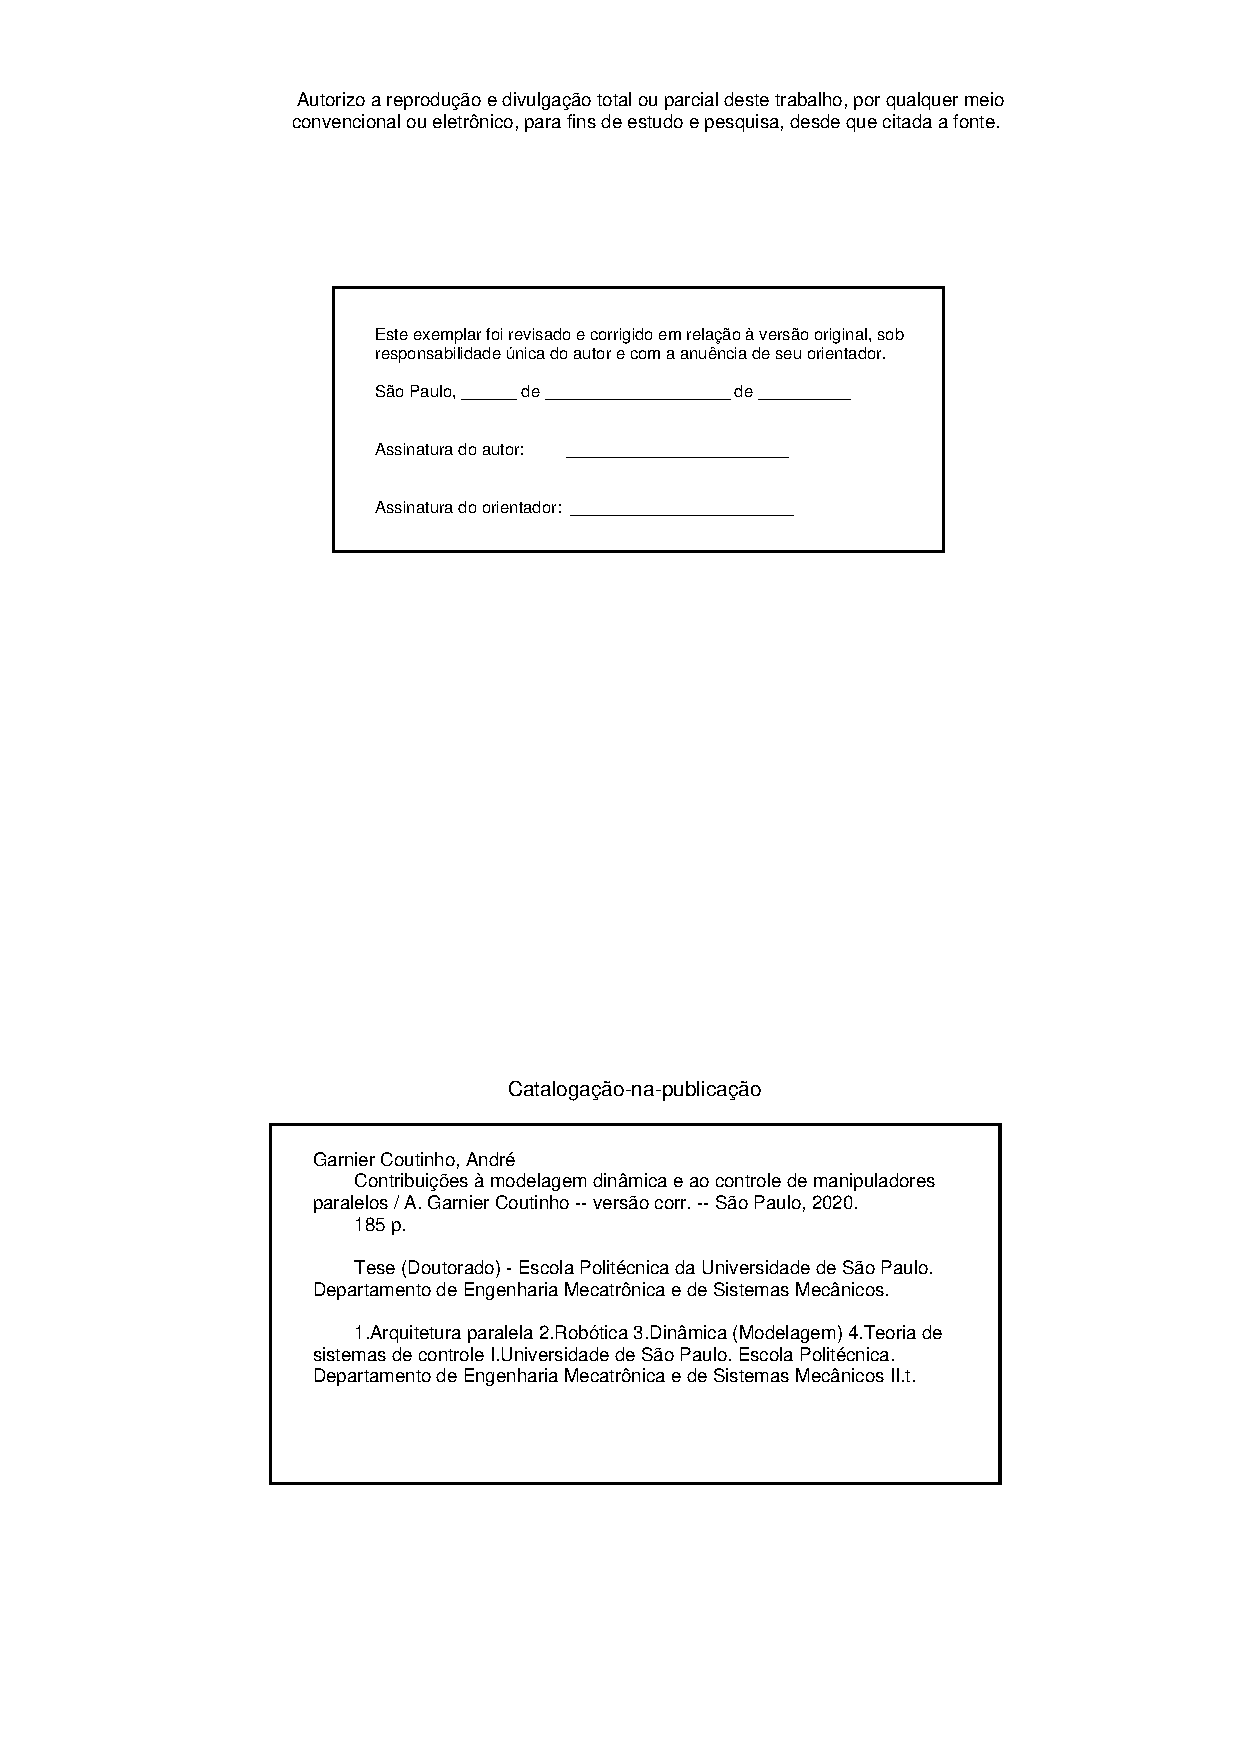
\includepdf[pages=1]{FichaCatalografica.pdf}
\clearpage\thispagestyle{empty}\addtocounter{page}{-1} \clearpage


% ========== Folha de assinaturas (opcional) ==========
%\begin{folhadeaprovacao}
%	\assinatura{Prof. Dr. Tarcisio Antonio Hess Coelho}
%	\assinatura{Prof. Dr. Renato Maia Matarazzo Orsino}
%	\assinatura{Profª. Dra. Maira Martins da Silva}
%	\assinatura{Prof. Dr. Bruno Augusto Angélico}
%	\assinatura{Prof. Dr. Diego Colón}
%\end{folhadeaprovacao}


% ========== Ficha catalográfica ==========
% Fazer solicitação no site:
%	http://www.poli.usp.br/en/bibliotecas/servicos/catalogacao-na-publicacao.html


% ========== Dedicatória (opcional) ==========
%\dedicatoria{Dedicatória}


% ========== Agradecimentos ==========
\begin{agradecimentos}

Gostaria de agradecer a todos que sempre me apoiaram e ajudaram a perseguir o meu sonho de me tornar Doutor em Engenharia Mecânica pela Escola Politécnia da USP. Não tenho palavras para descrever o que significa para mim poder estar contribuindo ativamente na exploração das fronteiras do conhecimento.

Dentre as várias pessoas que sempre estiveram ao meu lado nesta jornada, gostaria de destacar o meu orientador e amigo Prof. Dr. Tarcisio Antonio Hess Coelho, o qual sempre esteve ao meu lado desde o início da jornada no meio acadêmico, sempre sendo super solícito, me apoiando, e me orientando da melhor maneira possível; meu grande amigo Prof. Dr. Renato Maia Matarazzo Orsino, o qual me introduziu e ensinou o que há de mais sofisticado e eficiente na parte de modelagem de sistemas multicorpos, um conhecimento fundamental para o desenvolvimento desta tese, também sempre sendo extremamente solícito e me ajudando sempre que podia; aos grandes amigos Engª. Juliana Martins de Oliveira Fuess e Eng. Victor Pacheco Bartholomeu, os quais participaram ativamente e possibilitaram o desenvolvimento do protótipo de manipulador paralelo que possibilitou adicionar um caráter experimental na tese desenvolvida; à minha namorada Adriana Marques Cavalcanti, a qual está há mais de 12 anos ao meu lado, sempre me apoiando em todos os momentos e me inspirando a ser cada vez mais uma pessoa melhor; e aos meus pais Antonio Valdec Martins Coutinho e Taïs Borges Garnier, e avó Maria Luiza Borges Garnier, os quais sempre se preocuparam muito comigo, sempre me apoiando e ajudando de todas as maneiras.

Por último, mas não menos importante, além dessas pessoas incríveis que tive a oportunidade de conhecer em minha vida, gostaria de destacar meu agradecimento a outras três pessoas maravilhosas que conheci há pouco tempo, que mudaram minha vida, e que tornaram possível a conclusão desta tese de doutorado: minha psicóloga Dra. Ana Maria Canzonieri, minha psiquiatra Dra. Letícia Pacheco Lessa, e minha professora de yoga Alessandra Dotto.

Muito obrigado a todos, sem vocês nada disso seria possível.

\end{agradecimentos}


% ========== Epígrafe (opcional) ==========
\epigrafe{%
	\emph{`` `Nesta direção', disse o Gato, girando a pata direita, `mora um Chapeleiro. E nesta direção', apontando com a pata esquerda, `mora uma Lebre de Março. Visite quem você quiser, são ambos loucos.' \\
	`Mas eu não ando com loucos', observou Alice. \\
	`Oh, você não tem como evitar', disse o Gato, `somos todos loucos por aqui. Eu sou louco. Você é louca'. \\
	`Como é que você sabe que eu sou louca?', disse Alice. \\
	`Você deve ser', disse o Gato, `Senão não teria vindo para cá.' ''}
	\begin{flushright}
		-{}- Lewis Carroll
	\end{flushright}
}


% ========== Resumo ==========
\begin{resumo}
Os mecanismos paralelos são conhecidos por suas características promissoras, como alta rigidez estrutural,  alta precisão de posicionamento, baixa inércia, e alta capacidade de carga. Estas características os tornam muito atraentes para realizar tarefas em que são necessárias grandes velocidades e acelerações, como {\em pick-and-place}, ou grande rigidez e precisão, como usinagem e posicionamente de telescópios.

No entanto, dada a sua maior complexidade mecânica, os modelos dinâmicos se tornam muito mais complexos e de dificil obtenção, o que pode dificultar muito a tarefa do controle, e consequentemente levar a uma não exploração de todo o potencial que estes mecanismos tem a oferecer.

Dado o alto grau de acoplamento e de não linearidades deste tipo de sistema, a utilização de técnicas de controle não baseadas em modelo pode deixar muito a desejar. Por outro lado, dada a grande complexidade dos modelos, a utilização de técnicas de controles baseadas em modelo pode ser de difícil implementação e de alto custo computacional.

Com o intuito de explorar ao máximo o potêncial deste tipo de arquitetura, nesta Tese são feitos o desenvolvimento de algoritmos de modelagem cinemática e dinâmica, os quais facilitam muito o processo de modelagem e de implementação em tempo real, projetos de controladores robustos baseados em modelo, de modo a diminuir a sensibilidade a incertezas do modelo, e a validação experimental dos controladores propostos em um mecanismo do tipo pentágono articulado, comparando-os com outras técnicas de controle frequentemente utilizadas na literatura.
%
\\[3\baselineskip]
%

%Detelhar mais o mecanismo, a bancada, a finalidade do controle, dizer quais técnicas, "os resultados experimentais obtidos mostram..."

\textbf{Palavras-Chave} -- Mecanismos paralelos, Robótica, Modelagem dinâmica , Controle, Controle não linear.
\end{resumo}


% ========== Abstract ==========
\begin{abstract}
Parallel mechanisms are known for their promising features, such as high structural stiffness, high precision in positioning, low inertia, and high load carrying capacity. These features make them very attractive to perform tasks in which high speeds and accelerations, such as pick-and-place, or high stiffness and precision, such as milling and telescope positioning, are needed.

However, given their greater mechanical complexity, the dynamic models become much more complex and hard to obtain, making the control task more difficult, and consequently leading to a non-exploration of all the potential these mechanisms have to offer.

Given the high degree of dynamic coupling and non-linearities of this kind of system, the use of control techniques that are not model-based may not be the best solution. On the other hand, due to the great complexity of the dynamic models, the use of model-based control techniques may be difficult to implement and may have a high computational cost.

Aiming to fully explore the potential of this kind of architecture, in this thesis are developed kinematic and dynamic modelling algorithms, which greatly facilitate the modelling and real-time implementation process, robust model-based controller designs, in order to reduce the uncertainty sensitivity of the model, and validation of the proposed controllers in an articulated pentagon type mechanism, comparing them with other control techniques frequently used in the literature.
%
\\[3\baselineskip]
%
\textbf{Keywords} -- Parallel mechanisms, Robotics, Dynamic modelling, Control, Non-linear control
\end{abstract}


% ========== Listas (opcional) ==========
\listadefiguras
\listadetabelas
\chapter*{Lista de Símbolos e Convenções}

\begin{center} \begin{Large} \textbf{Alfabetos matemáticos} \end{Large} \end{center}
\begin{longtable}{lp{0.6\textwidth}}
  $a, b, \hdots $ & Escalares, componentes de matrizes-coluna, componentes de matrizes ou índices \\
  $\underline{a}, \underline{b}, \hdots $ & Matrizes diagonais \\
  $A, B, \hdots$ & Escalares, componentes de matrizes-coluna ou componentes de matrizes \\
  $\ma, \mb, \hdots$ & Matrizes-coluna \\
  $\breve{\ma}, \breve{\mb}, \hdots$ & Quaternions \\
  $\mA, \mB, \hdots$ & Matrizes \\
  $\va, \vb, \hdots$ & Vetores físicos \\
  $\hat{\va}, \hat{\vb}, \hdots$ & Versores físicos \\
  $\vA, \vB, \hdots$ & Tensores físicos de segunda ordem ou transformações lineares \\
  $\tta, \ttb, \hdots$ & Pontos no espaço \\
  $\ttA, \ttB, \hdots$ & Sistemas de coordenadas \\
  $\llA, \llB, \hdots$ & Corpos rígidos ou referenciais \\
  $\ssA, \ssB, \hdots$ & Sistema ou subsistema mecânico \\
\end{longtable}
\begin{center} \begin{Large} \textbf{Convenções de matrizes} \end{Large} \end{center}
\begin{longtable}{lp{0.6\textwidth}}
  $\ma \llbracket i \rrbracket $ & i-ésimo elemento da matriz-coluna $\ma$ \\
  $\mA \llbracket i,j \rrbracket $ & elemento da i-ésima linha e j-ésima coluna da matriz $\mA$ \\
  $\mA \llbracket i,: \rrbracket $ & i-ésima linha da matriz $\mA$ \\
  $\mA \llbracket :,j \rrbracket $ & j-ésima coluna da matriz $\mA$ \\
\end{longtable}
\newpage
\begin{center} \begin{Large} \textbf{Representações matriciais de pontos e vetores} \end{Large} \end{center}
\begin{longtable}{lp{0.6\textwidth}}
  $\vct{\ttp}_{\ttB}$ & Matriz-coluna formada pelas coordenadas do ponto $\ttp$ no sistema de coordenadas $\ttB$ \\
  $\hvct{\ttp}_{\ttB}$ & Matriz-coluna formada pelas coordenadas do ponto $\ttp$ no sistema de coordenadas $\ttB$ em coordenadas homog\^eneas, ou seja: $\hvct{\ttp}_{\ttB} = \begin{bmatrix}
[\ttp]_{\ttB} \\
1
\end{bmatrix} $ \\
  $[\vu]_{\ttB}$ & Matriz-coluna formada pelas componentes do vetor $\vu$ na base do sistema de coordenadas $\ttB$ \\
\end{longtable}
\begin{center} \begin{Large} \textbf{Representação de Matrizes de Rotação e Transformação Homogênea} \end{Large} \end{center}
\begin{longtable}{lp{0.6\textwidth}}
  $\nvct{\vone}_{\ttA \rl \ttB} $ & Matriz de mudança de base, i.e. $\nvct{\vu}_{\ttA} = \nvct{\vone}_{\ttA \rl \ttB} \cdot \nvct{\vu}_{\ttB} $ \\
  $\hvct{\vone}_{\ttA \rl \ttB}$ & Matriz de transformação homogênea, i.e. $\hvct{\ttp}_{\ttA} = \hvct{\vone}_{\ttA \rl \ttB} \cdot \hvct{\ttp}_{\ttB}$ \\
\end{longtable}
\begin{center} \begin{Large} \textbf{Vetores e Tensores} \end{Large} \end{center}
\begin{longtable}{lp{0.6\textwidth}}
  $\vgamma$ & Vetor aceleração gravitacional \\
  $\vr_{\tta \rl \ttb}$ & Vetor que liga o ponto $\tta$ ao ponto $\ttb$, orientado no sentido de $\tta$ até $\ttb$ \\
  $\vv_\ttp^{\lllA}$ & Vetor velocidade do ponto $\ttp$ em relação ao ref. $\llA$ \\
  $\va_\ttp^{\lllA}$ & Vetor velocidade do ponto $\ttp$ em relação ao ref. $\llA$ \\
  $\vomega_{\lllB}^{\lllA}$ & Vetor velocidade angular do corpo rígido (ou referencial) $\llB$ em relação ao referencial $\llA$ \\
  $\valpha_{\lllB}^{\lllA}$ & Vetor aceleração angular do corpo rígido (ou referencial) $\llB$ em relação ao referencial $\llA$ \\
  $\vf_{\lllB}$ & Vetor força não reativa aplicada no centro de massa do corpo rígido $\llB$ \\
  $\vtau_{\lllB}$ & Vetor torque não reativo aplicada no corpo rígido $\llB$ \\
  $\vI_{\lllB}$ & Tensor de inércia do corpo rígido $\llB$ em relação a seu centro de massa \\
  $\vzr$ & Vetor nulo \\
  $\vone$ & Tensor identidade \\
  $\{\vi_\ttB, \vj_\ttB, \vk_\ttB \}$ & Base ortonormal do sistema de coordenadas $\ttB$ \\
\end{longtable}
\begin{center} \begin{Large} \textbf{Pontos} \end{Large} \end{center}
\begin{longtable}{lp{0.6\textwidth}}
  $\ttc_{\lllB}$ & Centro de massa do corpo rígido $\llB$ \\
  $\tto_{\ttB}$ & Origem dos sistema de coordenadas $\ttB$ \\
\end{longtable}
\begin{center} \begin{Large} \textbf{Referenciais} \end{Large} \end{center}
\begin{longtable}{lp{0.6\textwidth}}
  $\llN$ & Referencial inercial \\
\end{longtable}
\begin{center} \begin{Large} \textbf{Matrizes} \end{Large} \end{center}
\begin{longtable}{lp{0.6\textwidth}}
  $\mq$ & Coordenadas generalizadas \\
  $\mpi$ & Quasi-coordenadas \\
  $\mp$ & Quasi-velocidades \\
  $\dot{\mp}$ & Quasi-acelerações \\
  $\mu$ & Esforços ativos generalizados (provenientes de atuadores) \\
  $\mM$ & Matriz de inércia generalizada \\
  $\mnu$ & Matriz-coluna de esforços inérciais giroscópicos e de atrito generalizados \\
  $\mg$ & Matriz-coluna de esforços gravitacionais generalizados \\
  $\mzr$ & Matriz-coluna nula ou matriz nula \\
  $\mone$ & Matriz identidade \\
\end{longtable}
\begin{center} \begin{Large} \textbf{Escalares} \end{Large} \end{center}
\begin{longtable}{lp{0.6\textwidth}}
  $\dl W$ & Trabalho virtual \\
  $m$ & Massa \\
  $J$ & Momento de inércia \\
  $b$ & Coeficiente de atrito viscoso \\
  $\gmu$ & Coeficiente de atrito seco \\
  $i$ & Corrente elétrica ou índice genérico \\
  $u$ & Tensão elétrica \\
  $\omega$ & Velocidade angular \\
  $k_e$ & Constante de força contra-eletromotriz \\
  $R$ & Resistência elétrica \\
  $L$ & Indutância \\
  $t$ & Tempo \\
\end{longtable}
\begin{center} \begin{Large} \textbf{Funções} \end{Large} \end{center}
\begin{longtable}{lp{0.6\textwidth}}
  $\ccos(.)$ & Notação compacta para $\cos(.)$ \\
  $\ssin(.)$ & Notação compacta para $\sin(.)$ \\
  $\sign(.)$ & Função sinal \\
  $\diag(.)$ & Matriz-coluna cujos elementos são a diagonal de uma matriz quadrada \\
  $\mS(.)$ & Matriz de produto vetorial entre matrizes-colunas de ordem 3, ou seja, $\vct{\va \wedge \vb}_{\ttA} = \mS(\ma) \cdot \mb = -\mS(\mb) \cdot \ma $, sendo $\ma = \vct{\va}_{\ttA}$ e $\mb = \vct{\vb}_{\ttA}$ \\
\end{longtable}
\begin{center} \begin{Large} \textbf{Operadores} \end{Large} \end{center}
\begin{longtable}{lp{0.6\textwidth}}
  $\dd$ & Operador diferencial \\
  $\dl$ & Operador variação \\
  $\displaystyle\frac{\del (.)}{\del x} = \partial_x (.)$ & Derivada parcial em relação ao escalar $x$ \\
  \addlinespace[0.2cm]
  $\displaystyle\frac{\del (.)}{\del \mx} = \partial_\mx (.)$ & Gradiente ou jacobiano em relação à matriz-coluna $\mx$ \\
  \addlinespace[0.2cm]
  $\displaystyle\frac{\dd (\boxdot) }{\dd t} = (\dot{\boxdot})$ & Operador derivada temporal \\
  \addlinespace[0.2cm]
  $\displaystyle\frac{\dd^{[\lllA]}(\boxdot)}{\dd t} = (\dot{\boxdot}^{[\lllA]})$ & Operador derivada temporal em relação ao referencial $\llA$ (se aplica apenas a vetores físicos) \\
  $\wedge$ & Operador produto vetorial \\
  $\otimes$ & Operador produto de quaternions \\
  $\ntmat{\cdot}$ & Matriz transposta \\
  $\nimat{\cdot}$ & Matriz inversa \\
  $\npmat{\cdot}$ & Matriz pseudo-inversa \\
  $\nmmat{\cdot}$ & Módulo aplicado em cada componente de uma matriz ou matriz-coluna
\end{longtable}

% ========== Sumário ==========
\sumario



% ========== Elementos textuais ==========

\part{Introdução}
	
\chapter{Introdução}
\capepigrafe[0.5\textwidth]{``A única forma de chegar ao impossível é acreditar que é possível''}{Lewis Carroll}

Os mecanismos de arquitetura paralela são amplamente utilizados em simuladores de voo, simuladores automobilisticos, e tarefas de {\em pick-and-place}. Além disso, também são empregados em sistemas de posicionamento, sistemas de medição, máquinas de usinagem, entre outras tarefas. 

Este tipo de arquitetura há mais de duas décadas já atrai pesquisadores e instituições com o intuito de investigar seu grande potencial em vários quesitos, como capacidade de carga, precisão de posicionamento, rigidez estrutural, consumo energético, baixa inércia, e de atingir altas velocidades e acelerações \cite{Cheng, Khalil, Merlet2002, Pashkevich, Tsai}. Grande parte deste potencial se deve à possibilidade de instalação de todos os motores na base imóvel do mecanismo, o que diminui significativamente sua a inércia. 

Atualmente, este grande potencial já consegue ser muito bem explorado em tarefas de {\em pick-and-place} \cite{Clavel} e usinagem \cite{Pashkevich}, entre outras. Porém, essas características promissoras muitas vezes vem ao custo de algumas inconveniências associadas a este tipo de arquitetura, como o grande número de componentes mecânicos, um espaço de trabalho mais limitado, e um modelo dinâmico muito mais complexo e de difícil obtenção \cite{Rynaldo, Merlet2002}. Boa parte destas desvantagens, porém, podem ser contornadas através da escolha cuidadosa das juntas utilizadas, dos parâmetros cinemáticos, da topologia e do design mecânico \cite{Briot, Campos, Jiang, Zhan}, como é feito no robô Adept Quattro (figura\ref{fig:Mecanismo}).

\begin{figure}[h]
	\centering
	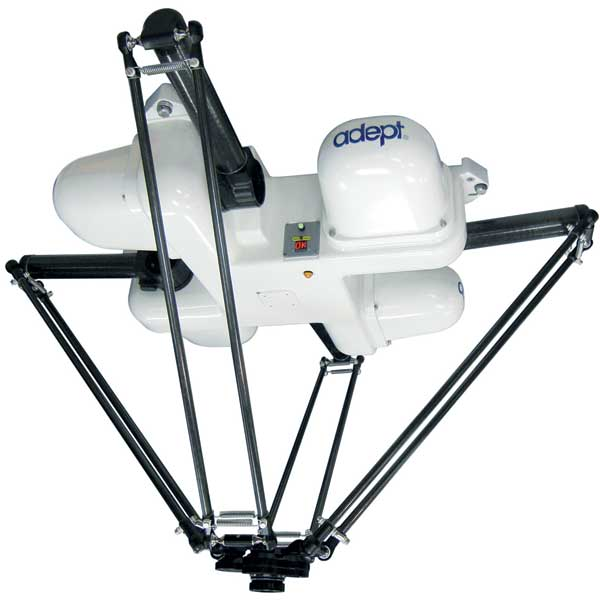
\includegraphics[scale=0.17]{../figures/theadeptquat.jpg}  
	\caption{Robô industrial Adept Quattro - Retirada de PhysOrg.com}
	\label{fig:Mecanismo}
\end{figure}

Levando-se em conta esta dificuldade de obtenção e a complexidade inerente do modelo dinâmico, o controle de mecanismos de arquitetura paralela é uma tarefa desafiadora. A utilização de estratégias de controle não baseadas em modelo pode deixar muito a desejar na exploração do potencial que estes mecanismos oferecem, principalmente em tarefas de seguimento de trajetória \cite{Chung}, e a utilização de modelos dinâmicos simplificados pode limitar significativamente o desempenho do projeto de controladores baseados em modelo, principalmente quando se trabalha com altas velocidades e acelerações. Além disso, mesmo na hipótese do modelo dinâmico completo estar disponível, o emprego de técnicas de controle não linear pode acarretar um custo  computacional muito elevado \cite{Craig, Slotini, Zubizarreta, Zubizarreta3}. Este paradigma, aliado à escassez de trabalhos publicados com comprovação experimental de técnicas de controle aplicáveis a mecanismos paralelos \cite{Rynaldo}, resulta na exploração insatisfatória dos potenciais promissores de tais máquinas, como resposta dinâmica rápida e alta precisão \cite{Abdellatif}.
	
Com o intuito de atacar os problemas da dificuldade de obter modelos dinâmicos completos e diminuir o custo computacional de suas implementações em leis de controle baseadas em modelos, esta tese propõe um algoritmo genérico de modelagem dinâmica de mecanismos paralelos translacionais, o qual pode ser utilizado para calcular previamente termos do modelo dinâmico em um número finito de pontos do espaço de trabalho, sendo necessário apenas o cálculo de interpolações em tempo real.  Além disso, em virtude de existirem poucos  trabalhos publicados apresentando comprovação experimental de técnicas de controle aplicáveis a mecanismos paralelos, nesta tese, são obtidos e apresentados resultados experimentais da implementação de 8 diferentes estratégias de controle, tanto baseadas como não baseadas em modelo, incluindo estratégias de controle não linear robusto. Desta maneira, o trabalho desenvolvido nesta tese visa contribuir para uma melhor exploração do grandes potenciais dos mecanismos com este tipo de arquitetura.


%Além disso, atacando o problema da  escassez de trabalhos publicados com comprovação experimental de técnicas de controle aplicáveis a mecanismos paralelos, são obtidos e apresentados resultados experimentais da implementação de 8 diferentes estratégias de controle, tanto baseadas como não baseadas em modelo, incluindo estratégias de controle não linear robusto. Desta maneira, o trabalho desenvolvido nesta tese visa contribuir para uma melhor exploração do grandes potenciais dos mecanismos com este tipo de arquitetura.
    
    %Uma alternativa para a superação desta dificuldade seria a combinação de técnicas de controle não linear robusto (por exemplo, controle por modos deslizantes \cite{Slotini, Utkin}) com modelos dinâmicos completos de mecanismos paralelos, desenvolvidos a partir de novas metodologias de modelagem de sistemas multicorpos \cite{22orsino, Orsino2013, 23orsino, 21orsino}. Com esta estratégia, torna-se possível sintetizar leis de controle de alto desempenho e custo computacional mais adequado, viabilizando uma maior exploração do potencial promissor dos mecanismos paralelos.

%OBJETIVOS E JUSTIFICATIVAS--------------------------------------------
\section{Objetivos}\label{objetivos}

O objetivo geral desta Tese é contribuir para o aumento do desempenho de manipuladores paralelos. Quanto aos objetivos específicos, propõe-se que este aprimoramento seja realizado mediante o emprego de técnicas de controle baseadas em modelo do manipulador. Neste sentido, almeja-se fornecer recomendações quanto à modelagem dinâmica, à técnica de controle mais adequada, bem como a sua implementação.

%%%%% BASEAR NAS CONTRIBUIÇÕES %%%%%%%%%%%%%%%%

%Os principais objetivos da tese s\~ao:
%\begin{itemize}
%\item Desenvolvimento de um algoritmo gerador de modelos dinâmicos completos de mecanismos paralelos, de forma implícita. Será utilizada uma metodologia baseada no método Orsino de acoplamento de subsistemas multicorpos \cite{23orsino}.


%\item Elabora\c{c}\~ao de metodologias de projeto de controlador n\~ao linear robusto, de alto desempenho, aplicável a  mecanismos de arquitetura paralela. Para tanto, serão consideradas as incertezas param\'etricas e a possibilidade de atua\c{c}\~ao redundante \cite{Cheng},  além de estratégias para a síntese de leis de controle com custo computacional consideralvemente menor do que as tradicionais, que empregam o Controle por Torque Computado \cite{Craig, Zubizarreta}.

%\item Realizar a modelagem cinemática e dinâmica dos mecanismos 5R \cite{22orsino} e 2\underline{R}SU+\underline{P}PaP \cite{Rynaldo, Kumazawa}, utilizando o algoritmo de modelagem desenvolvido.

%\item Realizar o projeto de um controlador de trajetória para os mecanismos escolhidos, utilizando a metodologia de projeto de controle proposta.

%\item Realizar simula\c{c}\~oes dinâmicas utilizando as leis de controle sintetizadas.

%\item Realizar a validação experimental dos controladores projetados no protótipo dos mecanismos 5R, o qual se encontra no laboratório de mecanismos da EPUSP.
%\end{itemize}

%É importante ressaltar que os 5 primeiros objetivos citados já foram parcialmente alcançados e que a arquitetura paralela 2\underline{R}SU+\underline{P}PaP foi desenvolvida pelo grupo de pesquisa do Prof. Dr. Tarcio Antonio Hess Coelho, havendo ainda poucos estudos na literatura sobre ela. %Sendo assim, pode-se afirmar que simulações dinâmicas e validações experimentais de leis de controle não linear robusto neste mecanismo tem caráter inédito.

%SOBRE A ORGANIZAÇÃO DO TEXTO--------------------------------------------
\section{Sobre a organização do texto}\label{organizacao}

O capítulo 2 apresenta a revisão da Literatura sobre o assunto, sendo que a metodologia da pesquisa é descrita no capítulo 3. A seguir, os capítulos 4 e 5 abordam a modelagem dinâmica de manipuladores seriais e paralelos, respectivamente. Com relação ao projeto dos controladores, este assunto é elaborado no capítulo 6. No capítulo 7 são apresentados os resultados mais relevantes desta Tese, além da pertinente discussão. Por fim, no capítulo 8, apresentam-se as principais conclusões da Tese e os temas sugeridos para pesquisa futura.

%REVISAO--------------------------------------------------------------------
\chapter{Revisão da literatura}\label{revision}

Considerando o tema de pesquisa desta Tese, esta revisão se concentrará em tópicos relacionados à modelagem dinâmica e ao controle.


\section{Modelagem dinâmica}

Quando se trata de modelagem dinâmica, os mecanismos seriais possuem características topológicas e cinemáticas que podem ser exploradas para facilitar a geração dos modelos cinemáticos e dinâmicos. Suas estruturas mecânicas correspondem a mecanismos de cadeia aberta, apenas com juntas ativas de um grau de liberdade, rotativas ou prismáticas. Além disso, o número de coordenadas generalizadas coincide com o número de atuadores e com a mobilidade do mecanismo \cite{Craig}. 

De fato, o modelo cinemático pode ser obtido, recursivamente ao longo da cadeia cinemática, pelo emprego de métodos vetoriais ou matriciais, partindo-se da base e se dirigindo ao efetuador \cite{Siciliano}. Tradicionalmente, empregam-se os vetores $\mq$ e $\mx$ para descrever as coordenadas associadas aos atuadores e ao efetuador, respectivamente \cite{Cabral, Carvalho}. Enquanto que o problema direto é de resolução relativamente simples, o problema inverso demanda a realização de um processo mais elaborado. Matematicamente, este corresponde à resolução de um sistema não-linear de equações algébricas. Para algumas topologias que utilizam mecanismos esféricos nos punhos, é possível alcançar o desacoplamento das equações de posição e orientação do efetuador \cite{Waldron}.

Com relação à dinâmica, a geração das equações também pode ser realizada de modo recursivo, partindo-se do efetuador e se dirigindo à base, sendo que a solução do problema inverso é obtida mediante a resolução de um sistema linear de equações algébricas. Por outro lado, a solução do problema dinâmico direto é alcançada pela integração de um sistema de equações diferenciais ordinárias (EDOs) \cite{Featherstone}.

%Não tratar de formalismos clássicos da Mecânica (NE,L,GA etc), apenas citar referências q os descrevam de modo geral (livros, tese Orsino) e de modo específico quando aplicados a manipuladores paralelos (artigos). A seguir, serão tratadas as questões ligadas à topologia dos manipuladores, à geração do modelo, bem como as análises para a sua resolução.



%Neste momento, tratar do manipulador paralelo, sua topologia em comparação com os seriais.

Já quando se trata de mecanismos paralelos, dependendo da complexidade da estrutura, podem existir juntas de 1, 2 ou até 3 graus de liberdade, ativas ou passivas. Além disso, o número de elos geralmente é muito superior. Ao se elaborar o modelo cinemático, é possível notar que haverá um grande número de variáveis, dentre as quais algumas serão consideradas independentes e outras, dependentes \cite{Merlet}.

No início do processo de modelagem, é comum  se realizar um corte nas juntas que conectam o efetuador às cadeias cinemáticas. Deste modo, ocorrerá a decomposição do mecanismo original de cadeia fechada no elo do efetuador e nas demais cadeias. Assim, admite-se que estas cadeias possam ser tratadas como abertas. Consequentemente, as equações cinemáticas, geradas em cada cadeia, expressarão o acoplamento entre as variáveis dependentes e independentes do mecanismo. Além disso, para os manipuladores paralelos, a literatura destaca que o problema inverso da cinemática de posição é menos complexo que o direto \cite{Merlet}. 

Saha e Schielen \cite{Saha} mencionam que a dinâmica inversa, uma vez definida a trajetória do efetuador, determina os esforços dos atuadores necessários para o controle, enquanto que a direta é utilizada em simulações do manipulador com o controlador.

Com relação à dinâmica, Pekal e Fraczek \cite{Pekal2} esclarecem que a solução do problema direto pode ser obtida mediante a resolução de um sistema de equações algébrico-diferenciais (EADs), representado por pelo sistema de equações \eqref{DAE}.

\begin{equation} \label{DAE}
\begin{cases}
\mM \, \ddot{\mq} + \mA^\msT \,\mlambda = \meta \\
\bar{\mq} \, (t,\mq) \, = \, \mzr
\end{cases}
\end{equation}

Sendo
%\begin{equation}
%\meta = \mu - \mnu - \mg
%\end{equation}
\begin{equation}
\mA(t,\mq) = \frac{\partial \bar{\mq}}{\partial \mq}
\end{equation}

Uma alternativa é resolver o sistema representado pela equação \eqref{DAE3}, 

\begin{equation}
\underbrace{\left[ \begin{array}{cc}
\mM & \mA^\msT \\
\mA & \mzr
\end{array}
\right]}_{\mY}
\left[ \begin{array}{c}
\ddot{\mq} \\
\mlambda
\end{array}
\right] =
\left[ \begin{array}{c}
\meta \\
-\mb
\end{array}
\right]
\label{DAE3}
\end{equation}

\vspace{0.5cm}

sendo
\begin{equation}
\mb = \frac{\partial (\mA \dot{\mq})}{\partial \mq} \, \dot{\mq} + 2 \frac{\partial \mA}{\partial t} \, \dot{\mq} + \frac{\partial^2 \bar{\mq}}{\partial t^2}
\end{equation}

cuja solução é equivalente à solução de \eqref{DAE} desde que as condições iniciais respeitem as equações vinculares $\bar{\mq}(t, \mq) = \mzr$.

Para melhorar a precisão associada às restrições de posição e velocidade, recomenda-se substituir $\mb$ por $\mb'$, expresso na equação \eqref{baumgarte}, que é conhecido como método de Baumgarte para a estabilização das restrições \cite{Baumgarte, Featherstone, Nikravesh}, sendo $\hat{\alpha} = \hat{\beta} = 1/t_c$, com  $0.01 \lesssim t_c \lesssim 0.1 $ \cite{Featherstone}. 
%
\begin{equation}
\mb' = \mb + 2\hat{\alpha} \dot{\bar{\mq}} + \hat{\beta}^2 \bar{\mq}
\label{baumgarte}
\end{equation}

%\vspace{0.5cm}

Um outro modo de aprimorar a precisão é alcançado pela separação das coordenadas $\mq$ em dois grupos: independentes $\mq\ssh$ e dependentes $\mq\cir$. Assim, multiplica-se a primeira equação de \eqref{DAE} pelo complemento ortogonal \cite{Kordjazi} de $\mA^\msT$. Pekal e Fraczek \cite{Pekal} discutem várias alternativas de obtenção do complemento ortogonal, dentre elas, destacam-se a decomposição QR, a decomposição em matrizes de autovalores e autovetores e a decomposição em valores singulares (DVS). Com esta ação, eliminam-se os multiplicadores de Lagrange e o número de equações se reduz à mobilidade do mecanismo. Em seguida, utiliza-se de relações cinemáticas para  escrever as acelerações $\ddot{\mq}$ em função de $\ddot{\mq}\ssh$. Por consequência, somente as acelerações e velocidades independentes serão integradas no sistema de equações diferenciais. Além disso, em cada passo de integração, as variáveis dependentes $\mq\cir$ e $\dot{\mq}\cir$ serão calculadas a partir das independentes, estabilizando as restrições de posição e velocidade.

%Quando a matriz dos coeficientes $\mY$ , expressa na Eq.(\ref{DAE1}), for singular, os métodos numéricos normalmente empregados, como decomposição LU ou QR, não serão capazes de resolver o sistema de equações. Neste caso, costuma-se empregar $\mY^\msP$, ou seja, a matriz inversa de Moore-Penrose. Outras formulações, como as de Udwadia-Kalaba, Udwadia-Phohomsiri e baseadas no método dos mínimos quadrados, também foram propostas para tratar as situações em que $\mY$ é singular.

Segundo Mariti \emph{et al.} \cite{Mariti}, expressar o modelo dinâmico por meio de coordenadas redundantes, independentemente do formalismo escolhido, possui como propósito a realização de simulações de sistemas multicorpos, sendo que um exemplo é o software comercial MSC-Adams. No entanto, se a finalidade for o controle de manipuladores, significando que o modelo é parte integrante de implementações que demandem  cálculos em tempo real, a expressão das equações dinâmicas nas coordenadas independentes é necessária.

Além disso, é largamente difundido que a escolha das variáveis cinemáticas independentes recaia sobre as componentes do vetor $\mq^\star$, associadas aos deslocamentos impostos pelos atuadores, e suas derivadas temporais. No entanto, alguns autores \cite{Li, Khalil2} mencionam as vantagens de se escolher as componentes do vetor $\mx$, afirmando que a expressão do modelo dinâmico nestas variáveis é menos complexa.

Na literatura, são conhecidas várias formulações para realizar a modelagem dinâmica de sistemas multicorpos, como os formalismos de Newton-Euler, Lagrange, Gibbs-Appel, Maggi, Boltzmann-Hamel, os métodos de Kane e Udwadia-Kalaba, e os Princípios dos Trabalhos Virtuais e Potências Virtuais \cite{23orsino}. Porém, na literatura de modelagem de mecanismos paralelos, podemos destacar as seguintes formulações como as mais comumente utilizadas:

\begin{itemize}
\item Formalismo de Newton-Euler
\item Formalismo de Lagrange
\item Princípio dos Trabalhos Virtuais e das Potências Virtuais
\item Formalismo de Boltzmann-Hamel
\item Método de Kane
\item Formulação do Complemento Ortogonal Natural
\end{itemize}

\subsection{Formalismo de Newton-Euler}

A utilização do formalismo de Newton-Euler é bastante popular para a realização de simulações dinâmicas de mecanismos seriais, tendo em vista que foram desenvolvidos algoritmos recursivos super eficientes para a aplicação deste formalismo neste tipo de arquitetura, como pode ser visto em Featherstone \emph{et al.} \cite{Featherstone}. Porém, para se beneficiar deste tipo de estratégia em mecanismos paralelos, é necessária a utilização de algoritmos de fechamento de malha, os quais aumentam consideravelmente o custo computacional das simulações. Provavelmente por esta razão, aliada à questão da complexidade de implementação dos algoritmos, não foram encontrados na literatura artigos aplicando esta estratégia na modelagem de mecanismos paralelos. 

Apesar da desvantagem de ter que trabalhar com forças reativas no equacionamento, não é raro encontrar na literatura trabalhos que o utilizem. Dentre estes, podemos citar os trabalhos de Arian \emph{et al.} \cite{Arian}, Dasgupta \emph{et al.} \cite{Dasgupta}, Li \emph{et al.} \cite{LiWang}, Shiau \emph{et al.} \cite{Shiau} e Zhang \emph{et al.} \cite{Zhang}.

Em \cite{Arian}, \cite{LiWang} e \cite{Dasgupta}, são feitas a simulações dinâmicas inversas de mecanismos paralelos, de 3 graus de liberdade, nos dois primeiros trabalhos, e de 6 graus de liberdade, no último, utilizando o formalismo de Newton-Euler. Em \cite{Arian} e \cite{LiWang} as simulações são comparadas com \emph{softwares} comerciais. Em \cite{Arian}, também é feita a modelagem utilizando o princípio dos trabalhos virtuais, e são comparados o número de operações e o tempo médio gasto por operação em cada formulação. Como era de se esperar, a formulação do Princípio dos Trabalhos Virtuais se mostrou muito mais eficiente em ambos os quesitos, tendo em vista que não são realizados os cálculos dos esforços reativos. Em \cite{Dasgupta} foi feita uma eliminação de boa parte dos esforços vinculares utilizando manipulações algébricas, o que possibilitou reduzir bastante o custo computacional da simulação.

Em \cite{Shiau} e \cite{Zhang}, os mecanismos paralelos 3-PRS e 3-RRR, respectivamente, são modelados  também utilizando o formalismo de Newton-Euler. Em ambos os trabalhos é considerado o efeito de folgas, e em \cite{Shiau} também o de atritos. A partir dos modelos obtidos, em ambos são feitas simulações dinâmicas diretas. Em \cite{Zhang} é utilizado o método de estabilização de Baumgarte \cite{Baumgarte} para estabilizar a integração numérica. Em \cite{Shiau}, além das simulações, é feita a linearização do modelo dinâmico para determinar as frequências naturais do mecanismo em função da posição do efetuador.

\subsection{Formalismo de Lagrange}

Formulações baseadas na mecânica analítica em geral são muito mais atrativas para realizar a modelagem de mecanismos paralelos, tendo em vista que os esforços vinculares não mais aparecem no equacionamento. Isso justifica a popularidade das escolhas pelo formalismo de Lagrange e pelos Princípios dos Trabalhos Virtuais e das Potências Virtuais para realizar esta tarefa.

Dentre os trabalhos que utilizam o formalismo de Lagrange, podemos citar os trabalhos de  Li \emph{et al.} \cite{Li3}, Singh \emph{et al.} \cite{Singh, Singh2, Singh3} e Yao \emph{et al.} \cite{Yao}.

Em \cite{Singh}, \cite{Singh2} e \cite{Singh3}, são modelados 3 mecanismos paralelos planos de 3 graus de liberdade utilizando o formalismo de Lagrange. Em todos, são realizadas simulações dinâmicas diretas comparando o desempenho de diversas leis de controle. Apenas em \cite{Singh2} é realizada uma dedução completa do modelo dinâmico mostrando a expressão deduzida do modelo. Curiosamente, são adotadas as coordenadas do efetuador como coordenadas generalizadas, e a dedução se mostra relativamente simples para essa arquitetura escolhida, com essa escolha de variáveis.

Já em \cite{Li3}, um mecanismo paralelo espacial de 3 graus de liberdade é modelado, utilizando o formalismo de Lagrange com multiplicadores e o Princípio dos Trabalhos Virtuais, sendo que no último são utilizadas hipóteses simplificadoras. São realizadas simulações dinâmicas inversas e são comparados os resultados utilizando o modelo completo com os resultados utilizando o modelo simplificado.

Em \cite{Yao}, é feita a simulação dinâmica inversa de um mecanismo ainda mais complexo, de 5 graus de liberdade com atuação redundante, também utilizando o formalismo de Lagrange e métodos de otimização para determinar os esforços. Este trabalho, porém, também mostra muito pouco da dedução. Assim, dados a complexidade do mecanismo e o fato de que não é comentado em lugar nenhum o uso de coordenadas redundantes, imagina-se que o modelo utilizado seja um modelo simplificado.

Além disso, foram encontrados trabalhos que utilizam o Princípio dos Trabalhos Virtuais aliado ao formalismo de Lagrange, os quais entitulam essa combinação de ``formulação de Lagrange-D’Alembert'', dentre os quais podemos citar o de Cheng \emph{et al.} \cite{ChengLiu} e Yen \emph{et al.} \cite{Yen}.

No trabalho de Cheng \emph{et al.} \cite{ChengLiu} a ``formulação de Lagrange-D’Alembert'' é utilizada para deduzir uma formulação de acoplamento de subsistemas. A formulação é utilizada para obter o modelo dinâmico de um mecanismo paralelo de 2 graus de liberdade com atuação redundante. São utilizados os modelos já conhecidos para as cadeias seriais, e é feito o acoplamento dos subsistemas a partir de jacobianos dos vínculos cinemáticos.

Em \cite{Yen}, também é utilizada uma estratégia de acoplamento de subsistemas, também deduzida deduzida a partir da ``formulação de Lagrange-D’Alembert'', para obter o modelo dinâmico de um mecanismo paralelo de 3 graus de liberdade. No entanto, neste trabalho, a estratégia não é apresentada de uma maneira mais geral, podendo dar a impressão ao leitor de que isso só foi possível devido à topologia particular do mecanismo em questão. São realizadas simulações dinâmicas diretas do controle de posição do mecanismo, utilizando as técnicas de controle PID e Controle por Torque Computado, as quais são comparadas com resultados experimentais utilizando as mesmas estratégias de controle.

\subsection{Princípio dos Trabalhos Virtuais e das Potências Virtuais}

Levando-se em conta a revisão feita, não foi percebida uma grande diferença de popularidade entre a utilização dos formalismos de Newton-Euler e Lagrange nos artigos que tratam da modelagem dinâmica de mecanismos paralelos. Porém, uma abordagem que se mostrou extremamente popular foi a utilização das formulações do Princípio dos Trabalhos Virtuais ou do Princípio das Potências Virtuais. Dentre os trabalhos que utilizam estes princípios, podemos citar os trabalhos de Arian \emph{et al.} \cite{Arian} (já comentado), Codourey \emph{et al.} \cite{Codourey, CodoureyBurdet}, Gallardo-Alvarado \emph{et al.} \cite{GallardoAlvarado}, Geike \emph{et al.} \cite{Geike}, Li \emph{et al.} \cite{LiStaicu, Li}, Staicu \emph{et al.} \cite{Staicu, Staicu2, Staicu3, StaicuCarpCiocardia, StaicuLiu, StaicuZhang, StaicuZhangRugescu}, Wu et. al \cite{Wu}, Zhao \emph{et al.} \cite{Zhao, Zhao2} e  Zhu \emph{et al.} \cite{Zhu}.

No trabalhos de Codourey \emph{et al.} \cite{Codourey, CodoureyBurdet} e no de Li \emph{et al.} \cite{Li}, são modelados mecanismos paralelos de 3 graus de liberdade, do tipo DELTA nos dois primeiros, e do tipo 3-PRS no terceiro, utilizando o Princípio dos Trabalhos Virtuais. São desprezadas as inércias distribuídas dos elos ligados à plataforma, e suas massas são distribuídas entre as duas pontas em que cada elo é ligado, de modo a simplificar o processo de modelagem.

Já em \cite{GallardoAlvarado}, é modelado um robô paralelo de 4 graus de liberdade utilizando a teoria das helicóides e o Princípio dos Trabalhos Virtuais.

Em \cite{Geike}, é proposta uma metodologia de modelagem interessante, na qual já se dividem as coordenadas generalizadas em um conjunto de variáveis dependentes e outro de variáveis independentes, utilizando a relação entre seus deslocamentos virtuais para obter as equações de movimento. A metodologia é utilizada para realizar a simulação dinâmica inversa de dois mecanismos paralelos, um de 3 graus de liberdade e outro de 6. Além disso, é discutida qual é a forma mais eficiente de implementação da metodologia desenvolvida.

Nos trabalhos de Staicu \emph{et al.} \cite{Staicu, Staicu2, Staicu3, StaicuCarpCiocardia, StaicuLiu, StaicuZhang, StaicuZhangRugescu} e no de Li \emph{et al.} \cite{LiStaicu} são modelados mecanismos paralelos de 3 graus de liberdade utilizando uma metodologia de modelagem recursiva matricial baseada no Princípio dos Trabalhos Virtuais ou no Princípio das Potências Virtuais, e são realizadas simulações dinâmicas inversas. Esses trabalhos apresentam longos equacionamentos para não precisar recorrer a simplificações; porém, em todos os trabalhos, perto do final da dedução do modelo dinâmico, cita-se que será usada a \emph{equação fundamental da dinâmica de robôs paralelos}, a qual está publicada em \cite{StaicuFrances}. Este artigo, porém, está escrito em francês e é muito difícil de ser encontrado.

Por fim, nos trabalhos de Zhao \emph{et al.} \cite{Zhao, Zhao2} e de Zhu \emph{et al.} \cite{Zhu}, são modelados, utilizando o Princípio dos Trabalhos Virtuais e o conceito de jacobianos dos elos, mecanismos paralelos de 6 graus de liberdade nos dois primeiros, e de 3 graus de liberdade no terceiro, sendo que em \cite{Zhao2} o mecanismo possui atuação redundante. Em todos são realizadas simulações dinâmicas inversas.

\subsection{Método de Kane}

Uma formulação que é bastante popular na literatura de mecanismos seriais, porém não muito popular na literatura de mecanismos paralelos, é o Método de Kane \cite{Kane}. Dentre os poucos trabalhos que utilizam esta formulação para realizar a modelagem dinâmica de mecanismos paralelos, podemos citar os trabalhos de Ben-Horina \emph{et al.} \cite{BenHorina} e Shukla \emph{et al.} \cite{Shukla}.

Em \cite{BenHorina}, é realizada a modelagem dinâmica, utilizando o método de Kane, de um robô paralelo de 6 graus de liberdade, cuja atuação é feita por 3 atuadores planos, os quais apresentam 2 graus de liberdade cada. A modelagem é feita com o auxílio do \emph{software} AUTOLEV. São realizadas simulações dinâmicas inversas do mecanismo proposto, e de mais dois mecanismos de 6 graus de liberdade, para efeito de comparação.

Em \cite{Shukla}, também é realizada a modelagem dinâmica de um mecanismo paralelo de 6 graus de liberdade, uma plataforma de Gough–Stewart, utilizando o método de Kane. São realizadas simulações dinâmicas diretas do controle do mecanismo, considerando a dinâmica dos atuadores, utilizando malhas de controle do tipo PID em cascata e compensadores de atraso.

\subsection{Formalismo de Boltzmann-Hamel}

O Formalismo de Boltzmann-Hamel \cite{Jarzebowska} também não se mostrou muito popular na literatura de modelagem dinâmica de mecanismos paralelos. Dentre os trabalhos encontrados, podemos citar os trabalhos de Abdellatif \emph{et al.} \cite{Abdellatif2} e o de Altuzarra \emph{et al.} \cite{20altuzarra}.

Tanto em \cite{Abdellatif2} quanto em \cite{20altuzarra}, são utilizadas as equações de Boltzmann-Hamel para a deduzir formulações que permitem a obtenção do modelo dinâmico explícito de mecanismos paralelos através dos modelos das cadeias seriais, do efetuador, e jacobianos dos vínculos cinemáticos. Em \cite{20altuzarra}, é utilizada a formulação proposta para obter o modelo dinâmico do mecanismo 3-PRS. Em \cite{Abdellatif2} são apresentadas simulações dinâmicas inversa e direta, sendo esta última com leis de controle baseadas no modelo, de um mecanismo paralelo de 6 graus de liberdade.


\subsection{Formulação do Complemento Ortogonal Natural}

A formulação do Complemento Ortogonal Natural foi proposta por Angeles \emph{et al.} em \cite{Angeles}. Sua principal idéia é projetar as equações dinâmicas de cada corpo rígido do sistema em um espaço ortogonal às reações vinculares. Este procedimento é realizado através da obtenção de um complemento ortogonal ao jacobiano das equações de vínculo obtido através de relações cinemáticas dos \emph{twists} de cada corpo com um conjunto de quasi-velocidades independentes. Formulações similares são bastante exploradas por Orsino \emph{et al.} em \cite{22orsino}, e generalizadas em \cite{23orsino}. Dentre os trabalhos que utilizam esta formulação, podemos citar os trabalhos de Akbarzadeh \emph{et al.} \cite{Akbarzadeh}, Khan \emph{et al.} \cite{Khan} e Xi \emph{et al.} \cite{Xi}.

Em \cite{Akbarzadeh}, é descrita uma metodologia genérica de modelagem dinâmica multi-corpos utilizando a formulação do Complemento Ortogonal Natural. Basicamente são obtidos os modelos dinâmicos desacoplados de cada corpo rígido, utilizando a formulação de Newton-Euler, e é feito o acomplamento das equações dinâmicas através do uso do Complemento Ortogonal Natural. A metodologia proposta é aplicada em um mecanismo paralelo esférico do tipo SST e são realizadas simulações dinâmicas inversa e direta do mecanismo.

Em \cite{Xi}, é realizada a modelagem dinâmica de um mecanismo paralelos de 6 graus de liberdade, do tipo hexapod, utilizando a formulação do Complemento Ortogonal Natural. São realizadas simulações dinâmicas inversas do mecanismos em altas e baixas velocidades.

Por fim, em \cite{Khan}, é proposta uma metodologia recursiva de modelagem baseada na formulação do Complemento Ortogonal Natural. A metodologia proposta é utilizada para a obtenção do modelo dinâmico de um mecanismo paralelo plano do tipo 3-RRR, realizando primeiro a modelagem dinâmica das cadeias seriais, e acoplando-as utilizando o Complemento Ortogonal Natural. Também é realizada a simulação dinâmica inversa do mecanismo, utilizando o modelo obtido.








%%%%%%%%%%%%%%%%%%%%%%%%%%%%%%%%%%%%%%%%%%%%%%%%%%%%%%%%%%%%%%%%%%%%%

\section{Controle}

Existem diversas técnicas propostas pela literatura para realizar o controle de mecanismos paralelos. Dentre elas, podemos destacar:

\begin{itemize}
\item Controle Proporcional-Integral-Derivativo (PID)
\item Controle por Torque Computado (TC)
\item Controle por Torque Computado com pré-alimentação (TCp)
\item Controle por Torque Computado Estendido (TCe)
\item Controle Preditivo Baseado em Modelo (PM)
\item Controle Adaptativo
\item Controle por Modos Deslizantes (MD)
\end{itemize}

\subsection{Controle Proporcional-Integral-Derivativo (PID)}

A técnica mais simples consiste na utilização de malhas do tipo PID, controlando cada junta ativa de maneira independente, considerando a dinâmica do mecanismo como distúrbios de controle. Essa técnica é caracterizada por sua facilidade de projeto e implementação, tanto em hardware quanto em software, além de exibir um desempenho satisfatório para movimento lento. Porém, essa técnica não se mostra adequada para a realização de trajetórias em altas velocidades e/ou acelerações \cite{Honegger, Zubizarreta}. Uma malha típica de PID pode ser vista na figura \ref{fig:PID}.

\begin{figure}[h]
	\centering
	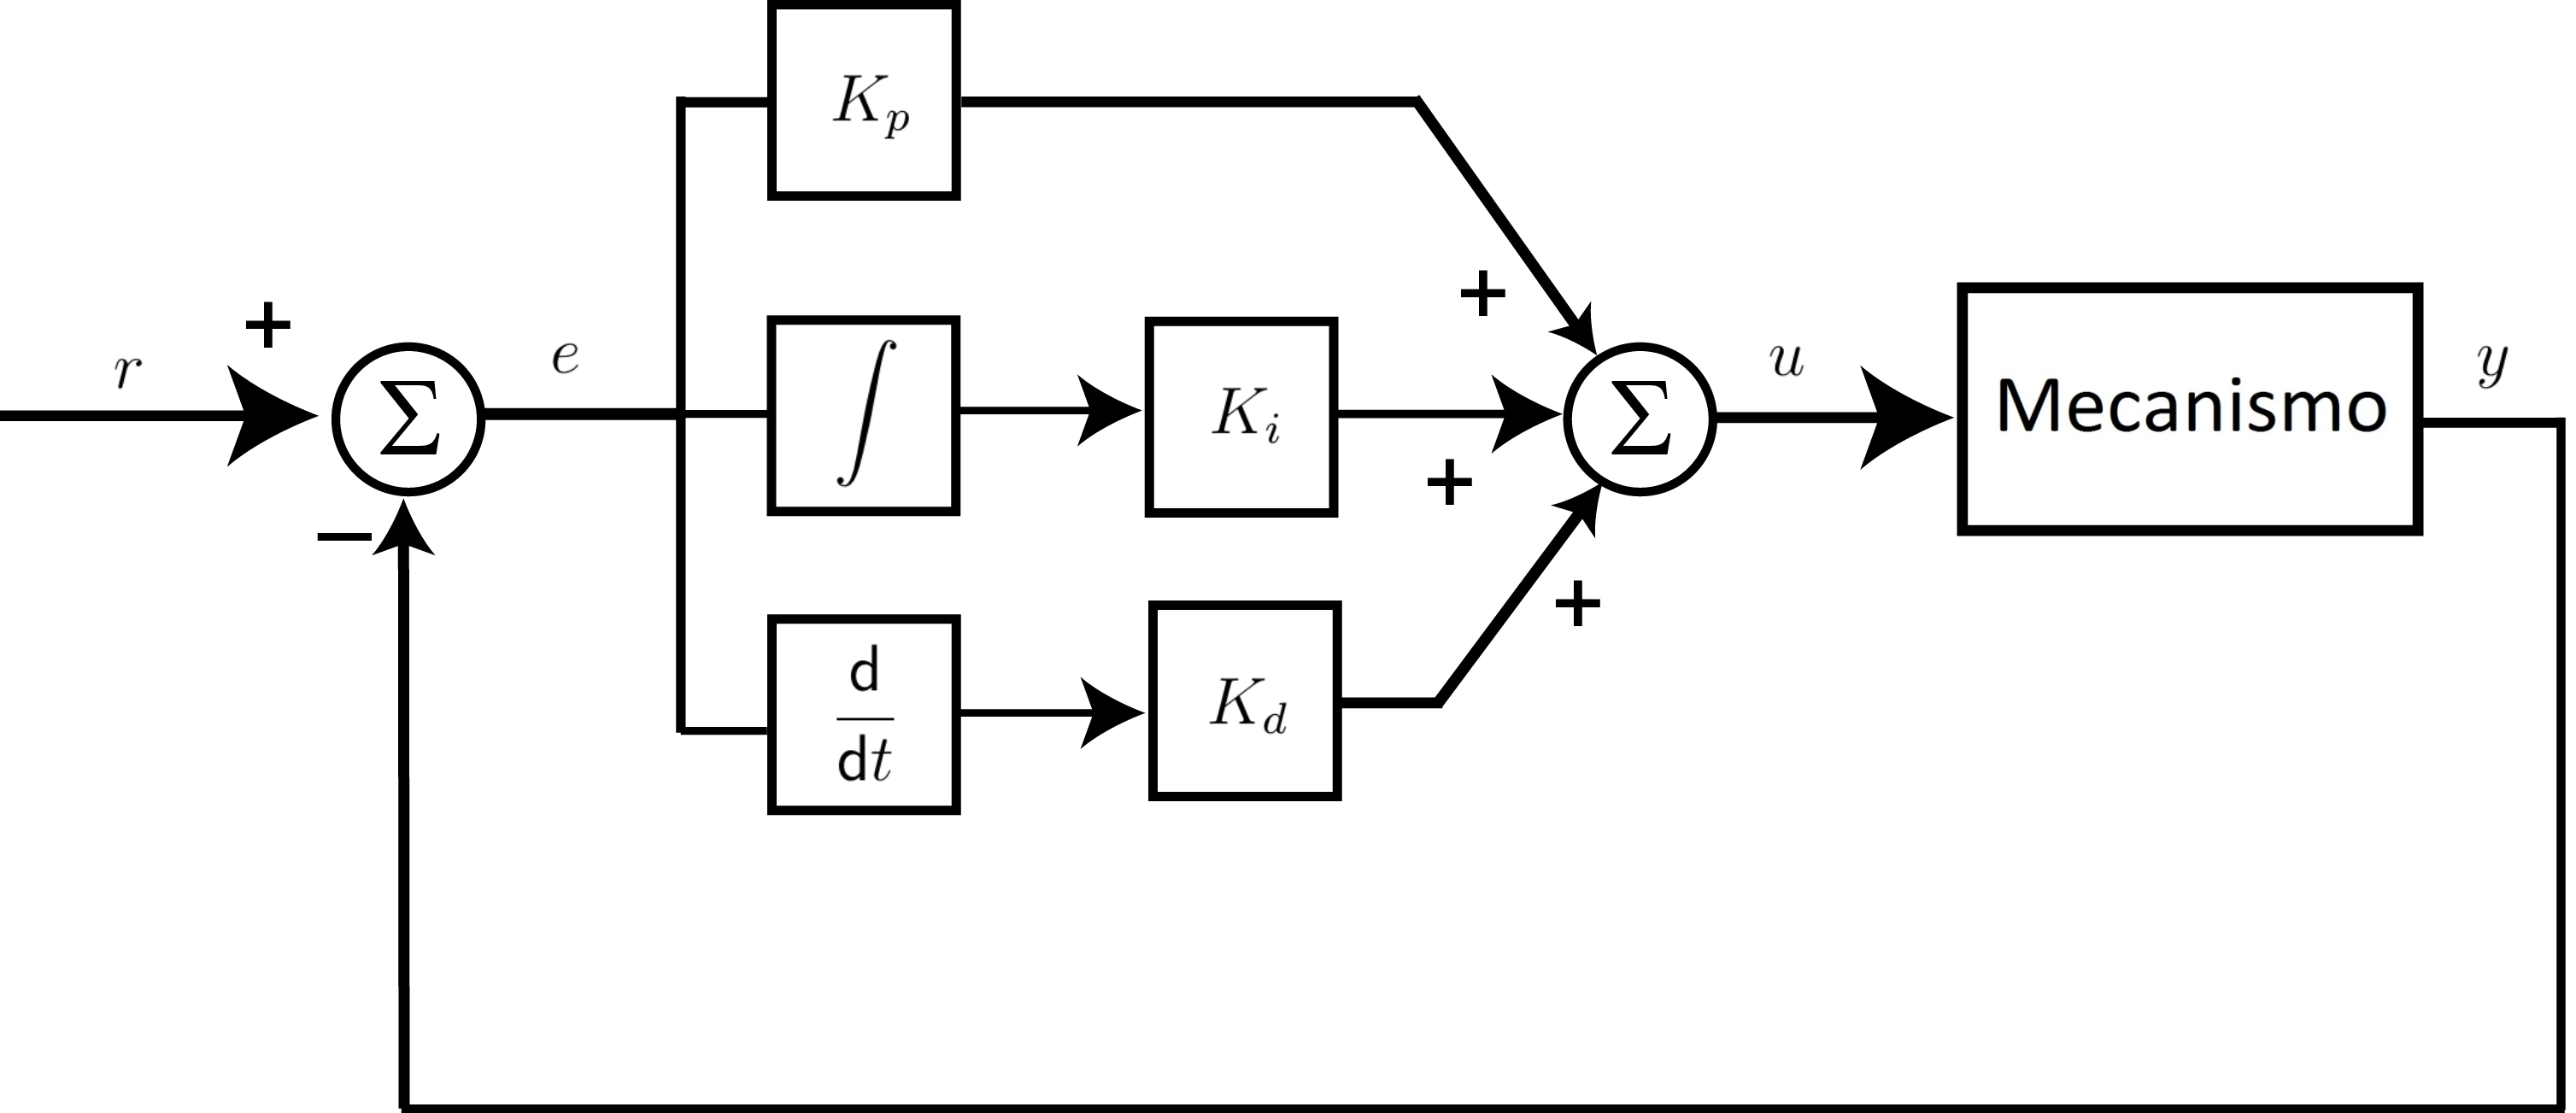
\includegraphics[scale=0.45]{../figures/PID.jpg}  
	\caption{Malha de Controle Proporcional-Integral-Derivativo}
	\label{fig:PID}
\end{figure}

\subsection{Controle por Torque Computado (TC)}

Uma das técnicas de controle mais exploradas na literatura é o Controle por Torque Computado (TC). Basicamente, é um caso particular da técnica de controle não linear conhecida como Linearização pela Realimentação \cite{Slotini}, aplicada a sistemas mecânicos. A técnica consiste na utilização de duas malhas de controle, uma malha que realiza o desacoplamento do sistema e a compensação das não linearidades, e outra malha composta por PIDs independentes \cite{Craig}, como pode ser visto na figura \ref{fig:CTC}. Como resultado, alcança-se um desempenho  superior  àquele obtido utilizando simples PIDs, permitindo inclusive a realização de trajetórias precisas em altas velocidades e/ou acelerações. No entanto, seu desempenho poderá ser limitado pela qualidade/fidelidade do modelo dinâmico utilizado para a compensação das não linearidades \cite{SlotiniSMC}. Sua implementação também é mais complexa, visto que é necessário calcular o modelo dinâmico inverso em tempo real, o que também aumenta consideravelmente seu custo computacional. Além disso, a técnica é sensível a incertezas estruturadas (paramétricas) e não estruturadas (dinâmicas não modeladas). Como exemplos de utilização do TC, podem ser citados os trabalhos de Cheng at al. \cite{Cheng}, Li e Wu \cite{Li}, Li e Fu \cite{Li2}, Shang at al. \cite{Shang} e Yen at al. \cite{Yen}.

\begin{figure}[h]
	\centering
	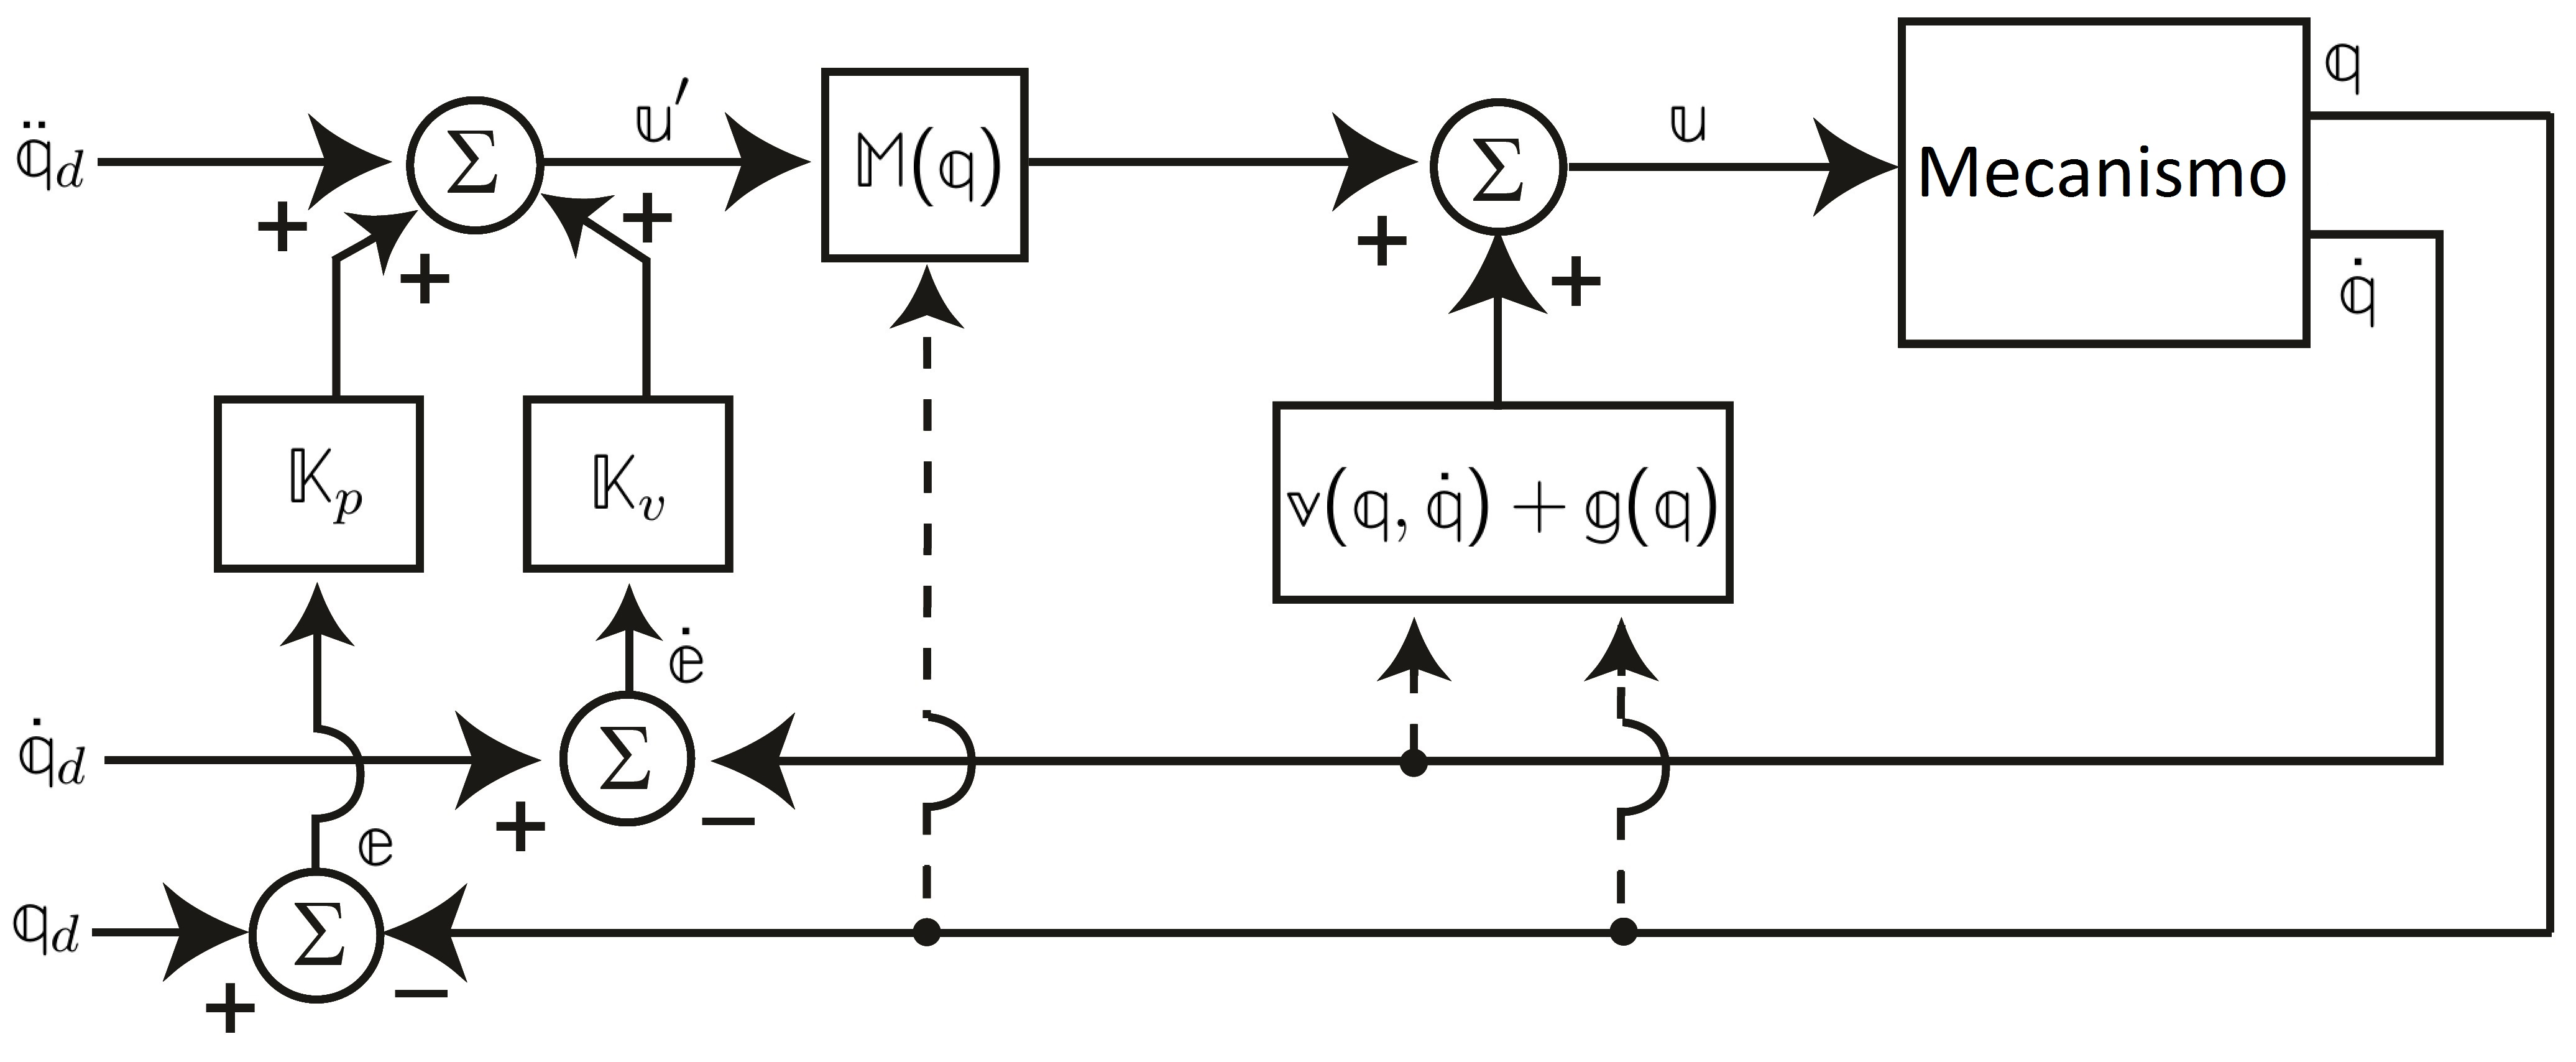
\includegraphics[scale=0.39]{../figures/CTC.jpg}  
	\caption{Malha de Controle por Torque Computado (Adaptado de \cite{Craig})}
	\label{fig:CTC}
\end{figure}

\subsection{Controle por Torque Computado com pré-alimentação (TCp)}

Visando a redução do custo computacional associado ao cálculo do modelo dinâmico em tempo real, alguns autores propõe a utilização do TC com pré-alimentação (TCp) \cite{Khalil, Siciliano, Spong}. Essa técnica é similar ao TC, com a diferença de que a compensação das não linearidades é feita por pré-alimentação e não mais por realimentação, como pode ser visto na figura \ref{fig:CTCp}. Consequentemente, realiza-se o cálculo do modelo dinâmico previamente, diminuindo-se o custo computacional.

De fato, Codourey \cite{Codourey} obteve uma redução de 600\% no erro de posição utilizando o TCp em um ensaio experimental com o robô DELTA, ao substituir os PDs originais. Na simulação do controle de um mecanismo 6-UPS, Wang \emph{et al.} \cite{Wang} utilizaram em cascata controladores lineares de posição, velocidade e corrente em cada junta ativa, além de  uma compensação dinâmica por pré-alimentação dos distúrbios de torque.

\begin{figure}[h]
	\centering
	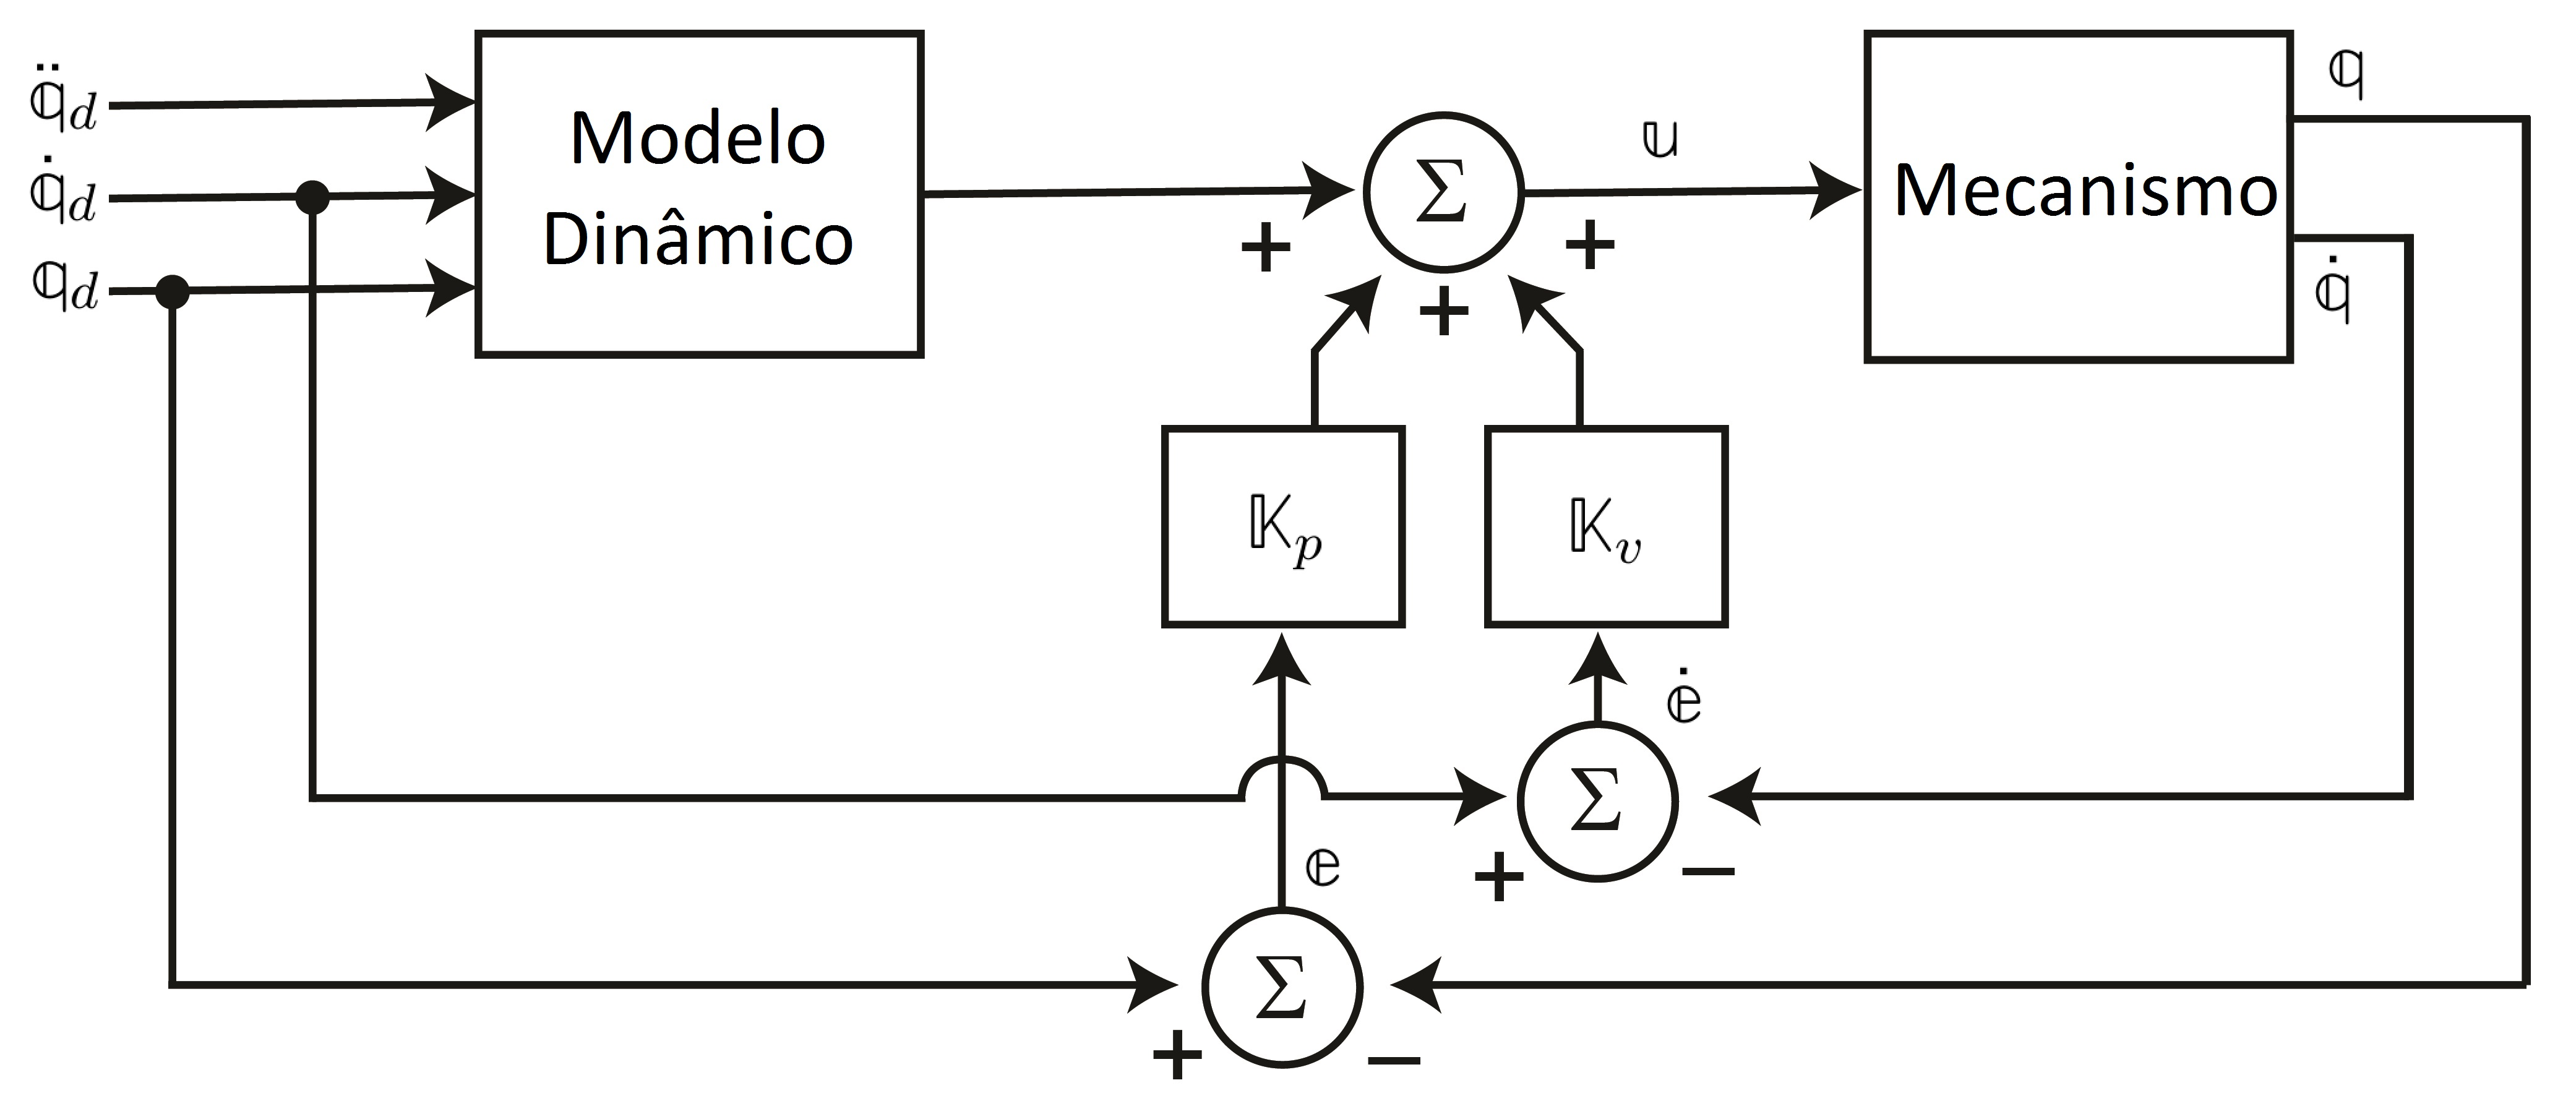
\includegraphics[scale=0.39]{../figures/CTCp.jpg}  
	\caption{Malha de Controle por Torque Computado com pré-alimentação (Adaptado de \cite{Craig})}
	\label{fig:CTCp}
\end{figure}

\subsection{Controle por Torque Computado Estendido (TCe)}

Com o intuito de melhorar a robustez do TC associada a incertezas paramétricas, Zubizarreta \emph{et al.} \cite{Zubizarreta, Zubizarreta2, Zubizarreta3, Zubizarreta4} propuseram  o  Controle por Torque Computado Estendido (TCe), que utiliza informação redundante obtida pelo sensoriamento de juntas passivas. Em \cite{Zubizarreta}, os controladores propostos demonstraram maior robustez, principalmente em relação a parâmetros cinemáticos, durante as simulações realizadas com o mecanismo 3-RRR.

\subsection{Controle Preditivo Baseado em Modelo (PM)}

Outra técnica alternativa, aplicada a mecanismos paralelos, é o Controle Preditivo Baseado em Modelo (PM). Para a sua implementação, o PM necessita minimizar uma função objetivo, dependente das saídas e do esforço de controle, ambos calculados em tempo futuro \cite{Camacho}, como pode ser visto na figura \ref{fig:CPM}. Assim, dependendo do modelo utilizado, o processo de otimização pode agregar um custo computacional que inviabilize o controle, comprometendo a motivação inicial de aprimorar o desempenho do sistema. Como exemplos de utilização do PM, podem ser citados os trabalhos de Vivas \emph{et al.} \cite{Vivas} e   Duchaine \emph{et al.} \cite{Duchaine}.

Com o propósito de controlar o mecanismo H4, Vivas \emph{et al.} \cite{Vivas} utilizaram  uma malha de PM linear e outra malha para compensação das não linearidades. Após a comparação do desempenho do controlador proposto com  o TC, os autores observaram maior robustez do PM a incertezas paramétricas. 

Duchaine \emph{et al.} \cite{Duchaine}, por sua vez, propuseram um controlador preditivo baseado no modelo não linear de um mecanismo paralelo de 6 graus de liberdade. Visando a obtenção de uma solução analítica para o problema de otimização, foram adotadas diversas hipóteses simplificadoras no modelo dinâmico do mecanismo. Com o intuito de comparar o controlador proposto com um PID, foram feitos alguns experimentos, onde se observou  que o PM apresentou erro nulo de posição no final da trajetória, enquanto que o PID demorou um tempo considerável para alcançar erro nulo. Foi verificada a equivalência entre o custo computacional dos 2 controladores. 

\begin{figure}[h]
	\centering
	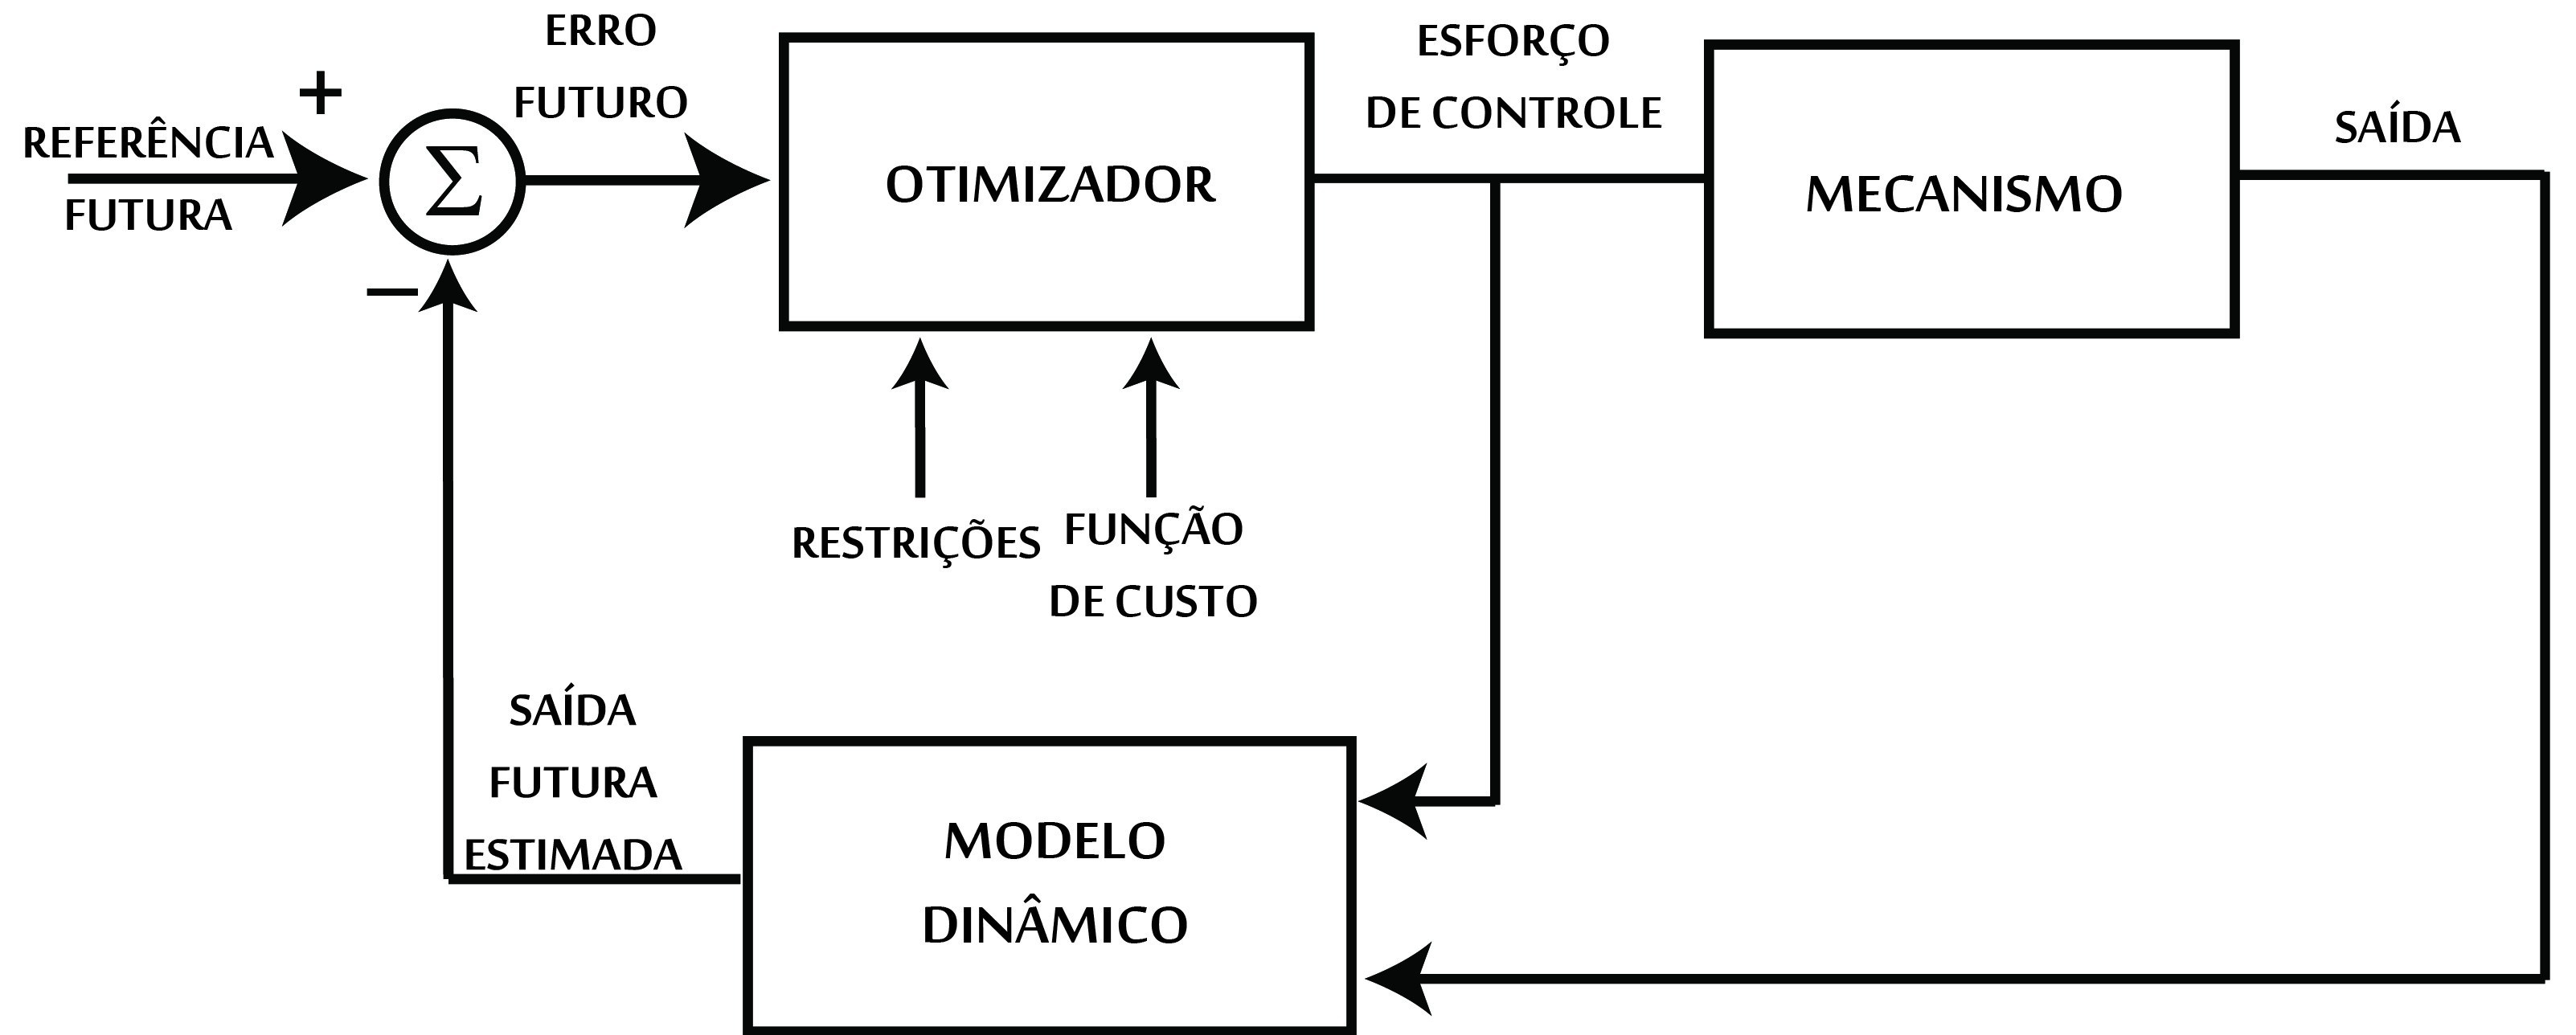
\includegraphics[scale=0.11]{../figures/CPM.jpg}  
	\caption{Malha de Controle Preditivo Baseado em Modelo}
	\label{fig:CPM}
\end{figure}

\subsection{Controle Adaptativo}

O controle adaptativo, também encontrado na literatura, caracteriza-se pela utilização de leis de adaptação para realizar a estimação em tempo real de parâmetros do sistema ou de termos de compensação dinâmica, como pode ser visto na figura \ref{fig:CA}. Sendo assim, as técnicas de controle adaptativo possibilitam que o sistema se torne praticamente insensível a incertezas paramétricas. Para o caso em que se realiza a estimação em tempo real dos parâmetros do sistema, pode-se dizer que o custo computacional é superior ao do TC, visto que é necessário integrar as leis de adaptação em tempo real. Além disso, é necessário obter o modelo dinâmico linear em relação aos parâmetros do sistema \cite{SlotiniA}, o que pode ser uma tarefa difícil, inviabilizando, em alguns casos, a aplicação da técnica. Em \cite{CodoureyBurdet} é proposto um algoritmo de obtenção do modelo dinâmico simplificado de mecanismos paralelos nesse formato.

Em \cite{SlotiniA} é proposta uma lei de controle que combina o controle adaptativo com a técnica de controle robusto conhecida por Controle por Modos Deslizantes. Chemori \emph{et al.} \cite{Chemori} utilizaram essa técnica  com o intuito de diminuir os erros de posição em regime permanente no controle de um mecanismo paralelo do tipo PAR2. Por outro lado, Honegger at al. \cite{Honegger} empregaram o controle adaptativo com estimação em tempo real dos parâmetros do sistemas, realizando a compensação dinâmica por pré-alimentação, em um mecanismo  paralelo do tipo Hexaglide.

\begin{figure}[h]
	\centering
	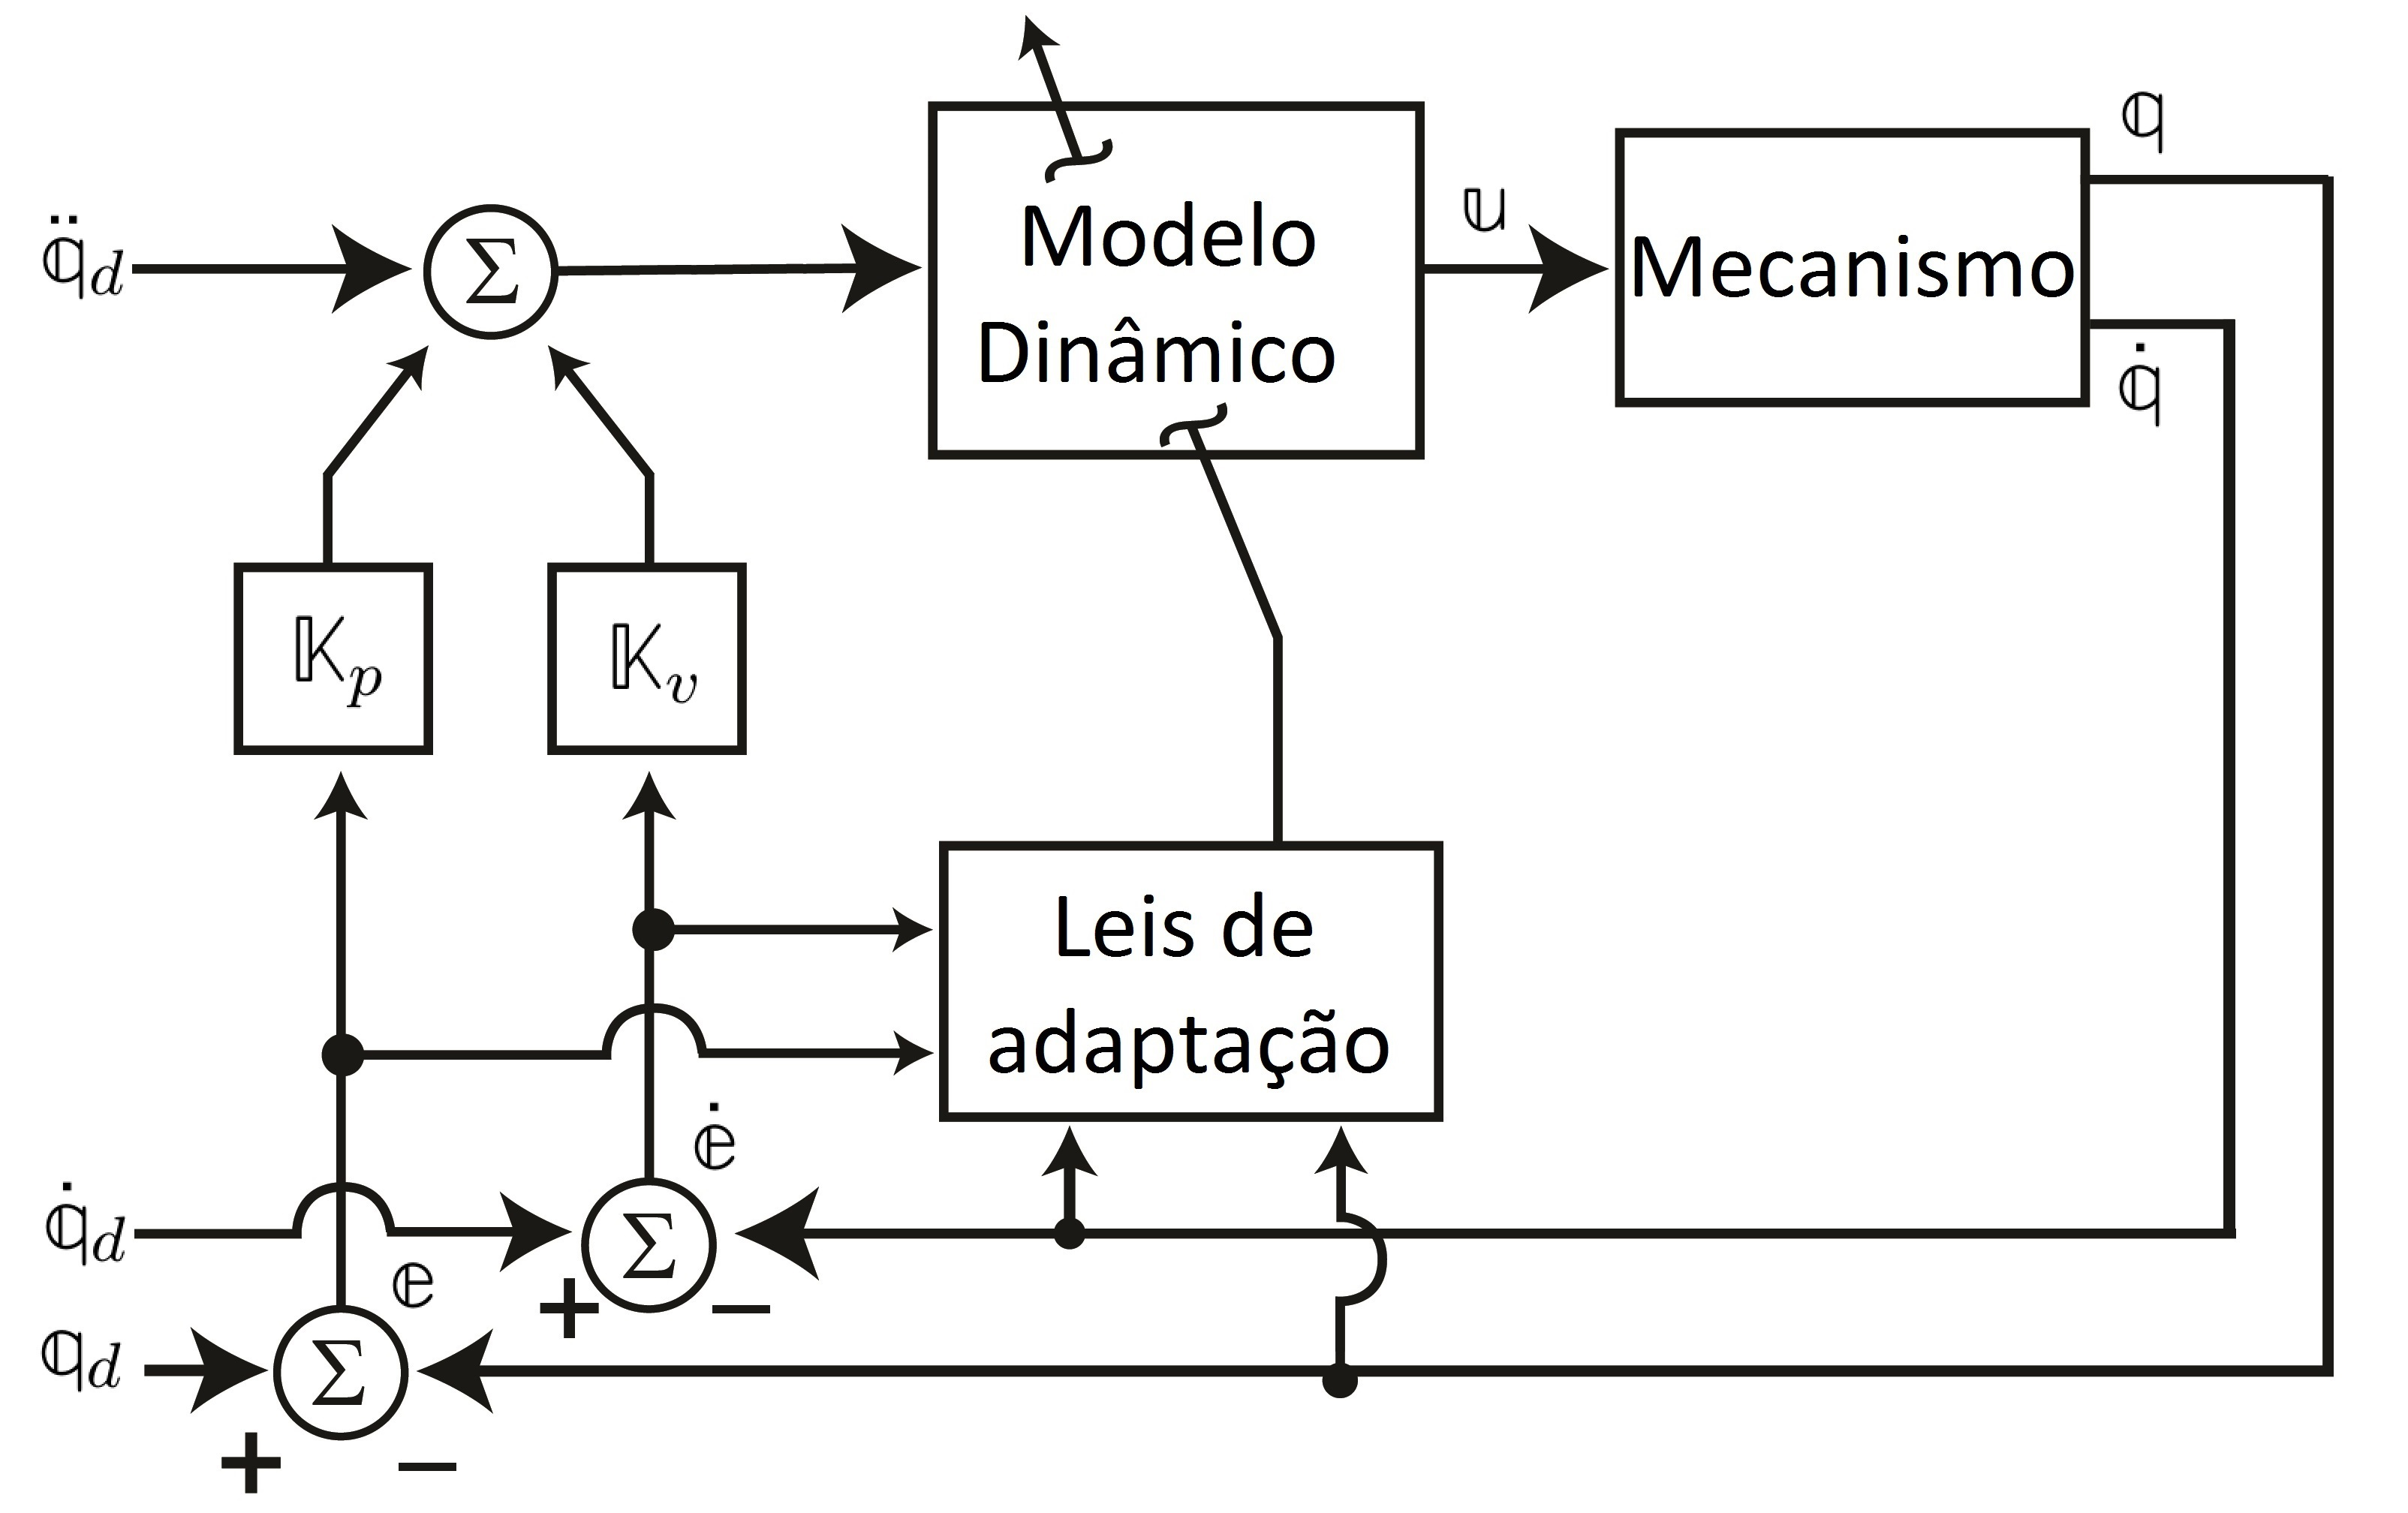
\includegraphics[scale=0.47]{../figures/CA.jpg}  
	\caption{Malha de Controle Adaptativo (Adaptado de \cite{Craig})}
	\label{fig:CA}
\end{figure}

\subsection{Controle por Modos Deslizantes (MD)}

Outra técnica promissora para aplicação em mecanismos paralelos é o Controle por Modos Deslizantes (MD). A técnica consiste no projeto de leis de controle que levem o sistema para superfícies de escorregamento no espaço de fase, de modo que assim que o sistema atinje e é mantido nas superfícies de escorregamento, o erro de controle decai exponencialmente para zero \cite{Slotini}. Para garantir que o sistema atinja em tempo finito e se mantenha nas superfícies de escorregamento, são utilizados termos descontínuos na lei de controle, o que pode causar problemas de oscilações bruscas em alta frequência nos esforços de controle ({\em chattering}). Em \cite{Guldner}  e  \cite{Utkin2} são propostas técnicas para evitar esse tipo de problema. A grande vantagem da utilização deste tipo de lei de controle é sua grande robustez a incertezas estruturadas e não estruturadas, sendo possível realizar o projeto do controlador de modo a suprimir um dado nível de incertezas paramétricas. Em \cite{SlotiniSMC} é proposta uma metodologia de projeto de Controle por Modos Deslizantes para manipuladores robóticos seriais. A figura \ref{fig:CMD} mostra um diagrama de blocos típico de MD aplicado a sistemas mecânicos. 

Na literatura são encontradas diversos artigos utilizando a técnica de MD aliada à lógica {\em fuzzy} e/ou redes neurais para o controle de manipuladores robóticos \cite{Begon, Ertugrul, Hu, Sadati}. Begon \emph{et al.} \cite{Begon} propuseram uma lei de controle baseada na teoria de MD e na utilização de lógica {\em fuzzy} para controlar de maneira independente os atuadores de um mecanismo paralelo do tipo Hexa. A técnica proposta teve o intuito de obter a robustez característica do MD sem necessitar de uma lei de controle com termos descontínuos, evitando o {\em chattering}.

Em \cite{Zeinali}, Zeinali \emph{et al.} desenvolveram uma lei de controle  baseada nas teorias de MD e Controle Adaptativo. O controlador desenvolvido realiza a compensação dinâmica em tempo real do erro de modelagem através de uma lei de adaptação. Além disso, substitui o termo descontínuo da lei de controle por um termo do tipo PID, com o intuito de evitar o {\em chattering}. A estabilidade e robustez da lei de controle proposta foram provadas utilizando a teoria de estabilidade de Lyapunov \cite{Slotini}. A robustez da lei de controle foi verificada através de simulações do controlador proposto aplicado a um mecanismo serial do tipo \underline{R}\underline{R}, nas quais o controlador conseguiu manter erros de posição muito pequenos em regime permanente, mesmo sendo baseado em um modelo muito pobre e na presença de distúrbios de torque. A técnica apresentada se mostra promissora, porém, como no artigo foi feita apenas a simulação da lei de controle em um mecanismo serial bidimensional, ainda não se pode afirmar nada sobre seu desempenho em mecanismos paralelos tridimensionais.

\begin{figure}[h]
	\centering
	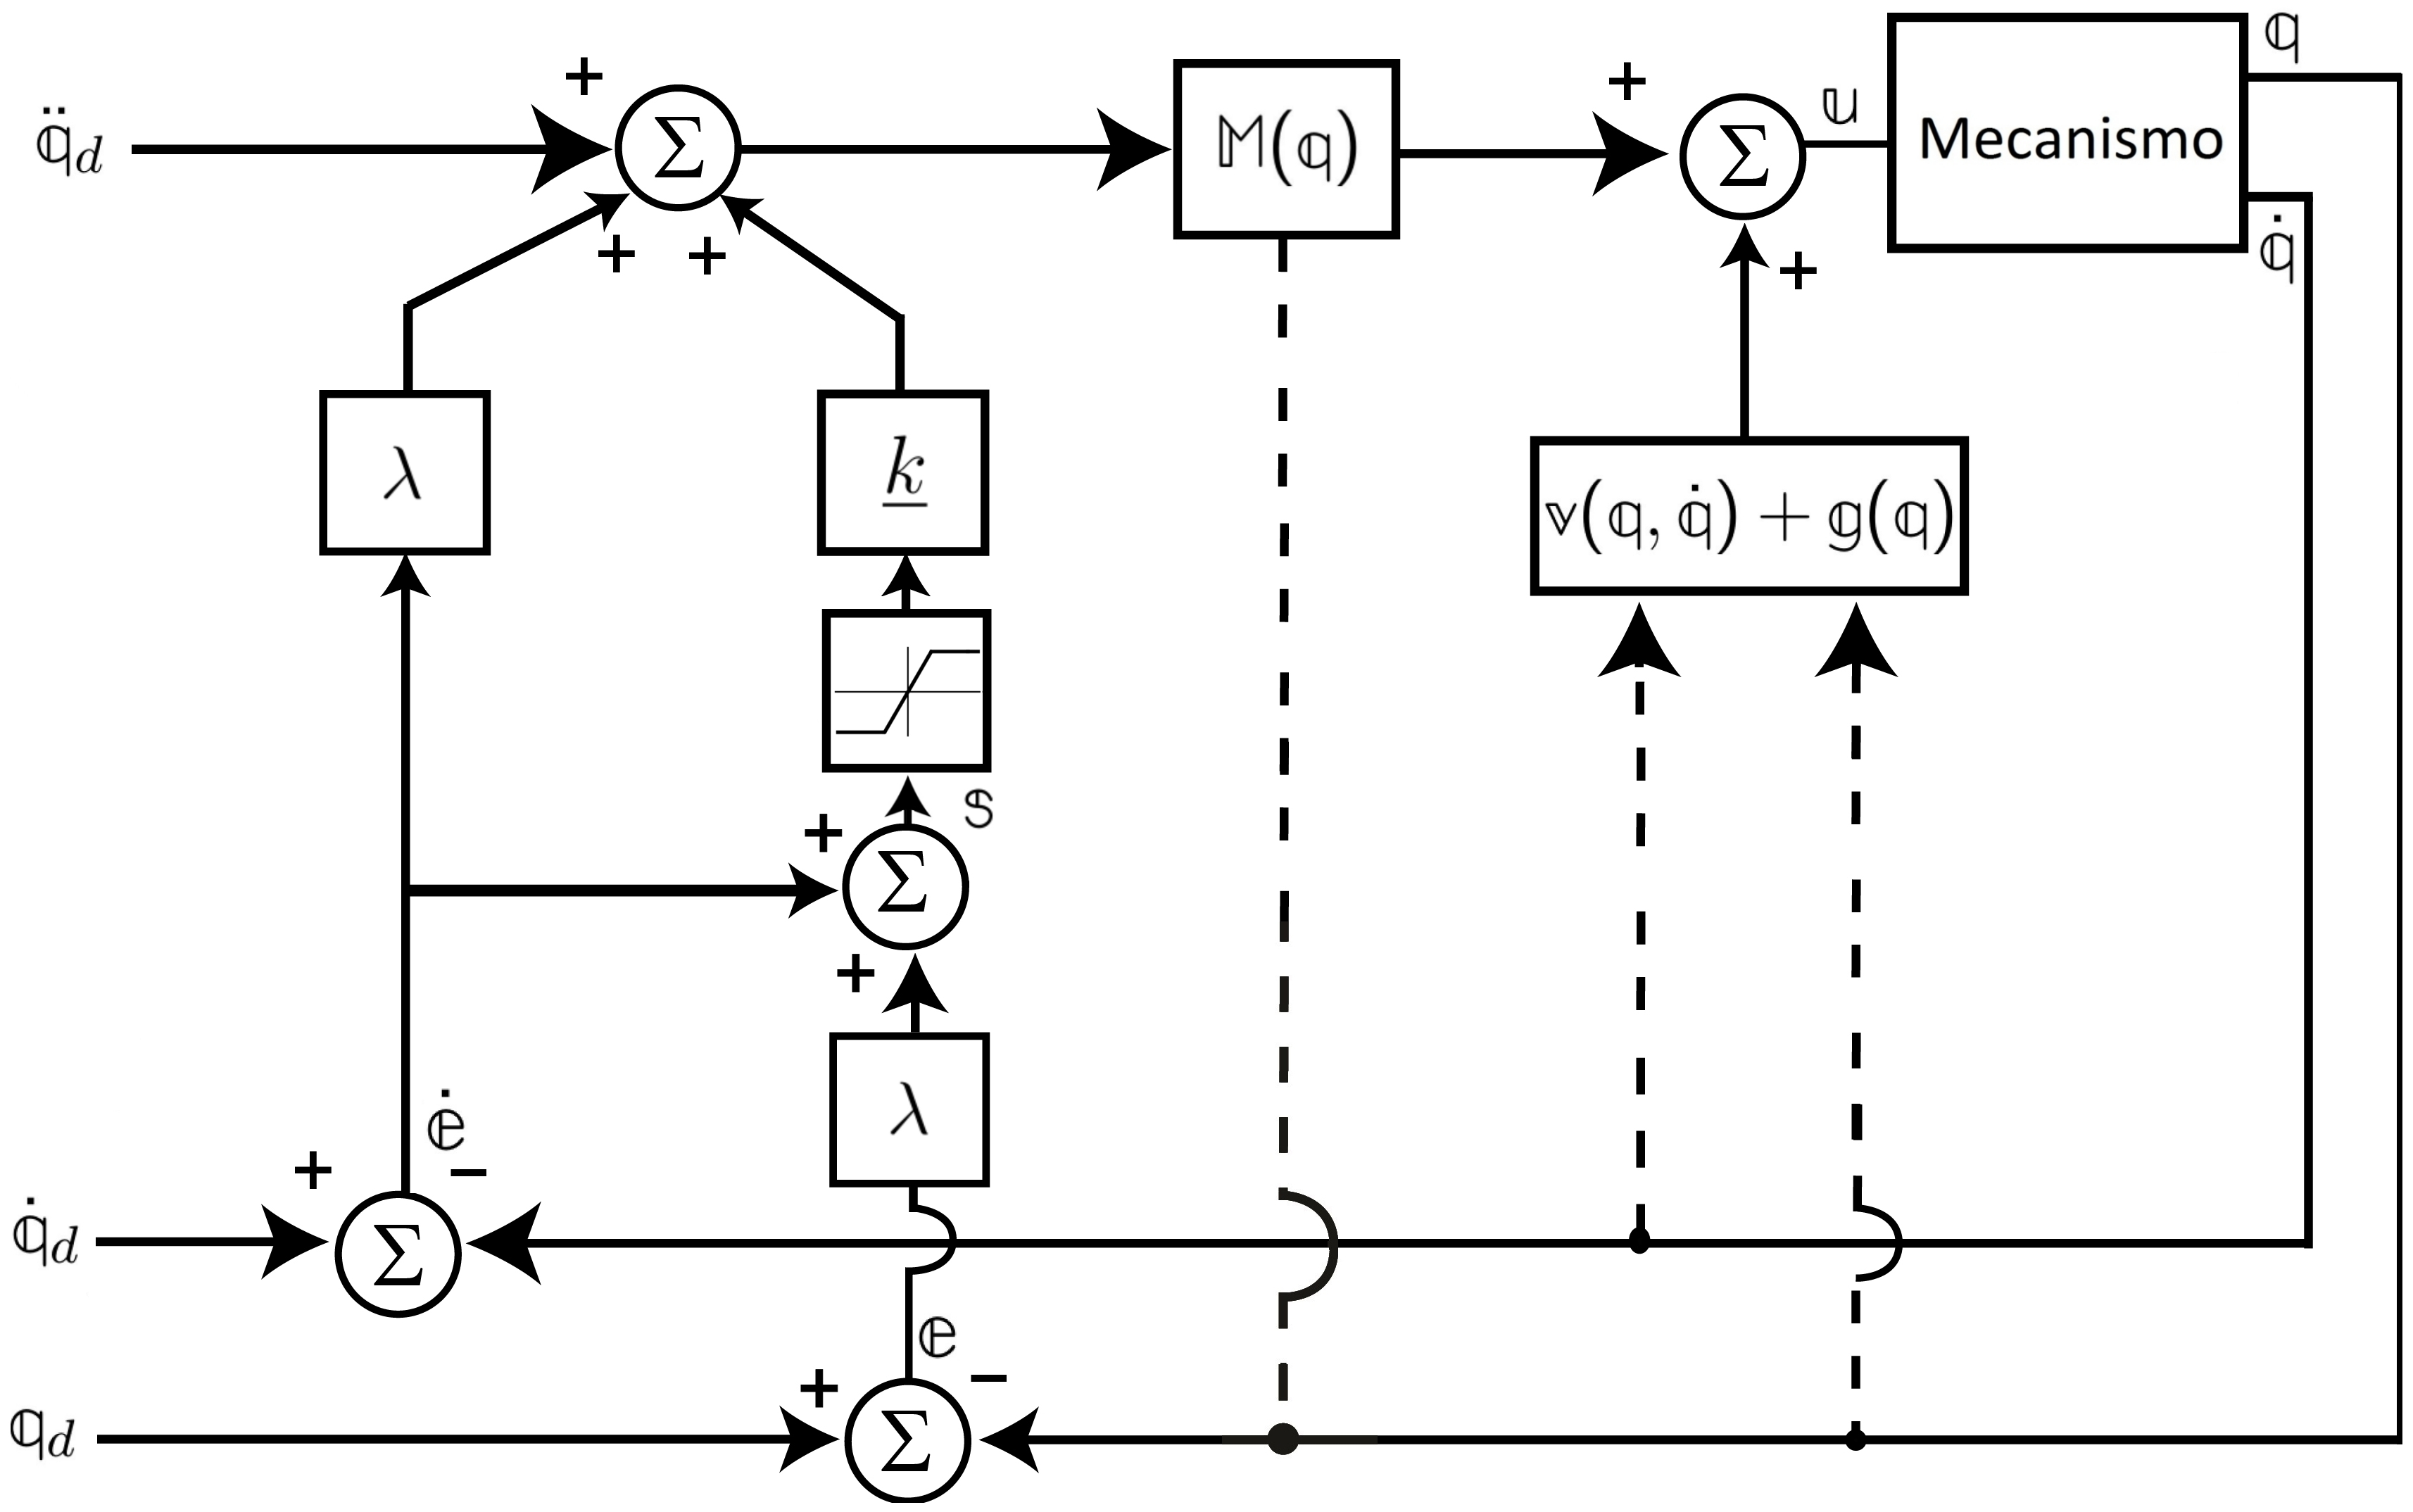
\includegraphics[scale=0.55]{../figures/CMD.jpg}  
	\caption{Malha Controle por Modos Deslizantes}
	\label{fig:CMD}
\end{figure}

\section{Conclusões}

Após a realização das revisões da literatura relativas à modelagem dinâmica e ao controle de mecanismos paralelos, é possível perceber alguns fatos que valem a pena ser comentados.

Primeiramente, em relação à modelagem dinâmica, em boa parte dos trabalhos, a modelagem é realizada de uma maneira um tanto quanto ineficiente, tanto no sentido do trabalho necessário para realizar a dedução, quanto na parte da implementação, como é o caso dos artigos citados que utilizam o formalismo de Newton-Euler. 

Por outro lado, há artigos que propõe formulações que se mostram muito eficientes no processo de modelagem, as quais se utilizam de artifícios de modularidade e/ou recursividade, como os trabalhos citados baseados na formulação do Complemento Ortogonal Natural. No entanto, praticamente todas essas formulações necessitam do cálculo de derivadas de jacobianos de maneira simbólica, o que dificulta muito o processo de automatização desses métodos. Além disso, conforme a complexidade dos mecanismos aumenta, essas derivadas tendem a gerar expressões maiores e mais complexas.

Também não foram encontrados trabalhos que propõe um conjunto de parâmetros que definam a arquitetura de pelo menos uma classe de mecanismos paralelos, análogos aos parâmetros de Denavit-Hartemberg para os mecanismos seriais \cite{Denavit}.

Com relação à revisão das técnicas de controle aplicadas a mecanismos paralelos, foi possível perceber que, apesar de até que uma boa parte apresentar resultados experimentais \cite{Honegger, Cheng, Shang, Yen, Codourey, Vivas, Duchaine, Chemori, Begon}, são poucos os que realmente apresentam uma análise um pouco mais elaborada. Além disso, há menos trabalhos experimentais que mostram a eficácia de técnicas que podem superar ou bater de frente com o Controle por Torque Computado. Também não foram encontrados trabalhos que tratam da questão da implementação de técnicas de controle baseado em modelo e da questão de como reduzir seu custo computacional.

Sendo assim, com relação à modelagem dinâmica, esta Tese visa contribuir através do desenvolvimento de um algoritmo genérico para a modelagem dinâmica de mecanismos paralelos translacionais que: utiliza estratégias modulares; não necessita do cálculo simbólico de derivadas; e propõe uma maneira de descrever a topologia deste tipo de mecanismo utilizando um conjunto de parâmetros.

Em relação ao controle, esta tese visa contruir através da proposição de novas leis de controle híbridas, as quais adicionam termos de controle robusto a técnicas de controle já bastante populares na literatura, e da comprovação experimental da eficácia das técnicas propostas no controle de mecanismos paralelos.

%METODOLOGIA--------------------------------------------------------------------
\chapter{Metodologia da Pesquisa}\label{method}

Fundamentalmente, a metodologia desta pesquisa compreende a execução de seis fases, abrangendo desde o desenvolvimento de algoritmos para as modelagens cinemática e dinâmica ao projeto de controladores e sua validação experimental.

\section{Primeira fase} 
Desenvolver um algoritmo genérico, capaz de gerar os modelos dinâmicos completos de mecanismos paralelos translacionais que operem em espaço plano ou tridimensional. Esta geração parte da definição da topologia do mecanismo paralelo, suas cadeias cinemáticas, descrevendo a localização relativa de seus elos e juntas. 

Dentre os efeitos de modelagem considerados, destacam-se os decorrentes da inércia efetiva e acoplada, das forças de Coriolis e centrífugas, da força gravitacional, bem como dos esforços dos atuadores. Pretende-se que a geração dos modelos seja realizada de forma implícita. Para tanto, será desenvolvida uma metodologia baseada no método Recursivo Modular de Modelagem (RMM) proposto por Orsino \cite{23orsino} que, por meio da definição de níveis hierárquicos da estrutura de um sistema mecânico e a descrição da dependência das variáveis cinemáticas envolvidas,  permite o acoplamento de subsistemas multicorpos.

\section{Segunda fase} 
Efetuar as modelagens cinemática e dinâmica do mecanismo articulado plano 5R \cite{22orsino}, utilizando o algoritmo desenvolvido na fase anterior.

\section{Terceira fase} 
Nesta fase, diferentes técnicas de controle serão avaliadas sob a perspectiva de sua utilização em manipuladores paralelos. Assim, em princípio, esta pesquisa foca na síntese de um controlador não-linear robusto e de alto desempenho. Para tanto, serão consideradas as incertezas paramétricas e a possibilidade de atuação redundante \cite{Cheng}, além de estratégias para a determinação de leis de controle com custo computacional consideralvemente menor do que as tradicionais, que empreguem o Controle por Torque Computado \cite{Craig, Zubizarreta}.

\section{Quarta fase} Avaliar o emprego de diferentes técnicas de controle de trajetória aplicadas especificamente para o manipulador 5R, empregando a metodologia da terceira fase.

\section{Quinta fase} Realizar diversas simulações que permitam observar a consistência dos resultados, no tocante às análises cinemáticas direta e inversa, bem como das análises dinâmicas direta e inversa. Além disso, serão determinadas as respostas dinâmicas do manipulador sujeito às distintas leis de controle sintetizadas.

\section{Sexta fase} 
De modo a avaliar o desempenho previsto pelo uso de diferentes controladores para o manipulador paralelo 5R (figura \ref{fig:Clara}), será realizada a validação experimental em uma das bancadas de ensaio do LaMMaR. Para tanto, serão escolhidas duas trajetórias: uma que considere o comportamento em regime permanente e outra em regime transitório. 

Neste sentido, almeja-se observar se haverá alguma diferença de desempenho se o controle for executado no espaço das juntas ou no da tarefa. Além disso, pretende-se considerar os efeitos da implementação de técnicas de controle puras ou combinadas. Para auxiliar na comparação entre as técnicas de controle, serão definidas duas métricas: uma que considere o erro de posicionamento do efetuador e outra a magnitude dos torques dos atuadores.

%\section{O que tinha antes} 
%O estágio atual de desenvolvimento do presente projeto ocorre basicamente em três áreas:
%aplicação do algoritmo de modelagem e simulação para os mecanismos 5R \cite{22orsino} e 2\underline{R}SU + \underline{P}PaP \cite{Kumazawa}, o projeto e simulação de controladores não lineares robustos de alto desempenho baseado no modelo dinâmico para os mecanismos citados, e a validação experimental das leis de controle sintetizadas.

%Os trabalhos no âmbito de modelagem e simulação estão sendo desenvolvidos a partir da aplicação do algoritmo de modelagem cinemática e dinâmica de mecanismos paralelos desenvolvido, baseado na utilização dos parâmetros de Denavit-Hartenberg \cite{Craig, Denavit, Lipkin} e no método Orsino de acoplamento de subsistemas \cite{23orsino}. Toda modelagem será feita em C++, utilizando uma biblioteca otimizada de cálculo matricial (Armadillo).
%As simulações da dinâmica direta do mecanismo serão feitas utilizando o método Runge-Kutta de 8ª ordem \cite{RK} para solução de sistemas de EDOs, de modo a garantir estabilidade numérica do método, mesmo utilizando leis de controle quase descontínuas.

%Os trabalhos na área de projeto de controle serão feitos utilizando a metodologia desenvolvida de projeto de controladores robustos multivariáveis para mecanismos paralelos, baseada no modelo dinâmico do mecanismo a ser controlado e na técnica de controle por modos deslizantes \cite{Slotini, Utkin}.

%Os trabalhos no âmbito da validação experimental das leis de controle sintetizadas serão realizados no protótipo do mecanismo 5R que encontra-se no laboratório de mecanismos. A bancada experimental do mecanismo 5R já está funcional e já forem realizados alguns testes de leis de controle de trajetória baseadas no modelo dinâmico do mecanismo. Para a realização da validação experimental nesta bancada, será realizada a identificação dos parâmetros do sistema e suas respectivas incertezas, projeto do controlador baseado nos parâmetros e incertezas identificadas, implementação das leis de controle, e aquisição de dados. \\

\begin{figure}[h]
	\centering
	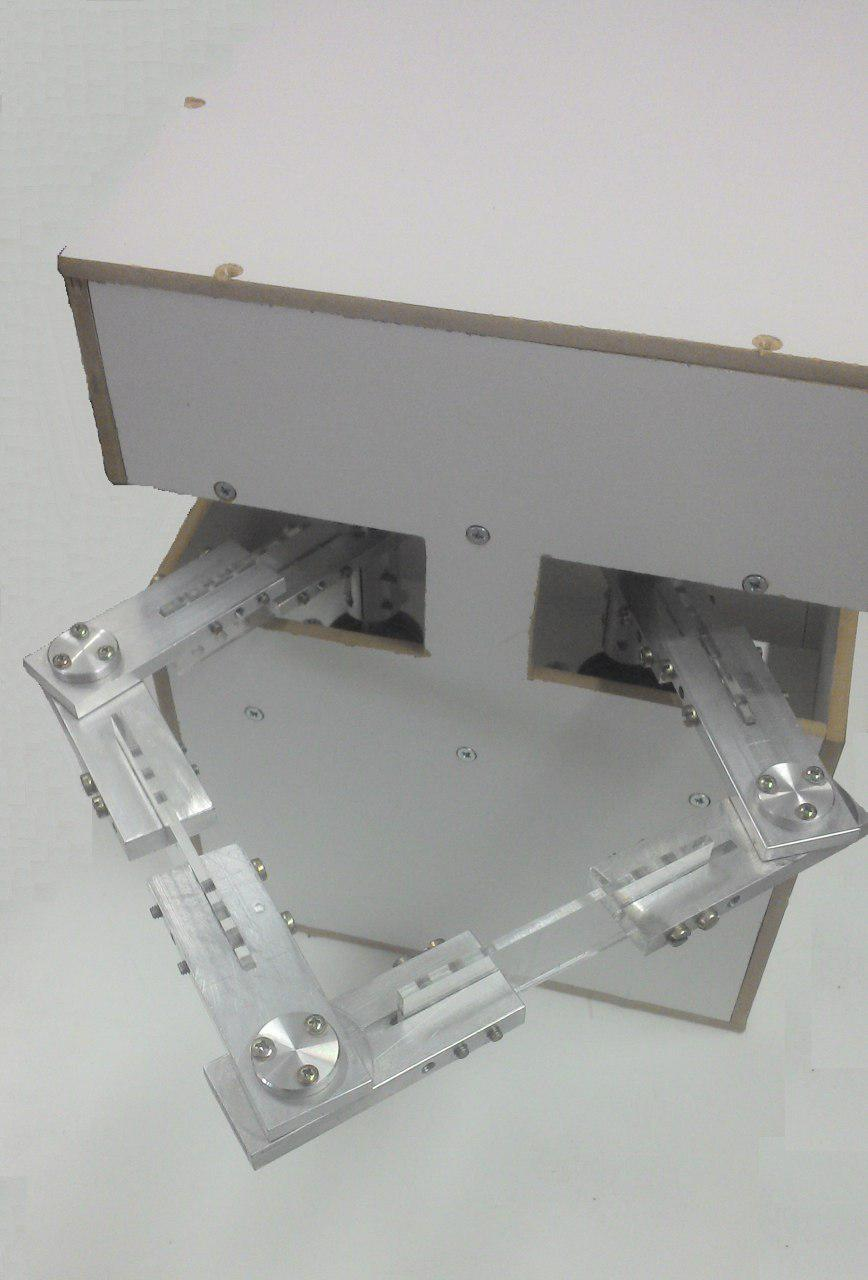
\includegraphics[scale=0.3]{../figures/Clara.jpg}  
	\caption{Protótipo do mecanismo 5R}
	\label{fig:Clara}
\end{figure}

%MODELAGEM DE MANIPULADORES SERIAIS--------------------------------------------

\part{Modelagem e Controle}
	
\chapter{Modelagem de manipuladores seriais} \label{cap:Seriais}
\capepigrafe[0.5\textwidth]{``Não é que eu goste de complicar as coisas, elas é que gostam de ser complicadas comigo''}{Lewis Carroll}

Este capítulo tem o intuito de apresentar um algoritmo genérico para a obtenção do modelo cinemático e dinâmico de mecanismos seriais. O algoritmo apresentado é implementável em linguagens de programação comumente usadas atualmente, como C++, Java e Python, sem necessitar de recursos de manipulação simbólica. \\
Para a obtenção do modelo, são necessários apenas os parametros de Denavit-Hartemberg \cite{Craig, Denavit, Lipkin, Cabral} do mecanismo e as posições dos centros de massa dos ligamentos em relação aos sistemas de coordenadas fixos aos ligamentos. \\ 

Seja $\ssB$ um sistema mecânico serial de $\nu$ graus de liberdade. Primeiramente, fazemos as seguintes definições:

\begin{itemize}
\item $\llN$ ou $\llB_0$: referencial inercial.
\item $\ttN$ ou $\ttB_0$: sistema de coordenadas da base do mecanismo, fixo a $\llN$.
\item $\llB_i, \,i=1,...,\nu$: i-ésimo ligamento.
\item $\ttB_i, \,i=1,...,\nu$: sistema de coordenadas solidário a $\llB_i$.
%\item $\tto_i, \,i=0,...,\nu$: origem do sistema $\ttB_i$.
%\item $\{\vi_i, \vj_i, \vk_i\}, \,i=0,...,\nu$: base ortonormal do sistema $\ttB_i$.
\item $\ttc_{\lllB_i}, \,i=1,...,\nu$: centro de massa do ligamento $\llB_i$.
\item $\ttx$: ponto no espaço fixo ao efetuador.
\item $\ttX$: sistema de coordenadas fixo ao efetuador, com origem em $\ttx$ e a mesma base de $\ttB_\nu$. 
\item $m_i$: massa do ligamento $\llB_i$.
%\item $\vI_{\lllB_i}$: tensor de in\'ercia do ligamento $\llB_i$ em relação a seu centro de massa.
\item $\mI_i$: tensor de in\'ercia $\vI_{\lllB_i}$ escrito na base $\ttN$, ou seja, $\vct{\vI_{\lllB_i}}_{\ttN \rl \ttN}$.
\item $\mI'_i$: tensor de in\'ercia $\vI_{\lllB_i}$ escrito na base $\ttB_i$, ou seja, $\vct{\vI_{\lllB_i}}_{\ttB_i \rl \ttB_i}$.
\item $q_i, \,i=1,...,\nu$: deslocamento relativo (angular ou linear) da i-ésima junta.
\item  $\mq$: matriz-coluna de $\nu$ coordenadas generalizadas independentes. É dada por $\mq = \begin{bmatrix}
q_1 & ... & {q}_{\nu}
\end{bmatrix}^\msT $.
%\item $\vg$: Vetor aceleração gravitacional.
\item $\mgamma$: vetor aceleração gravitacional escrito na base $\ttN$, ou seja, $\vct{\vgamma}_{\ttN}$.
%\item $\vf_i$: Vetor força não-reativa resultante aplicada no centro de massa de $\llB_i$.
%\item $\vtau_i$: Vetor torque não-reativo resultante aplicado em $\llB_i$.
\item $\overline{\mf}_i$: matriz-coluna de esforços não-reativos generalizados aplicados ao subsistema $\llB_i$. É dada por $\overline{\mf}_i = \begin{bmatrix}
\vct{\vf_{\lllB_i}}_\ttN^\msT &
\vct{\vtau_{\lllB_i}}_\ttN^\msT
\end{bmatrix}^\msT $.
\item $\mR_i, \,i=1, ..., \nu$: matriz de rotação $\vct{\vone}_{\ttN \rl \ttB_i}$.
\item $\mR'_i, \,i=1, ..., \nu$: matriz de rotação $\vct{\vone}_{\ttB_{i-1} \rl \ttB_i}$.
%\item $\mX$: matriz de rotação $\vct{\vone}_{\ttN \rl \ttX}$.
\item $\breve{\mr}_i, \,i=1, ..., \nu$: representação via quaternion unitário da matriz de rotação $\vct{\vone}_{\ttN \rl \ttB_i}$.
\item $\breve{\mr}'_i, \,i=1, ..., \nu$: representação via quaternion unitário da matriz de rotação $\vct{\vone}_{\ttB_{i-1} \rl \ttB_i}$.
\item $\breve{\mx}, \,i=1, ..., \nu$: representação via quaternion unitário da matriz de rotação $\vct{\vone}_{\ttN \rl \ttX}$.
\item $\mo_i, \,i=0, ..., \nu$: origem $\tto_{\ttB_i}$ no sistema de coordenadas $\ttN$, ou seja $\vct{\tto_{\ttB_i}}_\ttN$.
\item $\mo'_i, \,i=1, ..., \nu$: origem $\tto_{\ttB_i}$ no sistema de coordenadas $\ttB_{i-1}$, ou seja $\vct{\tto_{\ttB_i}}_{\ttB_{i-1}}$.
\item $\mx, \,i=1, ..., \nu$: ponto $\ttx$ no sistema de coordenadas $\ttN$, ou seja $\vct{\ttx}_\ttN$.
\item $\mc_{\cM\,i}, \,i=1, ..., \nu$: centro de massa $\ttc_{\lllB_i}$ no sistema de coordenadas $\ttN$, ou seja $\vct{\ttc_{\lllB_i}}_\ttN$.
\item $\mc'_{\cM\,i}, \,i=1, ..., \nu$: centro de massa $\ttc_{\lllB_i}$ no sistema de coordenadas $\ttB_{i}$, ou seja $\vct{\ttc_{\lllB_i}}_{\ttB_{i}}$.
\item $\mk_i, \,i=0, ..., \nu$: componentes do versor $\vk_{\ttB_i}$ no sistema de coordenadas $\ttN$, ou seja $[\vk_{\ttB_i}]_\ttN$.
\item $\momega_i, \,i=1, ..., \nu$: componentes de velocidade angular do ligamento $\llB_i$ em relação ao referencial $\llN$ no sistema $\ttN$, ou seja $\vct{\vomega_{\lllB_i}^{\lllN}}_\ttN$.
\item $\momega'_i, \,i=1, ..., \nu$: componentes de velocidade angular do ligamento $\llB_i$ em relação ao referencial $\llB_{i-1}$ no sistema $\ttN$, ou seja $\vct{\vomega_{\lllB_i}^{\lllB_{i-1}}}_\ttN$.
\item $\momega$: componentes de velocidade angular do efetuador em relação ao referencial $\llN$ no sistema $\ttN$, ou seja $\vct{\vomega_{\lllB_\nu}^{\lllN}}_\ttN$.
\item $\mv_i, \,i=1, ..., \nu$: componentes de velocidade do centro de massa do ligamento $\llB_i$ em relação ao referencial $\llN$ no sistema $\ttN$, ou seja $\vct{\vv_{\ttc_{\lllB_i}}^{\lllN}}_\ttN$.
\item $\mv'_i, \,i=1, ..., \nu$: componentes de velocidade do centro de massa do ligamento $\llB_i$ em relação ao referencial $\llB_{i-1}$ no sistema $\ttN$, ou seja $\vct{\vv_{\ttc_{\lllB_i}}^{\lllB_{i-1}}}_\ttN$.
\item $\mv$: componentes de velocidade do efetuador em relação ao referencial $\llN$ no sistema $\ttN$, ou seja $\vct{\vv_{\ttx}^{\lllN}}_\ttN$.
\item $\malpha_i, \,i=1, ..., \nu$: componentes de aceleração angular do ligamento $\llB_i$ em relação ao referencial $\llN$ no sistema $\ttN$, ou seja $\vct{\valpha_{\lllB_i}^{\lllN}}_\ttN$.
\item $\malpha'_i, \,i=1, ..., \nu$: componentes de aceleração angular do ligamento $\llB_i$ em relação ao referencial $\llB_{i-1}$ no sistema $\ttN$, ou seja $\vct{\valpha_{\lllB_i}^{\lllB_{i-1}}}_\ttN$.
\item $\malpha$: componentes de aceleração angular do efetuador em relação ao referencial $\llN$ no sistema $\ttN$, ou seja $\vct{\valpha_{\lllB_\nu}^{\lllN}}_\ttN$.
\item $\ma_i, \,i=1, ..., \nu$: componentes de aceleração do centro de massa do ligamento $\llB_i$ em relação ao referencial $\llN$ no sistema $\ttN$, ou seja $\vct{\va_{\ttc_{\lllB_i}}^{\lllN}}_\ttN$.
\item $\ma'_i, \,i=1, ..., \nu$: componentes de aceleração do centro de massa do ligamento $\llB_i$ em relação ao referencial $\llB_{i-1}$ no sistema $\ttN$, ou seja $\vct{\va_{\ttc_{\lllB_i}}^{\lllB_{i-1}}}_\ttN$.
\item $\ma$: componentes de aceleração do efetuador em relação ao referencial $\llN$ no sistema $\ttN$, ou seja $\vct{\va_{\ttx}^{\lllN}}_\ttN$.
\item $\mu$: matriz-coluna dos esforços ativos generalizados aplicados pelos atuadores das juntas.
\end{itemize}

Para facilitar a leitura das equações, nas expressões que envolvem o indice $i$, estará subentendido que $i$ varia de $1$ a $\nu$, ou seja, $i=1,\hdots,\nu$, a menos que seja explicitado de forma diferente. A dependência das variáveis, indicada por parênteses, também será omitida em algumas equações para facilitar a leitura.

Algumas equações serão destacadas através de cores. A cor amarela indica equações que devem ser implementadas no algoritmo. A cor azul escura indica equações de destaque no desenvolvimento. A cor azul clara indica equações de destaque secundário no desenvolvimento.

\section{Cinemática}

\subsection{Cinemática de posição}

Dados os parâmetros de Denavit-Hartemberg $a_i$, $\alpha_i$, $d_i$ e $\theta_i$, com $i=1,\hdots,\nu$, é possível obter as matrizes de transformação homogênea $\hvct{\vone}_{\ttB_{i-1} \rl \ttB_i}$ a partir da seguinte expressão \cite{Cabral}:
\begin{equation} \label{eq:TransformacaoHomogeneaDH}
\hvct{\vone}_{\ttB_{i-1} \rl \ttB_i} =
\begin{bmatrix}
\ccos\theta_i & -\ssin\theta_i \ccos\alpha_i &  \ssin\theta_i \ssin\alpha_i & a_i\ccos\theta_i \\
\ssin\theta_i &  \ccos\theta_i \ccos\alpha_i & -\ccos\theta_i \ssin\alpha_i & a_i\ssin\theta_i \\
0             &  \ssin\alpha_i               &  \ccos\alpha_i               & d_i \\
0             & 0                            & 0                            & 1
\end{bmatrix}
\end{equation}

Logo:
\begin{empheq}[box=\lightbluebox]{equation}
\mR'_i(q_i) = \vct{\vone}_{\ttB_{i-1} \rl \ttB_i} =
\begin{bmatrix}
\ccos\theta_i & -\ssin\theta_i \ccos\alpha_i &  \ssin\theta_i \ssin\alpha_i \\
\ssin\theta_i &  \ccos\theta_i \ccos\alpha_i & -\ccos\theta_i \ssin\alpha_i \\
0             &  \ssin\alpha_i               &  \ccos\alpha_i
\end{bmatrix}
\end{empheq}

\begin{empheq}[box=\myyellowbox]{equation}
\mo'_i(q_i) = \vct{\tto_{\ttB_i}}_{\ttB_{i-1}} =
\begin{bmatrix}
a_i\ccos\theta_i &
a_i\ssin\theta_i &
d_i
\end{bmatrix}^\msT
\end{empheq}

A cinemática de posição do efetuador poderia ser feita a partir da composição (produtos) de matrizes de transformação homogênea. Este tipo de estratégia é bastante conveniente quando se trata da realização de cálculos simbólicos. Entretanto, não é muito adequada para implementações numéricas, devido ao acúmulo de erros numéricos gerado pela multiplicação de matrizes de rotação.

Uma representação de rotação por quaterion unitário equivalente à matriz $\mR'_i(q_i)$ é dada por:
\begin{empheq}[box=\myyellowbox]{equation}
\breve{\mr}'_i(q_i) =
\begin{bmatrix}
\sign(\ssin \alpha_i) \sqrt{(1+\ccos \theta_i)(1-\ccos \alpha_i)}/2 \\
\sign(\ssin \theta_i \ssin \alpha_i) \sqrt{(1-\ccos \theta_i)(1-\ccos \alpha_i)}/2 \\
\sign(\ssin \theta_i) \sqrt{(1-\ccos \theta_i)(1+\ccos \alpha_i)}/2 \\
\sqrt{(1+\ccos \theta_i)(1+\ccos \alpha_i)}/2
\end{bmatrix}
\end{empheq}

Para solucionar este paradigma, as composições de rotações e translações serão feitas separadamente, sendo que a composição de rotações será feita atravez da multiplicação de quaternions unitários. 

Tendo obtido $\vct{\vone}_{\ttB_{i-1} \rl \ttB_i}$, seria possível obter as matrizes de rotação que relacionam os sistemas de coordenadas solidários aos ligamentos ($\ttB_i$) ao sistema de coordenadas da base ($\ttN$) pela seguinte expressão recursiva:
\begin{equation} \label{eq:H__}
\begin{split}
\vct{\vone}_{\ttN \rl \ttB_i} =
\begin{cases}
\vct{\vone}_{\ttB_0 \rl \ttB_1}, & \text{se } i=1 \\
\vct{\vone}_{\ttN \rl \ttB_{i-1}} \cdot \vct{\vone}_{\ttB_{i-1} \rl \ttB_i}  , & \text{se } i>1
\end{cases}
\end{split}
\end{equation}

Ou seja
\begin{equation}
\begin{split}
\mR_i(\mq) =
\begin{cases}
\mR'_1(q_1), & \text{se } i=1 \\
\mR_{i-1}(\mq) \cdot \mR'_i(q_i), & \text{se } i>1
\end{cases}
\end{split}
\end{equation}

A composição de rotações utilizando quaternions unitários é obtida através de uma expressão análoga:
\begin{empheq}[box=\myyellowbox]{equation}
\begin{split}
\breve{\mr}_i(\mq) =
\begin{cases}
\breve{\mr}'_1(q_1), & \text{se } i=1 \\
\breve{\mr}_{i-1}(\mq) \otimes \breve{\mr}'_i(q_i), & \text{se } i>1
\end{cases}
\end{split}
\end{empheq}

Para evitar o acúmulo de erros numéricos, basta renormalizar cada quaternion obtido através do produto de dois outros.

As expressões das matrizes de rotação $\mR_i(\mq)$ podem ser obtidas através da fórmula de conversão de quaternions unitários para matrizes de rotação apresentada no apêndice \ref{ap:Quat}.
\begin{equation} \tag{\ref{eq:Quat2Matriz}}
\mR = \underline{\mR}(\breve{\mq}) = \begin{bmatrix}
1 - 2 q_j^2 - 2 q_k^2 & 2(q_i q_j - q_k q_r) & 2(q_i q_k + q_j q_r) \\
2(q_i q_j + q_k q_r) & 1 - 2 q_i^2 - 2q_k^2 & 2(q_j q_k - q_i q_r) \\
2(q_i q_k - q_j q_r) & 2(q_i q_r + q_j q_k) & 1 - 2 q_i^2 - 2 q_j^2
\end{bmatrix}
\end{equation}

\begin{empheq}[box=\myyellowbox]{equation}
\mR_i(\mq) = \underline{\mR}(\breve{\mr}_i(\mq))
\end{empheq}

A composição de translações pode ser feita da seguinte maneira:
\begin{equation}
\begin{split}
\vct{\tto_{\ttB_i}}_{\ttN} =
\begin{cases}
\vct{\tto_{\ttB_1}}_{\ttB_0}, & \text{se } i=1 \\
\vct{\tto_{\ttB_{i-1}}}_{\ttN} +  \vct{\vone}_{\ttN \rl \ttB_{i-1}} \cdot \vct{\tto_{\ttB_i}}_{\ttB_{i-1}}   , & \text{se } i>1
\end{cases}
\end{split}
\end{equation}

Tendo em vista que $\mo_0 = \vct{\tto_{\ttB_0}}_{\ttB_0} = \mzr$, temos que:
\begin{empheq}[box=\myyellowbox]{equation}
\begin{split}
\mo_i(\mq) =
\begin{cases}
\mzr, & \text{se } i=0 \\
\mo'_1(q_1), & \text{se } i=1 \\
\mo_{i-1}(\mq) +  \mR_{i-1}(\mq) \cdot \mo'_i(q_i)   , & \text{se } i>1
\end{cases} \; i=0,...,\nu
\end{split}
\end{empheq}

Sendo assim,  a posição do efetuador no sistema $\ttN$ e a representação por quaternion da orientação do efetuador são dadas por:
\begin{empheq}[box=\myyellowbox]{equation}
\mx(\mq) = \mo_\nu (\mq)
\end{empheq}
\begin{empheq}[box=\myyellowbox]{equation}
\breve{\mx}(\mq) = \breve{\mr}_\nu (\mq)
\end{empheq}
%\begin{empheq}[box=\myyellowbox]{equation}
%\mX(\mq) = \mR_\nu (\mq)
%\end{empheq}

Tendo obtidos as matrizes de rotação $\vct{\vone}_{\ttN \rl \ttB_i}$ e as coordenadas das origens $\tto_{\ttB_i}$ no sistema $\ttN$,  temos que as coordenadas dos centros de massa dos ligamentos são dadas por:
\begin{equation}
\vct{\ttc_{\lllB_i}}_{\ttN} = \vct{\tto_{\ttB_i}}_{\ttN} + \vct{\vone}_{\ttN \rl \ttB_i} \cdot \vct{\ttc_{\lllB_i}}_{\ttB_i}
\end{equation}

Ou seja
\begin{empheq}[box=\myyellowbox]{equation}
\mc_{\cM \,i}(\mq) = \mo_i(\mq) + \mR_i(\mq) \cdot \mc_{\cM \,i}'(\mq)
\end{empheq}

Além disso, sabe-se que as matrizes de rotação  $\vct{\vone}_{\ttN \rl \ttB_i}$ apresentam o seguinte formato:
\begin{empheq}[box=\lightbluebox]{equation} \label{eq:H__2}
\vct{\vone}_{\ttN \rl \ttB_i} =
\begin{bmatrix}
\vct{\vi_{\ttB_i}}_{\ttN} & \vct{\vj_{\ttB_i}}_{\ttN} & [\vk_{\ttB_i}]_{\ttN}
\end{bmatrix}
\end{empheq}

Tendo em vista que as coordenadas dos versores $\vk_{\ttB_i}$ no sistema $\ttN$ serão utilizadas no cálculo dos jacobianos de velocidades e velocidades angulares, e que $\vct{\vk_{\ttB_0}}_{\ttN} = \begin{bmatrix} 0 & 0 & 1 \end{bmatrix}^\msT$, estas podem ser obtidas simplesmente por:
\begin{empheq}[box=\myyellowbox]{equation}
\begin{split}
\mk_i(\mq) = \begin{cases}
\begin{bmatrix} 0 & 0 & 1 \end{bmatrix}^\msT, & \text{se } i=0 \\
 \mR_i  (\mq) \llbracket :,3 \rrbracket, & \text{se } i>0
\end{cases} \; i=0,...,\nu
\end{split}
\end{empheq}

As matrizes de rotação obtidas também podem ser utilizadas para passar o tensor de inércia do centro de massa de cada ligamento para o sistema $\ttN$:
\begin{equation}
\vct{\vI_{\lllB_i}}_{\ttN \rl \ttN} = \vct{\vone}_{\ttN \rl \ttB_i} \cdot \vct{\vI_{\lllB_i}}_{\ttB_i \rl \ttB_i} \cdot \vct{\vone}_{\ttB_i \rl \ttN}
\end{equation}

Ou seja:
\begin{empheq}[box=\myyellowbox]{equation}
\mI_i (\mq) = \mR_i(\mq) \cdot \mI'_i \cdot \mR_i(\mq)^\msT
\end{empheq}

\subsection{Cinemática de velocidades angulares}

Sabe-se que a velocidade angular de cada ligamento $\llB_i$ em relação ao referencial anterior $\llB_{i-1}$ é dada por:
\begin{equation} \label{eq:VelAngRel}
\begin{split}
\vomega_{\lllB_{i}}^{\lllB_{i-1}} = 
\begin{cases}
\vzr, & \text{i-ésima junta prismática} \\
\dot{q}_{i} \vk_{\ttB_{i-1}}, & \text{i-ésima junta rotativa}
\end{cases}
\end{split}
\end{equation}

Sendo assim, definindo:
\begin{empheq}[box=\myyellowbox]{equation}  \label{eq:jwi_}
\begin{split}
\mj_{\omega\,i}(\mq) = \begin{cases}
\mzr, & \text{i-ésima junta prismática} \\
\mk_{i-1} , & \text{i-ésima junta rotativa} \\
\end{cases}
\end{split}
\end{empheq}

Aplicando \eqref{eq:VelAngRel} no sistema $\ttN$ e utilizando a definição \eqref{eq:jwi_}, temos que:
\begin{empheq}[box=\myyellowbox]{equation} \label{eq:wlinha}
\momega'_i(\mq, \dot{q}_i) = \mj_{\omega\,i} (\mq) \, \dot{q}_i
\end{empheq}

Para obter a velocidade angular de cada ligamento em relação ao referencial $\llN$, parte-se do ligamento $\llB_1$. Tendo em vista que $\llB_0$ e $\llN$ são o mesmo referencial, temos que:
\begin{equation}
\vct{\vomega_{\lllB_1}^{\lllN}}_\ttN = \vct{\vomega_{\lllB_1}^{\lllB_0}}_\ttN
\end{equation}

Ou seja
\begin{equation}
\momega_1(\mq, \dot{\mq}) = \momega'_1(\mq, \dot{q}_1) = \mj_{\omega\,1} (\mq) \, \dot{q}_1
\end{equation}

Além disso, tendo em vista que $\dot{q}_i$ pode ser escrito como
\begin{equation} \label{eq:ZerosOne}
\dot{q}_i = \partial_{q_i} \mq^\msT \dot{\mq}
\end{equation}

Sendo
\begin{equation}
\begin{split}
\partial_{q_j} \mq \llbracket i \rrbracket =
\begin{cases}
0, & \text{ se } i \neq j \\
1, & \text{ se } i = j 
\end{cases}
\end{split}
\end{equation}

$\momega_1$ pode ser escrito como:
\begin{empheq}[box=\lightbluebox]{equation}
\momega_1(\mq, \dot{\mq}) = \mJ_{\omega\,1}(\mq) \, \dot{\mq}
\end{empheq}

Sendo
\begin{empheq}[box=\lightbluebox]{equation}
\mJ_{\omega\,1}(\mq) = \mj_{\omega\,1} \, \partial_{q_1} \mq^\msT
\end{empheq}

Para obter a velocidade angular dos outros ligamentos, utiliza-se o princípio de composição de movimento para velocidades angulares (equação \eqref{eq:composicao_w}):
\begin{equation} \label{eq:ComposicaoW}
\vomega_{\lllB_i}^{\lllN} = \vomega_{\lllB_{i-1}}^{\lllN} + \vomega_{\lllB_i}^{\lllB_{i-1}} 
\end{equation}

Aplicando \eqref{eq:ComposicaoW} no sistema $\ttN$, temos que:
\begin{equation} \label{eq:ComposicaoWsimples}
\momega_i(\mq, \dot{\mq}) = \momega_{i-1} + \momega'_i
\end{equation}

Portanto:
\begin{empheq}[box=\myyellowbox]{equation}
\begin{split}
\momega_i(\mq, \dot{\mq}) = 
\begin{cases}
\momega'_1 & \text{ se } i=1 \\
\momega_{i-1} + \momega'_i & \text{ se } i>1 \\
\end{cases}
\end{split}
\end{empheq}

Além disso, supondo que
\begin{equation} \label{eq:Jw_suposicao}
\momega_i(\mq, \dot{\mq}) = \mJ_{\omega\,i}(\mq) \, \dot{\mq}
\end{equation}

Substituindo \eqref{eq:Jw_suposicao} e \eqref{eq:wlinha} em \eqref{eq:ComposicaoWsimples}, temos que:
\begin{equation}
\momega_i(\mq, \dot{\mq}) = \mJ_{\omega\,i-1} \, \dot{\mq} + \mj_{\omega\,i} \, \partial_{q_i} \mq^\msT \dot{\mq} = \Big(\mJ_{\omega\,i-1} + \mj_{\omega\,i} \, \partial_{q_i} \mq^\msT \Big) \, \dot{\mq}
\end{equation}

Portanto, pelo princípio da indução finita
\begin{empheq}[box=\mybluebox]{equation} \label{eq:w_ligamentos}
\momega_i(\mq, \dot{\mq}) = \mJ_{\omega\,i}(\mq) \, \dot{\mq}
\end{empheq}

Sendo:
\begin{empheq}[box=\myyellowbox]{equation}
\begin{split}
\mJ_{\omega\,i}(\mq) = 
\begin{cases}
\mj_{\omega\,1} \, \partial_{q_1} \mq^\msT & \text{ se } i=1 \\
\mJ_{\omega\,i-1} + \mj_{\omega\,i} \, \partial_{q_i} \mq^\msT & \text{ se } i>1 \\
\end{cases}
\end{split}
\end{empheq}

Com relação à velocidade angular do efetuador, tendo em vista que o efetuador é solidário a $\llB_\nu$, temos que:
\begin{empheq}[box=\myyellowbox]{equation}
\momega(\mq, \dot{\mq}) = \momega_\nu(\mq, \dot{\mq}) = \mJ_\omega(\mq) \, \dot{\mq}
\end{empheq}

Sendo:
\begin{empheq}[box=\myyellowbox]{equation}
\mJ_\omega(\mq) = \mJ_{\omega\,\nu}(\mq)
\end{empheq}

\subsection{Cinemática de velocidades lineares}

Sabe-se que a velocidade do centro de massa de cada ligamento $\ttc_{\llB_i}$ em relação ao referencial anterior $\llB_{i-1}$ é dada por:
\begin{equation} \label{eq:VelLinRel}
\begin{split}
\vv_{\ttc_{\lllB_{i}}}^{\lllB_{i-1}} = 
\begin{cases}
\dot{q}_{i} \vk_{\ttB_{i-1}}, & \text{i-ésima junta prismática} \\
\dot{q}_{i} \vk_{\ttB_{i-1}} \wedge \vr_{\tto_{i-1} \rl \ttc_{\lllB_i}}, & \text{i-ésima junta rotativa}
\end{cases}
\end{split}
\end{equation}

Sendo assim, definindo:
\begin{empheq}[box=\myyellowbox]{equation}  \label{eq:jvi_}
\begin{split}
\mj_{v\,i}(\mq) = \begin{cases}
\mk_{i-1}, & \text{i-ésima junta prismática} \\
\mS(\mk_{i-1}) \cdot (\mc_{\cM \,i} - \mo_{i-1}) , & \text{i-ésima junta rotativa} \\
\end{cases}
\end{split}
\end{empheq}

Aplicando \eqref{eq:VelLinRel} no sistema $\ttN$ e utilizando a definição \eqref{eq:jvi_}, temos que:
\begin{empheq}[box=\myyellowbox]{equation} \label{eq:vlinha}
\mv'_i(\mq, \dot{q}_i) = \mj_{v\,i} (\mq) \, \dot{q}_i
\end{empheq}

Para obter a velocidade do centro de massa de cada ligamento em relação ao referencial $\llN$, parte-se do ligamento $\llB_1$. Tendo em vista que $\llB_0$ e $\llN$ são o mesmo referencial, temos que:
\begin{equation}
\vct{\vv_{\ttc_{\lllB_1}}^{\lllN}}_\ttN = \vct{\vv_{\ttc_{\lllB_1}}^{\lllB_0}}_\ttN
\end{equation}

Ou seja
\begin{equation}
\mv_1(\mq, \dot{\mq}) = \mv'_1(\mq, \dot{q}_1) = \mj_{v\,1} (\mq) \, \dot{q}_1
\end{equation}

$\mv_1$ pode ser escrito como:
\begin{empheq}[box=\lightbluebox]{equation}
\mv_1(\mq, \dot{\mq}) = \mJ_{v\,1}(\mq) \, \dot{\mq}
\end{empheq}

Sendo
\begin{empheq}[box=\lightbluebox]{equation}
\mJ_{v\,1}(\mq) = \mj_{v\,1}(\mq) \, \partial_{q_1} \mq^\msT
\end{empheq}

Para obter a velocidade dos centros de massa dos outros ligamentos, utiliza-se o princípio de composição de movimento para velocidades lineares (equação \eqref{eq:Composicao_vel}):
\begin{equation} \label{eq:ComposicaoV}
\vv_{\ttc_{\lllB_i}}^{\lllN} = \vv_{\ttc_{\lllB_i} \rl \lllB_{i-1}}^{\lllN} + \vv_{\ttc_{\lllB_i}}^{\lllB_{i-1}}
\end{equation}

$\vv_{\ttc_{\lllB_i} \rl \lllB_{i-1}}^{\lllN}$ pode ser relacionado com a velocidade do centro de massa do ligamento anterior através a equação do campo de velocidades \eqref{eq:Poisson_v}:
\begin{equation} \label{eq:VelocidadeDeArrastamento}
\vv_{\ttc_{\lllB_i} \rl \lllB_{i-1}}^{\lllN} = \vv_{\ttc_{\lllB_{i-1}}}^{\lllN} + \vomega_{\lllB_{i-1}}^{\lllN} \wedge \vr_{\ttc_{\lllB_{i-1}} \rl \ttc_{\lllB_{i}}}
\end{equation}

Substituindo \eqref{eq:VelocidadeDeArrastamento} em \eqref{eq:ComposicaoV} e aplicando no sistema $\ttN$, temos que:
\begin{equation} \label{eq:ComposicaoVsimples}
\mv_i(\mq, \dot{\mq}) = \mv_{i-1} + \mv'_i + \mS(\momega_{i-1}) \cdot (\mc_{\cM\,i} - \mc_{\cM\,i-1})
\end{equation}

Portanto:
\begin{empheq}[box=\lightbluebox]{equation}
\begin{split}
\mv_i(\mq, \dot{\mq}) = 
\begin{cases}
\mv'_1 & \text{ se } i=1 \\
\mv_{i-1} + \mv'_i + \mS(\momega_{i-1}) \cdot (\mc_{\cM\,i} - \mc_{\cM\,i-1}) & \text{ se } i>1 \\
\end{cases}
\end{split}
\end{empheq}

Além disso, supondo que
\begin{equation} \label{eq:Jv_suposicao}
\mv_i(\mq, \dot{\mq}) = \mJ_{v\,i}(\mq) \, \dot{\mq}
\end{equation}


Substituindo \eqref{eq:Jv_suposicao} e \eqref{eq:vlinha} em \eqref{eq:ComposicaoVsimples}, temos que:
\begin{equation}
\begin{split}
\mv_i(\mq, \dot{\mq}) &= \mJ_{v\,i-1} \, \dot{\mq} + \mj_{v\,i} \, \partial_{q_i} \mq^\msT \dot{\mq} + \mS(\mJ_{\omega\,i-1} \, \dot{\mq}) \cdot (\mc_{\cM\,i} - \mc_{\cM\,i-1}) \\
 &= \Big(\mJ_{v\,i-1} + \mj_{v\,i} \, \partial_{q_i} \mq^\msT - \mS(\mc_{\cM\,i} - \mc_{\cM\,i-1}) \cdot \mJ_{\omega\,i-1}  \Big) \, \dot{\mq}
\end{split}
\end{equation}

Portanto, pelo princípio da indução finita
\begin{empheq}[box=\mybluebox]{equation} \label{eq:v_centrosdemassa}
\mv_i(\mq, \dot{\mq}) = \mJ_{v\,i}(\mq) \, \dot{\mq}
\end{empheq}

Sendo:
\begin{empheq}[box=\myyellowbox]{equation}
\begin{split}
\mJ_{v\,i}(\mq) = 
\begin{cases}
\mj_{v\,1} \, \partial_{q_1} \mq^\msT & \text{ se } i=1 \\
\mJ_{v\,i-1} - \mS\big(\mc_{\cM\,i} - \mc_{\cM\,i-1} \big) \cdot \mJ_{\omega\,i-1} + \mj_{v\,i} \, \partial_{q_i} \mq^\msT & \text{ se } i>1 \\
\end{cases}
\end{split}
\end{empheq}

Com relação à velocidade do efetuador, tendo em vista que o efetuador é solidário a $\llB_\nu$, aplicando a equação do campo de velocidades \eqref{eq:Poisson_v}, temos que:
\begin{empheq}[box=\myyellowbox]{equation}
\mv(\mq, \dot{\mq}) = \mv_\nu + \mS(\momega_\nu) \cdot (\mx - \mc_{\cM\,\nu}) = \mJ_v(\mq) \, \dot{\mq}
\end{empheq}

Sendo:
\begin{empheq}[box=\myyellowbox]{equation}
\mJ_v(\mq) = \mJ_{v\,\nu} - \mS(\mx - \mc_{\cM\,\nu}) \cdot \mJ_{\omega\,\nu}
\end{empheq}

\subsection{Cinemática de acelerações angulares}

Sabe-se que a aceleração angular de cada ligamento $\llB_i$ em relação ao referencial anterior $\llB_{i-1}$ é dada por:
\begin{equation} \label{eq:AcAngRel}
\begin{split}
\valpha_{\lllB_{i}}^{\lllB_{i-1}} = 
\begin{cases}
\vzr, & \text{i-ésima junta prismática} \\
\ddot{q}_{i} \vk_{\ttB_{i-1}}, & \text{i-ésima junta rotativa}
\end{cases}
\end{split}
\end{equation}

Sendo assim, aplicando \eqref{eq:AcAngRel} no sistema $\ttN$ e utilizando a definição \eqref{eq:jwi_}, temos que:
\begin{empheq}[box=\lightbluebox]{equation} \label{eq:alphalinha}
\malpha'_i(\mq, \ddot{q}_i) = \mj_{\omega\,i} (\mq) \, \ddot{q}_i
\end{empheq}

Para obter a aceleração angular de cada ligamento em relação ao referencial $\llN$, parte-se do ligamento $\llB_1$. Tendo em vista que $\llB_0$ e $\llN$ são o mesmo referencial, temos que:
\begin{equation}
\vct{\valpha_{\lllB_1}^{\lllN}}_\ttN = \vct{\valpha_{\lllB_1}^{\lllB_0}}_\ttN
\end{equation}

Ou seja
\begin{equation}
\malpha_1(\mq, \dot{\mq}, \ddot{\mq}) = \malpha'_1(\mq, \ddot{q}_1) = \mj_{\omega\,1} \, \partial_{q_1} \mq^\msT \ddot{\mq}
\end{equation}

Sendo assim, $\malpha_1$ pode ser escrito de forma genérica como:
\begin{empheq}[box=\lightbluebox]{equation}
\malpha_1(\mq, \dot{\mq}, \ddot{\mq}) = \mJ_{\omega\,1}(\mq) \, \ddot{\mq} + \underaccent{\sim}{\malpha}_1 (\mq, \dot{\mq})
\end{empheq}

Sendo
\begin{empheq}[box=\lightbluebox]{equation}
\underaccent{\sim}{\malpha}_1 (\mq, \dot{\mq}) = \mzr
\end{empheq}

Para obter a aceleração angular dos outros ligamentos, utiliza-se o princípio de composição de movimento para acelerações angulares (equação \eqref{eq:composicao_w}):
\begin{equation} \label{eq:ComposicaodW}
\valpha_{\lllB_i}^{\lllN} = \valpha_{\lllB_{i-1}}^{\lllN} + \valpha_{\lllB_i}^{\lllB_{i-1}} + \vomega_{\lllB_{i-1}}^{\lllN} \wedge \vomega_{\lllB_i}^{\lllB_{i-1}} 
\end{equation}

Aplicando \eqref{eq:ComposicaodW} no sistema $\ttN$, temos que:
\begin{equation} \label{eq:ComposicaoALPHAsimples}
\malpha_i(\mq, \dot{\mq}) = \malpha_{i-1} + \malpha'_i + \mS(\momega_{i-1}) \cdot \momega'_i
\end{equation}

Portanto:
\begin{empheq}[box=\lightbluebox]{equation}
\begin{split}
\malpha_i(\mq, \dot{\mq}) = 
\begin{cases}
\malpha'_1 & \text{ se } i=1 \\
\malpha_{i-1} + \malpha'_i + \mS(\momega_{i-1}) \cdot \momega'_i & \text{ se } i>1 \\
\end{cases}
\end{split}
\end{empheq}

Além disso, supondo que
\begin{equation} \label{eq:alphatil_suposicao}
\malpha_i(\mq, \dot{\mq}, \ddot{\mq}) = \mJ_{\omega\,i}(\mq) \, \ddot{\mq} + \underaccent{\sim}{\malpha}_i (\mq, \dot{\mq})
\end{equation}

Substituindo \eqref{eq:alphatil_suposicao} e \eqref{eq:alphalinha} em \eqref{eq:ComposicaoALPHAsimples}, temos que:
\begin{equation}
\begin{split}
\malpha_i(\mq, \dot{\mq}) &= \mJ_{\omega\,i-1} \, \ddot{\mq} + \underaccent{\sim}{\malpha}_{i-1}  + \mj_{\omega\,i} \, \partial_{q_i} \mq^\msT \ddot{\mq} + \mS(\momega_{i-1}) \cdot \momega'_i \\
&= \Big(\mJ_{\omega\,i-1} + \mj_{\omega\,i} \, \partial_{q_i} \mq^\msT \Big) \, \ddot{\mq} + \underaccent{\sim}{\malpha}_{i-1} + \mS(\momega_{i-1}) \cdot \momega'_i \\
&= \mJ_{\omega\,i} \, \ddot{\mq} + \underaccent{\sim}{\malpha}_{i-1} + \mS(\momega_{i-1}) \cdot \momega'_i
\end{split}
\end{equation}

Portanto, pelo princípio da indução finita
\begin{empheq}[box=\mybluebox]{equation} \label{eq:alphatil_provado}
\malpha_i(\mq, \dot{\mq}, \ddot{\mq}) = \mJ_{\omega\,i}(\mq) \, \ddot{\mq} + \underaccent{\sim}{\malpha}_i (\mq, \dot{\mq})
\end{empheq}

Sendo:
\begin{empheq}[box=\myyellowbox]{equation}
\begin{split}
\underaccent{\sim}{\malpha}_i (\mq, \dot{\mq}) = 
\begin{cases}
\mzr & \text{ se } i=1 \\
\underaccent{\sim}{\malpha}_{i-1} + \mS(\momega_{i-1}) \cdot \momega'_i & \text{ se } i>1 \\
\end{cases}
\end{split}
\end{empheq}

Com relação à aceleração angular do efetuador, tendo em vista que o efetuador é solidário a $\llB_\nu$, temos que:
\begin{empheq}[box=\mybluebox]{equation}
\malpha(\mq, \dot{\mq},\ddot{\mq}) = \malpha_\nu(\mq, \dot{\mq}, \ddot{\mq}) = \mJ_\omega(\mq) \, \ddot{\mq} + \underaccent{\sim}{\malpha} (\mq, \dot{\mq})
\end{empheq}

Sendo:
\begin{empheq}[box=\myyellowbox]{equation}
\underaccent{\sim}{\malpha} (\mq, \dot{\mq}) = \underaccent{\sim}{\malpha}_\nu (\mq, \dot{\mq})
\end{empheq}

\newpage

\subsection{Cinemática de acelerações lineares}
Sabe-se que a aceleração do centro de massa de cada ligamento $\ttc_{\llB_i}$ em relação ao referencial anterior $\llB_{i-1}$ é dada por:
\begin{equation} \label{eq:AcLinRel}
\begin{split}
\va_{\ttc_{\lllB_{i}}}^{\lllB_{i-1}} = 
\begin{cases}
\ddot{q}_{i} \vk_{\ttB_{i-1}}, & \text{i-ésima junta prismática} \\
\ddot{q}_{i} \vk_{\ttB_{i-1}} \wedge \vr_{\tto_{i-1} \rl \ttc_{\lllB_i}} + \dot{q}_{i}^2 \vk_{\ttB_{i-1}} \wedge \vk_{\ttB_{i-1}} \wedge \vr_{\tto_{i-1} \rl \ttc_{\lllB_i}} , & \text{i-ésima junta rotativa}
\end{cases}
\end{split}
\end{equation}
%Tendo em vista que , para juntas rotativas $\mj_{v\,i}(\mq) = \vct{ \vk_{\ttB_{i-1}} \wedge \vr_{\tto_{i-1} \rl \ttc_{\lllB_i}}}_\ttN$ e $\mj_{\omega\,i}(\mq) = \vct{ \vk_{\ttB_{i-1}}}_\ttN$, e para juntas prismáticas $\mj_{v\,i}(\mq) = \vct{ \vk_{\ttB_{i-1}}}_\ttN$ e $\mj_{\omega\,i}(\mq) = \mzr$, 
Aplicando \eqref{eq:AcLinRel} no sistema $\ttN$ e utilizando as definições \eqref{eq:jwi_}, \eqref{eq:wlinha}, \eqref{eq:jvi_} e \eqref{eq:vlinha}, temos que:
\begin{empheq}[box=\lightbluebox]{equation} \label{eq:alinha}
\ma'_i(\mq, \dot{q}_i, \ddot{q}_i) = \mj_{v\,i}  \, \ddot{q}_i + \mS(\momega'_i) \cdot \mv'_i
\end{empheq}
Para obter a aceleração do centro de massa de cada ligamento em relação ao referencial $\llN$, parte-se do ligamento $\llB_1$. Tendo em vista que $\llB_0$ e $\llN$ são o mesmo referencial, temos que:
\begin{equation}
\vct{\va_{\ttc_{\lllB_1}}^{\lllN}}_\ttN = \vct{\va_{\ttc_{\lllB_1}}^{\lllB_0}}_\ttN
\end{equation}
Ou seja
\begin{equation}
\ma_1(\mq, \dot{\mq}, \ddot{\mq}) = \ma'_1(\mq, \dot{q}_1, \ddot{q}_1) = \mj_{v\,1}  \, \partial_{q_1} \mq^\msT \, \ddot{\mq} + \mS(\momega'_1) \cdot \mv'_1
\end{equation}
Sendo assim, $\ma_1$ pode ser escrito de forma genérica como:
\begin{empheq}[box=\lightbluebox]{equation}
\ma_1(\mq, \dot{\mq}, \ddot{\mq}) = \mJ_{v\,1}(\mq) \, \ddot{\mq} + \underaccent{\sim}{\ma}_1 (\mq, \dot{\mq})
\end{empheq}
Sendo
\begin{empheq}[box=\lightbluebox]{equation}
\underaccent{\sim}{\ma}_1 (\mq, \dot{\mq}) = \mS(\momega'_i) \cdot \mv'_i
\end{empheq}
Para obter a aceleração do centro de massa dos outros ligamentos, utiliza-se o princípio de composição de movimento para acelerações lineares (equação \eqref{eq:Composicao_ace}):
\begin{equation} \label{eq:ComposicaoAc}
\va_{\ttc_{\lllB_i}}^{\lllN} = \va_{\ttc_{\lllB_{i}} \rl \lllB_{i-1}}^{\lllN} + \va_{\ttc_{\lllB_i}}^{\lllB_{i-1}} + 2 \vomega_{\lllB_{i-1}}^{\lllN} \wedge \vv_{\ttc_{\lllB_i}}^{\lllB_{i-1}} 
\end{equation}
$\va_{\ttc_{\lllB_i} \rl \lllB_{i-1}}^{\lllN}$ pode ser relacionado com a aceleração do centro de massa do ligamento anterior através a equação do campo de acelerações \eqref{eq:Poisson_a}:
\begin{equation} \label{eq:AceleracaoDeArrastamento}
\va_{\ttc_{\lllB_i} \rl \lllB_{i-1}}^{\lllN} = \va_{\ttc_{\lllB_{i-1}}}^{\lllN} + \valpha_{\lllB_{i-1}}^{\lllN} \wedge \vr_{\ttc_{\lllB_{i-1}} \rl \ttc_{\lllB_{i}}} + \vomega_{\lllB_{i-1}}^{\lllN} \wedge \vomega_{\lllB_{i-1}}^{\lllN} \wedge \vr_{\ttc_{\lllB_{i-1}} \rl \ttc_{\lllB_{i}}}
\end{equation}
Substituindo \eqref{eq:AceleracaoDeArrastamento} em \eqref{eq:ComposicaoAc} e aplicando no sistema $\ttN$, temos que: 
\begin{equation} \label{eq:ComposicaoAsimples}
\ma_i(\mq, \dot{\mq}, \ddot{\mq}) = \ma_{i-1} + \ma'_i + 2 \mS(\momega'_{i-1}) \cdot \mv'_i + \big(\mS(\malpha_{i-1}) + \mS^2 (\momega_{i-1}) \big) \cdot (\mc_{\cM\,i} - \mc_{\cM\,i-1})
\end{equation}
Portanto:
\begin{empheq}[box=\lightbluebox]{equation}
\begin{split}
\ma_i = 
\begin{cases}
\ma'_1 & \text{ se } i=1 \\
\ma_{i-1} + \ma'_i + 2 \mS(\momega'_{i-1}) \cdot \mv'_i + \big(\mS(\malpha_{i-1}) + \mS^2 (\momega_{i-1})\big) \cdot (\mc_{\cM\,i} - \mc_{\cM\,i-1}) & \text{ se } i>1 \\
\end{cases}
\end{split}
\end{empheq}
Além disso, supondo que
\begin{equation} \label{eq:atil_suposicao}
\ma_i(\mq, \dot{\mq}, \ddot{\mq}) = \mJ_{v\,i}(\mq) \, \ddot{\mq} + \underaccent{\sim}{\ma}_i (\mq, \dot{\mq})
\end{equation}
Substituindo \eqref{eq:alphatil_provado}, \eqref{eq:atil_suposicao} e \eqref{eq:alinha} em \eqref{eq:ComposicaoAsimples}, temos que:
\begin{equation}
\begin{split}
\ma_i &= \mJ_{v\,i-1} \, \ddot{\mq} + \underaccent{\sim}{\ma}_{i-1} + \mj_{v\,i} \, \partial_{q_i} \mq^\msT \ddot{\mq} + \mS(\momega'_i) \cdot \mv'_i + 2 \mS(\momega'_{i-1}) \cdot \mv'_i \\ 
&+ \big(\mS(\mJ_{\omega\,i-1} \, \ddot{\mq} + \underaccent{\sim}{\malpha}_{i-1}) + \mS^2 (\momega_{i-1})\big) \cdot (\mc_{\cM\,i} - \mc_{\cM\,i-1}) \\
&= \Big( \mJ_{v\,i-1} - \mS(\mc_{\cM\,i} - \mc_{\cM\,i-1}) \cdot \mJ_{\omega\,i-1}  + \mj_{v\,i} \, \partial_{q_i} \mq^\msT \Big) \ddot{\mq} + \underaccent{\sim}{\ma}_{i-1} +  \big(\mS(\momega'_i) + 2 \mS(\momega'_{i-1}) \big) \cdot \mv'_i \\ 
&+ \big(\mS(\underaccent{\sim}{\malpha}_{i-1}) + \mS^2 (\momega_{i-1})\big) \cdot (\mc_{\cM\,i} - \mc_{\cM\,i-1}) \\
&= \mJ_{v\,i} \, \ddot{\mq} + \underaccent{\sim}{\ma}_{i-1} +  \big(\mS(\momega'_i) + 2 \mS(\momega'_{i-1}) \big) \cdot \mv'_i + \big(\mS(\underaccent{\sim}{\malpha}_{i-1}) + \mS^2 (\momega_{i-1})\big) \cdot (\mc_{\cM\,i} - \mc_{\cM\,i-1}) \\
\end{split}
\end{equation}
Portanto, pelo princípio da indução finita
\begin{empheq}[box=\mybluebox]{equation} \label{eq:a_centrosdemassa}
\ma_i(\mq, \dot{\mq}, \ddot{\mq}) = \mJ_{v\,i}(\mq) \, \ddot{\mq} + \underaccent{\sim}{\ma}_i (\mq, \dot{\mq})
\end{empheq}
Sendo:
\begin{empheq}[box=\myyellowbox]{equation}
\begin{split}
\underaccent{\sim}{\ma}_i = 
\begin{cases}
\mS(\momega'_i) \cdot \mv'_i & \text{ se } i=1 \\
\underaccent{\sim}{\ma}_{i-1} +  \big(\mS(\momega'_i) + 2 \mS(\momega'_{i-1}) \big) \cdot \mv'_i + \big(\mS(\underaccent{\sim}{\malpha}_{i-1}) + \mS^2 (\momega_{i-1})\big) \cdot (\mc_{\cM\,i} - \mc_{\cM\,i-1}) & \text{ se } i>1 \\
\end{cases}
\end{split}
\end{empheq}
Com relação à aceleração do efetuador, tendo em vista que o efetuador é solidário a $\llB_\nu$, temos que:
\begin{empheq}[box=\mybluebox]{equation}
\ma(\mq, \dot{\mq},\ddot{\mq}) = \ma_\nu + \big(\mS(\malpha_\nu) + \mS^2(\momega_\nu) \big) \cdot (\mx - \mc_{\cM\,\nu} ) = \mJ_v(\mq) \, \ddot{\mq} + \underaccent{\sim}{\ma} (\mq, \dot{\mq})
\end{empheq}
Sendo:
\begin{empheq}[box=\myyellowbox]{equation}
\underaccent{\sim}{\ma} (\mq, \dot{\mq}) = \underaccent{\sim}{\ma}_\nu  + \big(\mS(\underaccent{\sim}{\malpha}_\nu) + \mS^2(\momega_\nu) \big) \cdot (\mx - \mc_{\cM\,\nu} )
\end{empheq}

%\subsection{Cinemática de velocidades lineares}
%
%A velocidade do efetuador pode ser obtida aplicando recursivamente o príncipio da composição de movimentos para velocidades lineares (equação \eqref{eq:Composicao_vel}):
%
%\begin{equation}
%\vv_{\ttx}^{\lllB_0} = \vv_{\ttx \rl \lllB_1}^{\lllB_0} + \vv_{\ttx}^{\lllB_1}
%\end{equation}
%\begin{equation}
%\vv_{\ttx}^{\lllB_1} = \vv_{\ttx \rl \lllB_2}^{\lllB_1} + \vv_{\ttx}^{\lllB_2}
%\end{equation}
%$$ \vdots $$
%\begin{equation}
%\vv_{\ttx}^{\lllB_{i-1}} = \vv_{\ttx \rl \lllB_i}^{\lllB_{i-1}} + \vv_{\ttx}^{\lllB_i}
%\end{equation}
%$$ \vdots $$
%\begin{equation}
%\vv_{\ttx}^{\lllB_{\nu-1}} = \vv_{\ttx \rl \lllB_\nu}^{\lllB_{\nu-1}} + \vv_{\ttx}^{\lllB_\nu}
%\end{equation}
%
%Como $\ttx$ é fixo a $\llB_\nu$, temos que:
%\begin{equation}
%\vv_{\ttx}^{\lllB_\nu} = \vzr
%\end{equation}
%
%Sendo assim, a velocidade do efetuador em relação a cada um dos referenciais pode ser obtida recursivamente pela seguinte expressão:
%%\begin{equation}
%%\vv_{\ttx}^{\lllB_{i-1}} =
%%\begin{cases}
%%\displaystyle\sum_{j=i}^{\nu} \vv_{\ttx \rl \lllB_{j}}^{\lllB_{j-1}}, \; 1 \leq i \leq \nu \\
%%\vzr, \;\;\;\;\;\;\;\;\;\;\;\; i = \nu + 1
%%\end{cases}\, i=1,...,\nu+1
%%\end{equation}
%\begin{equation}
%\vv_{\ttx}^{\lllB_{i-1}} =
%\begin{cases}
%\vzr, \;\;\;\;\;\;\;\;\;\;\;\;\;\;\; i = \nu + 1 \\
%\vv_{\ttx}^{\lllB_{i}} + \vv_{\ttx \rl \lllB_{i}}^{\lllB_{i-1}}, \; 1 \leq i \leq \nu \\
%\end{cases}\, i=\nu+1,...,1
%\end{equation}
%
%
%
%Sendo que, a partir da equação \eqref{eq:Poisson_v}, a velocidade de arrastamento de cada uma das juntas é dada por:
%\begin{equation}
%\vv_{\ttx \rl \lllB_{i}}^{\lllB_{i-1}} = 
%\begin{cases}
%\dot{q}_{i} \vk_{\ttB_{i-1}}, \;\;\;\;\;\;\;\;\;\;\;\;\;\; \text{i-ésima junta prismática} \\
%\dot{q}_{i} \vk_{\ttB_{i-1}} \wedge \vr_{\tto_{\tttB_{i-1}} \rl \ttx}, \; \text{i-ésima junta rotativa}
%\end{cases}\, i=1,...,\nu
%\end{equation}
%
%Fazendo as seguintes definições:
%\begin{empheq}[box=\myyellowbox]{equation} \label{eq:jvi_}
%\mj_{v\,i}(\mq) = \begin{cases}
%[\vk_{\ttB_{i-1}}]_{\ttN}, \;\;\;\;\;\;\;\;\;\;\;\;\;\;\;\;\;\;\;\;\;\;\;\;\;\;\; \text{i-ésima junta prismática} \\
%\mS([\vk_{\ttB_{i-1}}]_{\ttN})\cdot (\vct{\ttx}_{\ttN}-\vct{\tto_{\ttB_{i-1}}}_{\ttN}) , \; \text{i-ésima junta rotativa} \\
%\end{cases} \, i=1,...,\nu
%\end{empheq}
%
%\begin{empheq}[box=\lightbluebox]{equation}
%\mv_i = \vct{\vv_{\ttx}^{\lllB_{i}} }_{\ttN}
%\end{empheq}
%
%\begin{empheq}[box=\lightbluebox]{equation}
%\mv^\star  = \mv_0 =\vct{\vv_{\ttx}^{\lllN} }_{\ttN}
%\end{empheq}
%
%Temos que:
%\begin{equation}
%\vct{\vv_{\ttx \rl \lllB_{i}}^{\lllB_{i-1}} }_{\ttN} = \mj_{v\,i} \dot{q}_{i}, \; i=1,...,\nu
%\end{equation}
%\begin{empheq}[box=\myyellowbox]{equation}
%\mv_{i-1} =
%\begin{cases}
%\mzr, \;\;\;\;\;\;\;\;\;\;\;\;\; i = \nu + 1 \\
%\mv_i + \mj_{v\,i}  \dot{q}_{i}, \; 1 \leq i \leq \nu \\
%\end{cases}\, i=\nu+1,...,1
%\end{empheq}
%
%\begin{empheq}[box=\lightbluebox]{equation}\label{eq:vel_est}
%\mv^\star (\mq, \dot{\mq}) = \mJ_v(\mq) \cdot \dot{\mq}
%\end{empheq}
%
%Sendo:
%\begin{empheq}[box=\myyellowbox]{equation} \label{eq:Jv_}
%\mJ_v(\mq) = \begin{bmatrix}
%\mj_{v\,1}(\mq) & ... & \mj_{v\,\nu}(\mq)
%\end{bmatrix}
%\end{empheq}
%
%Para obter as velocidades dos centros de massa dos ligamentos, seguimos a mesma linha de raciocínio e obtemos os seguintes resultados:
%
%Definindo:
%\begin{empheq}[box=\myyellowbox]{equation} \label{eq:jvij_}
%\mj_{v\,i,j}(\mq) = \begin{cases}
%\mzr, \;\;\;\;\;\;\;\;\;\;\;\;\;\;\;\;\;\;\;\;\;\;\;\;\;\;\;\;\;\;\;\;\;\;\;\;\; j>i \\
%[\vk_{\ttB_{j-1}}]_{\ttN}, \;\;\;\;\;\;\;\;\;\;\;\;\;\;\;\;\;\;\;\;\;\;\;\;\;\;\;\; j\leq i  \text{ e j-ésima junta prismática} \\
%\mS([\vk_{\ttB_{j-1}}]_{\ttN})\cdot (\vct{\ttc_{\lllB_i}}_{\ttN}-\vct{\tto_{\ttB_{j-1}}}_{\ttN}) , \; j\leq i \text{ e j-ésima junta rotativa} \\
%\end{cases} \, i,j=1,...,\nu
%\end{empheq}
%
%\begin{empheq}[box=\lightbluebox]{equation}
%\mv_{i,j} = \vct{\vv_{\ttc_{\lllB_i}}^{\lllB_{j}}}_{\ttN}
%\end{empheq}
%
%\begin{empheq}[box=\lightbluebox]{equation}
%\mv^\star_i  = \mv_{i,0} = \vct{\vv_{\ttc_{\lllB_i}}^{\lllN} }_{\ttN}
%\end{empheq}
%
%Temos:
%\begin{empheq}[box=\myyellowbox]{equation} 
%\mv_{i,j-1} =
%\begin{cases}
%\mzr, \;\;\;\;\;\;\;\;\;\;\;\;\;\;\;\;\; j = i+1 \\
%\mv_{i,j} + \mj_{v\,i,j} \dot{q}_{j}, \; 1 \leq j \leq i \\
%\end{cases}\, i=1,...,\nu, \, j=i+1,...,1
%\end{empheq}
%
%\begin{empheq}[box=\lightbluebox]{equation}  \label{eq:v_star_i}
%\mv^\star_i(\mq, \dot{\mq}) = \mJ_{v\,i}(\mq) \cdot \dot{\mq}
%\end{empheq}
%
%Sendo:
%\begin{empheq}[box=\myyellowbox]{equation} \label{eq:Jvi_}
%\mJ_{v\,i}(\mq) = \begin{bmatrix}
%\mj_{v\,i,1}(\mq) & ... & \mj_{v\,i,\nu}(\mq)
%\end{bmatrix}
%\end{empheq}
%
%\subsection{Cinemática de velocidades angulares}
%
%A velocidade angular do efetuador pode ser obtida aplicando recursivamente o príncipio da composição de movimentos para velocidades angulares (equação \eqref{eq:composicao_w}):
%
%\begin{equation}
%\vomega_{\lllB_\nu}^{\lllB_0} = \vomega_{\lllB_1}^{\lllB_0} + \vomega_{\lllB_\nu}^{\lllB_1}
%\end{equation}
%\begin{equation}
%\vomega_{\lllB_\nu}^{\lllB_1} = \vomega_{\lllB_2}^{\lllB_1} + \vomega_{\lllB_\nu}^{\lllB_2}
%\end{equation}
%$$ \vdots $$
%\begin{equation}
%\vomega_{\lllB_\nu}^{\lllB_{i-1}} = \vomega_{\lllB_i}^{\lllB_{i-1}} + \vomega_{\lllB_\nu}^{\lllB_i}
%\end{equation}
%$$ \vdots $$
%\begin{equation}
%\vomega_{\lllB_\nu}^{\lllB_{\nu-2}} = \vomega_{\lllB_{\nu-1}}^{\lllB_{\nu-2}} + \vomega_{\lllB_\nu}^{\lllB_{\nu-1}}
%\end{equation}
%
%
%Sendo assim, a velocidade angular do efetuador em relação a cada um dos referenciais pode ser obtida recursivamente pela seguinte expressão:
%%\begin{equation}
%%\vomega_{\lllB_\nu}^{\lllB_{i-1}} =
%%\begin{cases}
%%\displaystyle\sum_{j=i}^{\nu} \vomega_{\lllB_{j}}^{\lllB_{j-1}}, \; 1 \leq i \leq \nu \\
%%\vzr, \;\;\;\;\;\;\;\;\;\;\;\; i = \nu + 1
%%\end{cases}\, i=1,...,\nu+1
%%\end{equation}
%\begin{equation}
%\vomega_{\lllB_\nu}^{\lllB_{i-1}} =
%\begin{cases}
%\vzr, \;\;\;\;\;\;\;\;\;\;\;\;\;\;\;\; i = \nu + 1 \\
%\vomega_{\lllB_\nu}^{\lllB_{i}} + \vomega_{\lllB_{i}}^{\lllB_{i-1}}, \; 1 \leq i \leq \nu \\
%\end{cases}\, i=\nu+1,...,1
%\end{equation}
%
%
%
%Sendo que a velocidade angular de arrastamento de cada uma das juntas é dada por:
%\begin{equation}
%\vomega_{\lllB_{i}}^{\lllB_{i-1}} = 
%\begin{cases}
%\vzr, \;\;\;\;\;\;\; \text{i-ésima junta prismática} \\
%\dot{q}_{i} \vk_{\ttB_{i-1}}, \; \text{i-ésima junta rotativa}
%\end{cases}\, i=1,...,\nu
%\end{equation}
%
%Fazendo as seguintes definições:
%\begin{empheq}[box=\myyellowbox]{equation}  \label{eq:jwi_}
%\mj_{\omega\,i}(\mq) = \begin{cases}
%\mzr, \;\;\;\;\;\;\;\; \text{i-ésima junta prismática} \\
%[\vk_{\ttB_{i-1}}]_{\ttN} , \text{i-ésima junta rotativa} \\
%\end{cases} \, i=1,...,\nu
%\end{empheq}
%
%\begin{empheq}[box=\lightbluebox]{equation}
%\momega_i = \vct{\vomega_{\lllB_\nu}^{\lllB_{i}} }_{\ttN}
%\end{empheq}
%
%\begin{empheq}[box=\lightbluebox]{equation}
%\momega^\star = \momega_0 = \vct{\vomega_{\lllB_\nu}^{\lllN} }_{\ttN} 
%\end{empheq}
%
%Temos que:
%\begin{equation}
%\vct{\vomega_{\lllB_{i}}^{\lllB_{i-1}} }_{\ttN} = \mj_{\omega\,i} \dot{q}_{i}, \; i=1,...,\nu
%\end{equation}
%
%\begin{empheq}[box=\myyellowbox]{equation}
%\momega_{i-1} =
%\begin{cases}
%\mzr, \;\;\;\;\;\;\;\;\;\;\;\;\;\; i = \nu + 1 \\
%\momega_i + \mj_{\omega\,i} \dot{q}_{i}, \; 1 \leq i \leq \nu \\
%\end{cases}\, i=\nu+1,...,1
%\end{empheq}
%
%\begin{empheq}[box=\lightbluebox]{equation} \label{eq:vel_ang_est}
%\momega^\star(\mq, \dot{\mq}) = \mJ_\omega (\mq) \cdot \dot{\mq}
%\end{empheq}
%
%Sendo:
%\begin{empheq}[box=\myyellowbox]{equation} \label{eq:Jw_}
%\mJ_\omega(\mq) = \begin{bmatrix}
%\mj_{\omega\,1}(\mq) & ... & \mj_{\omega\,\nu}(\mq)
%\end{bmatrix}
%\end{empheq}
%
%Para obter as velocidades angulares de cada ligamento, seguimos a mesma linha de raciocínio e obtemos os seguintes resultados:
%
%Definindo:
%\begin{empheq}[box=\myyellowbox]{equation} \label{eq:jwij_}
%\mj_{\omega\,i,j}(\mq) = \begin{cases}
%\mzr, \;\;\;\;\;\;\;\;\,  j>i \\
%\mj_{\omega\,j}(\mq), \;  j\leq i \\
%\end{cases} \, i,j=1,...,\nu
%\end{empheq}
%
%\begin{empheq}[box=\lightbluebox]{equation}
%\momega_{i,j} = \vct{\vomega_{\lllB_i}^{\lllB_{j}}}_{\ttN}
%\end{empheq}
%
%\begin{empheq}[box=\lightbluebox]{equation}
%\momega^\star_i = \momega_{i,0} = \vct{\vomega_{\lllB_i}^{\lllN} }_{\ttN} 
%\end{empheq}
%
%Temos:
%\begin{empheq}[box=\myyellowbox]{equation}
%\momega_{i,j-1} =
%\begin{cases}
%\mzr, \;\;\;\;\;\;\;\;\;\;\;\;\;\;\;\;\;\; j = i+1 \\
%\momega_{i,j} + \mj_{\omega\,i,j} \dot{q}_{j}, \; 1 \leq j \leq i \\
%\end{cases}\, i=1,...,\nu, \, j=i+1,...,1
%\end{empheq}
%
%\begin{empheq}[box=\lightbluebox]{equation} \label{eq:omega_star_i}
%\momega^\star_i (\mq, \dot{\mq}) = \mJ_{\omega\,i}(\mq) \cdot \dot{\mq}
%\end{empheq}
%
%Sendo:
%
%\begin{empheq}[box=\myyellowbox]{equation} \label{eq:Jwi_}
%\mJ_{\omega\,i}(\mq) = \begin{bmatrix}
%\mj_{\omega\,i,1}(\mq) & ... & \mj_{\omega\,i,\nu}(\mq)
%\end{bmatrix}
%\end{empheq}
%
%\subsection{Cinemática de acelerações lineares}
%
%A aceleração do efetuador pode ser obtida aplicando recursivamente o príncipio da composição de movimentos para acelerações lineares (equação \eqref{eq:Composicao_ace}):
%
%\begin{equation}
%\va_{\ttx}^{\lllB_0} = \va_{\ttx \rl \lllB_1}^{\lllB_0} + \va_{\ttx}^{\lllB_1} + 2 \vomega_{\lllB_1}^{\lllB_0} \wedge \vv_{\ttx}^{\lllB_1}
%\end{equation}
%\begin{equation}
%\va_{\ttx}^{\lllB_1} = \va_{\ttx \rl \lllB_2}^{\lllB_1} + \va_{\ttx}^{\lllB_2} + 2 \vomega_{\lllB_2}^{\lllB_1} \wedge \vv_{\ttx}^{\lllB_2}
%\end{equation}
%$$ \vdots $$
%\begin{equation}
%\va_{\ttx}^{\lllB_{i-1}} = \va_{\ttx \rl \lllB_i}^{\lllB_{i-1}} + \va_{\ttx}^{\lllB_i} + 2 \vomega_{\lllB_i}^{\lllB_{i-1}} \wedge \vv_{\ttx}^{\lllB_i}
%\end{equation}
%$$ \vdots $$
%\begin{equation}
%\va_{\ttx}^{\lllB_{\nu-1}} = \va_{\ttx \rl \lllB_\nu}^{\lllB_{\nu-1}} + \va_{\ttx}^{\lllB_\nu} + 2 \vomega_{\lllB_\nu}^{\lllB_{\nu-1}} \wedge \vv_{\ttx}^{\lllB_\nu}
%\end{equation}
%
%Como $\ttx$ é fixo a $\llB_\nu$, temos que:
%\begin{equation}
%\va_{\ttx}^{\lllB_\nu} = \vzr
%\end{equation}
%
%Sendo assim, a aceleração do efetuador em relação a cada um dos referenciais pode ser obtida recursivamente pela seguinte expressão:
%%\begin{equation}
%%\vv_{\ttx}^{\lllB_{i-1}} =
%%\begin{cases}
%%\displaystyle\sum_{j=i}^{\nu} \vv_{\ttx \rl \lllB_{j}}^{\lllB_{j-1}}, \; 1 \leq i \leq \nu \\
%%\vzr, \;\;\;\;\;\;\;\;\;\;\;\; i = \nu + 1
%%\end{cases}\, i=1,...,\nu+1
%%\end{equation}
%\begin{equation}
%\va_{\ttx}^{\lllB_{i-1}} =
%\begin{cases}
%\vzr, \;\;\;\;\;\;\;\;\;\;\;\;\;\;\;\;\;\;\;\;\;\;\;\;\;\;\;\;\;\;\;\;\;\;\;\;\; i = \nu + 1 \\
%\va_{\ttx}^{\lllB_i} +\va_{\ttx \rl \lllB_i}^{\lllB_{i-1}} + 2 \vomega_{\lllB_i}^{\lllB_{i-1}} \wedge \vv_{\ttx}^{\lllB_i}, \; 1 \leq i \leq \nu \\
%\end{cases}\, i=\nu+1,...,1
%\end{equation}
%
%
%
%Sendo que, a partir da equação \eqref{eq:Poisson_a}, a aceleração de arrastamento de cada uma das juntas é dada por:
%\begin{equation}
%\va_{\ttx \rl \lllB_{i}}^{\lllB_{i-1}} = 
%\begin{cases}
%\ddot{q}_{i} \vk_{\ttB_{i-1}}, \;\;\;\;\;\;\;\;\;\;\;\;\;\;\;\;\;\;\;\;\;\;\;\;\;\;\;\;\;\;\;\;\;\;\;\;\;\;\;\;\;\;\;\;\;\;\;\;\;\;\; \text{i-ésima junta prismática} \\
%\ddot{q}_{i} \vk_{\ttB_{i-1}} \wedge \vr_{\tto_{\tttB_{i-1}} \rl \ttx} + \dot{q}^2_{i} \vk_{\ttB_{i-1}} \wedge \vk_{\ttB_{i-1}} \wedge \vr_{\tto_{\tttB_{i-1}} \rl \ttx} , \; \text{i-ésima junta rotativa}
%\end{cases}\, i=1,...,\nu
%\end{equation}
%
%Fazendo as seguintes definições:
%\begin{empheq}[box=\lightbluebox]{equation}
%\ma_i = \vct{\va_{\ttx}^{\lllB_{i}} }_{\ttN}
%\end{empheq}
%
%\begin{empheq}[box=\lightbluebox]{equation}
%\ma^\star = \ma_0 =\vct{\va_{\ttx}^{\lllN} }_{\ttN}
%\end{empheq}
%
%Temos que:
%\begin{equation}
%\vct{\va_{\ttx \rl \lllB_{i}}^{\lllB_{i-1}} }_{\ttN} = \ddot{q}_{i} \mj_{v\,i} + \dot{q}^2_{i} \mS(\mj_{\omega\,i}) \cdot \mj_{v\,i}, \; i=1,...,\nu
%\end{equation}
%
%\begin{empheq}[box=\myyellowbox]{equation}
%\ma_{i-1} =
%\begin{cases}
%\mzr, \;\;\;\;\;\;\;\;\;\;\;\;\;\;\;\;\;\;\;\;\;\;\; i = \nu + 1 \\
%\ma_i +  \mj_{v\,i} \ddot{q}_{i} + (\underaccent{\sim}{\ma})_i  , \; 1 \leq i \leq \nu \\
%\end{cases}\, i=\nu+1,...,1
%\end{empheq}
%
%\begin{empheq}[box=\lightbluebox]{equation} \label{eq:ace_est}
%\ma^\star (\mq,\dot{\mq},\ddot{\mq}) = \mJ_v (\mq)  \cdot \ddot{\mq} + \underaccent{\sim}{\ma} (\mq,\dot{\mq})
%\end{empheq}
%
%Sendo:
%\begin{empheq}[box=\myyellowbox]{equation}
%(\underaccent{\sim}{\ma})_i = \dot{q}_{i} \mS( \mj_{\omega\,i} ) \cdot ( \dot{q}_{i}  \mj_{v\,i} + 2  \mv_i)
%\end{empheq}
%
%\begin{empheq}[box=\myyellowbox]{equation} \label{eq:a_til}
%\underaccent{\sim}{\ma} = \sum_{i=1}^\nu (\underaccent{\sim}{\ma})_i
%\end{empheq}
%
%Para obter as acelerações dos centros de massa dos ligamentos, seguimos a mesma linha de raciocínio e obtemos os seguintes resultados:
%
%Definindo:
%\begin{empheq}[box=\lightbluebox]{equation}
%\ma_{i,j} = \vct{\va_{\ttc_{\lllB_i}}^{\lllB_{j}}}_{\ttN}
%\end{empheq}
%
%\begin{empheq}[box=\lightbluebox]{equation}
%\ma^\star_i = \ma_{i,0} = \vct{\va_{\ttc_{\lllB_i}}^{\lllN} }_{\ttN}
%\end{empheq}
%
%Temos:
%\begin{empheq}[box=\myyellowbox]{equation}
%\ma_{i,j-1} =
%\begin{cases}
%\mzr, \;\;\;\;\;\;\;\;\;\;\;\;\;\;\;\;\;\;\;\;\;\;\;\;\;\;\;\; j = i+1 \\
%\ma_{i,j} + \mj_{v\,i,j} \ddot{q}_{j} + (\underaccent{\sim}{\ma}_i)_j, \; 1 \leq j \leq i \\
%\end{cases}\, i=1,...,\nu, \, j=i+1,...,1
%\end{empheq}
%
%\begin{empheq}[box=\lightbluebox]{equation} \label{eq:a_star_i}
%\ma^\star_i (\mq,\dot{\mq},\ddot{\mq}) = \mJ_{v\,i}(\mq) \cdot \ddot{\mq} + \underaccent{\sim}{\ma}_i (\mq,\dot{\mq})
%\end{empheq}
%
%Sendo:
%\begin{empheq}[box=\myyellowbox]{equation}
%(\underaccent{\sim}{\ma}_i)_j = \dot{q}_{j} \mS( \mj_{\omega\,i,j} ) \cdot ( \dot{q}_{j} \mj_{v\,i,j} + 2  \mv_{i,j})
%\end{empheq}
%
%\begin{empheq}[box=\myyellowbox]{equation}
%\underaccent{\sim}{\ma}_i (\mq, \dot{\mq}) = \sum_{j=1}^i (\underaccent{\sim}{\ma}_i)_j
%\end{empheq}
%
%\subsection{Cinemática de acelerações angulares}
%
%A aceleração angular do efetuador pode ser obtida aplicando recursivamente o príncipio da composição de movimentos para acelerações angulares (equação \eqref{eq:composicao_dw}):
%
%\begin{equation}
%\valpha_{\lllB_\nu}^{\lllB_0} = \valpha_{\lllB_1}^{\lllB_0} + \valpha_{\lllB_\nu}^{\lllB_1} +  \vomega_{\lllB_1}^{\lllB_0} \wedge \vomega_{\lllB_\nu}^{\lllB_1}
%\end{equation}
%\begin{equation}
%\valpha_{\lllB_\nu}^{\lllB_1} = \valpha_{\lllB_2}^{\lllB_1} + \valpha_{\lllB_\nu}^{\lllB_2} +  \vomega_{\lllB_2}^{\lllB_1} \wedge \vomega_{\lllB_\nu}^{\lllB_2}
%\end{equation}
%$$ \vdots $$
%\begin{equation}
%\valpha_{\lllB_\nu}^{\lllB_{i-1}} = \valpha_{\lllB_i}^{\lllB_{i-1}} + \valpha_{\lllB_\nu}^{\lllB_i} +  \vomega_{\lllB_i}^{\lllB_{i-1}} \wedge \vomega_{\lllB_\nu}^{\lllB_i}
%\end{equation}
%$$ \vdots $$
%\begin{equation}
%\valpha_{\lllB_\nu}^{\lllB_{\nu-2}} = \valpha_{\lllB_{\nu-1}}^{\lllB_{\nu-2}} + \valpha_{\lllB_\nu}^{\lllB_{\nu-1}} + \vomega_{\lllB_{\nu-1}}^{\lllB_{\nu-2}} \wedge \vomega_{\lllB_\nu}^{\lllB_{\nu-1}}
%\end{equation}
%
%
%Sendo assim, a aceleração angular do efetuador em relação a cada um dos referenciais pode ser obtida recursivamente pela seguinte expressão:
%%\begin{equation}
%%\vv_{\ttx}^{\lllB_{i-1}} =
%%\begin{cases}
%%\displaystyle\sum_{j=i}^{\nu} \vv_{\ttx \rl \lllB_{j}}^{\lllB_{j-1}}, \; 1 \leq i \leq \nu \\
%%\vzr, \;\;\;\;\;\;\;\;\;\;\;\; i = \nu + 1
%%\end{cases}\, i=1,...,\nu+1
%%\end{equation}
%\begin{equation}
%\valpha_{\lllB_\nu}^{\lllB_{i-1}} =
%\begin{cases}
%\vzr, \;\;\;\;\;\;\;\;\;\;\;\;\;\;\;\;\;\;\;\;\;\;\;\;\;\;\;\;\;\;\;\;\;\;\;\;\; i = \nu + 1 \\
%\valpha_{\lllB_i}^{\lllB_{i-1}} + \valpha_{\lllB_\nu}^{\lllB_i} +  \vomega_{\lllB_i}^{\lllB_{i-1}} \wedge \vomega_{\lllB_\nu}^{\lllB_i}, \; 1 \leq i \leq \nu \\
%\end{cases}\, i=\nu+1,...,1
%\end{equation}
%
%
%
%Sendo que a aceleração angular de arrastamento de cada uma das juntas é dada por:
%\begin{equation}
%\valpha_{\lllB_{i}}^{\lllB_{i-1}} = 
%\begin{cases}
%\vzr, \;\;\;\;\;\;\; \text{i-ésima junta for prismática} \\
%\ddot{q}_{i} \vk_{\ttB_{i-1}}, \; \text{i-ésima junta rotativa}
%\end{cases}\, i=1,...,\nu
%\end{equation}
%
%Fazendo as seguintes definições:
%\begin{empheq}[box=\lightbluebox]{equation}
%\malpha_i = \vct{\valpha_{\ttx}^{\lllB_{i}} }_{\ttN}
%\end{empheq}
%
%\begin{empheq}[box=\lightbluebox]{equation}
%\malpha^\star = \malpha_0 = \vct{\valpha_{\lllB_\nu}^{\lllN} }_{\ttN}
%\end{empheq}
%
%Temos que:
%\begin{equation}
%\vct{\valpha_{\lllB_{i}}^{\lllB_{i-1}} }_{\ttN} = \ddot{q}_{i} \mj_{\omega\,i} , \; i=1,...,\nu
%\end{equation}
%
%\begin{empheq}[box=\myyellowbox]{equation}
%\malpha_{i-1} =
%\begin{cases}
%\mzr, \;\;\;\;\;\;\;\;\;\;\;\;\;\;\;\;\;\;\;\;\;\;\;\;\; i = \nu + 1 \\
%\malpha_i +  \mj_{\omega\,i} \ddot{q}_{i} + (\underaccent{\sim}{\malpha})_i , \; 1 \leq i \leq \nu \\
%\end{cases}\, i=\nu+1,...,1
%\end{empheq}
%
%\begin{empheq}[box=\lightbluebox]{equation} \label{eq:ace_ang_est}
%\malpha^\star(\mq,\dot{\mq},\ddot{\mq}) = \mJ_\omega (\mq) \cdot \ddot{\mq} +  \underaccent{\sim}{\malpha}(\mq,\dot{\mq})
%\end{empheq}
%
%Sendo:
%\begin{empheq}[box=\myyellowbox]{equation}
%(\underaccent{\sim}{\malpha})_i = \dot{q}_i \mS( \mj_{\omega\,i} ) \cdot \momega_i
%\end{empheq}
%
%\begin{empheq}[box=\myyellowbox]{equation} \label{eq:dw_til}
%\underaccent{\sim}{\malpha} = \sum_{i=1}^\nu (\underaccent{\sim}{\malpha})_i
%\end{empheq}
%
%Para obter as acelerações angulares dos ligamentos, seguimos a mesma linha de raciocínio e obtemos os seguintes resultados:
%
%Definindo:
%\begin{empheq}[box=\lightbluebox]{equation}
%\malpha_{i,j} = \vct{\valpha_{\ttc_{\lllB_i}}^{\lllB_{j}}}_{\ttN}
%\end{empheq}
%
%\begin{empheq}[box=\lightbluebox]{equation}
%\malpha^\star_i = \malpha_{i,0} = \vct{\valpha_{\lllB_i}^{\lllN} }_{\ttN}
%\end{empheq}
%
%Temos:
%\begin{empheq}[box=\myyellowbox]{equation}
%\malpha_{i,j-1} =
%\begin{cases}
%\mzr, \;\;\;\;\;\;\;\;\;\;\;\;\;\;\;\;\;\;\;\;\;\;\;\;\;\;\;\;\;\; j = i+1 \\
%\malpha_{i,j} + \mj_{\omega\,i,j} \ddot{q}_{j}  + (\underaccent{\sim}{\malpha}_i)_j, \; 1 \leq j \leq i \\
%\end{cases}\, i=1,...,\nu, \, j=i+1,...,1
%\end{empheq}
%
%\begin{empheq}[box=\lightbluebox]{equation}\label{eq:domega_star_i}
%\malpha^\star_i (\mq,\dot{\mq},\ddot{\mq}) = \mJ_{\omega\,i} (\mq) \cdot \ddot{\mq} + \underaccent{\sim}{\malpha}_i (\mq,\dot{\mq})
%\end{empheq}
%
%Sendo:
%\begin{empheq}[box=\myyellowbox]{equation}
%(\underaccent{\sim}{\malpha}_i)_j = \dot{q}_j \mS( \mj_{\omega\,i,j} ) \cdot \momega_{i,j}
%\end{empheq}
%
%\begin{empheq}[box=\myyellowbox]{equation}
%\underaccent{\sim}{\malpha}_i (\mq, \dot{\mq}) = \sum_{j=1}^i (\underaccent{\sim}{\malpha}_i)_j
%\end{empheq}
%
\section{Dinâmica dos elos e juntas}

O modelo dinâmico de $\ssB$ é obtido utilizando um procedimento de acoplamento de subsistemas baseado no método Recursivo Modular de Modelagem (RMM)  \cite{23orsino}, e é dado por:
\begin{empheq}[box=\mybluebox]{equation} \label{eq:ModeloMecSerial}
\mM(\mq) \ddot{\mq} + \mnu(\mq,\dot{\mq}) + \mg(\mq) = \mu
\end{empheq}

Sendo:
\begin{empheq}[box=\myyellowbox]{equation} \label{eq:MSerial}
\mM(\mq) = \sum_{i=1}^\nu
m_i \mJ_{v\,i}^\msT \mJ_{v\,i} + \mJ_{\omega\,i}^\msT \mI_i \mJ_{\omega\,i}
\end{empheq}
\begin{empheq}[box=\myyellowbox]{equation} \label{eq:vSerial}
\mnu(\mq, \dot{\mq}) = \sum_{i=1}^\nu
 m_i \mJ_{v\,i}^\msT \underaccent{\sim}{\ma}_i + \mJ_{\omega\,i}^\msT \big( \mI_i \underaccent{\sim}{\malpha}_i + \mS( \momega_i ) \cdot \mI_i \momega_i \big)
\end{empheq}
\begin{empheq}[box=\myyellowbox]{equation} \label{eq:gSerial}
\mg(\mq) = - \sum_{i=1}^\nu m_i \mJ_{v\,i}^\msT \mgamma
\end{empheq}

Segue abaixo, a dedução.

\subsection{Modelo dos subsistemas} 

O modelo dinâmico de cada ligamento pode ser obtido por Newton-Euler, pois são considerados como corpos rígidos livres no espaço sujeitos apenas à força peso. Sendo assim, através das equações de Newton-Euler, obtemos os esforços não-reativos (ativos e inerciais) aplicados em cada ligamento:
\begin{equation} \label{eq:Newton-Euler}
\begin{cases}
\vf_{\lllB_i} = -m_i \va^{\lllN}_{\ttc_{\lllB_i}} + m_i \vgamma  \\
\vtau_{\lllB_i} = -\vI_{\lllB_i} \cdot \valpha^{\lllN}_{\lllB_i} - \vomega^{\lllN}_{\lllB_i} \wedge (\vI_{\lllB_i} \cdot \vomega^{\lllN}_{\lllB_i}) 
\end{cases}
\end{equation}

Aplicando as equações vetoriais no sistema $\ttN$, temos:
\begin{equation} \label{eq:Newton-EulerMat}
\begin{bmatrix}
\vct{\vf_{\lllB_i}}_\ttN \\
\vct{\vtau_{\lllB_i}}_\ttN
\end{bmatrix}
=
-
\begin{bmatrix}
m_i \mone & \mzr \\
\mzr      & \vct{\vI_{\lllB_i}}_{\ttN \rl \ttN}
\end{bmatrix}
\cdot
\begin{bmatrix}
\vct{\va^{\lllN}_{\ttc_{\lllB_i}}}_{\ttN}  \\
\vct{\valpha^{\lllN}_{\lllB_i}}_{\ttN}
\end{bmatrix}
-
\begin{bmatrix}
\mzr \\
\mS( \vct{\vomega^{\lllN}_{\lllB_i}}_{\ttN} ) \cdot \vct{\vI_{\lllB_i}}_{\ttN \rl \ttN} \cdot \vct{\vomega^{\lllN}_{\lllB_i}}_{\ttN}
\end{bmatrix}
-
\begin{bmatrix}
-m_i \vct{\vgamma}_{\ttN} \\
\mzr
\end{bmatrix}
\end{equation}

Ou seja:
\begin{empheq}[box=\mybluebox]{equation} \label{eq:f_i}
\overline{\mf}_i(\mq, \dot{\mq}, \ddot{\mq})  = -\begin{Bmatrix}
\begin{bmatrix}
m_i \mone & \mzr \\
\mzr      & \mI_i
\end{bmatrix}
\cdot
\begin{bmatrix}
\ma_i  \\
\malpha_i
\end{bmatrix}
+
\begin{bmatrix}
\mzr \\
\mS ( \momega_i ) \cdot \mI_i \cdot \momega_i
\end{bmatrix}
+
\begin{bmatrix}
-m_i \mgamma \\
\mzr
\end{bmatrix}
\end{Bmatrix}
\end{empheq}

Como os subsistemas estão desacoplados, não há forças reativas, portanto o modelo dinâmico de cada subsistema pode ser escrito como:
\begin{empheq}[box=\mybluebox]{equation}\label{eq:fi_plus_fri}
\overline{\mf}_i(\mq, \dot{\mq}, \ddot{\mq}) = \mzr
\end{empheq}

Além disso, definindo as quasi-velocidades:
%\begin{equation} \label{eq:M_i}
%\mM_i (\mq) = \begin{bmatrix}
%m_i \mone & \mzr \\
%\mzr      & \mI_i(\mq)
%\end{bmatrix}
%\end{equation}
%\begin{equation} \label{eq:v_i}
%\mnu_i (\mq, \mp_i) = \begin{bmatrix}
%\mzr \\
%\momega_i \wedge (\mI_i(\mq) \cdot \momega_i)
%\end{bmatrix}
%\end{equation}
%\begin{equation} \label{eq:g_i}
%\mg_i = \begin{bmatrix}
%-m_i \mgamma \\
%\mzr
%\end{bmatrix}
%\end{equation}
\begin{empheq}[box=\lightbluebox]{equation} \label{eq:p_i}
\mp_i = \begin{bmatrix}
\mv_i  \\
\momega_i
\end{bmatrix}
\end{empheq}

E as quasi-coordenadas \cite{Jarzebowska2009}:
\begin{empheq}[box=\lightbluebox]{equation} \label{eq:pi_i}
\dd\mpi_i = \mp_i \dd t
\end{empheq}

Temos que o trabalho virtual associado a cada subsistema é dado por:
\begin{empheq}[box=\mybluebox]{equation} \label{eq:dWiSeriais}
\dl W_i =  \dl \mpi_i^\msT \cdot \overline{\mf}_i
\end{empheq}

\subsection{Sistemas de esforços ativos generalizados} 

Considere também um subsistema constituido pelos esforços que os atuadores aplicam nas juntas do mecanismo. Primeiramente, definimos a matriz-coluna de quasi-velocidades relativas a esse subsistema:
%Muitas vezes é conveniente definir um conjunto de quasi-velocidades adicionais $\mp_0$, as quais só fazem sentido para o sistema acoplado, e sistemas de forças ativas generalizadas adicionais $\mf_0$ aplicados na direção das quasi-velocidades adicionais. \\

%Neste algoritmo de modelagem, serão considerados como quasi-velocidades adicionais as derivadas temporais das coordenadas das juntas, ou seja:


\begin{empheq}[box=\lightbluebox]{equation} \label{eq:mp_0}
\mp\ssh = \dot{\mq}
\end{empheq}

Tendo em vista que $\mu$ é a matriz-coluna de esforços generalizados aplicadas pelos atuadores na direção de $\dl\mq$, o trabalho virtual associado a este subsistema é dado por:

\begin{empheq}[box=\mybluebox]{equation} \label{eq:dWsshSeriais}
\dl W\ssh = \dl \mq^\msT \cdot \mu 
\end{empheq}

\subsection{Vínculos cinemáticos entre subsistemas} 

Através das equações \eqref{eq:w_ligamentos}, \eqref{eq:v_centrosdemassa} e \eqref{eq:mp_0}, é possível relacionar as quasi-velocidades de cada subsistema com as quasi-velocidades $\mp\ssh$ da seguinte maneira:
\begin{equation}
\mp_i = \mJ_i (\mq) \cdot \mp\ssh
\end{equation}

Sendo:
\begin{empheq}[box=\lightbluebox]{equation} \label{eq:J_i}
\mJ_i(\mq) = \begin{bmatrix}
\mJ_{v\,i}(\mq) \\
\mJ_{\omega\,i}(\mq)
\end{bmatrix}
\end{empheq}

Definindo $\mp\cir$ como a matriz-coluna que contém as quasi-velocidades de todos os ligamentos:
\begin{empheq}[box=\lightbluebox]{equation}
\mp\cir = \begin{bmatrix}
\mp_1^\msT & ... & \mp_{\nu}^\msT
\end{bmatrix}^\msT
\end{empheq}

$\mp\cir$ pode ser expresso em função apenas das quasi-velocidades $\mp\ssh$ da seguinte forma:
\begin{equation} \label{eq:p_red_em_func_de_p0}
\mp\cir = \mJ(\mq) \cdot \mp\ssh
\end{equation}

Sendo:
\begin{empheq}[box=\lightbluebox]{equation} \label{eq:J}
\mJ(\mq) = \begin{bmatrix}
\mJ_1(\mq)^\msT & ... & \mJ_{\nu}(\mq)^\msT
\end{bmatrix}^\msT
\end{empheq}

Sendo assim, a partir de \eqref{eq:p_red_em_func_de_p0}, os vínculos de quasi-velocidades entre subsistemas podem ser expressos como:
\begin{empheq}[box=\mybluebox]{equation} \label{eq:VinculosV_seriais}
\overline{\mp}(\mq,\mp) =  \mA(\mq) \cdot \mp = \mzr
\end{empheq}

Sendo:
\begin{empheq}[box=\lightbluebox]{equation}
\mA(\mq)  = \begin{bmatrix}
\mJ(\mq) & -\mone
\end{bmatrix}
\end{empheq}

\begin{empheq}[box=\lightbluebox]{equation}
\mp = \begin{bmatrix}
{\mp\ssh}^\msT & {\mp\cir}^\msT
\end{bmatrix}^\msT
\end{empheq}

\subsection{Acoplamento de subsistemas} 

Seja $\mf$ a matriz-coluna contendo todos os sistemas de esforços não-reativos generalizados:
\begin{empheq}[box=\lightbluebox]{equation} \label{eq:fSeriais}
\mf = \begin{bmatrix}
{\mu}^\msT & {\mf\cir}^\msT
\end{bmatrix}^\msT
\end{empheq}

Sendo:
\begin{empheq}[box=\lightbluebox]{equation} \label{eq:fcir}
\mf\cir = \begin{bmatrix}
\mf_1^\msT & ... & \mf_\nu^\msT  
\end{bmatrix}^\msT
\end{empheq}

Seja $\mpi$ um conjunto de de quasi-coordenadas tal que:
\begin{equation} \label{eq:quasi-coord}
\dd \mpi = \mp \, \dd t
\end{equation}

Ou seja:
\begin{equation}
\dd\mpi = \begin{bmatrix}
\dd{\mpi\ssh}^\msT & \dd{\mpi\cir}^\msT
\end{bmatrix}^\msT
\end{equation}

Sendo:
\begin{equation}
\dd\mpi\ssh = \dd\mq
\end{equation}

\begin{equation}
\dd{\mpi\cir} = \begin{bmatrix}
\dd\mpi_1^\msT & ... & \dd\mpi_{\nu}^\msT
\end{bmatrix}^\msT
\end{equation}

Pelo princípio de D'Alembert, temos que
\begin{empheq}[box=\mybluebox]{equation} \label{eq:PdASeriais}
\dl W\ssh + \sum_{i=1}^\nu \dl W_i  = 0
\end{empheq}

Através de \eqref{eq:PdASeriais}, \eqref{eq:dWsshSeriais}, \eqref{eq:dWiSeriais}, \eqref{eq:fSeriais} e \eqref{eq:quasi-coord}, temos que:
\begin{equation} \label{eq:PdASeriais2}
\dl \mpi^\msT \cdot \mf = 0
\end{equation}


Além disso, a partir da definição de $\mpi$ \eqref{eq:quasi-coord} e dos vínculos de quasi-velocidades \eqref{eq:VinculosV_seriais}, temos que as variações das quasi-coordenadas $\mpi$ devem respeitar a seguinte relação:
\begin{equation} \label{eq:vinculosdpiSeriais}
 \mA(\mq) \cdot \dl \mpi = \mzr
\end{equation}


Subdividindo $\dl\mpi$ em $\dl\mpi\ssh $ e $\dl\mpi\cir$ e considerando $\dl\mpi\ssh$ como variáveis livres, temos:
\begin{equation}
\begin{bmatrix}
\mJ(\mq) & -\mone
\end{bmatrix}
\cdot
\begin{bmatrix}
\dl\mpi\ssh \\
\dl\mpi\cir
\end{bmatrix} = \mzr
\end{equation}
\begin{equation}
\Rightarrow \dl\mpi\cir = \mJ(\mq) \cdot \dl\mpi\ssh
\end{equation}
\begin{equation} \label{eq:dpidpisshSeriais}
\therefore
\dl\mpi = \mC(\mq) \cdot \dl\mpi\ssh
\end{equation}


Sendo:
\begin{empheq}[box=\lightbluebox]{equation} \label{eq:MatrizC_seriais}
\mC(\mq) =
\begin{bmatrix}
\mone \\
\mJ(\mq)
\end{bmatrix}
\end{empheq}

Repare	que trocando $\dl\mpi$ por $\mp$ em \eqref{eq:vinculosdpiSeriais}, obtemos os vínculos de quasi-velocidades do sistema \eqref{eq:VinculosV_seriais}. Sendo assim, à partir das expressões \eqref{eq:dpidpisshSeriais} e \eqref{eq:MatrizC_seriais}, temos que $\mC$ respeita a seguinte relação:
\begin{equation} \label{eq:relacao_C}
\mp = \mC(\mq) \cdot \mp\ssh
\end{equation}

Sendo assim, substituindo \eqref{eq:dpidpisshSeriais} em \eqref{eq:PdASeriais2}, temos:
\begin{equation}
\dl {\mpi\ssh}^\msT \cdot \mC^\msT \mf = \mzr
\end{equation}

Tendo em vista que as quasi-coordenadas $\mpi\ssh$ são independentes, as variações $\dl\mpi\ssh$ são arbitrárias. Sendo assim, as equações dinâmicas do sistema são dadas por: 

\begin{empheq}[box=\mybluebox]{equation} \label{eq:eq_dinamicas_3}
\mC^\msT \mf = \mzr
\end{empheq}

Substituindo \eqref{eq:MatrizC_seriais} e \eqref{eq:fSeriais}  em \eqref{eq:eq_dinamicas_3}, temos:
\begin{equation} \label{eq:u_Jtfcir}
\mu + \mJ^\msT \mf\cir = \mzr
\end{equation}

Substituindo \eqref{eq:J}, \eqref{eq:J_i}, \eqref{eq:f_i} e \eqref{eq:fcir} em \eqref{eq:u_Jtfcir}, temos:
\begin{equation} \label{eq:ModeloDinamicoSerialSomatorio2}
\sum_{i=1}^\nu
\begin{bmatrix}
\mJ_{v\,i} \\
\mJ_{\omega\,i}
\end{bmatrix}^\msT
\begin{Bmatrix}
\begin{bmatrix}
m_i \mone & \mzr \\
\mzr      & \mI_i
\end{bmatrix}
\cdot
\begin{bmatrix}
\ma_i  \\
\malpha_i
\end{bmatrix}
+
\begin{bmatrix}
\mzr \\
\mS( \momega_i ) \cdot \mI_i \cdot \momega_i
\end{bmatrix}
+
\begin{bmatrix}
-m_i \mgamma \\
\mzr
\end{bmatrix}
\end{Bmatrix}
=\mu
\end{equation}

Substituindo \eqref{eq:alphatil_provado} e  \eqref{eq:a_centrosdemassa} em \eqref{eq:ModeloDinamicoSerialSomatorio2}, temos:
\begin{equation}
\sum_{i=1}^\nu
\begin{bmatrix}
\mJ_{v\,i} \\
\mJ_{\omega\,i}
\end{bmatrix}^\msT
\begin{Bmatrix}
\begin{bmatrix}
m_i (\mJ_{v_i} \ddot{\mq} + \underaccent{\sim}{\ma}_i   )  \\
 \mI_i (\mJ_{\omega_i} \ddot{\mq} + \underaccent{\sim}{\malpha}_i )
\end{bmatrix}
+
\begin{bmatrix}
\mzr \\
\mS( \momega_i ) \cdot \mI_i \cdot \momega_i
\end{bmatrix}
+
\begin{bmatrix}
-m_i \mgamma \\
\mzr
\end{bmatrix}
\end{Bmatrix}
=\mu
\end{equation}

Sendo assim, obtemos o modelo dinâmico mostrado anteriormente:
\begin{equation} \tag{\ref{eq:ModeloMecSerial}}
\mM(\mq) \ddot{\mq} + \mnu(\mq,\dot{\mq}) + \mg(\mq) = \mu
\end{equation}

Sendo:
\begin{equation} \tag{\ref{eq:MSerial}}
\mM(\mq) = \sum_{i=1}^\nu
m_i \mJ_{v\,i}^\msT \mJ_{v\,i} + \mJ_{\omega\,i}^\msT \mI_i \mJ_{\omega\,i}
\end{equation}
\begin{equation} \tag{\ref{eq:vSerial}}
\mnu(\mq, \dot{\mq}) = \sum_{i=1}^\nu
 m_i \mJ_{v\,i}^\msT \underaccent{\sim}{\ma}_i + \mJ_{\omega\,i}^\msT \big( \mI_i \underaccent{\sim}{\malpha}_i + \mS( \momega_i ) \cdot \mI_i  \momega_i \big)
\end{equation}
\begin{equation} \tag{\ref{eq:gSerial}}
\mg(\mq) = - \sum_{i=1}^\nu m_i \mJ_{v\,i}^\msT \mgamma
\end{equation}

\section{Dinâmica dos atuadores}

Esta subseção tem o intuito de complementar algoritmo de modelagem de mecanismos seriais já apresentado através inclusão da dinâmica dos atuadores. \\ 

Seja $\ssB'$ um sistema mecânico serial de $\nu$ graus de liberdade, constituido por um mecanismo serial $\ssB$ e $\nu$ atuadores, possivelmente acoplados a redutores de velocidades. Primeiramente, fazemos as seguintes definições:

\begin{itemize}
\item $\llR_i, \,i=1,...,\nu$: rotor do i-ésimo atuador.
\item $\ttR_i, \,i=1,...,\nu$: sistema de coordenadas solidário a $\llR_i$, com eixo $z$ paralelo ao eixo $z$ de $\llR_i$.
\item $J_{r \,i}, \,i=1,...,\nu$: momento de inércia do rotor $\llR_i$.
%\item $\vI_{\lllR_i}, \,i=1,...,\nu$: tensor de in\'ercia do rotor $\llR_i$ em relação a seu centro de massa.
\item $\mI_{r \,i}, \,i=1,...,\nu$: tensor de in\'ercia $\vI_{\lllR_i}$ escrito na base de $\ttN$, ou seja, $\vct{\vI_{\lllR_i}}_{\ttN \rl \ttN}$.
\item $\mI'_{r \,i}, \,i=1,...,\nu$: tensor de in\'ercia $\vI_{\lllR_i}$ escrito na base de $\ttB_i$, ou seja, $\vct{\vI_{\lllR_i}}_{\ttB_i \rl \ttB_i}$.
%\item $\vtau_{r \,i}, \,i=1,...,\nu$: Vetor torque não-reativo resultante aplicado em $\llR_i$.
\item $\overline{\mf}_{r \,i}, \,i=1,...,\nu$: matriz-coluna de esforços não-reativos generalizados aplicados no rotor $\llR_{i}, \,i=1,...,\nu$. É dada por $\overline{\mf}_{r \,i} = \vct{\vtau_{\lllR_i}}_\ttN $.
\item $q_{r\,i}, \,i=1,...,\nu$: deslocamento angular realizado pelo i-ésimo rotor.
\item $\mq_r$: matriz-coluna dos deslocamentos angulares realizados pelos rotores, ou seja $\mq_r = \begin{bmatrix} q_{r\,1} & \hdots & q_{r\,\nu}  \end{bmatrix}^\msT$.
\item $\momega_{r \,i}, \,i=1,...,\nu$ : componentes de velocidade angular do rotor $\llR_i$ em relação a $\llN$ no sistema $\ttN$, ou seja $\vct{\vomega_{\lllR_i}^{\lllN} }_{\ttN} $.
\item $\mzeta$: matriz-coluna dos esforços de atrito generalizados aplicados nos rotores, em sentido oposto aos seus deslocamentos.
\item $\mi$: matriz-coluna de correntes elétricas que fluem pelas armaduras dos atuadores.
\item $\mup$: matriz-coluna de tensões elétricas aplicadas nos terminais dos atuadores.
\item $r_i, \,i=1,...,\nu$: relação de transmissão do i-ésimo redutor.
\item $\underline{r}$: matriz diagonal de relações de transmissão dos redutores.
\item $\underline{b}$: matriz diagonal de coeficientes de atrito viscoso.
\item $\underline{\gmu}$: matriz diagonal de coeficientes de atrito seco.
\item $\underline{k_t}$: matriz diagonal de constantes de torque dos atuadores.
\item $\underline{k_e}$: matriz diagonal de constantes de força contra-eletromotriz dos atuadores.
\item $\underline{R}$: matriz diagonal de resistências elétricas dos atuadores.
\item $\underline{L}$: matriz diagonal de indutâncias dos atuadores.
\end{itemize}

\subsection{Cinemática}

\subsubsection{Cinemática de velocidades angulares}

Devido aos redutores de velocidade e aos fusos de esferas, o deslocamento relativo $q_{r\,i}$ gerado pelo i-ésimo rotor é convertido em um deslocamento $q_i$ através da seguinte relação:
\begin{empheq}[box=\lightbluebox]{equation} \label{eq:qr}
\mq_r = \underline{r} \, \mq 
\end{empheq} 

Sabe-se que a velocidade angular de cada rotor $\llR_i$ em relação ao referencial anterior $\llB_{i-1}$ é dada por:
\begin{equation} \label{eq:VelAngRotorRel}
\vomega_{\lllR_i}^{\lllB_{i-1}} = \dot{q}_{r\,i} \vk_{\ttB_{i-1}} = r_i \dot{q}_{i} \vk_{\ttB_{i-1}}
\end{equation}

Aplicando \eqref{eq:VelAngRotorRel} no sistema $\ttN$, temos que:
\begin{empheq}[box=\myyellowbox]{equation} \label{eq:wlinha_rotor}
\momega'_{r\,i}(\mq, \dot{q}_i) = r_i \dot{q}_i \mk_{i-1} (\mq)
\end{empheq}

Para obter a velocidade angular de cada rotor em relação ao referencial $\llN$, parte-se do rotor $\llR_1$. Tendo em vista que $\llB_0$ e $\llN$ são o mesmo referencial, temos que:
\begin{equation}
\vct{\vomega_{\lllR_1}^{\lllN}}_\ttN = \vct{\vomega_{\lllR_1}^{\lllB_0}}_\ttN
\end{equation}

Ou seja
\begin{equation}
\momega_{r\,1}(\mq, \dot{\mq}) = \momega'_{r\,1}(\mq, \dot{q}_1) = r_1 \dot{q}_1 \mk_{i-1}(\mq)
\end{equation}

$\momega_{r\,1}$ pode ser escrito como:
\begin{empheq}[box=\lightbluebox]{equation}
\momega_{r\,1}(\mq, \dot{\mq}) = \mJ_{\omega_r\,1}(\mq) \, \dot{\mq}
\end{empheq}

Sendo
\begin{empheq}[box=\lightbluebox]{equation}
\mJ_{\omega_r\,1}(\mq) = r_1 \mk_{i-1} \, \partial_{q_1} \mq^\msT
\end{empheq}

Para obter a velocidade angular dos outros rotores, utiliza-se o princípio de composição de movimento para velocidades angulares (equação \eqref{eq:composicao_w}):
\begin{equation} \label{eq:ComposicaoWRotor}
\vomega_{\lllR_i}^{\lllN} = \vomega_{\lllB_{i-1}}^{\lllN} + \vomega_{\lllR_i}^{\lllB_{i-1}}
\end{equation}

Aplicando \eqref{eq:ComposicaoWRotor} no sistema $\ttN$, temos que:
\begin{equation} \label{eq:ComposicaoWRotorsimples}
\momega_{r \,i}(\mq, \dot{\mq}) = \momega_{i-1} + \momega'_{r\,i}
\end{equation}

Portanto:
\begin{empheq}[box=\myyellowbox]{equation} \label{eq:ComposicaoWRotor2}
\begin{split}
\momega_{r \,i}(\mq, \dot{\mq}) = 
\begin{cases}
\momega'_{r \,1} & \text{ se } i = 1 \\
\momega_{i-1} + \momega'_{r \,i} & \text{ se } i > 1
\end{cases}
\end{split}
\end{empheq}

Além disso, substituindo \eqref{eq:w_ligamentos} e \eqref{eq:wlinha_rotor} em \eqref{eq:ComposicaoWRotorsimples}, temos que:
\begin{equation}
\momega_{r\,i}(\mq, \dot{\mq}) = \mJ_{\omega\,i-1} \, \dot{\mq} + r_i \mk_{i-1} \, \partial_{q_i} \mq^\msT \dot{\mq} = \Big(\mJ_{\omega\,i-1} + r_i \mk_{i-1} \, \partial_{q_i} \mq^\msT \Big) \, \dot{\mq}
\end{equation}

Portanto:
\begin{empheq}[box=\mybluebox]{equation} \label{eq:w_rotores}
\momega_{r\,i}(\mq, \dot{\mq}) = \mJ_{\omega_r\,i}(\mq) \, \dot{\mq}
\end{empheq}

Sendo
\begin{empheq}[box=\myyellowbox]{equation}
\begin{split}
\mJ_{\omega_r\,i}(\mq) = 
\begin{cases}
r_1 \mk_{0} \, \partial_{q_1} \mq^\msT & \text{ se } i=1 \\
\mJ_{\omega\,i-1} + r_i \mk_{i-1} \, \partial_{q_i} \mq^\msT & \text{ se } i>1 \\
\end{cases}
\end{split}
\end{empheq}

\subsubsection{Cinemática de acelerações angulares}

Sabe-se que a aceleração angular de cada rotor $\llR_i$ em relação ao referencial anterior $\llB_{i-1}$ é dada por:
\begin{equation} \label{eq:AcAngRotorRel}
\valpha_{\lllR_i}^{\lllB_{i-1}} = \ddot{q}_{r\,i} \vk_{\ttB_{i-1}} = r_i \ddot{q}_{i} \vk_{\ttB_{i-1}}
\end{equation}

Aplicando \eqref{eq:AcAngRotorRel} no sistema $\ttN$, temos que:
\begin{empheq}[box=\myyellowbox]{equation} \label{eq:alphalinha_rotor}
\malpha'_{r\,i}(\mq, \ddot{q}_i) = r_i \ddot{q}_i \mk_{i-1} (\mq)
\end{empheq}

Para obter a aceleração angular de cada rotor em relação ao referencial $\llN$, parte-se do rotor $\llR_1$. Tendo em vista que $\llB_0$ e $\llN$ são o mesmo referencial, temos que:
\begin{equation}
\vct{\valpha_{\lllR_1}^{\lllN}}_\ttN = \vct{\valpha_{\lllR_1}^{\lllB_0}}_\ttN
\end{equation}

Ou seja
\begin{equation}
\malpha_{r\,1}(\mq, \dot{\mq}, \ddot{\mq}) = \malpha'_{r\,1}(\mq, \ddot{q}_1) = r_1 \ddot{q}_1 \mk_{i-1}(\mq)
\end{equation}

$\malpha_{r\,1}$ pode ser escrito como:
\begin{empheq}[box=\lightbluebox]{equation}
\malpha_{r\,1}(\mq, \dot{\mq}, \ddot{\mq}) = \mJ_{\omega_r\,1}(\mq) \, \ddot{\mq} + \underaccent{\sim}{\malpha}_{r\,1}(\mq, \dot{\mq})
\end{empheq}

Sendo
\begin{empheq}[box=\lightbluebox]{equation}
\underaccent{\sim}{\malpha}_{r\,1}(\mq, \dot{\mq}) = \mzr
\end{empheq}

Para obter a aceleração angular dos outros rotores, utiliza-se o princípio de composição de movimento para acelerações angulares (equação \eqref{eq:composicao_dw}):
\begin{equation} \label{eq:ComposicaodWRotor}
\valpha_{\lllR_i}^{\lllN} = \valpha_{\lllB_{i-1}}^{\lllN} + \valpha_{\lllR_i}^{\lllB_{i-1}} + \vomega_{\lllB_{i-1}}^{\lllN} \wedge \vomega_{\lllR_i}^{\lllB_{i-1}}
\end{equation}

Aplicando \eqref{eq:ComposicaoWRotor} no sistema $\ttN$, temos que:
\begin{equation} \label{eq:ComposicaodWRotorsimples}
\momega_{r \,i}(\mq, \dot{\mq}) = \malpha_{i-1} + \malpha'_{r\,i} +  \mS(\momega_{i-1}) \cdot \momega'_{r\,i}
\end{equation}

Portanto:
\begin{empheq}[box=\lightbluebox]{equation} \label{eq:ComposicaodWRotor2}
\begin{split}
\malpha_{r \,i}(\mq, \dot{\mq}, \ddot{\mq}) = 
\begin{cases}
\malpha'_{r \,1} & \text{ se } i = 1 \\
\malpha_{i-1} + \malpha'_{r\,i} +  \mS(\momega_{i-1}) \cdot \momega'_{r\,i} & \text{ se } i > 1
\end{cases}
\end{split}
\end{empheq}

Além disso, substituindo \eqref{eq:alphatil_provado} e \eqref{eq:alphalinha_rotor} em \eqref{eq:ComposicaodWRotorsimples}, temos que:
\begin{equation}
\begin{split}
\malpha_{r\,i}(\mq, \dot{\mq}, \ddot{\mq}) &= \mJ_{\omega\,i-1} \, \dot{\mq} + \underaccent{\sim}{\malpha}_{i-1} + r_i \mk_{i-1} \, \partial_{q_i} \mq^\msT \ddot{\mq} + \mS(\momega_{i-1}) \cdot \momega'_{r\,i}\\ 
&= \Big(\mJ_{\omega\,i-1} + r_i \mk_{i-1} \, \partial_{q_i} \mq^\msT \Big) \, \ddot{\mq} + \underaccent{\sim}{\malpha}_{i-1} + \mS(\momega_{i-1}) \cdot \momega'_{r\,i} \\
&= \mJ_{\omega_r\,i} \cdot \ddot{\mq} + \underaccent{\sim}{\malpha}_{i-1} + \mS(\momega_{i-1}) \cdot \momega'_{r\,i}
\end{split}
\end{equation}

Portanto:
\begin{empheq}[box=\mybluebox]{equation} \label{eq:alpha_rotores}
\malpha_{r\,i}(\mq, \dot{\mq}, \ddot{\mq}) = \mJ_{\omega_r\,i}(\mq) \, \ddot{\mq} + \underaccent{\sim}{\malpha}_{r\,i}(\mq, \dot{\mq})
\end{empheq}

Sendo
\begin{empheq}[box=\myyellowbox]{equation}
\begin{split}
\underaccent{\sim}{\malpha}_{r\,i}(\mq, \dot{\mq}) = 
\begin{cases}
\mzr & \text{ se } i=1 \\
\underaccent{\sim}{\malpha}_{i-1} + \mS(\momega_{i-1}) \cdot \momega'_{r\,i} & \text{ se } i>1 \\
\end{cases}
\end{split}
\end{empheq}


\subsection{Dinâmica Mecânica}

O modelo dinâmico de $\ssB'$ é obtido utilizando um procedimento de acoplamento de subsistemas baseado no método Recursivo Modular de Modelagem (RMM)  \cite{23orsino}, e é dado por:
\begin{empheq}[box=\mybluebox]{equation} \label{eq:ModeloMecSerial_rot}
\mM^*(\mq) \, \ddot{\mq} + \mnu^*(\mq,\dot{\mq}) + \mg^*(\mq) = \mu^*
\end{empheq}

Sendo:
\begin{empheq}[box=\myyellowbox]{equation} \label{eq:MSerial_rot}
\mM^*(\mq) = \mM(\mq) + \sum_{i=1}^\nu \mJ_{\omega_r \,i}^\msT \mI_{r\,i} \mJ_{\omega_r \,i}
\end{empheq}
\begin{empheq}[box=\myyellowbox]{equation} \label{eq:vSerial_rot}
\mnu^*(\mq, \dot{\mq}) = \mnu(\mq, \dot{\mq}) + \underline{r} \, \mzeta(\underline{r} \, \dot{\mq}) + \sum_{i=1}^\nu
 \mJ_{\omega_r \,i}^\msT \big( \mI_{r\,i} \underaccent{\sim}{\malpha}_{r\,i} + \mS( \momega_{r\,i} ) \cdot \mI_{r\,i} \momega_{r\,i} \big)
\end{empheq}
\begin{empheq}[box=\myyellowbox]{equation} \label{eq:gSerial_rot}
\mg^*(\mq) = \mg(\mq)
\end{empheq}
\begin{empheq}[box=\myyellowbox]{equation} \label{eq:uSerial_rot}
\mu^* = \underline{r} \underline{k_t} \mi
\end{empheq}

Segue abaixo, a dedução.

\subsubsection{Modelo dos subsistemas rotores} 

O modelo dinâmico de cada rotor pode ser obtido por Newton-Euler, pois são considerados como corpos rígidos com inércia puramente rotativa, livres no espaço. Os efeitos da massas do rotor, do estator e do redutor podem facilmente incluídos no modelo simplesmente atualizando os valores dos parâmetros de inércia dos ligamentos. Sendo assim, através da segunda lei do movimento de Euler (balanço de momentos), obtemos os esforços inerciais aplicados em cada rotor:

\begin{equation} \label{eq:Newton-Euler_rot}
\vtau_{\lllR_i}= -\vI_{\lllR_i} \cdot \valpha^{\lllN}_{\lllR_i} - \vomega^{\lllN}_{\lllR_i} \wedge (\vI_{\lllR_i} \cdot \vomega^{\lllN}_{\lllR_i})
\end{equation}

Aplicando as equações vetoriais no sistema $\ttN$, temos:
\begin{equation} \label{eq:Newton-EulerMat_rot}
\vct{\vtau_{\lllR_i}}_\ttN
=
-
\vct{\vI_{\lllR_i}}_{\ttN \rl \ttN}
\cdot
\vct{\valpha^{\lllN}_{\lllR_i}}_{\ttN}
-
\mS( \vct{\vomega^{\lllN}_{\lllR_i}}_{\ttN} ) \cdot \vct{\vI_{\lllR_i}}_{\ttN \rl \ttN} \cdot \vct{\vomega^{\lllN}_{\lllR_i}}_{\ttN}
\end{equation}

Ou seja:
\begin{empheq}[box=\mybluebox]{equation} \label{eq:f_i_rot}
\overline{\mf}_{r \,i} (\mq, \dot{\mq}, \ddot{\mq})  =
-\mI_{r \,i}
\cdot
\malpha_{r \,i}
-
\mS( \momega_{r \,i} ) \cdot \mI_{r \,i} \cdot \momega_{r \,i}
\end{empheq}

Tendo em vista que os rotores possuem simetria radial em relação a seus eixos de rotação, e são supostamente balanceados, suas rotações próprias não afetam seus tensores de inércia
\begin{equation}
\mI'_{r\,i} = \vct{\vI_{\lllR_i}}_{\ttR_i \rl \ttR_i} = \vct{\vI_{\lllB_i}}_{\ttB_i \rl \ttB_i}
\end{equation}

Sendo assim
\begin{equation}
\vct{\vI_{\lllR_i}}_{\ttN \rl \ttN} = \vct{\vone}_{\ttN \rl \ttB_i} \vct{\vI_{\lllB_i}}_{\ttB_i \rl \ttB_i} \vct{\vone}_{\ttB_i \rl \ttN}
\end{equation}

Ou seja
\begin{empheq}[box=\myyellowbox]{equation}
\mI_{r\,i}(\mq) = \mR_i (\mq) \cdot \mI'_{r\,i} \cdot \mR_i(\mq)^\msT
\end{empheq}

Como os subsistemas estão desacoplados, não há esforços reativos, portanto o modelo dinâmico de cada subsistema rotor pode ser escrito como:
\begin{empheq}[box=\mybluebox]{equation}\label{eq:fi_plus_fri_rot}
\overline{\mf}_{r \,i}(\mq, \dot{\mq}, \ddot{\mq}) = \mzr
\end{empheq}

Além disso, definindo as quasi-coordenadas:
\begin{empheq}[box=\lightbluebox]{equation} \label{eq:pi_i_rot}
\dd\mpi_{r \,i} = \momega_{r \,i} \dd t
\end{empheq}

Temos que o trabalho virtual associado a cada subsistema é dado por:
\begin{empheq}[box=\mybluebox]{equation} \label{eq:dWiSeriais_rot}
\dl W_{r \,i} =  \dl \mpi_{r \,i}^\msT \cdot \overline{\mf}_{r \,i}
\end{empheq}

\subsubsection{Modelo do subsistema serial} 

O modelo do subsistema serial utilizado é o mesmo que foi deduzido anteriormente considerando $\mu = \mzr$. O efeito das forças ativas aplicadas pelos atuadores será contabilizado na próxima subseção. Sendo assim, os esforços generalizados não-reativos do subsistema serial são dados por:
\begin{empheq}[box=\mybluebox]{equation} \label{eq:fs}
\overline{\mf}_s(\mq, \dot{\mq}, \ddot{\mq}) = - \mM(\mq) \, \ddot{\mq} - \mnu(\mq,\dot{\mq}) - \mg(\mq)
\end{empheq}

Além disso, o trabalho virtual associado a este subsistema é dado por:
\begin{empheq}[box=\mybluebox]{equation}
\dl W_s =  \dl \mq^\msT \cdot \overline{\mf}_s
\end{empheq}


\subsubsection{Sistemas de forças ativas generalizadas} 

Considere também um subsistema constituido pelos esforços que os atuadores aplicam em seus rotores. Os torques gerados pelos atuadores são proporcionais à corrente elétrica que flui pelas suas armaduras e são aplicados na direção dos deslocamentos virtuais relativos dos rotores. Além disso, é possível que hajam esforços de atrito devido ao atrito gerado nos mancais e nas engrenagens do redutor, aplicados na direção aposta aos deslocamentos virtuais relativos dos rotores. Sendo assim, o trabalho virtual associado a este subsistema é dado por:
\begin{empheq}[box=\mybluebox]{equation}
\dl W_\tau = \dl \mq_r^\msT \cdot (\underline{k_t}\,\mi - \mzeta )
\end{empheq}

Sendo
\begin{empheq}[box=\myyellowbox]{equation}
\mzeta(\dot{\mq}_r) = \underline{b} \, \dot{\mq}_r + \underline{\gmu} \sign(\dot{\mq}_r)
\end{empheq}

Considerando modelo de atrito viscoso e atrito seco de Coulomb.

%Além disso, é possível que hajam esforços de atrito devido ao atrito gerado nos mancais e nas engrenagens do redutor, aplicados na direção aposta dos deslocamentos virtuais relativos dos rotores.

\subsubsection{Vínculos entre subsistemas} 

Tendo em vista que o sistema mecânico $\ssB'$ tem $\nu$ graus de liberdade, e que $\mq$ é uma matriz-culuna de $\nu$ coordenadas generalizadas independentes, podemos relacionar os deslocamentos virtuais $\dl \mq_r$ e $\dl \mpi_{r\,i}$ com os deslocamentos virtuais $\dl \mq$, ou seja, obter os vínculos cinemáticos entre os subsistemas. \\

Para relacionar $\dl \mq_r$ com $\dl \mq$ basta aplicar o operador variação em  \eqref{eq:qr}:
\begin{empheq}[box=\mybluebox]{equation} \label{eq:deltaqr_rot}
\dl \mq_r = \underline{r} \, \dl \mq
\end{empheq}

Para relacionar $\dl \mpi_{r\,i}$ com $\dl \mq$, aplica-se a relação \eqref{eq:w_rotores} em \eqref{eq:pi_i_rot}:
\begin{equation}
\dd \mpi_{r\,i} = \mJ_{\omega_r \,i}(\mq) \, \dd \mq
\end{equation}

Portanto:
\begin{empheq}[box=\mybluebox]{equation} \label{eq:deltampi_rot}
\dl \mpi_{r\,i} = \mJ_{\omega_r \,i} (\mq)  \, \dl \mq
\end{empheq}

\subsubsection{Acoplamento de subsistemas}

Tendo em vista que um precedimento mais detalhado para acoplamento de subsistemas já foi apresentado, nesta subseção ele será realizado de forma mais sucinta. \\ 

Pelo princípio de d'Alembert, temos que
\begin{empheq}[box=\mybluebox]{equation} \label{eq:PdaSeriais_rot}
\dl W_\tau + \dl W_s  + \sum_{i=1}^\nu \dl W_{r \,i}  = 0
\end{empheq}

Ou seja:
\begin{equation} \label{eq:PdaSeriais_rot2}
\dl\mq_r^\msT \cdot  \Big(\underline{k_t} \, \mi - \mzeta + \dl\mq^\msT \cdot \overline{\mf}_s  + \sum_{i=1}^\nu \dl \mpi_{r \,i}^\msT \cdot \overline{\mf}_{r \,i} \Big) = 0
\end{equation}

Sabe-se que os deslocamentos virtuais $\dl\mq$, $\dl\mq_r$ e $\dl \mpi_{r \,i}$, com $i=1,...,\nu$, não são independentes entre si. Porém, é possível relacionar  $\dl\mq_r$ e $\dl \mpi_{r \,i}$ com os deslocamentos virtuais $\dl\mq$  através das equações \eqref{eq:deltaqr_rot} e \eqref{eq:deltampi_rot}. Sendo assim:
\begin{equation} \label{eq:PdaSeriais_rot3}
(\underline{r}\,\dl\mq)^\msT \cdot \Big(\underline{k_t} \, \mi - \mzeta + \dl\mq^\msT \cdot \overline{\mf}_s  + \sum_{i=1}^\nu (\mJ_{\omega_r \,i} \, \dl\mq)^\msT \cdot \overline{\mf}_{r \,i} \Big) = 0
\end{equation}

Ou seja:
\begin{equation} \label{eq:PdaSeriais_rot4}
\dl\mq^\msT \cdot \Bigg( \underline{r} \, \underline{k_t} \, \mi - \mzeta + \overline{\mf}_s  + \sum_{i=1}^\nu \mJ_{\omega_r \,i}^\msT \, \overline{\mf}_{r \,i} \Bigg) = 0
\end{equation}

Tendo em vista que as coordenadas $\mq$ são independentes, as variações $\dl\mq$ são arbitrárias. Sendo assim, as equações dinâmicas do sistema são dadas por:
\begin{equation} \label{eq:Din_rot1}
\underline{r} \, \underline{k_t} \, \mi - \underline{r} \, \mzeta + \overline{\mf}_s  + \sum_{i=1}^\nu \mJ_{\omega_r \,i}^\msT \, \overline{\mf}_{r \,i}  = \mzr
\end{equation}

Substituindo \eqref{eq:f_i_rot} e \eqref{eq:fs} em  \eqref{eq:Din_rot1}, temos:
\begin{equation} \label{eq:DynSeriais_rot}
\underline{r} \, \underline{k_t} \, \mi - \underline{r} \, \mzeta - \mM \, \ddot{\mq} - \mnu - \mg  - \sum_{i=1}^\nu \mJ_{\omega_r \,i}^\msT \, ( \mI_{r\,i} \cdot \malpha_{r\,i} + \mS( \momega_{r\,i} ) \cdot  \mI_{r\,i} \cdot \momega_{r\,i})    = \mzr
\end{equation}

Substituindo \eqref{eq:alpha_rotores} em \eqref{eq:DynSeriais_rot}:
\begin{equation} \label{eq:DynSeriais_rot2}
\underline{r} \underline{k_t} \, \mi - \underline{r} \, \mzeta  - \mM \, \ddot{\mq} - \mnu - \mg  - \sum_{i=1}^\nu \mJ_{\omega_r \,i}^\msT \, ( \mI_{r\,i} \cdot (\mJ_{\omega_r \,i}  \cdot \ddot{\mq} + \underaccent{\sim}{\malpha}_{r\,i}  ) + \mS( \momega_{r\,i} ) \cdot \mI_{r\,i} \cdot \momega_{r\,i}  )  = \mzr
\end{equation}

Sendo assim, obtemos o modelo dinâmico mostrado anteriormente:
\begin{equation} \tag{\ref{eq:ModeloMecSerial_rot}}
\mM^*(\mq)  \,\ddot{\mq} + \mnu^*(\mq,\dot{\mq}) + \mg^*(\mq) = \mu^*
\end{equation}

Sendo:
\begin{equation} \tag{\ref{eq:MSerial_rot}}
\mM^*(\mq) = \mM(\mq) + \sum_{i=1}^\nu \mJ_{\omega_r \,i}^\msT \mI_{r\,i} \mJ_{\omega_r \,i}
\end{equation}
\begin{equation} \tag{\ref{eq:vSerial_rot}}
\mnu^*(\mq, \dot{\mq}) = \mnu(\mq, \dot{\mq}) + \underline{r} \, \mzeta(\underline{r} \, \dot{\mq}) + \sum_{i=1}^\nu
 \mJ_{\omega_r \,i}^\msT \big( \mI_{r\,i} \underaccent{\sim}{\malpha}_{r\,i} + \mS( \momega_{r\,i} ) \cdot \mI_{r\,i} \momega_{r\,i} \big)
\end{equation}
\begin{equation} \tag{\ref{eq:gSerial_rot}}
\mg^*(\mq) = \mg(\mq)
\end{equation}
\begin{equation} \tag{\ref{eq:uSerial_rot}}
\mu^* = \underline{r} \underline{k_t} \mi
\end{equation}

\section{Modelo completo}

O modelo do sistema elétrico equivalente de um motor de corrente contínua é dado por uma fonte de tensão variável ligada em série a um indutor, um resistor, e uma força contra-eletromotriz diretamente proporcional à velocidade angular do rotor em relação ao estator, ou seja:
\begin{empheq}[box=\lightbluebox]{equation} \label{eq:MotorDC}
L \, \frac{\dd i}{\dd t} + R \, i + k_e \, \omega = u
\end{empheq}

Tendo em vista que todas as juntas de um mecanismo serial são atuadas, a equação matricial da dinâmica elétrica do sistema é dada por:
\begin{empheq}[box=\lightbluebox]{equation} \label{eq:DinEletrica_rot}
\underline{L} \, \frac{\dd \mi}{\dd t} + \underline{R} \, \mi + \underline{k_e} \, \dot{\mq}_r = \mup
\end{empheq}

Sendo assim, juntando as equações \eqref{eq:ModeloMecSerial_rot} e \eqref{eq:DinEletrica_rot}, obtemos a dinâmica  do sistema como um todo:
\begin{empheq}[box=\mybluebox]{equation}
\begin{cases}
\mM^*(\mq) \, \ddot{\mq} + \mnu^*(\mq,\dot{\mq}) + \mg^*(\mq) = \underline{r} \, \underline{k_t}\mi   \\
\underline{L} \, \frac{\dd \mi}{\dd t} + \underline{R} \, \mi + \underline{r} \, \underline{k_e} \, \dot{\mq} = \mup
\end{cases}
\end{empheq}

%MODELAGEM DE MANIPULADORES PARALELOS--------------------------------------------------------------

\chapter{Modelagem de manipuladores paralelos}

Esta subseção tem o intuito de apresentar um algoritmo genérico para a obtenção do modelo dinâmico de mecanismos paralelos cujo efetuador realiza apenas movimentos de translação. O algoritmo apresentado é implementável em linguagens de programação comumente usadas atualmente, como C++, Java e Python, sem necessitar de recursos de manipulação simbólica. \\
Para a obtenção do modelo do mecanismo paralelos, são necessários apenas os modelos de mecanismos seriais deduzidos  utilizando o algoritmo apresentado anteriormente, do modelo do efetuador, e de 7 matrizes constantes que são utilizadas para descrever a arquitetura do mecanismo paralelo. \\ 

Para realizar a modelagem de mecanismos paralelos a partir de subsistemas seriais j\'a deduzidos, \'e necess\'ario introduzir mais alguns conceitos: \\

Sejam $\ssB_0$, $\ssB_1$, ..., $\ssB_{n} \,$ $n+1$ subsistemas mec\^anicos e $\ssM$ um sistema mec\^anico de $\nu\ssh$ graus de liberdade gerado pelo acoplamento dos subsistemas citados. Definimos:

\begin{itemize}
\item $\ssB_0$: Subsistema plataforma/efetuador do manipulador paralelo.
\item $\ssB_i, \, i=1,...,n$: i-ésimo subsistema serial.
\item $\llX_0$: Corpo rígido plataforma/efetuador do manipulador paralelo.
\item $\llX_i, \, i=1,...,n$: Corpo rígido efetuador do subsistema serial $\ssB_i$.
%\item $\llN$: referencial inercial.
\item $\ttN_i, \, i=0,...,n$: sistema de coordenadas da base fixa do subsistema $\ssB_i$, solidário a $\llN$.
%\item $\tto_i, \,i=0,...,n$: origem do sistema $\ttN_i$.
%\item $\ttg$: centro de massa da plataforma/efetuador $\llB_0$.
\item $\ttx_0$: ponto no espa\c{c}o fixo ao centro de massa de $\llX_0$.
\item $\ttx_i, \,i=1, ..., n$: ponto no espa\c{c}o fixo a $\llX_i$.
\item $\ttX_i, \,i=0, ..., n$: sistema de coordenadas solidário a $\llX_i$ com origem em $\ttx_i$.
\item $m$: massa da plataforma/efetuador $\llX_0$.
%\item $\vI_{\ttg}$: tensor de in\'ercia da plataforma/efetuador $\llB_0$ em relação a seu centro de massa.
%\item $\mI$: tensor de in\'ercia $\vI_{\ttg}$ escrito na base $\ttN_0$, ou seja, $\vct{\vI_{\ttg}}_{\ttN_0 \rl \ttN_0}$.
%\item $\vf$: Vetor de forças não-reativas (ativas e inerciais) aplicadas no centro de massa da plataforma/efetuador $\llB_0$.
%\item $\vg$: Vetor aceleração gravitacional.
\item $\mgamma$: Vetor aceleração gravitacional escrito na base $\ttN_0$, ou seja, $\vct{\vgamma}_{\ttN_0}$.
\item $\mq_0$: matriz-coluna de coordenadas generalizadas do subsistema $\ssB_0$. São as coordenadas do centro de massa da plataforma/efetuador $\llX_0$ no sistema $\ttN_0$, ou seja $\vct{\ttx_0}_{\ttN_0}$.
\item $\mq_i, \,i=1, ..., n$: matriz-coluna de coordenadas generalizadas do subsistema $\ssB_i$.
%\item $\mx^\ast$: matriz-coluna de coordenadas generalizadas de posição da plataforma/efetuador $\ssB_0$.
%\item $\mtheta^\ast$: matriz-coluna de coordenadas generalizadas de orientação da plataforma/efetuador $\ssB_0$.
%\item $\mq^\ast$: matriz-coluna de coordenadas generalizadas da plataforma/efetuador $\ssB_0$. %Definida como $\mq^\ast = \mq_0 = \begin{bmatrix} {\mx^\ast}^\msT & {\mtheta^\ast}^\msT \end{bmatrix}^\msT $.
\item $\mq_\emptyset$: matriz-coluna de coordenadas generalizadas dos subsistemas seriais. Definida como $\mq_\emptyset = \begin{bmatrix}  {\mq_1}^\msT & ... & {\mq_{n}}^\msT \end{bmatrix}^\msT $.
\item $\mq$: matriz-coluna contendo todas as coordenadas generalizadas do sistema $\ssM$. Definida como $\mq = \begin{bmatrix} {\mq_0}^\msT & {\mq_\emptyset}^\msT \end{bmatrix}^\msT $.
%\item $\mp_i, \,i=0, ..., n$: matriz-coluna de quasi-velocidades do subsistema $\ssB_i$.
%\item $\momega^\ast$: matriz-coluna de componentes de velocidade angular da plataforma/efetuador $\ssB_0$.
%\item $\mp^\ast$: matriz-coluna de quasi-velocidades da plataforma/efetuador $\ssB_0$. Definida como $\mp^\ast = \mp_0 = \begin{bmatrix} {\dot{\mx}^\ast}^\msT & {\momega^\ast}^\msT \end{bmatrix}^\msT $.
%\item $\mp^\diamond$: matriz-coluna de quasi-velocidades dos subsistemas seriais. Definida como $\mp^\diamond = \dot{\mq}^\diamond $.
%\item $\mp$: matriz-coluna contendo todas as quasi-velocidades do sistema $\ssM$. Definida como $\mp = \begin{bmatrix} {\mp^\ast}^\msT & {\mp^\diamond}^\msT \end{bmatrix}^\msT $.
\item $\mq\ssh$: matriz-coluna de $\nu\ssh$ coordenadas generalizadas independentes.
\item $\mq\cir$: matriz-coluna de coordenadas generalizadas redundantes (contém as componentes de $\mq$ não pertencentes a $\mq\ssh$)
\item $\overline{\mx}(\mq)$: matriz-coluna dos vínculos de posição entre subsistemas. As equações vinculares são dadas por $\overline{\mx}(\mq) = \mzr $.
\item $\overline{\breve{\mx}}(\mq)$: matriz-coluna dos vínculos de orientação entre subsistemas. As equações vinculares são dadas por $\overline{\breve{\mx}}(\mq) = \mzr $.
\item $\overline{\mq}(\mq)$: matriz-coluna dos vínculos de coordenadas generalizadas entre subsistemas. As equações vinculares são dadas por $\overline{\mq}(\mq) = \mzr $.
%\item $\overline{\momega}(\mq,\dot{\mq})$: matriz-coluna dos v\'inculos de velocidades angulares entre subsistemas. As equa\c{c}\~oes vinculares s\~ao dadas por $\overline{\momega}(\mq,\dot{\mq}) = \mzr $.
\item $\mx_i(\mq_i), \,i=1, ..., n$: $\vct{\ttx_i}_{\ttN_i}$ escrito em função das coordenadas $\mq_i$.
\item $\mJ_{v\,\ssB_i}(\mq_i), \,i=1, ..., n$: jacobiano de velocidades $\mJ_v$ do subsistema $\ssB_i$.
\item $\mJ_{\omega\,\ssB_i}(\mq_i), \,i=1, ..., n$: jacobiano de velocidades angulares $\mJ_\omega$ do subsistema $\ssB_i$.
\item $\underaccent{\sim}{\ma}_{\ssB_i}(\mq_i, \dot{\mq}_i), \,i=1, ..., n$: matriz-coluna $\underaccent{\sim}{\ma}$ do subsistema $\ssB_i$.
\item $\underaccent{\sim}{\malpha}_{\ssB_i}(\mq_i, \dot{\mq}_i), \,i=1, ..., n$: matriz-coluna $\underaccent{\sim}{\malpha}$ do subsistema $\ssB_i$.
\item $\mv_{\ssB_i}(\mq_i, \dot{\mq}_i), \,i=1, ..., n$: $\vct{\vv_{\ttx_i}^{\lllN}}_{\ttN_i} = \mJ_{v\,\ssB_i}(\mq_i) \cdot \dot{\mq}_i$, ou seja matriz-coluna de componentes velocidade do efetuador $\llX_i$.
\item $\momega_{\ssB_i}(\mq_i, \dot{\mq}_i), \,i=1, ..., n$: $\vct{\vomega_{\lllB_i}^{\lllN}}_{\ttN_i} = \mJ_{\omega\,\ssB_i}(\mq_i) \cdot \dot{\mq}_i$, ou seja matriz-coluna de componentes velocidade angular do efetuador $\llX_i$.
\item $\mM_{\ssB_i}(\mq_i), \,i=0, ..., n$: matriz de in\'ercia generalizada do subsistema $\ssB_i$.
\item $\mnu_{\ssB_i}(\mq_i, \dot{\mq}_i), \,i=0, ..., n$: matriz-coluna dos esforços de inércia girosc\'opica e atrito generalizados do subsistema $\ssB_i$.
\item $\mg_{\ssB_i}(\mq_i), \,i=0, ..., n$: matriz-coluna dos esfor\c{c}os gravitacionais generalizados do subsistema $\ssB_i$.
\item $\mu_{\ssB_i}, \,i=0, ..., n$: matriz-coluna dos esfor\c{c}os ativos externos generalizados aplicados ao subsistema $\ssB_i$.
\item $\breve{\mx}_0$: representação via quaternion unitário da matriz de rotação $\vct{\vone}_{\ttN_0 \rl \ttX_0}$ (orientação do efetuador/plataforma do mecanismo paralelos).
\item $\breve{\mx}_i, \,i=1, ..., n$: representação via quaternion unitário da matriz de rotação $\vct{\vone}_{\ttN_i \rl \ttX_i}$ (orientação do efetuador da cadeia serial $\ssB_i$).
\item $\breve{\mn}_i, \,i=1, ..., n$: representação via quaternion unitário da matriz de rotação $\vct{\vone}_{\ttN_0 \rl \ttN_i}$.
\item $\breve{\mx}'_i, \,i=1, ..., n$: representação via quaternion unitário da matriz de rotação $\vct{\vone}_{\ttX_i \rl \ttX_0}$.
\end{itemize}

Para facilitar a leitura das equações, nas expressões que envolvem o indice $i$, estará subentendido que $i$ varia de $1$ a $n$, ou seja, $i=1,\hdots,n$, a menos que seja explicitado de forma diferente.

Algumas equações serão destacadas através de cores. A cor amarela indica equações que devem ser implementadas no algoritmo. A cor salmão indica uma equação alternativa a ser implementada em um caso espefícico no lugar da equação amarela que estará logo acima. A cor azul escura indica equações de destaque no desenvolvimento. A cor azul clara indica equações de destaque secundário no desenvolvimento.

\section{Modelo dos subsistemas} 

O modelo dinâmico de cada subsistema desacoplado pode ser escrito como:

\begin{empheq}[box=\mybluebox]{equation} \label{eq:ModeloDosSubsistemas}
\overline{\mf}_{\ssB_i}(\mu_i, \mq_i, \dot{\mq}_i, \ddot{\mq}_i) =  \mu_{\ssB_i} - \Big(\mM_{\ssB_i}(\mq_i) \, \ddot{\mq}_i + \mnu_{\ssB_i}(\mq_i,\dot{\mq}_i) + \mg_{\ssB_i}(\mq_i)\Big) = \mzr, \, i = 0,...,n
\end{empheq}

Sendo que para $i=0$ temos o modelo do efetuador/plataforma e para $i>0$ temos os modelos dos mecanismos seriais obtidos anteriormente. \\


O trabalho virtual dos esforços não-reativos (ativos e inerciais) associado a cada subsistema é dado por:
\begin{empheq}[box=\mybluebox]{equation}
\dl W_i = \dl \mq_i^\msT \cdot \overline{\mf}_{\ssB_i}, \, i = 0,...,n
\end{empheq}

Para os subsistemas seriais, as matrizes $\mM_{\ssB_i}$, $\mnu_{\ssB_i}$ e $\mg_{\ssB_i}$ são obtidas utilizando o algoritmo de modelagem de mecanismos seriais apresentado anteriormente. Para o efetuador, iremos utilizar o modelo de um corpo rígido livre no espaço, que realiza apenas translação. Sendo assim, aplicando Teorema do Movimento do Baricentro no efetuador, obtemos os esforços não-reativos  nele aplicados:

%\begin{equation} \label{eq:Newton-EulerE}
%\begin{cases}
%m \va^{\lllN_0}_{\ttg} - m \vg = \vzr \\
%\vI_{\ttg} \cdot \valpha^{\lllN_0}_{\lllB_0} + \vomega^{\lllN_0}_{\lllB_0} \wedge (\vI_{\ttg} \cdot \vomega^{\lllN_0}_{\lllB_0}) = \vzr
%\end{cases}
%\end{equation}

\begin{equation} \label{eq:Newton-EulerE}
\vf_{\lllX_0} = -m \va^{\lllN}_{\ttx_0} + m \vgamma
\end{equation}


Aplicando as equações vetoriais no sistema $\ttN$, temos:
%\begin{equation} \label{eq:Newton-EulerMatE}
%\begin{bmatrix}
%m \mone & \mzr \\
%\mzr      & \vct{\vI_{\ttg}}_{\ttN_0 \rl \ttN_0}
%\end{bmatrix}
%\cdot
%\begin{bmatrix}
%\vct{\va^{\lllN_0}_{\ttg}}_{\ttN_0}  \\
%\vct{\valpha^{\lllN_0}_{\lllB_0}}_{\ttN_0}
%\end{bmatrix}
%+
%\begin{bmatrix}
%\mzr \\
%\vct{\vomega^{\lllN_0}_{\lllB_0}}_{\ttN_0} \wedge (\vct{\vI_{\ttg}}_{\ttN_0 \rl \ttN_0} \cdot \vct{\vomega^{\lllN_0}_{\lllB_0}}_{\ttN_0})
%\end{bmatrix}
%+
%\begin{bmatrix}
%-m \vct{\vg}_{\ttN_0} \\
%\mzr
%\end{bmatrix}
%=
%\mzr
%\end{equation}

\begin{equation} \label{eq:Newton-EulerMatE}
\vct{\vf_{\lllB_0}}_{\ttN_0} = -m \vct{\va^{\lllN}_{\ttx_0}}_{\ttN_0}  +m \vct{\vgamma}_{\ttN_0}
\end{equation}

Ou seja
%\begin{equation} \label{eq:Newton-EulerMat2E}
%\begin{bmatrix}
%m \mone & \mzr \\
%\mzr      & \mI
%\end{bmatrix}
%\cdot
%\begin{bmatrix}
%\ddot{\mx}^\ast  \\
%\malpha^\ast
%\end{bmatrix}
%+
%\begin{bmatrix}
%\mzr \\
%\malpha^\ast \wedge (\mI \cdot \malpha^\ast)
%\end{bmatrix}
%+
%\begin{bmatrix}
%-m \mgamma \\
%\mzr
%\end{bmatrix}
%=
%\mzr
%\end{equation}
\begin{empheq}[box=\mybluebox]{equation} \label{eq:Newton-EulerMat2E}
\overline{\mf}_{\ssB_0} (\mq, \dot{\mq}, \ddot{\mq})= -m \ddot{\mq}_0 + m \mgamma
\end{empheq}

Portanto:
%\begin{equation}
%\mM_{\ssB_0}(\mq_0) = 
%\begin{bmatrix}
%m \mone & \mzr \\
%\mzr      & \mI(\mtheta^\ast)
%\end{bmatrix}
%\end{equation}
\begin{empheq}[box=\myyellowbox]{equation} \label{eq:M_efetuador}
\mM_{\ssB_0} = m \mone
\end{empheq}
%\begin{equation}
%\mnu_{\ssB_0}(\mq_0, \mp_0) = 
%\begin{bmatrix}
%\mzr \\
%\malpha^\ast \wedge \big(\mI(\mtheta^\ast) \cdot \malpha^\ast \big)
%\end{bmatrix}
%\end{equation}
\begin{empheq}[box=\myyellowbox]{equation} \label{eq:v_efetuador}
\mnu_{\ssB_0} = \mzr
\end{empheq}
%\begin{equation}
%\mg_{\ssB_0}(\mq_0) = 
%\begin{bmatrix}
%-m \mgamma \\
%\mzr
%\end{bmatrix}
%\end{equation}
\begin{empheq}[box=\myyellowbox]{equation} \label{eq:g_efetuador}
\mg_{\ssB_0} = -m \mgamma
\end{empheq}


\section{Vínculos cinemáticos entre subsistemas} 


\subsection{Vínculos de posição} 

Seja $\ttx_i$ um ponto pertencente à plataforma/efetuador $\llX_0$ e também ao efetuador $\llX_i$. Sendo assim, é possível relacionar a posição do ponto $\ttx_i$ em relação a $\tto_{\ttN_0}$, seguindo tanto pela da plataforma/efetuador $\ssB_0$, quanto pela cadeia serial $\ssB_i$:
\begin{equation}
\vr_{\tto_{\tttN_0} \rl \ttx_i} = \vr_{\tto_{\tttN_0} \rl \ttx_0} + \vr_{\ttx_0 \rl \ttx_i} = \vr_{\tto_{\tttN_0} \rl \tto_{\tttN_i}} + \vr_{\tto_{\tttN_i} \rl \ttx_i}
\end{equation}

Aplicando a equação vetorial no sistema $\ttN_0$:
\begin{equation}
\vct{\ttx_i}_{\ttN_0} =  \vct{\ttx_0}_{\ttN_0} + \vct{\vone}_{\ttN_0 \rl \ttX_0} \vct{\ttx_i}_{\ttX_0} = \vct{\tto_{\ttN_i}}_{\ttN_0}  + \vct{\vone}_{\ttN_0 \rl \ttN_i} \vct{\ttx_i}_{\ttN_i}
\end{equation}

%Sabe-se que $\vct{\ttg}_{\ttN_0} = \mx^\ast$ e $\vct{\ttp_i}_{\ttN_i} = \mx_i(\mq_i)$. Tendo em vista que $\vct{\ttp_i}_\ttB$, $\vct{\vone}_{\ttN_0 \rl \ttN_i}$ e $\vct{\tto_i}_{\ttN_0}$ são constantes e que $\vct{\vone}_{\ttN_0 \rl \ttB}$ depende de $\mtheta^\ast$, definindo:
Sabe-se que $\vct{\ttx_0}_{\ttN_0} = \mq_0$ e $\vct{\ttx_i}_{\ttN_i} = \mx_i(\mq_i)$. Tendo em vista que $\vct{\ttx_i}_{\ttX_0}$, $\vct{\vone}_{\ttN_0 \rl \ttN_i}$, $\vct{\tto_{\ttN_i}}_{\ttN_0}$ e $\vct{\vone}_{\ttN_0 \rl \ttX_0}$ são constantes, definindo:

%\begin{equation}
%\mc_i(\mtheta^\ast) = -\vct{\vone}_{\ttN_0 \rl \ttB} \vct{\ttp_i}_\ttB
%\end{equation}
%\begin{equation}
%\md_i = \vct{\tto_i}_{\ttN_0} 
%\end{equation}
\begin{empheq}[box=\myyellowbox]{equation}
\md_i = \vct{\tto_{\ttN_i}}_{\ttN_0} -\vct{\vone}_{\ttN_0 \rl \ttX_0} \vct{\ttx_i}_{\ttX_0}
\end{empheq}
\begin{empheq}[box=\myyellowbox]{equation}
\mE_i = \vct{\vone}_{\ttN_0 \rl \ttN_i}
\end{empheq}

Temos:

%\begin{equation}
%\mx^\ast = \mc_i(\mtheta^\ast) + \md_i + \mE_i \cdot \mx_i(\mq_i), \, i = 1,...,n
%\end{equation}
\begin{empheq}[box=\lightbluebox]{equation}
\mq_0 = \md_i + \mE_i \cdot \mx_i(\mq_i)
\end{empheq}

Assim:
%\begin{equation} \label{eq:VinculosPosicao}
%\begin{bmatrix}
%\mone\\
%\vdots\\
%\mone
%\end{bmatrix}\cdot \mx^\ast =
%\begin{bmatrix}
%\mc_1(\mtheta^\ast) \\
%\vdots \\
%\mc_n(\mtheta^\ast)
%\end{bmatrix}
%+
%\begin{bmatrix}
%\md_1 \\
%\vdots \\
%\md_n
%\end{bmatrix}
%+
%\begin{bmatrix}
%\mE_1 & \ldots & \mzr\\
%\vdots & \ddots & \vdots\\
%\mzr &\ldots  & \mE_{n}
%\end{bmatrix}
%\cdot
%\begin{bmatrix}
%\mx_1(\mq_1) \\
%\vdots \\
%\mx_n(\mq_n)
%\end{bmatrix}
%\end{equation}
\begin{equation} \label{eq:VinculosPosicao}
\begin{bmatrix}
\mone\\
\vdots\\
\mone
\end{bmatrix}\cdot \mq_0 =
\begin{bmatrix}
\md_1 \\
\vdots \\
\md_n
\end{bmatrix}
+
\begin{bmatrix}
\mE_1 & \ldots & \mzr\\
\vdots & \ddots & \vdots\\
\mzr &\ldots  & \mE_{n}
\end{bmatrix}
\cdot
\begin{bmatrix}
\mx_1(\mq_1) \\
\vdots \\
\mx_n(\mq_n)
\end{bmatrix}
\end{equation}

Além disso, em alguns casos é necessário incluir vínculos afins entre as coordenadas generalizadas, ou seja:
\begin{empheq}[box=\lightbluebox]{equation} \label{eq:VinculosPosicaoAfins}
\mD_{\oplus}\cdot\mq_0 = \md_{\oplus} + \mF_{\oplus}\cdot\mq_\emptyset
\end{empheq}

Juntando a equação \eqref{eq:VinculosPosicaoAfins} à equação \eqref{eq:VinculosPosicao}, temos:
%\begin{equation} \label{eq:VinculosPosicao2}
%\begin{bmatrix}
%\mone\\
%\vdots\\
%\mone \\
%\mD_{\oplus}
%\end{bmatrix}
%\cdot
%\mq^\ast =
%\begin{bmatrix}
%\mc_1(\mtheta^\ast) \\
%\vdots \\
%\mc_n(\mtheta^\ast) \\
%\mzr
%\end{bmatrix}
%+
%\begin{bmatrix}
%\md_1 \\
%\vdots \\
%\md_n \\
%\md_{\oplus}
%\end{bmatrix}
%+
%\begin{bmatrix}
%\mE_1 & \ldots & \mzr\\
%\vdots & \ddots & \vdots\\
%\mzr &\ldots  & \mE_{n} \\
%\mzr &\ldots  & \mzr
%\end{bmatrix}
%\cdot
%\begin{bmatrix}
%\mx_1(\mq_1) \\
%\vdots \\
%\mx_n(\mq_n)
%\end{bmatrix}
%+
%\begin{bmatrix}
%\mzr\\
%\vdots\\
%\mzr \\
%\mF_{\oplus}
%\end{bmatrix}
%\cdot
%\mq^\diamond
%\end{equation}
\begin{equation} \label{eq:VinculosPosicao2}
\begin{bmatrix}
\mone\\
\vdots\\
\mone \\
\mD_{\oplus}
\end{bmatrix}
\cdot
\mq_0 =
\begin{bmatrix}
\md_1 \\
\vdots \\
\md_n \\
\md_{\oplus}
\end{bmatrix}
+
\begin{bmatrix}
\mE_1 & \ldots & \mzr\\
\vdots & \ddots & \vdots\\
\mzr &\ldots  & \mE_{n} \\
\mzr &\ldots  & \mzr
\end{bmatrix}
\cdot
\begin{bmatrix}
\mx_1(\mq_1) \\
\vdots \\
\mx_n(\mq_n)
\end{bmatrix}
+
\begin{bmatrix}
\mzr\\
\vdots\\
\mzr \\
\mF_{\oplus}
\end{bmatrix}
\cdot
\mq_\emptyset
\end{equation}



Sendo assim, os vínculos de posição entre subsistemas podem ser descritos de maneira genérica por:
%\begin{equation} \label{eq:VinculosGenericosPosicao}
%\overline{\mq}(\mq) = \mD \cdot \mx^\ast - \mc(\mtheta^\ast) - \md - \mE \cdot \mx(\mq)
%- \mF \cdot \mq^\diamond = \mzr
%\end{equation}
\begin{empheq}[box=\mybluebox]{equation}  \label{eq:VinculosGenericosPosicao}
\overline{\mx}(\mq) = \mD \cdot \mq_0 - \md - \mE \cdot \mx^\star(\mq_\emptyset)
- \mF \cdot \mq_\emptyset = \mzr
\end{empheq}

Sendo:

\begin{empheq}[box=\myyellowbox]{equation}
\mD = \begin{bmatrix}
\mone &
\hdots &
\mone &
\mD_{\oplus}^\msT &
\end{bmatrix}^\msT
\end{empheq}

%\begin{equation}
%\mc(\mtheta^\ast) = 
%\begin{bmatrix}
%\mc_1(\mtheta^\ast)^\msT &
%\hdots &
%\mc_n(\mtheta^\ast)^\msT &
%\mzr
%\end{bmatrix}^\msT
%\end{equation}

\begin{empheq}[box=\myyellowbox]{equation}
\md  = \begin{bmatrix}
\md_1^\msT &
\hdots &
\md_n^\msT &
\md_{\oplus}^\msT
\end{bmatrix}^\msT
\end{empheq}

\begin{empheq}[box=\myyellowbox]{equation}
\mE = \begin{bmatrix}
\mE_1 & \ldots & \mzr\\
\vdots & \ddots & \vdots\\
\mzr &\ldots  & \mE_{n} \\
\mzr &\ldots  & \mzr
\end{bmatrix}
\end{empheq}

\begin{empheq}[box=\myyellowbox]{equation}
\mF = 
\begin{bmatrix}
\mzr^\msT &
\hdots &
\mzr^\msT &
\mF_{\oplus}^\msT
\end{bmatrix}^\msT
\end{empheq}

\begin{empheq}[box=\myyellowbox]{equation}
\mx^\star(\mq_\emptyset) = 
\begin{bmatrix}
\mx_1(\mq_1)^\msT &
\hdots &
\mx_n(\mq_n)^\msT
\end{bmatrix}^\msT
\end{empheq}

\subsection{Vínculos de orientação}

Supondo que os efetuadores $\llX_i$ de cada cadeia serial estejam ligados rigidamente à plataforma/efetuador $\llX_0$, temos que as matrizes de rotação $\vct{\vone}_{\ttX_i \rl \ttX_0}$ são constantes e conhecidas. Além disso, tendo em vista que o efetuador/plataforma do mecanismo paralelo só translada, a matriz de rotação $\vct{\vone}_{\ttN_0 \rl \ttX_0}$ também é constante e conhecida. Sendo assim, é possível obter a seguinte relação:
\begin{equation}
\vct{\vone}_{\ttN_0 \rl \ttX_0} = \vct{\vone}_{\ttN_0 \rl \ttN_i} \cdot \vct{\vone}_{\ttN_i \rl \ttX_i} \cdot \vct{\vone}_{\ttX_i \rl \ttX_0}
\end{equation}

Passando para a representação por quaternions unitários, temos:
\begin{empheq}[box=\lightbluebox]{equation}
\breve{\mx}_0 = \pm \, \breve{\mn}_i \otimes \breve{\mx}_i \otimes \breve{\mx}'_i
\end{empheq}

O sinal $\pm$ vem do fato de que dois quaternions com sinais opostos representam a mesma rotação.

Utilizando as definições de produto de quaternions apresentadas no apêndice \ref{ap:Quat} (equações \eqref{eq:ProdQuat}, \eqref{eq:ProdQuat1} e \eqref{eq:ProdQuat2}), temos:
\begin{equation} \label{eq:VincQuat}
\breve{\mx}_0 = \pm \, \breve{\mQ}_i \cdot \breve{\mx}_i
\end{equation}

Sendo
\begin{empheq}[box=\myyellowbox]{equation}
\breve{\mQ}_i = \breve{\mQ}_{\mathsf{I}}(\breve{\mn}_i) \cdot \breve{\mQ}_{\mathsf{I}\mathsf{I}} (\breve{\mx}'_i)
\end{empheq}

A equação \eqref{eq:VincQuat} poderia ser utilizada como equação vincular de orientação (escolhendo o sinal de $+$ ou de $-$). Porém, tendo em vista que é uma equação que relaciona matrizes-coluna de ordem 4, haveria 4 equações escalares para restringir 3 graus de liberdade, ou seja, um número maior de equações do que o necessário. Deste modo, será apresentada uma maneira alternativa de representar os vínculos de orientação sem utilizar mais equações do que o necessário.

Considere o seguinte problema de otimização com restrição:
\begin{empheq}[box=\lightbluebox]{equation}
\begin{aligned}
& \underset{\breve{\mq}}{\text{Min/Max}}
& & (\breve{\mq} -\breve{\mp})^\msT (\breve{\mq} -\breve{\mp}) \\
& \text{tal que}
& & \breve{\mq}^\msT \breve{\mq} - 1 = 0 \\
\end{aligned}
\end{empheq}

Para o caso de $\breve{\mp}$ também ser um quaternion unitário, as únicas soluções do problema são claramente $\breve{\mq} = \breve{\mp}$ (minimização) e $\breve{\mq} = -\breve{\mp}$ (maximização). Porém, vamos resolver o problema sem utilizar esta suposição.

O problema pode ser convertido num problema de otimização sem restrições através do uso de multiplicadores de Lagrange:
\begin{equation}
\begin{aligned}
& \underset{\breve{\mq}, \lambda}{\text{Min}}
& & \mathfrak{L}(\breve{\mq}, \lambda) = (\breve{\mq} -\breve{\mp})^\msT (\breve{\mq} -\breve{\mp}) + \lambda(\breve{\mq}^\msT \breve{\mq} - 1) \\
\end{aligned}
\end{equation}

Aplicando o operador variação na função Lagrangeana, temos:
\begin{equation} \label{eq:varLagrangeana1}
\begin{split}
\dl \mathfrak{L} &= 2 \, \dl \breve{\mq}^\msT (\breve{\mq} -\breve{\mp}) + 2\lambda \, \dl \breve{\ma}^\msT \breve{\mq} + \dl \lambda(\breve{\mq}^\msT \breve{\mq} - 1) \\
&= 2 \, \dl \breve{\mq}^\msT \big((1+2\lambda)\breve{\mq} -\breve{\mp} \big) + \dl \lambda(\breve{\mq}^\msT \breve{\mp} - 1) \\
\end{split}
\end{equation}

Como pode ser visto no apêndice \ref{ap:Quat} (subsessão \ref{subsec:DerivadaQuat}), é possível relacionar derivadas temporais de quaternions unitários com velocidades angulares:
\begin{equation} \tag{\ref{eq:dQuat2w}}
\dot{\breve{\mq}} = \breve{\mC}(\breve{\mq}) \cdot \momega
\end{equation}

Definindo:
\begin{equation}
\dd \mpi = \momega  \, \dd t
\end{equation}

Temos que:
\begin{equation} \label{eq:varQuat}
\dl \breve{\mq} = \breve{\mC}(\breve{\mq}) \cdot \dl \mpi
\end{equation}

Substituindo a equação \eqref{eq:varQuat} em \eqref{eq:varLagrangeana1}, temos que:
\begin{equation}
\dl \mathfrak{L} = 2 \, \dl \mpi^\msT \breve{\mC}(\breve{\mq})^\msT \big((1+2\lambda)\breve{\mq} -\breve{\mp} \big) + \dl \lambda(\breve{\mq}^\msT \breve{\mq} - 1) \\
\end{equation}

Tendo em vista que
\begin{equation} \tag{\ref{eq:CQuatZero}}
\breve{\mC}^\msT (\breve{\mq})\cdot \breve{\mq} = \mzr
\end{equation}

Temos:
\begin{equation}
\dl \mathfrak{L} = -2 \, \dl \mpi^\msT \breve{\mC}^\msT (\breve{\mq}) \cdot \breve{\mp}  + \dl \lambda(\breve{\mq}^\msT \breve{\mq} - 1) \\
\end{equation}

Sendo assim, impondo a estacionariadade da função Lagrangeana ($\dl \mathfrak{L} = 0$), temos:
\begin{equation}
\begin{cases}
\breve{\mC}^\msT(\breve{\mq}) \cdot \breve{\mp} = \mzr \\
\breve{\mq}^\msT \breve{\mq} = 1
\end{cases}
\end{equation}

Como já foi comentado anteriomente, para o caso de $\breve{\mp}$ também ser unitário, as únicas soluções do problema são $\breve{\mq} = \pm \,\breve{\mp}$. Sendo assim, temos que, para $\breve{\mq}$ e $\breve{\mp}$ unitários:
\begin{equation}
\breve{\mC}^\msT(\breve{\mq}) \cdot \breve{\mp} = \mzr \Rightarrow \breve{\mq} = \pm \, \breve{\mp}
\end{equation}

Além disso, tendo em vista a equação \eqref{eq:CQuatZero}, temos que:
\begin{equation}
\breve{\mq} = \pm \, \breve{\mp} \Rightarrow \breve{\mC}^\msT(\breve{\mq}) \cdot \breve{\mp} = \mzr
\end{equation}

Portanto:
\begin{empheq}[box=\lightbluebox]{equation}
\breve{\mC}^\msT(\breve{\mq}) \cdot \breve{\mp} = \mzr \Leftrightarrow \breve{\mq} = \pm \, \breve{\mp}
\end{empheq}

Sendo assim, a equação \eqref{eq:VincQuat} pode ser reescrita como:
\begin{empheq}[box=\lightbluebox]{equation} \label{eq:VinculosOrientacao_i}
\breve{\mC}^\msT(\breve{\mx}_0) \cdot \breve{\mQ}_i \cdot \breve{\mx}_i = \mzr
\end{empheq}

Aplicando para cada uma das cadeias, as equações vinculares de orientação são dadas por:
\begin{empheq}[box=\mybluebox]{equation} \label{eq:VinculosOrientacao}
\overline{\breve{\mx}}(\mq) = \begin{bmatrix}
\breve{\mC}^\msT(\breve{\mx}_0) \cdot \breve{\mQ}_1 \cdot \breve{\mx}_1 (\mq_1) \\
\breve{\mC}^\msT(\breve{\mx}_0) \cdot \breve{\mQ}_2 \cdot \breve{\mx}_2 (\mq_2) \\
\vdots \\
\breve{\mC}^\msT(\breve{\mx}_0) \cdot \breve{\mQ}_n \cdot \breve{\mx}_n (\mq_n)
\end{bmatrix} = \mzr
\end{empheq}

\subsection{Vínculos de coordenadas generalizadas}
Os vínculos de coordenadas generalizadas são dados pela união dos vínculos de posição e dos vínculos de orientação (se estes existirem) , ou seja:
\begin{empheq}[box=\myyellowbox]{equation}
\overline{\mq}(\mq) = \begin{bmatrix}
\overline{\mx} (\mq) \\
\overline{\breve{\mx}} (\mq) 
\end{bmatrix} = \mzr
\end{empheq}

No caso de não haver vínculos de orientação entre os efetuadores das cadeias seriais e o efetuador do mecanismo paralelo (efetuador pontual, ou cadeiais seriais ligadas ao efetuador através de juntas esféricas, no caso de mecanismos espaciais, ou juntas de rotação, no caso de mecanismos planos), os vínculos de coordenadas generalizadas são os vínculos de posição, ou seja:
\begin{empheq}[box=\almondbox]{equation}
\overline{\mq}(\mq) = \overline{\mx} (\mq) = \mzr
\end{empheq} 

\subsection{Derivada temporal dos vínculos de posição} 

Derivando no tempo a equação \eqref{eq:VinculosGenericosPosicao}, temos:
%\begin{equation} \label{eq:VinculosGenericosVel}
%\dot{\overline{\mq}}(\mq,\dot{\mq}) = \mD \cdot \dot{\mq}^\ast- \dot{\mc}(\mtheta^\ast, \momega^\ast) - \mE \cdot \dot{\mx}(\mq,\dot{\mq}) - \mF \cdot \dot{\mq}^\diamond = \mzr
%\end{equation}
\begin{equation} \label{eq:VinculosGenericosVel}
\dot{\overline{\mx}}(\mq,\dot{\mq}) = \mD \cdot \dot{\mq}_0 - \mE \cdot \dot{\mx}^\star(\mq_\emptyset,\dot{\mq}_\emptyset) - \mF \cdot \dot{\mq}_\emptyset = \mzr
\end{equation}


A derivada $\dot{\mx}$ pode ser obtida da seguinte maneira:
\begin{equation} \label{eq:dxdt}
\dot{\mx}^\star(\mq_\emptyset,\dot{\mq}_\emptyset) = \frac{\dd}{\dd t}
\begin{bmatrix}
\mx_1(\mq_1) \\
\vdots \\
\mx_n(\mq_n)
\end{bmatrix} =
\begin{bmatrix}
\mJ_{v\,\ssB_1}(\mq_1) \cdot \dot{\mq}_1 \\
\vdots \\
\mJ_{v\,\ssB_n}(\mq_n) \cdot \dot{\mq}_n
\end{bmatrix}
=
\mJ_v^\star(\mq_\emptyset) \cdot \dot{\mq}_\emptyset
\end{equation}

Sendo:
\begin{empheq}[box=\myyellowbox]{equation}
\mJ_v^\star(\mq_\emptyset) =
\begin{bmatrix}
\mJ_{v\,\ssB_1}(\mq_1) & \ldots & \mzr\\
\vdots & \ddots & \vdots\\
\mzr &\ldots  & \mJ_{v\,\ssB_n}(\mq_n)
\end{bmatrix}
\end{empheq}

%E a derivada $\dot{\mc}$ pode ser obtida da seguinte maneira:
%\begin{equation} \label{eq:dcdt}
%\dot{\mc}(\mtheta^\ast,\momega^\ast) = \frac{\dd}{\dd t}
%\begin{bmatrix}
%\mc_1(\mtheta^\ast) \\
%\vdots \\
%\mc_n(\mtheta^\ast) \\
%\mzr
%\end{bmatrix} =
%\begin{bmatrix}
%\momega^\ast \wedge \mc_1(\mtheta^\ast) \\
%\vdots \\
%\momega^\ast \wedge \mc_n(\mtheta^\ast) \\
%\mzr
%\end{bmatrix}
%=
%-\mS^\ast(\mtheta^\ast) \cdot \momega^\ast
%\end{equation}
%
%Sendo:
%\begin{equation}
%\mS^\ast(\mtheta^\ast) =
%\begin{bmatrix}
% \mS\big(\mc_1(\mtheta^\ast)\big) \\
%\vdots \\
%\mS\big(\mc_n(\mtheta^\ast)\big) \\
%\mzr
%\end{bmatrix}
%\end{equation}


%Assim, substituindo \eqref{eq:dxdt} e \eqref{eq:dcdt} em \eqref{eq:VinculosGenericosVel}, obtemos:
%\begin{equation} \label{eq:VinculosGenericosVelocidades}
%\dot{\overline{\mq}}(\mq,\mp) = \mD \cdot \dot{\mx}^\ast + \mS^\ast(\mtheta^\ast) \cdot \momega^\ast - \mE \cdot \mJ_v^\star(\mq^\diamond) \cdot \mp^\diamond  - \mF \cdot \mp^\diamond = \mzr
%\end{equation}
Assim, substituindo \eqref{eq:dxdt} em \eqref{eq:VinculosGenericosVel}, obtemos:
\begin{empheq}[box=\mybluebox]{equation} \label{eq:VinculosGenericosVelocidades}
\dot{\overline{\mx}}(\mq,\dot{\mq}) = \mD \cdot \dot{\mq}_0 - (\mE \cdot \mJ_v^\star(\mq_\emptyset) + \mF) \cdot \dot{\mq}_\emptyset = \mzr
\end{empheq}

\subsection{Derivada temporal dos vínculos de orientação}

Derivando \eqref{eq:VinculosOrientacao} no tempo, temos:
\begin{equation} 
\dot{\overline{\breve{\mx}}}(\mq, \dot{\mq}) = \begin{bmatrix}
\breve{\mC}^\msT(\breve{\mx}_0) \cdot \breve{\mQ}_1 \cdot \breve{\mC}(\breve{\mx}_1(\mq_1)) \cdot \momega_{\ssB_1}(\mq_1, \dot{\mq}_1) \\
\vdots \\
\breve{\mC}^\msT(\breve{\mx}_0) \cdot \breve{\mQ}_n \cdot \breve{\mC}(\breve{\mx}_n(\mq_n)) \cdot \momega_{\ssB_n}(\mq_n, \dot{\mq}_n)
\end{bmatrix} = \mzr
\end{equation}

Tendo em vista que
\begin{equation}
\momega_{\ssB_i}(\mq_i, \dot{\mq}_i) = \mJ_{\omega\,\ssB_i}(\mq_i) \cdot \dot{\mq}_i
\end{equation}

E definindo
\begin{empheq}[box=\myyellowbox]{equation}
\mG_i (\mq_i) = \breve{\mC}^\msT(\breve{\mx}_0) \cdot \breve{\mQ}_i \cdot \breve{\mC}(\breve{\mx}_i)
\end{empheq}

Temos:
\begin{equation*}
\dot{\overline{\breve{\mx}}}(\mq, \dot{\mq}) = \begin{bmatrix}
\mG_1 (\mq_1) \cdot \mJ_{\omega\,\ssB_1}(\mq_1) \cdot \dot{\mq}_1  \\
\vdots \\
\mG_n (\mq_n) \cdot \mJ_{\omega\,\ssB_n}(\mq_n) \cdot \dot{\mq}_n
\end{bmatrix}
\end{equation*}
\begin{equation} \label{eq:dVinculosOrientacao}
= \begin{bmatrix}
\mG_1 (\mq_1) & \ldots & \mzr\\
\vdots & \ddots & \vdots\\
\mzr &\ldots  & \mG_n (\mq_n)
\end{bmatrix}
\begin{bmatrix}
\mJ_{\omega\,\ssB_1}(\mq_1) & \ldots & \mzr\\
\vdots & \ddots & \vdots\\
\mzr &\ldots  & \mJ_{\omega\,\ssB_n}(\mq_n)
\end{bmatrix}
\begin{bmatrix}
\dot{\mq}_1 \\
\vdots \\
\dot{\mq}_n
\end{bmatrix} = \mzr
\end{equation}

Sendo assim, a derivada temporal dos vínculos de orientação pode ser descrita de maneira genérica por:
\begin{empheq}[box=\mybluebox]{equation}
\dot{\overline{\breve{\mx}}}(\mq, \dot{\mq}) = \mG(\mq_\emptyset) \cdot \mJ_\omega^\star(\mq_\emptyset) \cdot \dot{\mq}_\emptyset  = \mzr
\end{empheq}

Sendo:
\begin{empheq}[box=\myyellowbox]{equation}
\mG(\mq_\emptyset) =
\begin{bmatrix}
\mG_1 (\mq_1) & \ldots & \mzr\\
\vdots & \ddots & \vdots\\
\mzr &\ldots  & \mG_n (\mq_n)
\end{bmatrix}
\end{empheq}

\begin{empheq}[box=\myyellowbox]{equation}
\mJ_\omega^\star(\mq_\emptyset) =
\begin{bmatrix}
\mJ_{\omega\,\ssB_1}(\mq_1) & \ldots & \mzr\\
\vdots & \ddots & \vdots\\
\mzr &\ldots  & \mJ_{\omega\,\ssB_n}(\mq_n)
\end{bmatrix}
\end{empheq}


%Supondo que os efetuadores $\llB_i$ de cada cadeia serial estejam ligados rigidamente à plataforma/efetuador $\llB_0$, temos que todos apresentam velocidade angular nula em relação a $\ttN_0$, tendo em vista que $\llB_0$ só translada. Sendo assim, obtem-se as seguintes relações:

%\begin{equation}
%\vomega^{\lllN}_{\lllB_i} = \vomega^{\lllN}_{\lllB_0} = \vzr  , \; i = 1, ... , n
%\end{equation}

%Sabe-se que $\vct{\vomega^{\lllN}_{\lllB_0}}_{\ttN_i} =  \mJ_{\omega\,\ssB_i}(\mq_i) \cdot \dot{\mq}_i$. Sendo assim, temos:

%\begin{equation}
%\mJ_{\omega\,\ssB_i}(\mq_i) \cdot \dot{\mq}_i = \mzr, \, i = 1,...,n
%\end{equation}

%Assim:
%%\begin{equation} \label{eq:VinculosVelAng}
%%\begin{bmatrix}
%%\mone\\
%%\vdots\\
%%\mone
%%\end{bmatrix}\cdot \momega^\ast =
%%\begin{bmatrix}
%%\mE_1 & \ldots & \mzr\\
%%\vdots & \ddots & \vdots\\
%%\mzr &\ldots  & \mE_{n}
%%\end{bmatrix}
%%\cdot
%%\begin{bmatrix}
%%\mJ_{\omega\,\ssB_1}(\mq_1) & \ldots & \mzr\\
%%\vdots & \ddots & \vdots\\
%%\mzr &\ldots  & \mJ_{\omega\,\ssB_n}(\mq_n)
%%\end{bmatrix}
%%\begin{bmatrix}
%%\dot{\mq}_1 \\
%%\vdots \\
%%\dot{\mq}_n
%%\end{bmatrix}
%%\end{equation}
%\begin{equation} \label{eq:VinculosVelAng}
%\begin{bmatrix}
%\mJ_{\omega\,\ssB_1}(\mq_1) & \ldots & \mzr\\
%\vdots & \ddots & \vdots\\
%\mzr &\ldots  & \mJ_{\omega\,\ssB_n}(\mq_n)
%\end{bmatrix}
%\begin{bmatrix}
%\dot{\mq}_1 \\
%\vdots \\
%\dot{\mq}_n
%\end{bmatrix} = \mzr
%\end{equation}
%
%Sendo assim, os vínculos de velocidade angular entre subsistemas podem ser descritos de maneira genérica por:
%%\begin{equation}
%%\overline{\momega}(\mq,\mp) = \mP \cdot \momega^\ast - \mQ \cdot \mJ_\omega^\star(\mq^\diamond) \cdot \mp^\diamond  = \mzr
%%\end{equation}
%\begin{equation}
%\overline{\momega}(\mq,\dot{\mq}) = \mJ_\omega^\star(\mq_\emptyset) \cdot \dot{\mq}_\emptyset  = \mzr
%\end{equation}
%
%Sendo:
%%\begin{equation}
%%\mP = \begin{bmatrix}
%%\mone &
%%\hdots &
%%\mone
%%\end{bmatrix}^\msT
%%\end{equation}
%\begin{equation} \label{eq:VinculosGenericosVelocidadesAngulares}
%\mJ_\omega^\star(\mq_\emptyset) =
%\begin{bmatrix}
%\mJ_{\omega\,\ssB_1}(\mq_1) & \ldots & \mzr\\
%\vdots & \ddots & \vdots\\
%\mzr &\ldots  & \mJ_{\omega\,\ssB_n}(\mq_n)
%\end{bmatrix}
%\end{equation}

\subsection{Vínculos de quasi-velocidades} 

Os vínculos de quasi-velocidades são dados pela derivada temporal dos vínculos de velocidades  de coordenadas generalizadas. No caso de existirem vínculos de orientação, temos:
\begin{equation} \label{eq:VinculosQuasiVel}
\dot{\overline{\mq}}(\mq,\dot{\mq}) = \begin{bmatrix}
\dot{\overline{\mx}}(\mq,\dot{\mq}) \\
\dot{\overline{\breve{\mx}}}(\mq,\dot{\mq})
\end{bmatrix}
= 
\begin{bmatrix}
\mD \cdot \dot{\mq}_0  - \mE \cdot \mJ_v^\star \cdot \dot{\mq}_\emptyset  - \mF \cdot \dot{\mq}_\emptyset \\
  \mG \cdot \mJ_\omega^\star \cdot \dot{\mq}_\emptyset
\end{bmatrix}
=
\mzr
\end{equation}

%\begin{equation} \label{eq:VinculosQuasiVel}
%\overline{\mp}(\mq,\mp) = \begin{bmatrix}
%\dot{\overline{\mq}}(\mq,\dot{\mq}) \\
%\overline{\momega}(\mq,\dot{\mq})
%\end{bmatrix}
%= 
%\begin{bmatrix}
%\mD \cdot \dot{\mx}^\ast + \mS^\ast(\mtheta^\ast) \cdot \momega^\ast - \mE \cdot \mJ_v^\star(\mq^\diamond) \cdot \mp^\diamond  - \mF \cdot \mp^\diamond \\
%\mP \cdot   \momega^\ast - \mQ \cdot \mJ_\omega^\star(\mq^\diamond) \cdot \mp^\diamond
%\end{bmatrix}
%=
%\mzr
%\end{equation}



Repare que \eqref{eq:VinculosQuasiVel} pode ser reescrita como:
%\begin{equation}
%\overline{\mp}(\mq,\mp) = \mA(\mq) \mp = \mzr
%\end{equation}
\begin{empheq}[box=\mybluebox]{equation} \label{eq:VinculosQuasiVel2}
\dot{\overline{\mq}}(\mq,\dot{\mq}) = \mA(\mq) \cdot \dot{\mq} = \mzr
\end{empheq}

Sendo $\mA$ dado por:
%\begin{equation}
%\mA(\mq) = 
%\begin{bmatrix}
%\mD & \mS^\ast(\mtheta^\ast) & -(\mE \cdot \mJ_v^\star(\mq\cir) + \mF) \\
%\mzr &  \mP & -\mQ \cdot \mJ_\omega^\star(\mq\cir) \\
%\end{bmatrix}
%\end{equation}
\begin{empheq}[box=\myyellowbox]{equation}
\mA(\mq) = 
\begin{bmatrix}
\mD  & -(\mE \cdot \mJ_v^\star(\mq_\emptyset) + \mF) \\
\mzr &  \mG(\mq_\emptyset) \cdot \mJ_\omega^\star(\mq_\emptyset) \\
\end{bmatrix}
\end{empheq}

No caso de não haverem vínculos de orientação entre os efetuadores das cadeias seriais e o efetuador do mecanismo paralelo (efetuador pontual, ou cadeiais seriais ligadas ao efetuador através de juntas esféricas, no caso de mecanismos espaciais, ou juntas de rotação, no caso de mecanismos planos), a matriz $\mA$ assume a seguinte expressão:
\begin{empheq}[box=\almondbox]{equation}
\mA(\mq) = 
\begin{bmatrix}
\mD  & -(\mE \cdot \mJ_v^\star(\mq_\emptyset) + \mF) \\
\end{bmatrix}
\end{empheq}


\subsection{Vínculos de quasi-acelerações} 
Os vínculos de quasi-velocidades são dados pela derivada temporal dos vínculos de velocidades  de coordenadas generalizadas. Derivando \eqref{eq:VinculosQuasiVel}, temos:
%\begin{equation} \label{eq:VinculosQuasiAce}
%\dot{\overline{\mp}}(\mq,\mp,\dot{\mp}) =
%\begin{bmatrix}
%\ddot{\overline{\mq}}(\mq,\mp, \dot{\mp}) \\
%\dot{\overline{\momega}}(\mq,\mp, \dot{\mp})
%\end{bmatrix}
%= 
%\begin{bmatrix}
%\mD \cdot \ddot{\mq}^\ast - \mE \cdot (\mJ_v^\star(\mq^\diamond) \cdot \dot{\mp}^\diamond + \underaccent{\sim}{\ma}(\mq, \mp))  - \mF \cdot \dot{\mp}^\diamond \\
%\mP \cdot \malpha^\ast - \mQ \cdot (\mJ_\omega^\star(\mq^\diamond) \cdot \dot{\mp}^\diamond + \underaccent{\sim}{ \malpha }(\mq, \mp))  - \mR \cdot \dot{\mp}^\diamond
%\end{bmatrix}
%=
%\mzr
%\end{equation}
\begin{equation} \label{eq:VinculosQuasiAce}
\ddot{\overline{\mq}}(\mq,\dot{\mq},\ddot{\mq}) =
\begin{bmatrix}
\ddot{\overline{\mx}}(\mq,\dot{\mq},\ddot{\mq}) \\
\ddot{\overline{\breve{\mx}}}(\mq,\dot{\mq},\ddot{\mq})
\end{bmatrix}
= 
\begin{bmatrix}
\mD \cdot \ddot{\mq}_0 - \mE \cdot (\mJ_v^\star \cdot \ddot{\mq}_\emptyset + \underaccent{\sim}{\ma}^\star)  - \mF \cdot \ddot{\mq}_\emptyset \\
\mG \cdot ( \mJ_\omega^\star \cdot \ddot{\mq}_\emptyset + \underaccent{\sim}{ \malpha }^\star ) + \dot{\mG} \cdot  \momega^\star
\end{bmatrix}
=
\mzr
\end{equation}

Sendo:
%\begin{equation}
%\underaccent{\sim}{\ma}(\mq, \mp) = \begin{bmatrix}
%\underaccent{\sim}{\ma}_{\ssB_1}(\mq, \mp)(\mq_1,\mp_1)^\msT & ... & \underaccent{\sim}{\ma}_{\ssB_n}(\mq, \mp)(\mq_n,\mp_n)^\msT
%\end{bmatrix}^\msT
%\end{equation}
%\begin{equation}
%\underaccent{\sim}{\malpha}(\mq, \mp) = \begin{bmatrix}
%\underaccent{\sim}{\malpha}_{\ssB_1}(\mq, \mp)(\mq_1,\mp_1)^\msT & ... & \underaccent{\sim}{\malpha}_{\ssB_n}(\mq, \mp)(\mq_n,\mp_n)^\msT
%\end{bmatrix}^\msT
%\end{equation}
\begin{empheq}[box=\myyellowbox]{equation}
\underaccent{\sim}{\ma}^\star(\mq_\emptyset, \dot{\mq}_\emptyset) = \begin{bmatrix}
\underaccent{\sim}{\ma}_{\ssB_1}(\mq_1, \dot{\mq}_1)^\msT & ... & \underaccent{\sim}{\ma}_{\ssB_n}(\mq_n, \dot{\mq}_n)^\msT
\end{bmatrix}^\msT
\end{empheq}
\begin{empheq}[box=\myyellowbox]{equation}
\underaccent{\sim}{\malpha}^\star(\mq_\emptyset, \dot{\mq}_\emptyset) = \begin{bmatrix}
\underaccent{\sim}{\malpha}_{\ssB_1}(\mq_1, \dot{\mq}_1)^\msT & ... & \underaccent{\sim}{\malpha}_{\ssB_n}(\mq_n, \dot{\mq}_n)^\msT
\end{bmatrix}^\msT
\end{empheq}
\begin{empheq}[box=\myyellowbox]{equation}
\momega^\star(\mq_\emptyset, \dot{\mq}_\emptyset) = \mJ_\omega^\star(\mq_\emptyset) \cdot \dot{\mq}_\emptyset = \begin{bmatrix}
\momega_{\ssB_1}(\mq_1, \dot{\mq}_1)^\msT & ... & \momega_{\ssB_n}(\mq_n, \dot{\mq}_n)^\msT
\end{bmatrix}^\msT
\end{empheq}

\begin{empheq}[box=\myyellowbox]{equation}
\dot{\mG}(\mq_\emptyset, \dot{\mq}_\emptyset) =
\begin{bmatrix}
\dot{\mG}_1 (\mq_1, \dot{\mq}_1) & \ldots & \mzr\\
\vdots & \ddots & \vdots\\
\mzr &\ldots  & \dot{\mG}_n (\mq_n, \dot{\mq}_n)
\end{bmatrix}
\end{empheq}

\begin{empheq}[box=\myyellowbox]{equation}
\dot{\mG}_i (\mq_i, \dot{\mq}_i) = \breve{\mC}^\msT(\breve{\mx}_0) \cdot \breve{\mQ}_i \cdot \breve{\mC}\big( \breve{\mC}( \breve{\mx}_i ) \cdot \momega_{\ssB_i} \big)
\end{empheq}

Repare que \eqref{eq:VinculosQuasiAce} pode ser reescrita como:
%\begin{equation}
%\dot{\overline{\mp}}(\mq,\mp,\dot{\mp}) = \mA(\mq)\dot{\mp} + \mb(\mq,\mp) = \mzr
%\end{equation}
\begin{empheq}[box=\mybluebox]{equation} \label{eq:VinculosQuasiAce_}
\ddot{\overline{\mq}}(\mq,\dot{\mq},\ddot{\mq}) = \mA(\mq) \cdot \ddot{\mq} + \mb(\mq,\dot{\mq}) = \mzr
\end{empheq}

Sendo:
%\begin{equation}
%\mb(\mq,\mp) =
%-\begin{bmatrix}
%\mE \cdot \underaccent{\sim}{\ma}(\mq, \mp) \\
%\mQ \cdot \underaccent{\sim}{\malpha}(\mq, \mp) \\
%\end{bmatrix}
%\end{equation}
\begin{empheq}[box=\myyellowbox]{equation}
\mb(\mq,\dot{\mq}) =
\begin{bmatrix}
-\mE \cdot \underaccent{\sim}{\ma}^\star(\mq_\emptyset, \dot{\mq}_\emptyset) \\
\mG(\mq_\emptyset) \cdot \underaccent{\sim}{\malpha}^\star(\mq_\emptyset, \dot{\mq}_\emptyset)  + \dot{\mG}(\mq_\emptyset, \dot{\mq}_\emptyset) \cdot  \momega^\star(\mq_\emptyset, \dot{\mq}_\emptyset) \\
\end{bmatrix}
\end{empheq}

Para o caso de não haver vínculos de orientação, temos simplesmente:
\begin{empheq}[box=\almondbox]{equation}
\mb(\mq,\dot{\mq}) =-\mE \cdot \underaccent{\sim}{\ma}^\star(\mq_\emptyset, \dot{\mq}_\emptyset)
\end{empheq}

\section{Acoplamento de subsistemas} 

Seja $\mf$ a matriz-coluna contendo todos os sistemas de forças não-reativas generalizadas:
\begin{equation} \label{eq:fParalelos}
\mf = 
\begin{bmatrix}
\overline{\mf}_{\ssB_0} \\
\vdots \\
\overline{\mf}_{\ssB_n}  
\end{bmatrix}
=
\begin{bmatrix}
\mu_{\ssB_0} \\
\vdots \\
\mu_{\ssB_n} 
\end{bmatrix}
-
\begin{bmatrix}
\mM_{\ssB_0}(\mq_0) & \ldots & \mzr\\
\vdots & \ddots & \vdots\\
\mzr &\ldots  & \mM_{\ssB_n}(\mq_n)
\end{bmatrix}
\cdot
\ddot{\mq} \;
-
\begin{bmatrix}
\mnu_{\ssB_0}(\mq_0,\dot{\mq}_0) \\
\vdots \\
\mnu_{\ssB_n}(\mq_n,\dot{\mq}_n)  
\end{bmatrix}
-
\begin{bmatrix}
\mg_{\ssB_0}(\mq_0) \\
\vdots \\
\mg_{\ssB_n}(\mq_0)  
\end{bmatrix}
\end{equation}

Definindo:
\begin{empheq}[box=\myyellowbox]{equation}
\mM'(\mq) =
\begin{bmatrix}
\mM_{\ssB_0}(\mq_0) & \ldots & \mzr\\
\vdots & \ddots & \vdots\\
\mzr &\ldots  & \mM_{\ssB_n}(\mq_n)
\end{bmatrix}
\end{empheq}
\begin{empheq}[box=\myyellowbox]{equation}
\mnu'(\mq,\dot{\mq}) =
\begin{bmatrix}
\mnu_{\ssB_0}(\mq_0,\dot{\mq}_0)^\msT &
... &
\mnu_{\ssB_n}(\mq_n,\dot{\mq}_n)^\msT
\end{bmatrix}^\msT
\end{empheq}
\begin{empheq}[box=\myyellowbox]{equation}
\mg'(\mq) =
\begin{bmatrix}
\mg_{\ssB_0}(\mq_0)^\msT &
... &
\mg_{\ssB_n}(\mq_0)^\msT  
\end{bmatrix}^\msT
\end{empheq}
\begin{empheq}[box=\myyellowbox]{equation}
\mu' =
\begin{bmatrix}
\mu_{\ssB_0}^\msT &
... &
\mu_{\ssB_n}^\msT  
\end{bmatrix}^\msT
\end{empheq}

\eqref{eq:fParalelos} pode ser reescrita como:
%\begin{equation}
%\mf = \mu' - \mM'(\mq) \cdot \dot{\mp} - \mnu'(\mq,\mp) - \mg'(\mq)
%\end{equation}
\begin{empheq}[box=\lightbluebox]{equation}
\mf = \mu' - \mM'(\mq) \cdot \ddot{\mq} - \mnu'(\mq,\dot{\mq}) - \mg'(\mq)
\end{empheq}

Pelo princípio de D'Alembert, temos que:
\begin{empheq}[box=\mybluebox]{equation}
\sum_{i=0}^n \dl W_i = \sum_{i=0}^n \dl \mq_i^\msT \cdot \overline{\mf}_{\ssB_i} = 0
\end{empheq}

Ou seja:
\begin{equation} \label{eq:DAlambertParalelos}
\dl \mq^\msT \cdot \mf = \mzr
\end{equation}

Além disso, a partir da equação \eqref{eq:VinculosQuasiVel2}, temos que:
\begin{equation} \label{eq:Adeltaq}
\mA(\mq) \cdot \dl \mq = \mzr
\end{equation}

$\mq$ pode ser escrita em função de $\mq\ssh$ e $\mq\cir$ da seguinte maneira:
\begin{equation} \label{eq:QsshQcir}
\mq = \mQ\ssh \mq\ssh + \mQ\cir \mq\cir
\end{equation}

$\mQ\ssh$ e $\mQ\cir$ matrizes constantes que contém apenas zeros e uns, contendo apenas um $"1"$ por coluna, dadas por:
\begin{empheq}[box=\myyellowbox]{equation}
\mQ\ssh = \partial_{\mq\ssh} \mq
\end{empheq}
\begin{empheq}[box=\myyellowbox]{equation}
\mQ\cir = \partial_{\mq\cir} \mq
\end{empheq}

Aplicando o operador variação em \eqref{eq:QsshQcir}, tem-se que:
\begin{equation} \label{eq:deltaQsshQcir}
\dl\mq = \mQ\ssh \dl\mq\ssh + \mQ\cir \dl\mq\cir
\end{equation}

Substituindo \eqref{eq:deltaQsshQcir} em \eqref{eq:Adeltaq}, podemos isolar $\dl\mq\cir$ em função de $\dl\mq\ssh$:
\begin{equation} \label{eq:qcirqssh}
\dl\mq\cir = -(\mA \mQ\cir)^{-1} \mA \mQ\ssh \dl \mq\ssh
\end{equation}

Substuindo \eqref{eq:qcirqssh} em \eqref{eq:deltaQsshQcir}, obtemos $\dl\mq$ apenas em função de $\mq$ e $\dl\mq\ssh$:
\begin{equation} \label{eq:deltamqC}
\dl \mq = \mC(\mq) \cdot \dl\mq\ssh
\end{equation}

Sendo:
\begin{empheq}[box=\myyellowbox]{equation} \label{eq:CComplemento}
\mC(\mq) = \mQ\ssh - \mQ\cir (\mA \mQ\cir)^{-1} \mA \mQ\ssh 
\end{empheq}


Além disso, repare que $\mC$ respeita a seguinte relação:
\begin{empheq}[box=\lightbluebox]{equation} \label{eq:CCinematica}
\dot{\mq} = \mC(\mq) \cdot \dot{\mq}\ssh
\end{empheq}

Substuindo \eqref{eq:deltamqC} em \eqref{eq:DAlambertParalelos}, temos:
\begin{equation}
\dl {\mq\ssh}^\msT \mC^\msT \mf = \mzr
\end{equation}

Tendo em vista que $\mq\ssh$ são coordenadas independentes, $\dl \mq\ssh$ são variações arbitrárias. Sendo assim, a equação dinâmica do mecanismo paralelo pode ser escrita como:
\begin{empheq}[box=\mybluebox]{equation}
\mC^\msT \mf = \mzr
\end{empheq}

Ou seja:
\begin{equation} \label{eq:EquacaoDinamicaParalelos}
\mC(\mq)^\msT (   \mM'(\mq) \, \ddot{\mq} + \mnu'(\mq,\dot{\mq}) + \mg'(\mq) ) = \mC(\mq)^\msT \mu'
\end{equation}

\section{Simulação dinâmica direta} 

É possível realizar a simulação dinâmica direta do sistema utilizando a equação dinâmica \eqref{eq:EquacaoDinamicaParalelos} e os vínculos de quasi-acelerações \eqref{eq:VinculosQuasiAce}:
\begin{equation}
\begin{cases}
\mC(\mq)^\msT (   \mM'(\mq) \, \ddot{\mq} + \mv'(\mq,\dot{\mq}) + \mg'(\mq) ) = \mC(\mq)^\msT \mu' \\
\mA(\mq)\ddot{\mq} + \mb(\mq,\dot{\mq}) = \mzr
\end{cases}
\end{equation}

Reescrevendo em forma matricial:
\begin{equation}
\begin{bmatrix}
\mC(\mq)^\msT \mM'(\mq) \\
\mA(\mq)
\end{bmatrix}
\cdot
\ddot{\mq}
=
\begin{bmatrix}
\mC(\mq)^\msT (\mu' - \mv'(\mq,\dot{\mq}) - \mg'(\mq) ) \\
-\mb(\mq,\dot{\mq})
\end{bmatrix}
\end{equation}

É necessário que as condições iniciais respeitem os vínculos de posição e velocidades. Com isso, teoricamente, os vínculos continuariam sendo respeitados na solução do sistema de EDOs. Porém, devido a erros numéricos de truncamento e erros associados ao método de integração numérica utilizado, haverá um acúmulo de erros que irá aumentar a cada passo de integração, e os vínculos de posição e velocidade eventualmente podem deixar de ser respeitados. Esse problema pode ser resolvido utilizando a técnica das constantes de estabilização de Baumgarte \cite{Baumgarte}. A idéia é substituir a equação dos vínculos de quasi-acelerações pela seguinte equação:
\begin{empheq}[box=\mybluebox]{equation} \label{eq:VinculosQuasiAce2}
\ddot{\overline{\mq}}'(\mq, \dot{\mq}, \ddot{\mq}) =
\ddot{\overline{\mq}} + 2\lambda \dot{\overline{\mq}} + \lambda^2 \overline{\mq} = \mzr
\end{empheq}

Substituindo \eqref{eq:VinculosQuasiVel2} e \eqref{eq:VinculosQuasiAce_} em \eqref{eq:VinculosQuasiAce2}, temos:
\begin{equation} \label{eq:VinculosQuasiAce3}
\ddot{\overline{\mq}}'(\mq, \dot{\mq}, \ddot{\mq}) = \mA(\mq) \ddot{\mq} + \mb(\mq, \dot{\mq}) + 2\lambda \mA(\mq) \cdot \dot{\mq} + \lambda^2 \overline{\mq}(\mq) = \mzr
\end{equation}

Impondo que \eqref{eq:VinculosQuasiAce3} seja respeitada, garantimos que, teoricamente, as componentes de $\overline{\mq}(\mq)$ tenderão exponencialmente a zero independentemente das condições iniciais, para $\lambda > 0$. Porém, devido aos erros de integração numérica, as componentes de $\overline{\mq}(\mq)$ não irão convergir para zero, mas sim para uma faixa de valores em torno de zero. Quanto maior a ordem do método de integração numérica e quanto menor o passo de integração, menor será a ordem de grandeza dessa faixa de valores em torno do zero. Se essa faixa de valores for suficientemente pequena, pode-se considerar que os vínculos de posição e velocidades estão sendo respeitados mesmo havendo erros de truncamento e erros associados ao método de integração numérica utilizado. 

É importante ressaltar que valores muito altos de $\lambda$ podem comprometer a estabilidade numérica da simulação, e valores muito pequenos podem fazer com que a faixa de valores em torno de zero em que as componentes de $\overline{\mq}(\mq)$ estarão variando pode se tornar muito grande. É seguro dizer que um bom valor de limite superior para $\lambda$ a ser adotado é $1/h$, sendo $h$ o tamanho do passo de integração, pois fazendo $\lambda = 1/h$ já garante a estabilidade do método para praticamente qualquer método de integração numérica de EDOs. Na prática, valores de $\lambda$ em torno de $1/100h$ se mostraram bastante adequados nas simulações realizadas.

Sendo assim, o sistema de EDOs que será utilizado para realizar a simualação dinâmica direta é dado por:
\begin{empheq}[box=\myyellowbox]{equation}
\begin{bmatrix}
\mC(\mq)^\msT \mM'(\mq) \\
\mA(\mq)
\end{bmatrix}
\cdot
\ddot{\mq}
=
\begin{bmatrix}
\mC(\mq)^\msT (\mu' - \mv'(\mq,\dot{\mq}) - \mg'(\mq) ) \\
-\mb(\mq,\dot{\mq}) -
2\lambda
\mA(\mq) \cdot \dot{\mq} -
\lambda^2
\overline{\mq}(\mq) \\
\end{bmatrix}
\end{empheq}

\section{Simulação dinâmica inversa} 

Na simulação dinâmica inversa, são dados os perfis de $\mq\ssh$, $\dot{\mq}\ssh$ e $\ddot{\mq}\ssh$ em função do tempo e obtem-se os perfis dos esforços nos atuadores para a trajetória dada. Para isso, será utilizada a equação dinâmica \eqref{eq:EquacaoDinamicaParalelos}:
\begin{equation} \tag{\ref{eq:EquacaoDinamicaParalelos}}
\mC(\mq)^\msT (   \mM'(\mq) \, \ddot{\mq} + \mv'(\mq,\dot{\mq}) + \mg'(\mq) ) = \mC(\mq)^\msT \mu'
\end{equation}

Repare que os termos desta equação dependem de $\mq$, $\dot{\mq}$ e $\ddot{\mq}$. Sendo assim, primeiramente é preciso obter $\mq$, $\dot{\mq}$ e $\ddot{\mq}$ dados $\mq\ssh$, $\dot{\mq}\ssh$ e $\ddot{\mq}\ssh$.

$\mq$ é obtido resolvendo numéricamente a equação dos vínculos de posição \eqref{eq:VinculosPosicao2}, a qual é um sistema de equações algébricas não lineares.
\begin{equation} \tag{\ref{eq:VinculosPosicao2}}
\overline{\mq}(\mq) = \mzr
\end{equation}

Ou seja, dado $\mq\ssh$, $\mq\cir$ é obtido resolvendo \eqref{eq:VinculosPosicao2} numericamente:
\begin{equation}
\mq\cir = \underline{\mq}\cir(\mq\ssh)
\end{equation}

Sendo $\underline{\mq}\cir(\mq\ssh)$ uma função matricial implícita. Logo:
\begin{equation}
\mq = \underline{\mq}(\mq\ssh) = \mQ\ssh \mq\ssh + \mQ\cir \underline{\mq}\cir(\mq\ssh)
\end{equation}

Tendo obtido $\mq$, $\dot{\mq}$ é obtido pela equação \eqref{eq:CCinematica}:
\begin{equation} \tag{\ref{eq:CCinematica}}
\dot{\mq} = \mC(\mq) \cdot \dot{\mq}\ssh
\end{equation}

Logo:
\begin{equation}
\dot{\mq} = \underline{\dot{\mq}}(\mq\ssh, \dot{\mq}\ssh) = \mC\big( \underline{\mq}(\mq\ssh) \big) \cdot \dot{\mq}\ssh
\end{equation}

Para obter $\ddot{\mq}$, substitui-se a segunda derivada temporal da equação \eqref{eq:QsshQcir} na equação dos vínculos de quasi-acelerações \eqref{eq:VinculosQuasiAce_}:
$$ \mA \mQ\ssh \ddot{\mq}\ssh + \mA \mQ\cir \ddot{\mq}\cir + \mb = \mzr $$
$$ \Rightarrow  \ddot{\mq}\cir = - (\mA \mQ\cir)^\msI (\mb + \mA \mQ\ssh \ddot{\mq}\ssh) $$
\begin{equation} \label{eq:d2q_em_funcao}
\therefore \ddot{\mq} =
(\mQ\ssh - \mQ\cir (\mA \mQ\cir)^\msI  \mA \mQ\ssh) \cdot \ddot{\mq}\ssh - (\mA \mQ\cir)^\msI \mb
\end{equation}

Comparando \eqref{eq:CComplemento} com \eqref{eq:d2q_em_funcao}, temos:
\begin{empheq}[box=\mybluebox]{equation} \label{eq:d2q_em_funcao2}
\therefore \ddot{\mq} = \mC(\mq) \cdot \ddot{\mq}\ssh + \mc(\mq, \dot{\mq})
\end{empheq}

Sendo:
\begin{empheq}[box=\myyellowbox]{equation}
\mc(\mq, \dot{\mq}) = - (\mA \mQ\cir)^\msI \cdot \mb
\end{empheq}

Além disso, normalmente não há atuadores em todas as juntas do mecanismo paralelo. Sendo assim, $\mu'$ pode ser reescrito como:
\begin{empheq}[box=\mybluebox]{equation} \label{eq:u_estrela}
\mu' = \mU \cdot \mu^\star
\end{empheq}

Sendo $\mU$ uma matriz constante composta por zeros e uns, e $\mu^\star$ os esforços aplicados pelos atuadores, dada por:
\begin{empheq}[box=\myyellowbox]{equation}
\mU = \partial_{\mu^\star} \mu'
\end{empheq}

Substituindo \eqref{eq:CCinematica}, \eqref{eq:d2q_em_funcao2} e \eqref{eq:u_estrela} em \eqref{eq:EquacaoDinamicaParalelos}, temos:

\begin{equation}
\mC^\msT ( \mM' (\mC \cdot \ddot{\mq}\ssh + \mc) + \mv' + \mg') = \mC^\msT \mU \cdot \mu^\star
\end{equation}

Definindo:
\begin{equation}
\mZ^\msT = \mC^\msT \mU
\end{equation}

Temos:
\begin{equation} \label{eq:DinamicaInversa1}
\mC^\msT \mM' \mC \cdot \ddot{\mq}\ssh + \mC^\msT (   \mM' \mc + \mv' ) + \mC^\msT \mg'  = \mZ^\msT \mu^\star
\end{equation}

Sendo assim, \eqref{eq:DinamicaInversa1} pode ser reescrita como:
\begin{empheq}[box=\mybluebox]{equation} \label{eq:DinamicaInversa2}
\mM_{\ssM} (\mq\ssh) \, \ddot{\mq}\ssh + \mv_{\ssM}(\mq\ssh, \dot{\mq}\ssh) + \mg_{\ssM}(\mq\ssh)   = \mZ(\mq\ssh)^{\msT} \mu^\star
\end{empheq}

Sendo: 
\begin{empheq}[box=\myyellowbox]{equation} 
\mM_{\ssM}(\mq\ssh)  =  \mC\big(\underline{\mq}(\mq\ssh)\big)^\msT \cdot \mM'\big(\underline{\mq}(\mq\ssh)\big) \cdot \mC\big(\underline{\mq}(\mq\ssh)\big)
\end{empheq}
\begin{empheq}[box=\myyellowbox]{equation}
\mv_{\ssM}(\mq\ssh, \dot{\mq}\ssh)  =  \mC\big(\underline{\mq}(\mq\ssh)\big)^\msT \Big(  \mM'\big(\underline{\mq}(\mq\ssh)\big) \cdot \mc\big(\underline{\mq}(\mq\ssh), \underline{\dot{\mq}}(\mq\ssh,\dot{\mq}\ssh) \big)  + \mv'\big(\underline{\mq}(\mq\ssh)\big) \Big)
\end{empheq}
\begin{empheq}[box=\myyellowbox]{equation}
\mg_{\ssM}(\mq\ssh)  = \mC\big(\underline{\mq}(\mq\ssh)\big)^\msT \cdot \mg'\big(\underline{\mq}(\mq\ssh)\big)
\end{empheq}
\begin{empheq}[box=\myyellowbox]{equation}
\mZ(\mq\ssh)^\msT = \mC(\underline{\mq}(\mq\ssh)\big)^\msT \mU
\end{empheq}

Sendo assim, para mecanismos sem atuação redundante, a simulação dinâmica inversa é feita utilizando a equação \eqref{eq:DinamicaInversa2} para obter os esforços dos atuadores, dados $\mq\ssh$, $\dot{\mq}\ssh$ e $\ddot{\mq}\ssh$, obtendo $\mq$ através da solução numérica da equação \eqref{eq:VinculosGenericosPosicao} e $\dot{\mq}$ através de \eqref{eq:CCinematica}. 

Para o caso de mecanismos com atuação redundante, há infinitas soluções para $\mu^\star$ de modo que o mecanismo realize a trajetória desejada. Sendo assim, normalmente é escolhida uma solução que seja solução de um problema de otimização (como a minimização da energia consumida), tendo a equação \eqref{eq:DinamicaInversa2} como restrição.

%CONTROLE---------------------------------------------------------------------------------------

\chapter{Projeto dos controladores}

Esta subseção é destinada ao projeto de controladores não lineares, destinados ao controle de posição de plataformas paralelas cujo modelo dinâmico para simulação dinâmica inversa é dado por \eqref{eq:DinamicaInversa2}, utilizando a técnica de Linearização por Realimentação aliada a outras leis de controle não linear, como as leis Controle por Modos Deslizantes \cite{Slotini, Utkin}, e também aliada a técnicas de controle linear, como a alocação de pólos no espaço de estados em tempo contínuo (Controle por Torque Computado).

Para facilitar a leitura das deduções e com o intuito de deixar um pouco menos carregada a notação, será adotada a seguinte notação:
\begin{equation}
\mxi = \mq\ssh
\end{equation}
\begin{equation}
\mH(\mxi) = \mM_{\ssM}(\mq\ssh)
\end{equation}
\begin{equation}
\mh(\mxi, \dot{\mxi}) = \mv_{\ssM}(\mq\ssh, \dot{\mq}\ssh) + \mg_{\ssM}(\mq\ssh)
\end{equation}
\begin{equation}
\mup = \mZ(\mq\ssh)^{\msT} \mu^\star
\end{equation}

Sendo assim, equação \eqref{eq:DinamicaInversa2} pode ser reescrita como:
\begin{equation} \label{eq:ModeloControle}
\mH(\mxi) \, \ddot{\mxi} + \mh(\mxi,\dot{\mxi}) = \mup
\end{equation}

Além disso, definimos o erro de controle como sendo:
\begin{equation}
\me = \mxi_d - \mxi
\end{equation}
Sendo $\mxi_d$ o sinal de referência

\newpage

\section{Linearização por Realimentação (LR)}

A técnica de controle conhecida como Linearização por Realimentação consiste em utilizar a entrada de controle para cancelar as não linearidades do sistema, de modo a obter um sistema linear equivalente, normalmente desacoplado, no qual é possível utilizar inúmeras técnicas de controle linear.

Tendo em vista a equação dinâmica \eqref{eq:ModeloControle}, é proposta a seguinte lei de Linearização por Realimentação:
\begin{empheq}[box=\mybluebox]{equation} \label{eq:leiLR}
\mup = \hat{\mH}(\mxi) \cdot (\ddot{\mxi}_d - \mup' ) + \hat{\mh}(\mxi,\dot{\mxi})
\end{empheq}

Sendo $\hat{\mH}$ e $\hat{\mh}$ estimadores para $\mH$ e $\mh$, respectivamente.

Substituindo a lei de controle \eqref{eq:leiLR} em \eqref{eq:ModeloControle}, temos:
\begin{empheq}[box=\lightbluebox]{equation} \label{eq:ModeloLin}
\ddot{\me}  = \mup' + \mdelta(t,\mxi,\dot{\mxi}, \mup')
\end{empheq}

Sendo:
\begin{equation}
\mdelta = \mH^\msI \cdot ( \tilde{\mH} \cdot (\ddot{\mxi}_d - \mup') + \tilde{\mh} )
\end{equation}
\begin{equation} \label{eq:Htil}
\tilde{\mH} = \mH - \hat{\mH}
\end{equation} 
\begin{equation} \label{eq:htil}
\tilde{\mh} = \mh - \hat{\mh}
\end{equation}

Repare que, para o caso em que não há erros de modelagem ($\tilde{\mH} = \mzr$ e $\tilde{\mh} = \mzr \Rightarrow \mdelta = \mzr$), a dinâmica de cada componente do erro se comporta como um sistema linear de segunda ordem forçado com inércia unitária e duplo integrador em $s = 0$.

\section{Controle por Torque Computado (TC)} \label{sec:CTC}

A lei de Controle por Torque Computado tem o intuito de fazer com que a dinâmica de cada componente do erro de controle se comporte como um movimento harmônico amortecido, fazendo com que o erro tenda assintóticamente a zero independentemente da condição inicial, na ausência de erros de modelagem. Para atingir este objetivo, basta utilizar a seguinte lei de realimentação de estados para $\mup'$:
\begin{empheq}[box=\mybluebox]{equation} \label{eq:leiCTC}
\mup' = -\underline{k}_v \dot{\me} - \underline{k}_p \me
\end{empheq}

Sendo $\underline{k}_v$ e $\underline{k}_p$ matrizes diagonais positiva-definidas.

Substituindo a lei de controle \eqref{eq:leiCTC} em \eqref{eq:ModeloLin}, temos:
\begin{empheq}[box=\lightbluebox]{equation}
\ddot{\me} + \underline{k}_v \dot{\me} + \underline{k}_v \me = \mdelta'(t,\mxi,\dot{\mxi})
\end{empheq}

Sendo:
\begin{equation}
\mdelta' = \mH^\msI \cdot ( \tilde{\mH} \cdot (\ddot{\mxi}_d + \underline{k}_v \dot{\me} + \underline{k}_p \me ) + \tilde{\mh} )
\end{equation}

Repare que o desempenho desta técnica de controle depende diretamente da representatividade do modelo obtido dentro das condições de operação do sistema. 


\section{Controle por Modos Deslizantes (MD)} \label{sec:CMD}

O Controle por Modos Deslizantes é uma técnica de controle não-linear robusto, a qual tem como principal vantagem uma menor sensibilidade aos erros de modelagem, sendo robusto tanto a incertezas estruturadas quanto a incertezas não estruturadas. Nesta subseção serão deduzidas 4 leis de controle baseadas nesta técnica.

\subsection{Dedução das leis de controle}

Sejam $\underline{\lambda}$, $\underline{k}_v$ e $\underline{k}_p$ matrizes diagonais positiva-definidas. Assim, pode-se definir uma matriz-coluna $\ms$ de duas maneiras diferentes:
\begin{equation} \label{eq:SlidingSurfaces}
\ms = \dot{\me} + \underline{\lambda}\me
\end{equation}

e
\begin{equation} \label{eq:SlidingSurfaces_}
\ms = \ddot{\me} + \underline{k}_v\dot{\me} + \underline{k}_p\me
\end{equation}

Tendo definido $\ms$, define-se a chamada superfície de escorregamento:
\begin{equation} \label{eq:SuperficieDeEscorregamento}
\ms = \mzr
\end{equation}

Repare que fazendo com o sistema atinja a superfície de escorregamento, o erro de controle tenderá assintóticamente a zero, independente de qual das definições de $\ms$ for escolhida.
 
Seja $V(\ms)$ uma função de Lyapunov dada por:
\begin{equation}
V(\ms) = \frac{1}{2} \ms^\msT \mW \, \ms
\end{equation}

Sendo $\mW$ uma matriz simétrica positiva-definida. Pela teoria de estabilidade de Lyapunov, se $\dot{V} < 0 \,\, \forall \ms \neq \mzr$, $\ms$ converge para $\mzr$ independentemente das condi\c{c}\~oes iniciais do sistema. Para que isso seja poss\'ivel, \'e imposta a seguinte condi\c{c}\~ao:
\begin{equation} \label{eq:SlidingCondition}
\frac{\dd}{\dd t} V(\ms) = \ms^\msT \Big( \mW \, \dot{\ms} + \frac{1}{2}  \dot{\mW} \, \ms \Big) \leq -   \ms^\msT \underline{\eta} \sign(\ms) 
\end{equation}
\begin{equation}
\Rightarrow \ms^\msT \Big( \mW \, \dot{\ms} + \frac{1}{2}  \dot{\mW} \, \ms + \underline{\eta} \sign(\ms)  \Big) \leq 0
\end{equation}

Sendo $\underline{\eta}$ uma matriz diagonal positiva-definida. Repare que $\ms^\msT \underline{\eta} \sign(\ms)$ \'e a soma ponderada dos m\'odulos das componentes de $\ms$, o que implica que $-  \ms^\msT \underline{\eta} \sign(\ms) < 0 \,\, \forall \ms \neq \mzr$. Repare tamb\'em que $V(\ms)$ pode ser interpretada como uma distância quadrática do sistema até a superfície de escorregamento. A imposição da condição \eqref{eq:SlidingCondition} implica que a distância do sistema à superfície de escorregamente é sempre decrescente enquanto o sistema não atingir a superfície de escorregamento, e garante a convergência $\ms$ para zero em tempo finito e, a partir deste momento, a convergência assintótica do erro de controle $\me$ para zero. 

Para ilustrar, considere $\mW = \mone$; se $\dot{\ms} = - \underline{\eta} \,\sign(\ms)$,  \eqref{eq:SlidingCondition} \'e satisfeita e cada componente de $\ms$ respeita a EDO $\dot{s_i} = - \eta_i \,\sign(s_i)$, a qual converge para zero em um tempo finito de $t_i = \frac{|s_i(0)|}{\eta_i}$.

O projeto do controlador \'e feito utilizando a condi\c{c}\~ao \eqref{eq:SlidingCondition}, a qual \'e conhecida como condi\c{c}\~ao de escorregamento, e será subdividido pelas diferentes definições apresentadas para a variável $\ms$ (\eqref{eq:SlidingSurfaces} e \eqref{eq:SlidingSurfaces_}).

\begin{itemize}
\item[a)] Para $\ms = \dot{\me} + \underline{\lambda}\me$:

Derivando \eqref{eq:SlidingSurfaces} e substituindo em \eqref{eq:SlidingCondition}, temos:

\begin{equation} \label{eq:SlidingCondition2}
\ms^\msT \Big(\mW \cdot (\ddot{\me} + \underline{\lambda} \dot{\me} ) + \frac{1}{2}\dot{\mW} \, \ms + \underline{\eta} \, \sign(\ms) \Big) \leq 0
\end{equation} \\



Subtituindo \eqref{eq:ModeloLin} em \eqref{eq:SlidingCondition2}, temos:
\begin{equation} \label{eq:SlidingCondition3}
\ms^\msT \Big(\mW \cdot \big(\mup' + \underline{\lambda} \dot{\me} + \mH^\msI \cdot ( \tilde{\mH} \cdot (\ddot{\mxi}_d - \mup') + \tilde{\mh} ) \big) + \frac{1}{2}\dot{\mW} \, \ms + \underline{\eta} \, \sign(\ms) \Big) \leq 0
\end{equation}

Definindo:
\begin{equation}
\mup' = - \underline{\lambda} \dot{\me} + \mup''
\end{equation}

Temos:
\begin{equation} \label{eq:SlidingCondition3_}
\ms^\msT \Big(\mW \cdot \big( (\mone - \mH^\msI \tilde{\mH} )\mup'' + \mH^\msI \cdot ( \tilde{\mH}\cdot (\ddot{\mxi}_d + \underline{\lambda} \dot{\me}) + \tilde{\mh} ) \big) + \frac{1}{2}\dot{\mW} \, \ms + \underline{\eta} \, \sign(\ms) \Big) \leq 0
\end{equation}

Note que:
\begin{equation}
\mone - \mH^\msI \tilde{\mH} = \mone - \mH^\msI \cdot ( \mH - \hat{\mH}) = \mH^\msI \hat{\mH}
\end{equation}

Sendo assim, são notáveis duas possíveis escolhas para $\mW$ que facilitam o projeto do controlador:
\begin{equation} \label{eq:W1}
\mW = \mone
\end{equation}

e
\begin{equation} \label{eq:W2}
\mW = \mH
\end{equation}

Mais uma vez, o projeto do controlador será subdividido em 2 casos:

\begin{itemize}
\item[a.1)] Para $\mW = \mone$:


Substuindo \eqref{eq:W1} em \eqref{eq:SlidingCondition3_}, obtem-se:
\begin{equation} \label{eq:SlidingCondition3_a1}
\ms^\msT \Big((\mone - \mH^\msI \tilde{\mH} )\mup'' + \mH^\msI \cdot ( \tilde{\mH} \cdot (\ddot{\mxi}_d + \underline{\lambda} \dot{\me}) + \tilde{\mh} ) + \underline{\eta} \, \sign(\ms) \Big) \leq 0
\end{equation}

Para satisfazer \eqref{eq:SlidingCondition3_a1}, é utilizada a seguinte lei de controle:
\begin{empheq}[box=\mybluebox]{equation} \label{eq:ControlLawSRed}
\mup'' =  -\underline{k} \sign(\ms)
\end{empheq}

Sendo $\underline{k}$ uma matriz diagonal positiva-definida, com $\underline{k} \geq \underline{\eta} $. Substituindo \eqref{eq:ControlLawSRed} em \eqref{eq:SlidingCondition3_a1}, temos:
\begin{equation} \label{eq:SlidingCondition4}
\ms^\msT \Big(- \big(\underline{k} - \underline{\eta} \big)  \sign(\ms) + \mH^\msI \tilde{\mH} \, \underline{k} \sign(\ms) + \mH^\msI \cdot ( \tilde{\mH} \cdot (\ddot{\mxi}_d + \underline{\lambda} \dot{\me}) + \tilde{\mh} ) \Big) \leq 0
\end{equation}

Pode-se dizer que, \eqref{eq:SlidingCondition4} \'e sempre satisfeita se:
\begin{equation} \label{eq:DesigualdadeK1}
 \diag(\underline{k}) - \diag(\underline{\eta}) \geq  | \mH^\msI \tilde{\mH} \, \underline{k} \sign(\ms) + \mH^\msI \cdot ( \tilde{\mH} \cdot (\ddot{\mxi}_d + \underline{\lambda} \dot{\me}) + \tilde{\mh} ) |
\end{equation}

Aplicando a desigualdade triangular em cada componente do lado direito de \eqref{eq:DesigualdadeK1}, temos:
\begin{equation}
| \mH^\msI \tilde{\mH} \, \underline{k} \sign(\ms) + \mH^\msI \cdot ( \tilde{\mH} \cdot (\ddot{\mxi}_d + \underline{\lambda} \dot{\me}) + \tilde{\mh} ) | \leq | \mH^\msI \tilde{\mH}|_{max} \diag(\underline{k}) +  |\mH^\msI \tilde{\mH}|_{max} |\ddot{\mxi}_d + \underline{\lambda} \dot{\me}| + |\mH^\msI\tilde{\mh}|_{max}
\end{equation}

Portanto, se a seguinte inequa\c{c}\~ao matricial for respeitada:
\begin{empheq}[box=\lightbluebox]{equation} \label{eq:DesigualdadeK2_a1}
(\mone - | \mH^\msI \tilde{\mH}|_{max} ) \cdot \diag(\underline{k})  \geq \diag(\underline{\eta}) + |\mH^\msI \tilde{\mH}|_{max} |\ddot{\mxi}_d + \underline{\lambda} \dot{\me}| + |\mH^\msI\tilde{\mh}|_{max}
\end{empheq}

\eqref{eq:DesigualdadeK1} ser\'a respeitada, o que garante que a condi\c{c}\~ao de escorregamento \eqref{eq:SlidingCondition} tamb\'em seja respeitada e consequentemente garante a converg\^encia do erro de controle para zero.

Existe solu\c{c}\~ao para \eqref{eq:DesigualdadeK2_a1} apenas se a matriz $\mone - | \mH^\msI \tilde{\mH}|_{max}$ for uma \emph{M-matrix}, ou seja, se módulo do maior autovalor de $| \mH^\msI \tilde{\mH}|_{max}$ for menor que $1$. Se este for o caso, a solução que minimiza a norma de $\diag(\underline{k})$ é dada por:
\begin{equation} \label{eq:MatrizDiagk_a1}
\diag(\underline{k})  = (\mone - | \mH^\msI \tilde{\mH}|_{max} )^\msI (\diag(\underline{\eta}) + |\mH^\msI \tilde{\mH}|_{max} |\ddot{\mxi}_d + \underline{\lambda} \dot{\me}| + |\mH^\msI\tilde{\mh}|_{max})
\end{equation}

\item[a.2)] Para $\mW = \mH$:


Substuindo \eqref{eq:W2} em \eqref{eq:SlidingCondition3_}, obtem-se:
\begin{equation} \label{eq:SlidingCondition3_a2}
\ms^\msT \Big(\hat{\mH}\mup'' + \frac{1}{2} \dot{\mH} \, \ms +  \tilde{\mH} \cdot (\ddot{\mxi}_d + \underline{\lambda} \dot{\me} + \tilde{\mh} ) + \underline{\eta} \, \sign(\ms) \Big) \leq 0
\end{equation}

Para satisfazer \eqref{eq:SlidingCondition3_a2}, é utilizada a seguinte lei de controle:
\begin{empheq}[box=\mybluebox]{equation} \label{eq:ControlLawSRed_a2}
\mup'' =  - \hat{\mH}^\msI \cdot \Big( \underline{k} \sign(\ms) +  \frac{1}{2} \dot{\hat{\mH}} \, \ms \Big) 
\end{empheq}

Sendo $\underline{k}$ uma matriz diagonal positiva-definida, com $\underline{k} \geq \underline{\eta} $. Substituindo \eqref{eq:ControlLawSRed} em \eqref{eq:SlidingCondition3_a2}, temos:
\begin{equation} \label{eq:SlidingCondition4_a2}
\ms^\msT \Big(- \big(\underline{k} - \underline{\eta} \big)  \sign(\ms) + \frac{1}{2} \dot{\tilde{\mH}} \, \ms + \tilde{\mH} \cdot (\ddot{\mxi}_d + \underline{\lambda} \dot{\me}) + \tilde{\mh}  \Big) \leq 0
\end{equation}

Pode-se dizer que, \eqref{eq:SlidingCondition4_a2} \'e sempre satisfeita se:
\begin{equation} \label{eq:DesigualdadeK1_a2}
 \diag(\underline{k}) - \diag(\underline{\eta}) \geq  \Big| \frac{1}{2} \dot{\tilde{\mH}} \, \ms + \tilde{\mH} \cdot (\ddot{\mxi}_d + \underline{\lambda} \dot{\me}) + \tilde{\mh} \Big|
\end{equation}

Aplicando a desigualdade triangular em cada componente do lado direito de \eqref{eq:DesigualdadeK1_a2}, temos:
\begin{equation}
\Big| \frac{1}{2} \dot{\tilde{\mH}} \, \ms + \tilde{\mH} \cdot (\ddot{\mxi}_d + \underline{\lambda} \dot{\me}) + \tilde{\mh} \Big| \leq  \frac{1}{2}|\dot{\tilde{\mH}}|_{max} |\ms| + |\tilde{\mH}|_{max} |\ddot{\mxi}_d + \underline{\lambda} \dot{\me}| + |\tilde{\mh}|_{max}
\end{equation}

Portanto, se a seguinte inequa\c{c}\~ao matricial for respeitada:
\begin{empheq}[box=\lightbluebox]{equation} \label{eq:DesigualdadeK2_a2}
\diag(\underline{k})  \geq \diag(\underline{\eta}) + \frac{1}{2}|\dot{\tilde{\mH}}|_{max} |\ms| + |\tilde{\mH}|_{max} |\ddot{\mxi}_d + \underline{\lambda} \dot{\me}| + |\tilde{\mh}|_{max}
\end{empheq}

\eqref{eq:DesigualdadeK1_a2} ser\'a respeitada, o que garante que a condi\c{c}\~ao de escorregamento \eqref{eq:SlidingCondition} tamb\'em seja respeitada e consequentemente garante a converg\^encia do erro de controle para zero.

Sempre existe solu\c{c}\~ao para \eqref{eq:DesigualdadeK2_a2}, e a solução que minimiza a norma de $\diag(\underline{k})$ é dada por:
\begin{equation} \label{eq:MatrizDiagk_a2}
\diag(\underline{k})  = \diag(\underline{\eta}) + \frac{1}{2}|\dot{\tilde{\mH}}|_{max} |\ms| + |\tilde{\mH}|_{max} |\ddot{\mxi}_d + \underline{\lambda} \dot{\me}| + |\tilde{\mh}|_{max}
\end{equation}

\end{itemize}

Repare que as duas leis de controle previamente deduzidas possuem termos discontínuos, os quais podem gerar o efeito conhecido como \emph{chattering}, o qual pode gerar sérios desgastes nos atuadores do sistema e causar vibrações indesejadas no mecanismo. A utilização da definição \eqref{eq:SlidingSurfaces_} para $\ms$ na dedução da lei de controle diminui bastante o efeito do \emph{chattering}, pois utiliza termos que são integrais de funções discontínuas, o que consequentemente gera um perfil muito mais suave para o esforço de controle. Sendo assim, agora serão deduzidas as leis de controle baseadas na definição \eqref{eq:SlidingSurfaces_} para $\ms$.

\item[b)] Para $\ms = \ddot{\me} + \underline{k}_v \dot{\me} + \underline{k}_p \me  $

Substituindo \eqref{eq:ModeloLin} em \eqref{eq:SlidingSurfaces_}, temos:
\begin{equation}
\ms = \mup' + \underline{k}_v \dot{\me} + \underline{k}_p \me + \mdelta
\end{equation}

Sendo assim, definimos:
\begin{equation}
\mup' = -\underline{k}_v \dot{\me} - \underline{k}_p \me + \mup''
\end{equation}

Portanto:
\begin{equation}
\ms = \mup'' + \mH^\msI \cdot ( \tilde{\mH} \cdot (\ddot{\mxi}_d + \underline{k}_v \dot{\me} + \underline{k}_p \me - \mup'') + \tilde{\mh} ) \big)
\end{equation}

Definindo:
\begin{equation}
\msigma = \ddot{\mxi}_d + \underline{k}_v \dot{\me} + \underline{k}_p \me
\end{equation}

Temos:
\begin{equation} \label{eq:novo_s_b}
\ms = (\mone - \mH^\msI \tilde{\mH} )\mup'' + \mH^\msI \cdot ( \tilde{\mH}\msigma + \tilde{\mh} )
\end{equation}

Derivando \eqref{eq:novo_s_b}, temos:
\begin{equation} \label{eq:novo_ds_b}
\dot{\ms} = (\mone - \mH^\msI \tilde{\mH} )\dot{\mup}'' + \mH^\msI \mepsilon
\end{equation}

Sendo:
\begin{equation}
\mepsilon = ( \dot{\mH} \mH^\msI \tilde{\mH} -\dot{\tilde{\mH}}) \mup'' -  \dot{\mH} \mH^\msI \cdot ( \tilde{\mH}\msigma + \tilde{\mh} ) +  \dot{\tilde{\mH}}\msigma + \tilde{\mH} \dot{\msigma} + \dot{\tilde{\mh}}
\end{equation}


Substituindo \eqref{eq:novo_ds_b} em \eqref{eq:SlidingCondition}, temos:

\begin{equation} \label{eq:SlidingCondition2b}
\ms^\msT \Big(\mW \cdot ( (\mone - \mH^\msI \tilde{\mH} )\dot{\mup}'' + \mH^\msI \mepsilon ) + \frac{1}{2}\dot{\mW} \, \ms + \underline{\eta} \, \sign(\ms) \Big) \leq 0
\end{equation} \\


Mais uma vez, são notáveis duas possíveis escolhas para $\mW$ que facilitam o projeto do controlador:
\begin{equation} \label{eq:W1b}
\mW = \mone
\end{equation}

e
\begin{equation} \label{eq:W2b}
\mW = \mH
\end{equation}

Subdividido mais uma vez o projeto do controlador será  em 2 casos:

\begin{itemize}
\item[b.1)] Para $\mW = \mone$:


Substuindo \eqref{eq:W1b} em \eqref{eq:SlidingCondition2b}, obtem-se:
\begin{equation} \label{eq:SlidingCondition2_b1}
\ms^\msT \Big((\mone - \mH^\msI \tilde{\mH} )\dot{\mup}'' + \mH^\msI \mepsilon + \underline{\eta} \, \sign(\ms) \Big) \leq 0
\end{equation}

Para satisfazer \eqref{eq:SlidingCondition2_b1}, é utilizada a seguinte lei de controle:
\begin{empheq}[box=\mybluebox]{equation} \label{eq:ControlLawSRedb1}
\dot{\mup}'' =  -\underline{k} \sign(\ms)
\end{empheq}

Sendo $\underline{k}$ uma matriz diagonal positiva-definida, com $\underline{k} \geq \underline{\eta} $. Substituindo \eqref{eq:ControlLawSRedb1} em \eqref{eq:SlidingCondition2_b1}, temos:
\begin{equation} \label{eq:SlidingCondition4b1}
\ms^\msT \Big(- \big(\underline{k} - \underline{\eta} \big)  \sign(\ms) + \mH^\msI \tilde{\mH} \, \underline{k} \sign(\ms) + \mH^\msI \mepsilon \Big) \leq 0
\end{equation}

Pode-se dizer que, \eqref{eq:SlidingCondition4b1} \'e sempre satisfeita se:
\begin{equation} \label{eq:DesigualdadeK1b1}
 \diag(\underline{k}) - \diag(\underline{\eta}) \geq  | \mH^\msI \tilde{\mH} \, \underline{k} \sign(\ms) + \mH^\msI \mepsilon |
\end{equation}

Aplicando a desigualdade triangular em cada componente do lado direito de \eqref{eq:DesigualdadeK1b1}, temos:
\begin{equation}
\begin{split}
\Big| \mH^\msI \tilde{\mH} \, \underline{k} \sign(\ms) + \mH^\msI \cdot \Big( ( \dot{\mH} \mH^\msI \tilde{\mH} -\dot{\tilde{\mH}}) \mup'' -  \dot{\mH} \mH^\msI \cdot ( \tilde{\mH}\msigma + \tilde{\mh} ) +  \dot{\tilde{\mH}}\msigma + \tilde{\mH} \dot{\msigma} + \dot{\tilde{\mh}} \Big) \Big| \leq \\ |
 \mH^\msI \tilde{\mH} |_{max} \diag(\underline{k}) + |\mH^\msI \cdot ( \dot{\mH} \mH^\msI \tilde{\mH} -\dot{\tilde{\mH}}) |_{max} | \mup'' - \msigma|  + |\mH^\msI \tilde{\mH}|_{max}| \dot{\msigma}| \\
  + |\mH^\msI \dot{\mH} \mH^\msI  \tilde{\mh}|_{max}+ |\mH^\msI \dot{\tilde{\mh}}|_{max}
\end{split}
\end{equation}

Portanto, se a seguinte inequa\c{c}\~ao matricial for respeitada:
\begin{empheq}[box=\lightbluebox]{equation} \label{eq:DesigualdadeK2_b1}
\begin{split}
(\mone - | \mH^\msI \tilde{\mH}|_{max} ) \cdot \diag(\underline{k})  \geq \diag(\underline{\eta}) + |\mH^\msI \cdot ( \dot{\mH} \mH^\msI \tilde{\mH} -\dot{\tilde{\mH}}) |_{max} | \mup'' -\msigma|  + \\ |\mH^\msI \tilde{\mH}|_{max}| \dot{\msigma}| + |\mH^\msI \dot{\mH} \mH^\msI  \tilde{\mh}|_{max}+ |\mH^\msI \dot{\tilde{\mh}}|_{max}
\end{split}
\end{empheq}

\eqref{eq:DesigualdadeK1b1} ser\'a respeitada, o que garante que a condi\c{c}\~ao de escorregamento \eqref{eq:SlidingCondition} tamb\'em seja respeitada e consequentemente garante a converg\^encia do erro de controle para zero.

Existe solu\c{c}\~ao para \eqref{eq:DesigualdadeK2_b1} apenas se a matriz $\mone - | \mH^\msI \tilde{\mH}|_{max}$ for uma \emph{M-matrix}, ou seja, se módulo do maior autovalor de $| \mH^\msI \tilde{\mH}|_{max}$ for menor que $1$. Se este for o caso, a solução que minimiza a norma de $\diag(\underline{k})$ é dada por:
\begin{equation} \label{eq:MatrizDiagk_b1}
\begin{split}
\diag(\underline{k})  = (\mone - | \mH^\msI \tilde{\mH}|_{max} )^\msI (\diag(\underline{\eta}) + |\mH^\msI \cdot ( \dot{\mH} \mH^\msI \tilde{\mH} -\dot{\tilde{\mH}}) |_{max} | \mup'' -\msigma|  + \\ |\mH^\msI \tilde{\mH}|_{max}| \dot{\msigma}| + |\mH^\msI \dot{\mH} \mH^\msI  \tilde{\mh}|_{max}+ |\mH^\msI \dot{\tilde{\mh}}|_{max}
\end{split}
\end{equation}

\item[b.2)] Para $\mW = \mH$:


Substuindo \eqref{eq:W2b} em \eqref{eq:SlidingCondition2b}, obtem-se:
\begin{equation} \label{eq:SlidingCondition2_b2}
\ms^\msT \Big( \hat{\mH} \dot{\mup}'' + \frac{1}{2} \dot{\mH} \ms  + \mepsilon + \underline{\eta} \, \sign(\ms) \Big) \leq 0
\end{equation}

Para satisfazer \eqref{eq:SlidingCondition2_b2}, é utilizada a seguinte lei de controle:
\begin{empheq}[box=\mybluebox]{equation} \label{eq:ControlLawSRed_b2}
\dot{\mup}'' =  - \hat{\mH}^\msI \cdot \Big( \underline{k} \sign(\ms) +  \frac{1}{2} \dot{\hat{\mH}} \, \ms \Big) 
\end{empheq}

Sendo $\underline{k}$ uma matriz diagonal positiva-definida, com $\underline{k} \geq \underline{\eta} $. Substituindo \eqref{eq:ControlLawSRed_b2} em \eqref{eq:SlidingCondition2_b2}, temos:
\begin{equation} \label{eq:SlidingCondition4_b2}
\ms^\msT \Big(- \big(\underline{k} - \underline{\eta} \big)  \sign(\ms) + \frac{1}{2} \dot{\tilde{\mH}} \, \ms + \mepsilon  \Big) \leq 0
\end{equation}

Pode-se dizer que, \eqref{eq:SlidingCondition4_b2} \'e sempre satisfeita se:
\begin{equation} \label{eq:DesigualdadeK1_b2}
 \diag(\underline{k}) - \diag(\underline{\eta}) \geq  \Big| \frac{1}{2} \dot{\tilde{\mH}} \, \ms + \mepsilon \Big|
\end{equation}

Aplicando a desigualdade triangular em cada componente do lado direito de \eqref{eq:DesigualdadeK1_b2}, temos:
\begin{equation}
\begin{split}
\Big| \frac{1}{2} \dot{\tilde{\mH}} \, \ms + ( \dot{\mH} \mH^\msI \tilde{\mH} -\dot{\tilde{\mH}}) \mup'' -  \dot{\mH} \mH^\msI \cdot ( \tilde{\mH}\msigma + \tilde{\mh} ) +  \dot{\tilde{\mH}}\msigma + \tilde{\mH} {\msigma} + \dot{\tilde{\mh}} \Big| \leq  \frac{1}{2}|\dot{\tilde{\mH}}|_{max} |\ms| + \\
 |\dot{\mH} \mH^\msI \tilde{\mH} -\dot{\tilde{\mH}}|_{max} 	|\mup'' - \msigma | + |\tilde{\mH}|_{max} |\dot{\msigma}| + |\dot{\mH} \mH^\msI \tilde{\mh}|_{max} + |\dot{\tilde{\mh}}|_{max}
\end{split}
\end{equation}

Portanto, se a seguinte inequa\c{c}\~ao matricial for respeitada:
\begin{empheq}[box=\lightbluebox]{equation} \label{eq:DesigualdadeK2_b2}
\begin{split}
\diag(\underline{k})  \geq \diag(\underline{\eta}) &+ \frac{1}{2}|\dot{\tilde{\mH}}|_{max} |\ms| + | \dot{\mH} \mH^\msI \tilde{\mH} -\dot{\tilde{\mH}}|_{max} 	|\mup'' - \msigma | \\
&+ |\tilde{\mH}|_{max} |\dot{\msigma}| + |\dot{\mH} \mH^\msI \tilde{\mh}|_{max} + |\dot{\tilde{\mh}}|_{max}
\end{split}
\end{empheq}

\eqref{eq:DesigualdadeK1_b2} ser\'a respeitada, o que garante que a condi\c{c}\~ao de escorregamento \eqref{eq:SlidingCondition} tamb\'em seja respeitada e consequentemente garante a converg\^encia do erro de controle para zero.

Sempre existe solu\c{c}\~ao para \eqref{eq:DesigualdadeK2_b2}, e a solução que minimiza a norma de $\diag(\underline{k})$ é dada por:
\begin{equation} \label{eq:MatrizDiagk_b2}
\diag(\underline{k})  = \diag(\underline{\eta}) + \frac{1}{2}|\dot{\tilde{\mH}}|_{max} |\ms| + | \dot{\mH} \mH^\msI \tilde{\mH} -\dot{\tilde{\mH}}|_{max} 	|\mup'' - \msigma | + |\tilde{\mH}|_{max} |\dot{\msigma}| + |\dot{\mH} \mH^\msI \tilde{\mh}|_{max} + |\dot{\tilde{\mh}}|_{max}
\end{equation}

\end{itemize}



\end{itemize}

\subsection{Camada Limite}

Uma técnica muito utilizada para diminuir os efeitos do \emph{chattering} no MD é a substituição da função sinal por uma função de saturação nas leis de controle. Definindo:
\begin{equation}
\sat(x) = \begin{cases}
x, \;\;\;\;\;\;\;\;\; \text{ se } |x| \leq 1 \\
\sign(x), \text{ se } |x| > 1
\end{cases}
\end{equation}

Sendo assim, no lugar de $\sign(\ms)$, será utilizado $\sat(\ms / \phi)$ nas leis de controle, sendo $\phi$ um número positivo conhecido como comprimento da camada limite.

Ao mesmo tempo que a utilização da camada limite diminui os efeitos do \emph{chattering} no sistema, sua utilização não mais garante que o sistema atinja em tempo finito e se mantenha na superfície de escorregamento, apenas garante que o sistema atinja a camada limite ( $-\phi < s_i < \phi, \, i = 1,...,\nu\ssh $ ) em tempo finito, e lá se mantenha. 


\subsection{Ganho adaptativo}

O cálculo de $\underline{k}$ pode ser um tanto complexo utilizando as equações \eqref{eq:MatrizDiagk_a1}, \eqref{eq:MatrizDiagk_a2}, \eqref{eq:MatrizDiagk_b1} ou \eqref{eq:MatrizDiagk_b2}, pois depende do módulo máximo de matrizes que não possuem expressões explícitas. Tal cálculo pode ser feito numéricamente discretizando a área de trabalho do mecanismo e atribuindo valores máximos e mínimos para cada parâmetro incerto do sistema, obtendo uma matriz $\underline{k}$ que varia conforme a posição do mecanismo. O uso desta estratégia, porém, poderá resultar na obtenção de valores de $\underline{k}$ muito maiores do que o necessário, o que pode amplificar o fenômeno do \emph{chattering}. Sendo assim, é proposta a obtenção da matriz $\underline{k}$ de forma adaptativa, utilizando a seguinte lei de adaptação, a qual é baseada em uma lei de adaptação proposta em \cite{Monsees}:

\begin{equation}
\underline{k}_i[k] = \begin{cases}
\big| \underline{k}_i[k-1] + \gamma_i \sign(s_i [k]) \sign(s_i [k-1])  \big|, \, \text{ se } |s_i[k]| \geq \phi \, \text{ ou }  \sign(s_i [k]) = - \sign(s_i [k-1]) \\
\underline{k}_i[k-1], \;\;\;\;\;\;\;\;\;\;\;\;\;\;\;\;\;\;\;\;\;\;\;\;\;\;\;\;\;\;\;\;\;\;\;\;\;\;\;\;\;\;\;\;\;\;\;\;\;\, \text{ se } |s_i[k]| < \phi \, \text{ e }  \sign(s_i [k]) = \sign(s_i [k-1]) \\
 
\end{cases}
\end{equation}

Sendo $\gamma_i$ uma constante positiva, a qual determina a velocidade da adaptação. \\

Esta lei de adaptação pode ser explicada da seguinte maneira: $\underline{k}_i$ aumenta enquanto o sistema não atingir a região da camada limite. Enquanto o sistema estiver nesta região, $\underline{k}_i$ se mantém constante ou diminui a cada cruzamento com a superfície de escorregamento. Se o sistema estiver região da camada limite e $\underline{k}_i$ respeitar a inequação \eqref{eq:DesigualdadeK2_a1}, \eqref{eq:DesigualdadeK2_a2}, \eqref{eq:DesigualdadeK2_b1} ou \eqref{eq:DesigualdadeK2_b2} (dependendo da lei de controle utilizada), $\underline{k}_i$ irá diminuir a cada cruzamento com a superfície de escorregamento, até que o sistema saia ligeiramente da região. Assim que o sistema sair da região, $\underline{k}_i$ irá aumentar até o sistema atingi-la novamente, repetindo este ciclo infinitamente, com $\underline{k}_i$ variando em uma faixa de valores muito próxima do menor valor possível para que o sistema se mantenha na região da camada limite.

%RESULTADOS------------------------------------------------------------------------------------------
\part{Resultados}

\chapter{Resultados e Discussão}
\capepigrafe[0.5\textwidth]{``A melhor maneira de explicar é fazer''}{Lewis Carroll}

%\section{Algoritmos e suas implementações}

\section{Modelagem e Simulação}

Nesta seção, será realizada a simulação dinâmica direta do mecânismo 5R utilizando o algoritmo de modelagem e simulação de mecanismos paralelos apresentado, e a lei de Controle por Torque Computado no espaço da tarefa, apresentada na subseção anterior. Serão consideradas incertezas paramétricas nas simulações.

\begin{figure}[h]
	\centering
	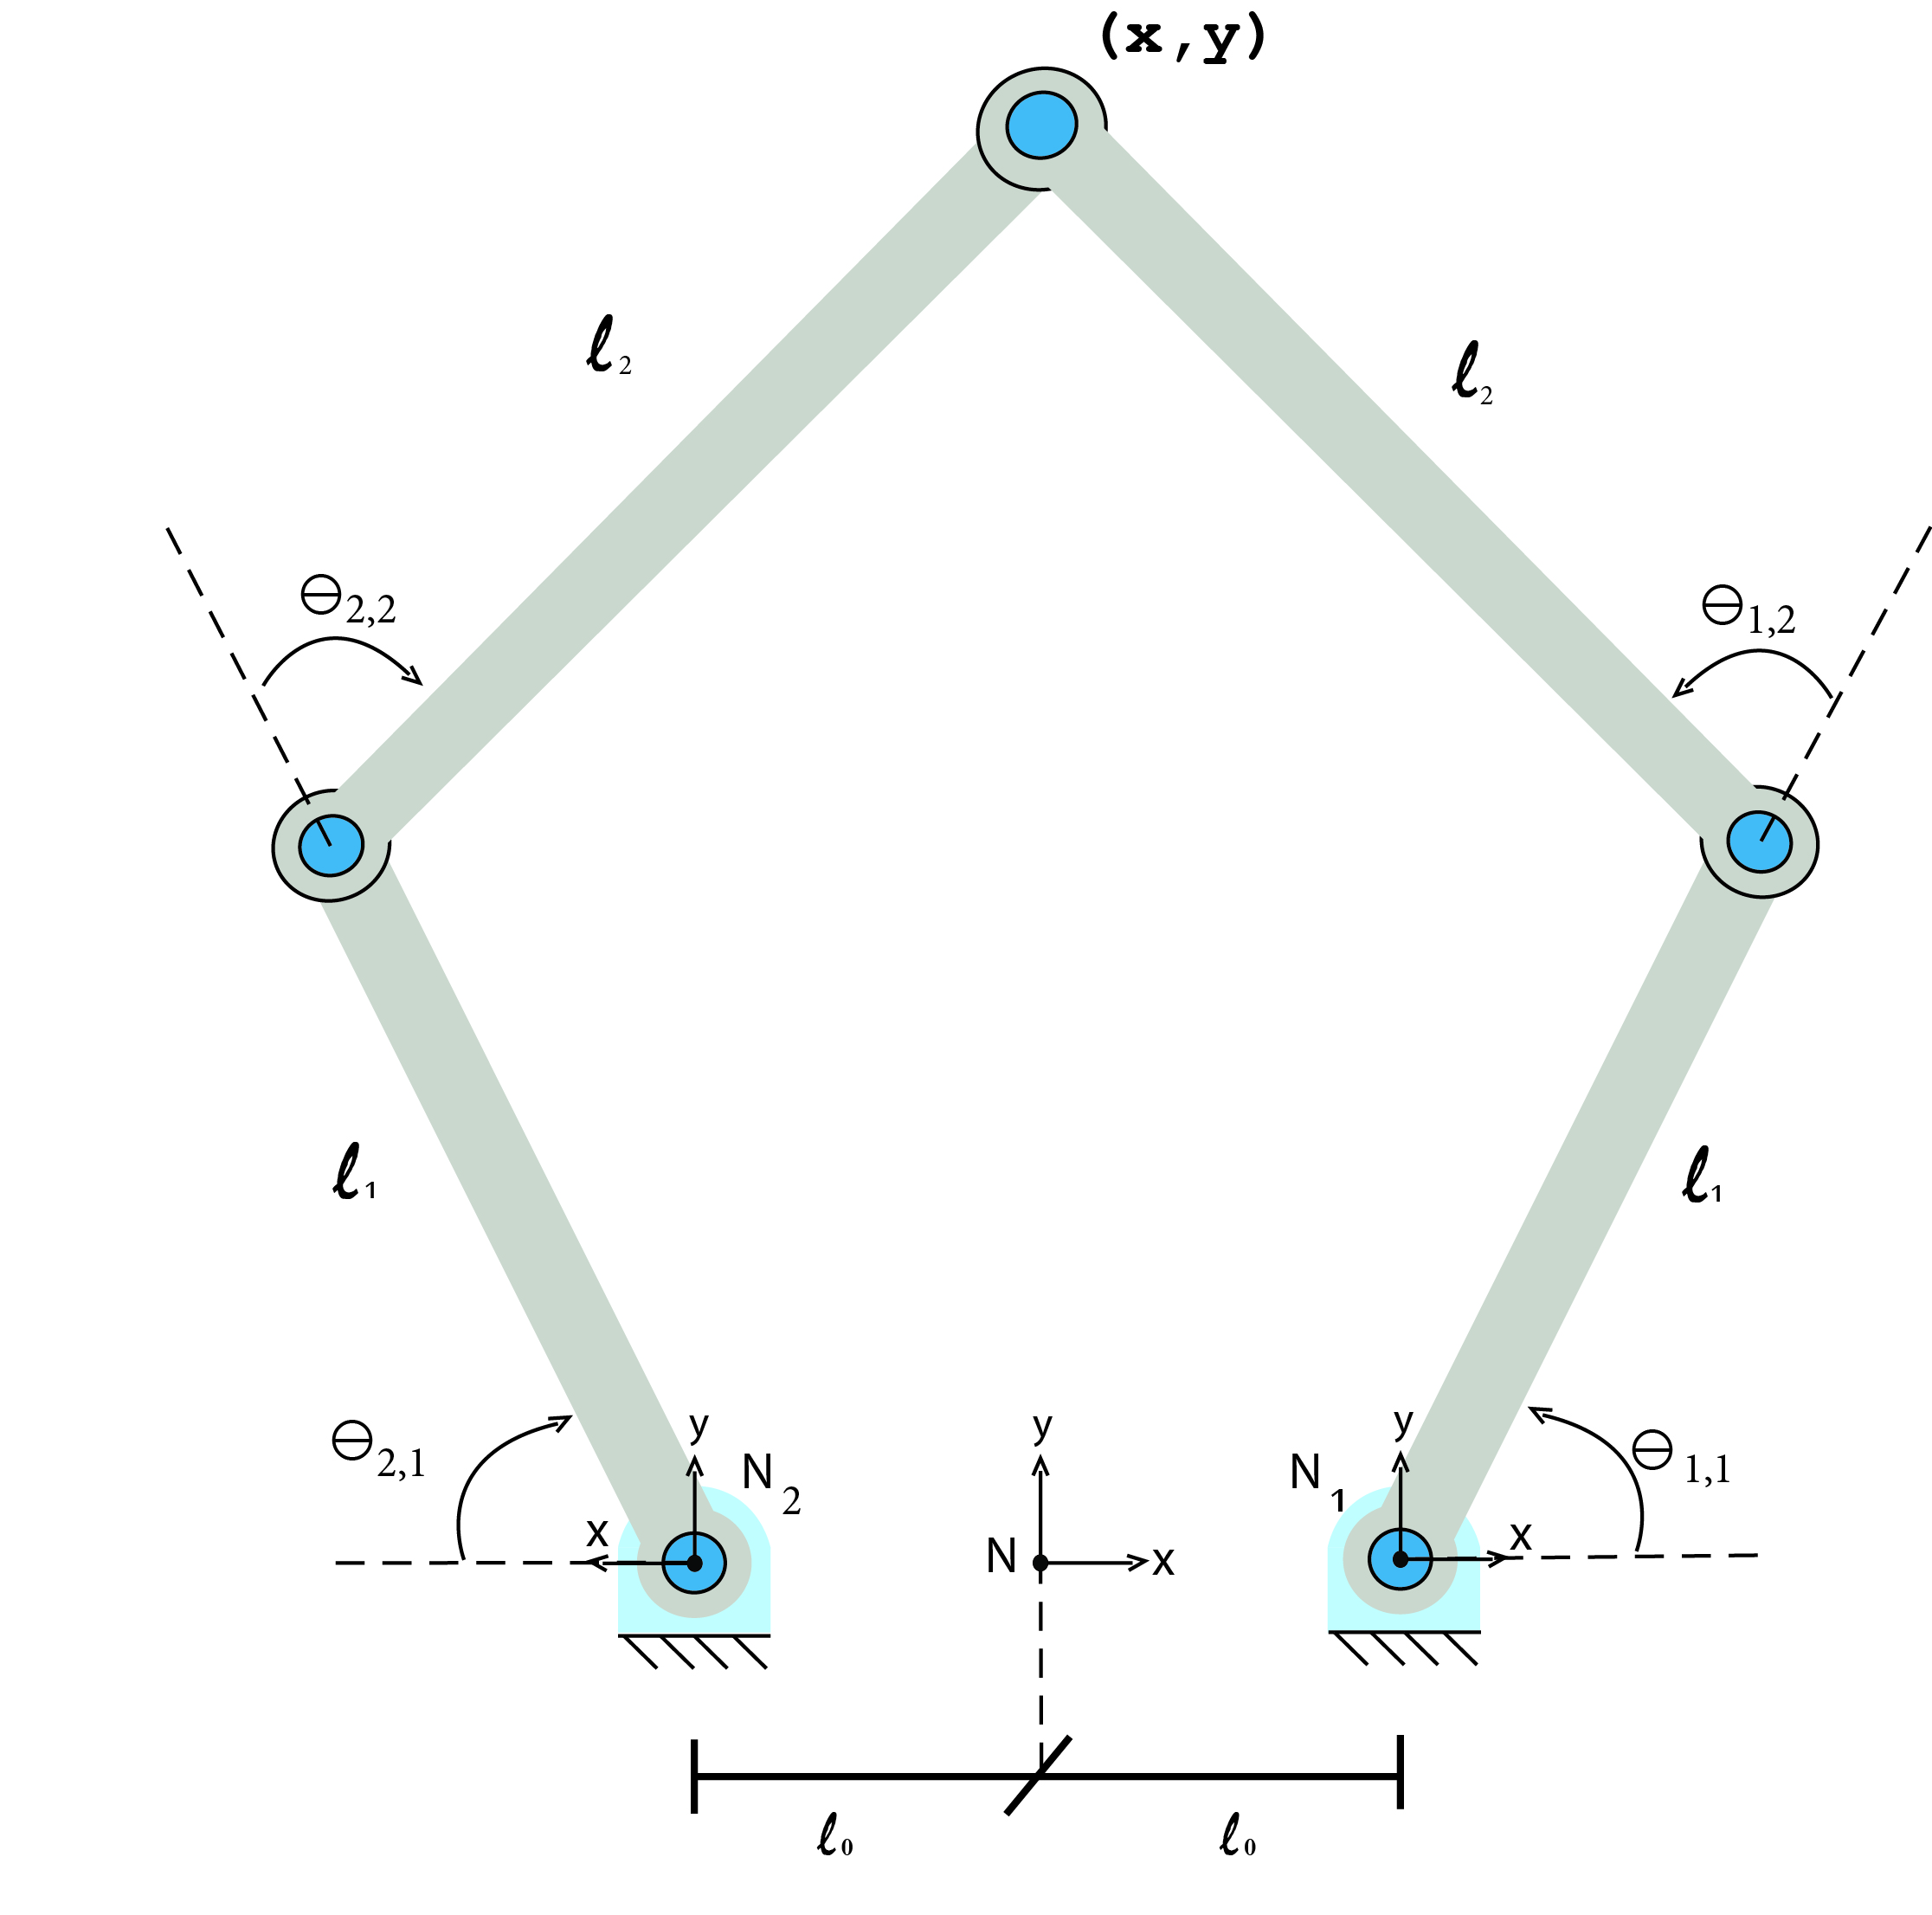
\includegraphics[scale=0.10]{../figures/5Rscan.jpg}  
	\caption{Pentágono articulado (5R)}
	\label{fig:5R}
\end{figure}

O mecanismo 5R (figura \ref{fig:5R}) será modelado através do acoplamento de 2 subsistemas seriais $\ssB_1$ e $\ssB_2$ do tipo \underline{R}\underline{R} (figura \ref{fig:RR}), e um efetuador pontual $\ssB_0$ de massa $m_0$.

\begin{figure}[h]
	\centering
	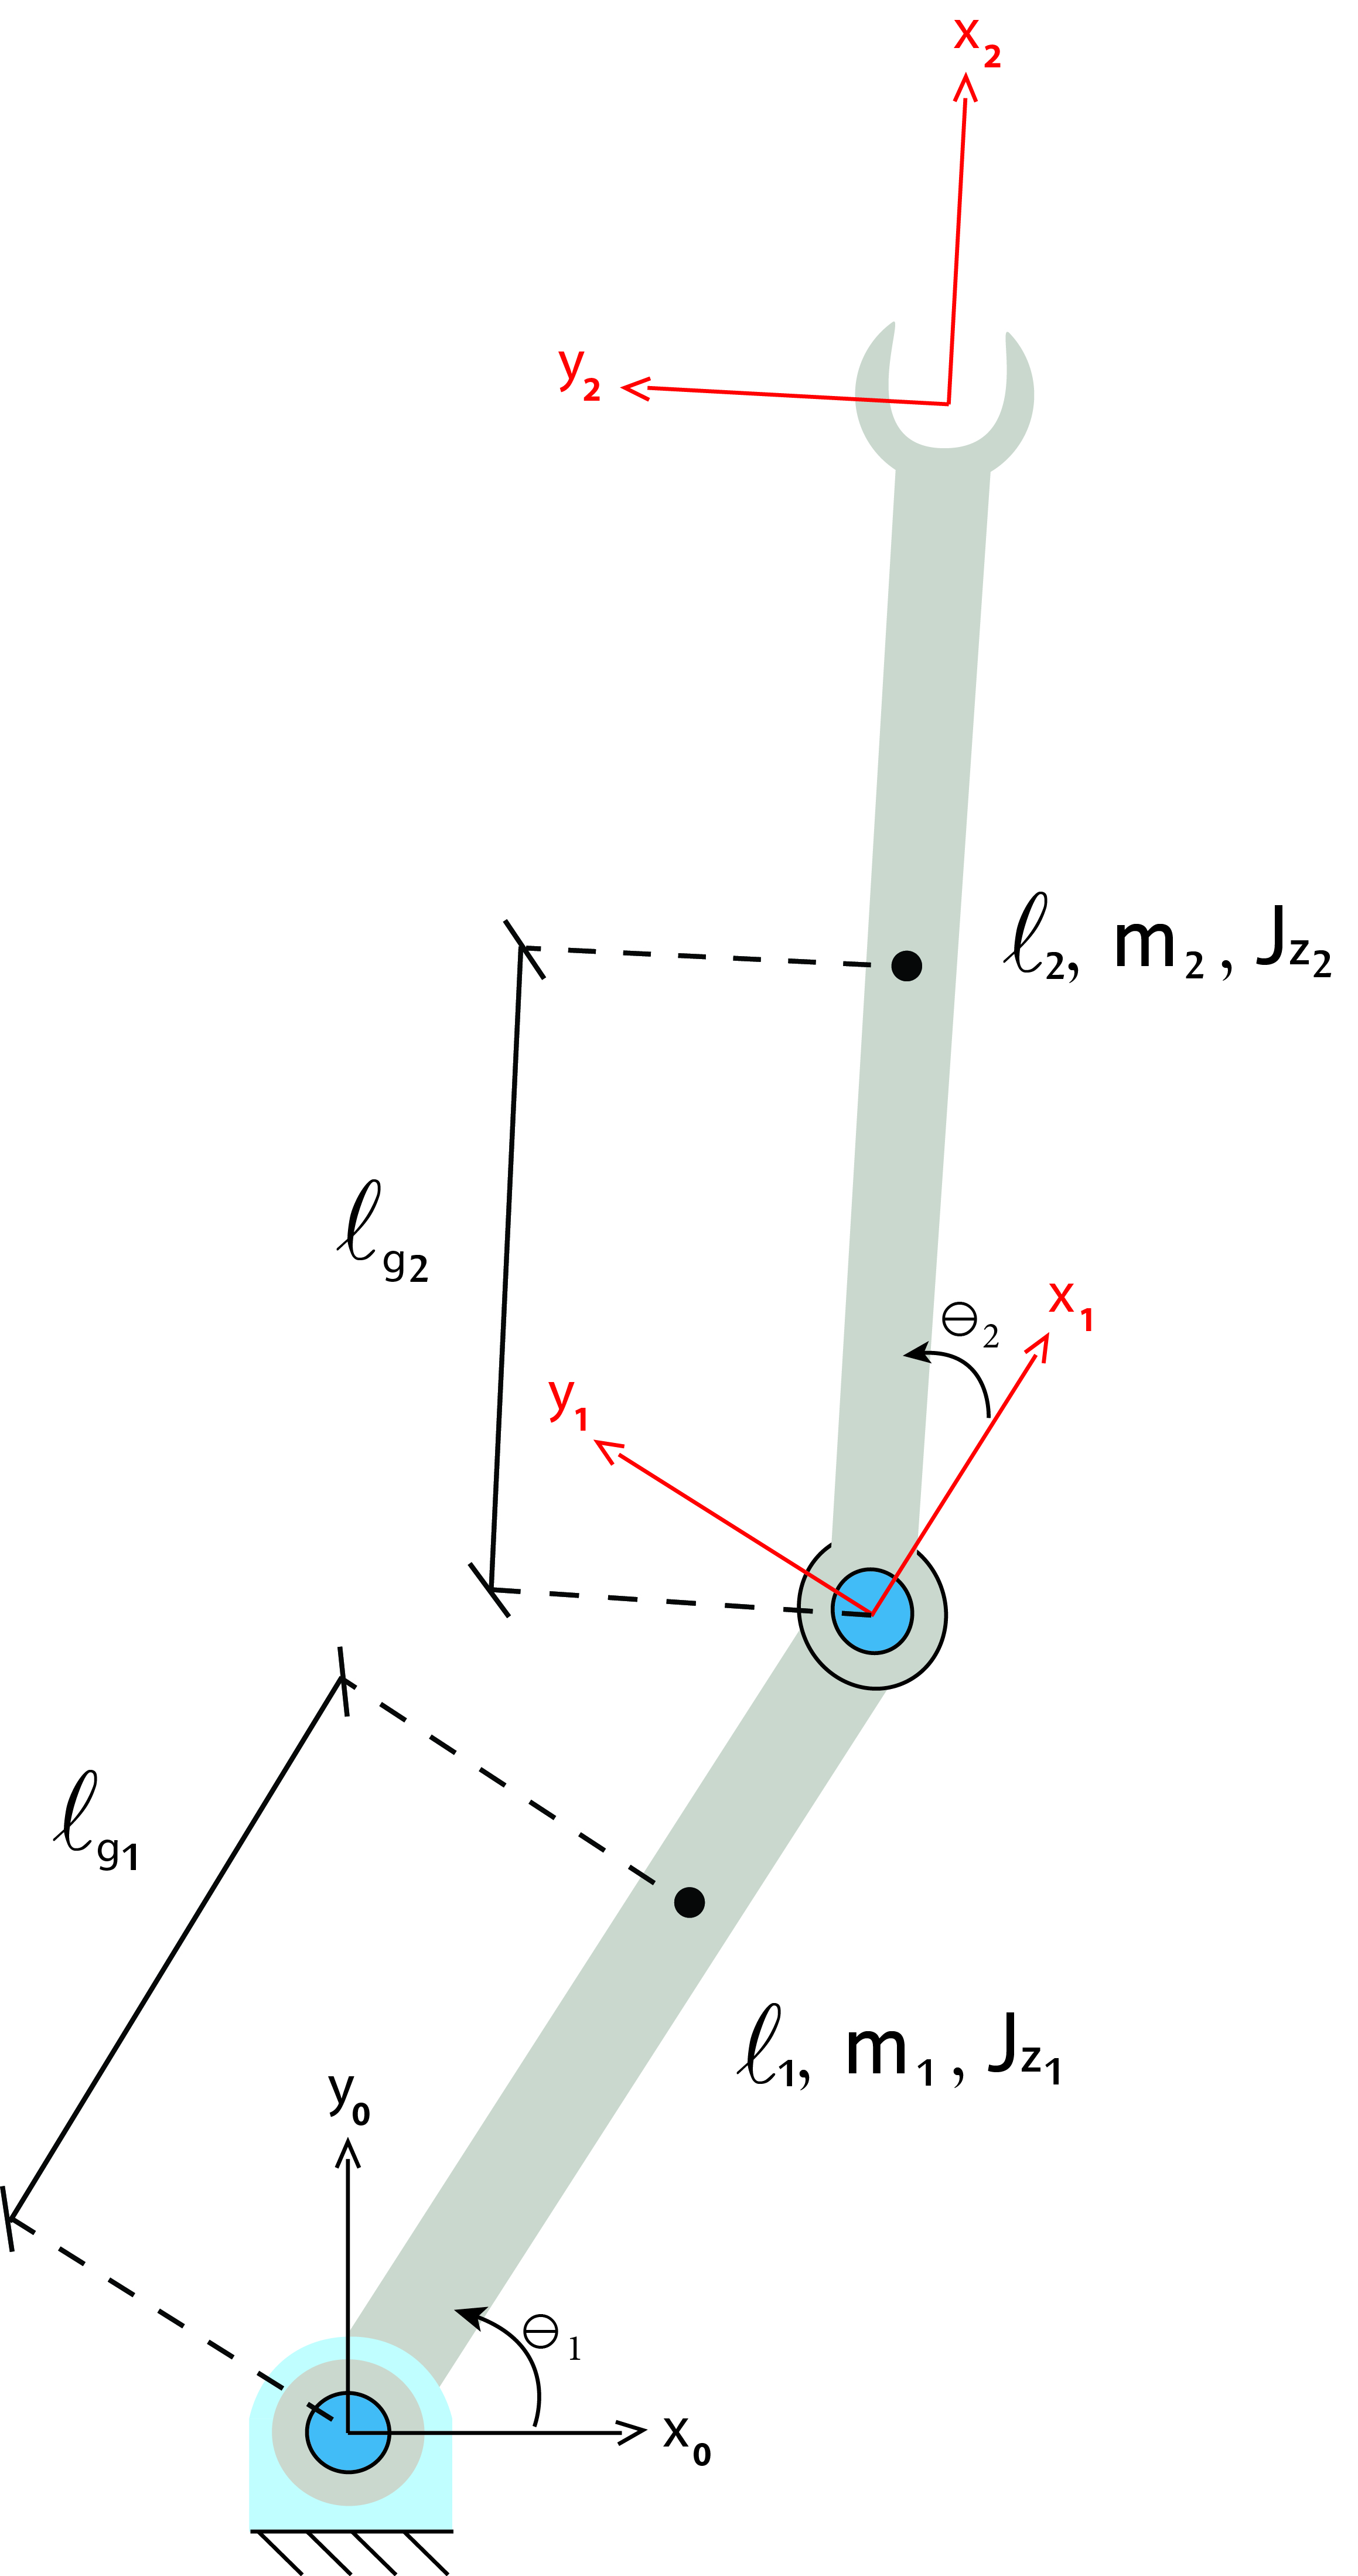
\includegraphics[scale=0.055]{../figures/RR.jpg}  
	\caption{Mecanismo \underline{R}\underline{R}}
	\label{fig:RR}
\end{figure}



\subsection{Modelo do efetuador}

De acordo com as equações \eqref{eq:Newton-EulerMat2E}, \eqref{eq:M_efetuador}, \eqref{eq:v_efetuador} e \eqref{eq:g_efetuador}, os parâmetros $m_0$ (massa do efetuador) e $\mgamma$ definem o modelo do efetuador.



%O modelo do efetuador pontual $\ssB_0$ segue o formato dado pela equação \eqref{eq:ModeloDosSubsistemas}, ou seja:
%\begin{equation}
%\overline{\mf}_{\ssB_0}(\mu_0, \mq_0, \dot{\mq}_0, \ddot{\mq}_0) =  \mu_0 - (\mM_{\ssB_0}(\mq_0) \ddot{\mq}_0 + \mv_{\ssB_0}(\mq_0,\dot{\mq}_0) + \mg_{\ssB_0}(\mq_0)) = \mzr
%\end{equation}

Para o subsistema em questão, temos:
\begin{equation}
\mq_0 = \begin{bmatrix}
x & y & z
\end{bmatrix}^\msT
\end{equation}

O vetor gravidade será considerado na direção e sentido do eixo $z$ (perpendicular ao plano), ou seja:
\begin{equation}
\mgamma = \begin{bmatrix}
0 & 0 & g
\end{bmatrix}^\msT
\end{equation}

%\begin{equation}
%\mM_{\ssB_0}(\mq_0) = \begin{bmatrix}
%m_0 & 0 \\
%0 & m_0 \\
%\end{bmatrix}
%\end{equation}
%\begin{equation}
%\mv_{\ssB_0}(\mq_0,\dot{\mq}_0) = \mzr
%\end{equation}
%\begin{equation}
%\mg_{\ssB_0}(\mq_0) = \begin{bmatrix}
%0 &
%m_0 g \\
%\end{bmatrix}^\msT
%\end{equation}
%\begin{equation}
%\mq_0 = \mq\ssh = \begin{bmatrix}
%x &
%y
%\end{bmatrix}^\msT
%\end{equation}
%\begin{equation}
%\mu_0 = \mzr
%\end{equation}



\subsection{Parâmetros de Denavit-Hartemberg das cadeias seriais}

\begin{table}[H]
\begin{center}
\caption{Parâmetros de Denavit-Hartemberg do mecanismo \underline{R}\underline{R}}
\begin{tabular}{|c|c|c|c|c|c|} 
	\hline
	\rule[-2mm]{0mm}{6mm}
	Ligamento & $a_i$ & $\alpha_i$ & $d_i$ & $\theta_i$ \\
	\hline
	\rule[-2mm]{0mm}{6mm}
	(1) & $l_1$ & $0$ & $0$ & $q_1(t)$  \\
	\rule[-1mm]{0mm}{5mm}
	(2) & $l_2$ & $0$ & $0$ & $q_2(t)$  \\
	\hline
\end{tabular}
\label{tab:DH}
\end{center}
\end{table}

\subsection{Arquitetura do mecanismo paralelo}

É possível relacionar as coordenadas um ponto no espaço descrito no sistema $\ttN_0$ com as coordenadas do mesmo ponto escritas nos sistemas $\ttN_1$ e $\ttN_2$ da seguinte maneira:
\begin{equation}
\vct{\ttp}_{\ttN_0} = \begin{bmatrix}
1 & 0 & 0 \\
0 & 1 & 0 \\
0 & 0 & 1 \\
\end{bmatrix}
\cdot
\vct{\ttp}_{\ttN_1}
+
\begin{bmatrix}
l_0 \\
0 \\
0 
\end{bmatrix}
\end{equation}
\begin{equation}
\vct{\ttp}_{\ttN_0} = \begin{bmatrix}
-1 & 0 & 0 \\
0 & 1 & 0 \\
0 & 0 & -1 \\
\end{bmatrix}
\cdot
\vct{\ttp}_{\ttN_2}
+
\begin{bmatrix}
-l_0 \\
0 \\
0 
\end{bmatrix}
\end{equation}

Escolhendo o ponto $\ttp$ como sendo o efetuador do mecanismo paralelo, o qual tem a mesma localização dos efetuadores das cadeias serias neste caso, temos:
\begin{equation}
\mq_0 = 
\begin{bmatrix}
1 & 0 & 0 \\
0 & 1 & 0 \\
0 & 0 & 1 \\
\end{bmatrix}
\cdot
\mx_1(\mq_1)
+
\begin{bmatrix}
l_0 \\
0 \\
0 \\
\end{bmatrix}
\end{equation}
\begin{equation}
\mq_0 = 
\begin{bmatrix}
-1 & 0 & 0 \\
0 & 1 & 0 \\
0 & 0 & -1 \\
\end{bmatrix}
\cdot
\mx_2(\mq_2)
+
\begin{bmatrix}
-l_0 \\
0 \\
0 \\
\end{bmatrix}
\end{equation}

Sendo assim, temos que os vínculos de posição são dados por:
\begin{equation}
\overline{\mq}(\mq) =
\begin{bmatrix}
1 & 0 & 0 \\
0 & 1 & 0 \\
0 & 0 & 1 \\
1 & 0 & 0 \\
0 & 1 & 0 \\
0 & 0 & 1 \\
\end{bmatrix}
\cdot
\mq_0
-
\begin{bmatrix}
1 & 0 & 0 & 0 & 0 & 0 \\
0 & 1 & 0 & 0 & 0 & 0 \\
0 & 0 & 1 & 0 & 0 & 0 \\
0 & 0 & 0 & -1 & 0 & 0 \\
0 & 0 & 0 & 0 & 1 & 0 \\
0 & 0 & 0 & 0 & 0 & -1 \\
\end{bmatrix}
\cdot
\mx(\mq_\emptyset)
-
\begin{bmatrix}
l_0 \\
0 \\
0 \\
-l_0 \\
0 \\
0 \\
\end{bmatrix}
= \mzr
\end{equation}

Sendo assim, as matrizes que descrevem a arquitetura do mecanismo são dadas por:
\begin{equation}
\md = \begin{bmatrix}
l_0 &
0 &
0 &
-l_0 &
0 &
0 
\end{bmatrix}^\msT
\end{equation}
\begin{equation}
\mD = \begin{bmatrix}
1 & 0 & 0 & 1 & 0 & 0 \\
0 & 1 & 0 & 0 & 1 & 0 \\
0 & 0 & 1 & 0 & 0 & 1 \\
\end{bmatrix}^\msT
\end{equation}
\begin{equation}
\mE = \begin{bmatrix}
1 & 0 & 0 & 0 & 0 & 0 \\
0 & 1 & 0 & 0 & 0 & 0 \\
0 & 0 & 1 & 0 & 0 & 0 \\
0 & 0 & 0 & -1 & 0 & 0 \\
0 & 0 & 0 & 0 & 1 & 0 \\
0 & 0 & 0 & 0 & 0 & -1 \\
\end{bmatrix}
\end{equation}
\begin{equation}
\mF = \mzr
\end{equation}
%\begin{equation}
%\mP = \mQ = \mR = \vct{\varnothing}
%\end{equation}

\subsection{Coordenadas dependentes e independentes}

Tende em vista que o mecanismo em questão possui duas cadeias seriais de 2 graus de liberdade, temos:
\begin{equation}
\mq = \begin{bmatrix}
\mq_0 \\
\mq_1 \\
\mq_2
\end{bmatrix} =
\begin{bmatrix}
x \\
y \\
z \\
\theta_{1,1} \\
\theta_{1,2} \\
\theta_{2,1} \\
\theta_{2,2} \\
\end{bmatrix}
\end{equation}

Neste caso escolheremos as coordenadas $x$ e $y$ para serem as coordenadas generalizadas independentes (tendo em vista que o mecanismo possui dois graus de liberdade, ou seja:
\begin{equation}
\mq\ssh = \begin{bmatrix}
x & y
\end{bmatrix}^\msT
\end{equation}
\begin{equation}
\mq\cir = \begin{bmatrix}
z & \theta_{1,1} & \theta_{1,2} & \theta_{2,1} & \theta_{2,2}
\end{bmatrix}^\msT
\end{equation}

Sendo assim, temos que as matrizes $\mQ\ssh$ e $\mQ\cir$ são dadas por:
\begin{multicols}{2}
\begin{equation}
\mQ\ssh = \begin{bmatrix}
1 & 0 \\
0 & 1 \\
0 & 0 \\
0 & 0 \\
0 & 0 \\
0 & 0 \\
0 & 0 \\
\end{bmatrix}
\end{equation} \\
\begin{equation}
\mQ\cir = \begin{bmatrix}
0 & 0 & 0 & 0 & 0 \\
0 & 0 & 0 & 0 & 0 \\
1 & 0 & 0 & 0 & 0 \\
0 & 1 & 0 & 0 & 0 \\
0 & 0 & 1 & 0 & 0 \\
0 & 0 & 0 & 1 & 0 \\
0 & 0 & 0 & 0 & 1 \\
\end{bmatrix}
\end{equation}
\end{multicols}

\subsection{Simulação dinâmica direta}

Para realizar a simulação dinâmica direta, definimos:

\subsubsection{Parâmetros do modelo}

Definimos os seguinte parâmetros para o modelo o mecanismo em questão na tabela \ref{tab:parametrosSimulacao}:

\begin{table}[H] 
\centering
\caption{Parâmetros do mecanismo}
\label{tab:parametrosSimulacao}
\begin{tabular}{l|l|l}
Parâmetros   & Valores                  & Unidades      \\ \hline
$l_0$        & $0.050$                     & $m$        \\
$l_1$        & $0.120$                     & $m$        \\
$l_2$        & $0.150$                     & $m$        \\
$l_{g1}$     & $0.060$                     & $m$        \\
$l_{g2}$     & $0.075$                    & $m$        \\
$m_0$        & $0.000$                    & $kg$       \\
$m_1$        & $0.143$                    & $kg$       \\
$m_2$        & $0.171$                    & $kg$       \\
$J_{z1}$     & $1.716 \cdot 10^{-4}$    & $kg.m^{2}$ \\
$J_{z2}$     & $3.206 \cdot 10^{-4}$    & $kg.m^{2}$ \\
\end{tabular}
\end{table}

\subsubsection{Espaço de trabalho}

Dados os parâmetros geométricos definidos na tabela \ref{tab:parametrosSimulacao}, obtemos o seguinte espaço de trabalho para o mecanismo (figura \ref{fig:RRWS}):

\begin{figure}[h]
	\centering
	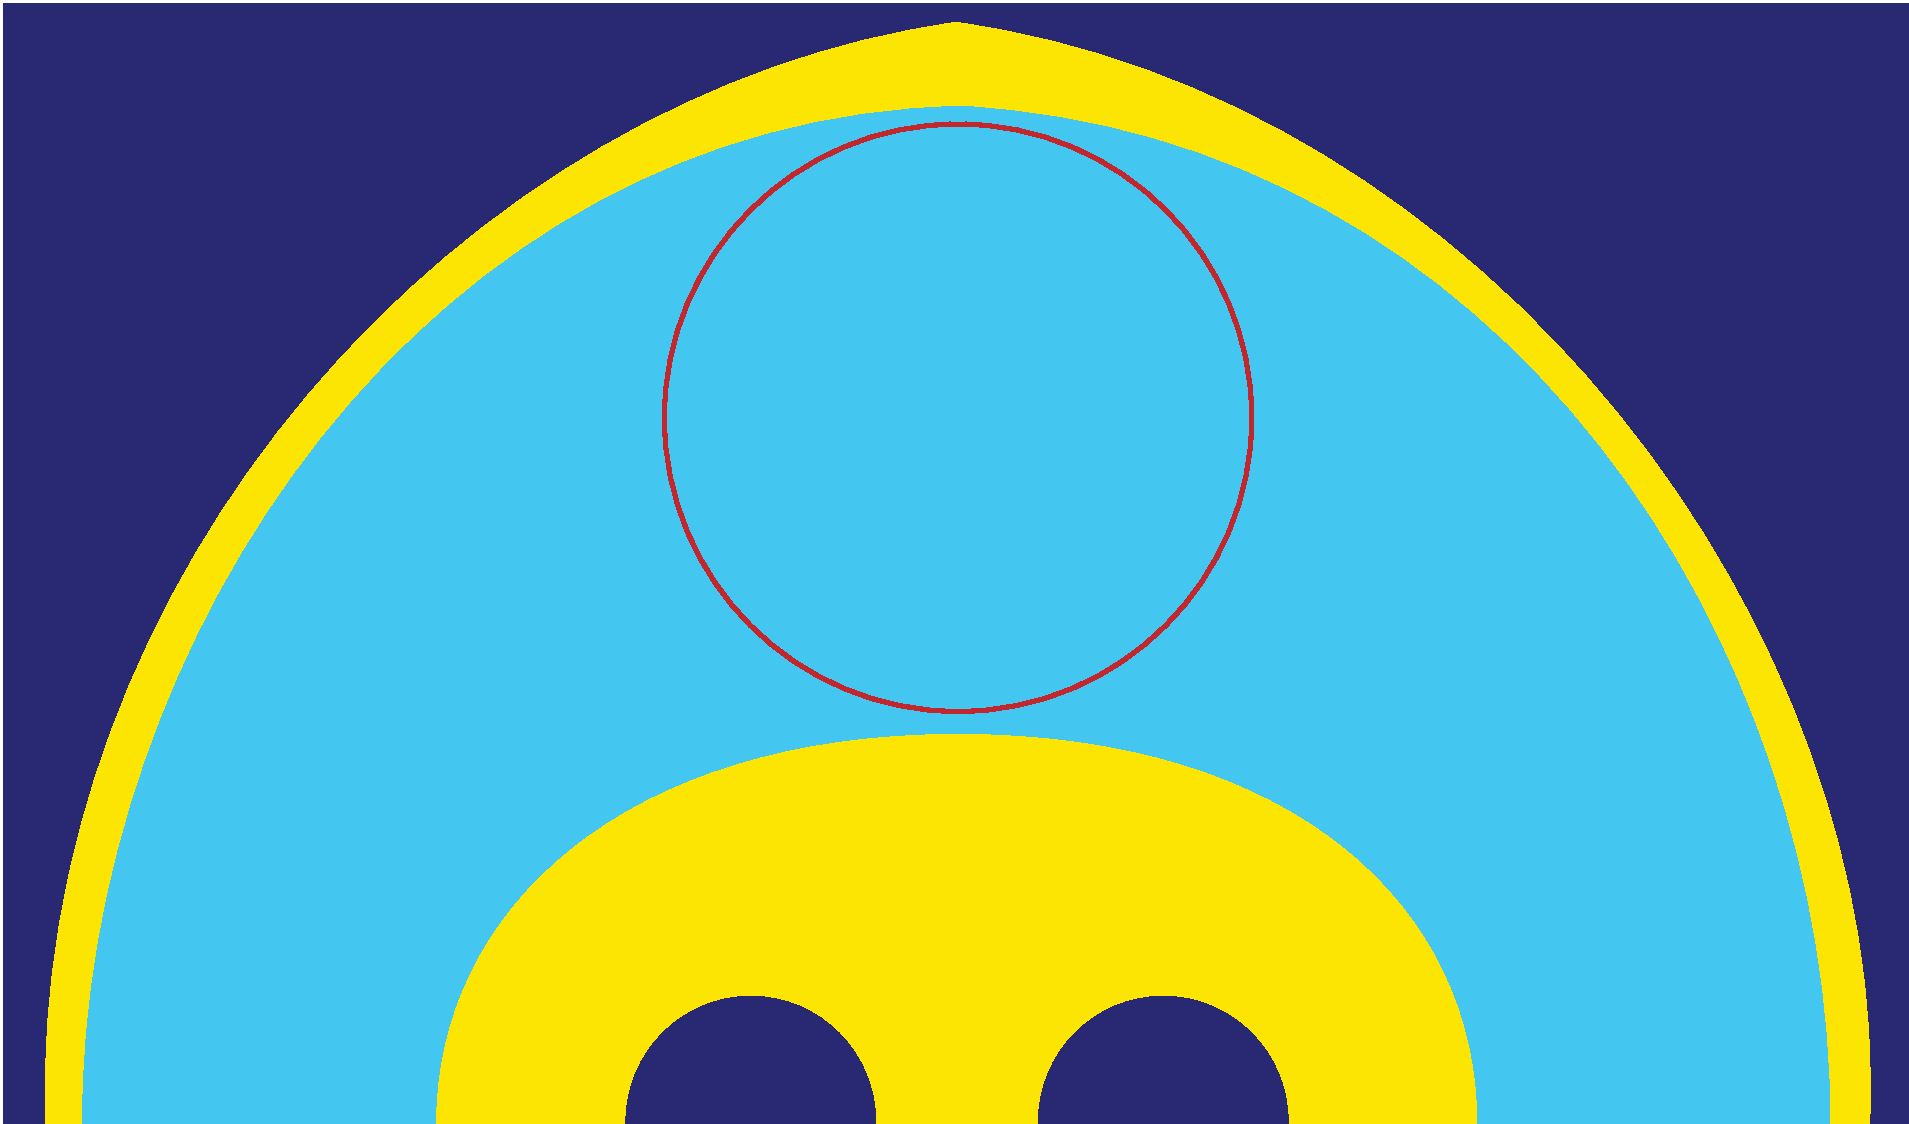
\includegraphics[scale=0.25]{../figures/Workspace.pdf}  
	\caption{Espaço de trabalho do mecanismo 5R}
	\label{fig:RRWS}
\end{figure}

A região em azul escuro é a região não pertencente ao espaço de trabalho do mecanismo. As regiões em azul claro, em amarelo, e em vermelho são regiões pertencententes ao espaço de trabalho do mecanismo. A região a amarela é considerada singular (próxima a singularidades) e a vermelha é a trajetória a ser seguida pelo mecanismo.

\subsubsection{Condições iniciais}
\begin{equation}
\begin{cases}
x(0) = 0.07 m\\
y(0) = 0.17 m \\
\dot{x}(0) = 0 \\
\dot{y}(0) = 0 \\
\end{cases}
\end{equation}

\subsubsection{Trajetória de referência}
\begin{equation}
\begin{cases}
x_{d}(t) = 0.07 \cos(2 \pi t) \\
y_{d}(t) = 0.17 + 0.07 \sin(2 \pi t) \\
\end{cases}
\end{equation}

\subsubsection{Parâmetros do controlador}
$$ \underline{k}_p = \lambda^2 \mone $$
$$ \underline{k}_v = 2\lambda \mone $$
$$ \lambda = 40 \, rad/s $$

Os parâmetros do Controle por Torque Computado foram escolhidos de modo que a dinâmica do erro de controle se comporte como uma dinâmica de segunda ordem com amortecimento crítico. O valor de $\lambda$ foi escolhido para o tempo de assentamento do erro de controle seja de $0.1s$, o que é razoável para um sistema mecânico.

\subsubsection{Simulações}

Nas figuras \ref{fig:Torque1_0} a \ref{fig:ey_40} são apresentados os resultados de 3 simulações dinâmicas diretas do mecanismo 5R, considerando 3 níveis de incerteza do modelo: 0\%, 20\% e 40\%. Todas as simulações são realizadas utilizando a lei de Control por Torque Computado apresentada na seção \ref{sec:CTC}, utilizando os parâmetros definidos na tabela \ref{tab:parametrosSimulacao}.

\begin{multicols}{2}
\begin{figure}[H]
	\centering
	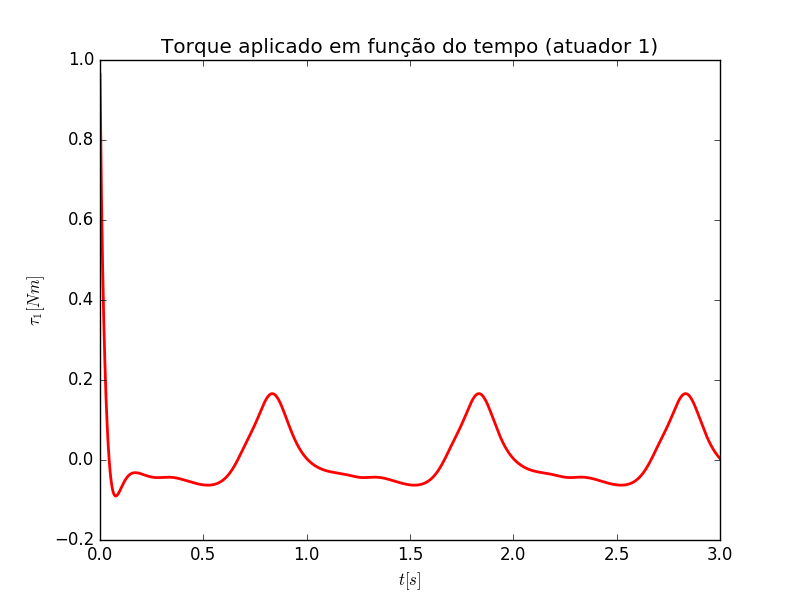
\includegraphics[scale=0.42]{imagens/tau1_0.png}  
	\caption{$\tau_1$: sem incerteza}
	\label{fig:Torque1_0}
\end{figure}
\begin{figure}[H]
	\centering
	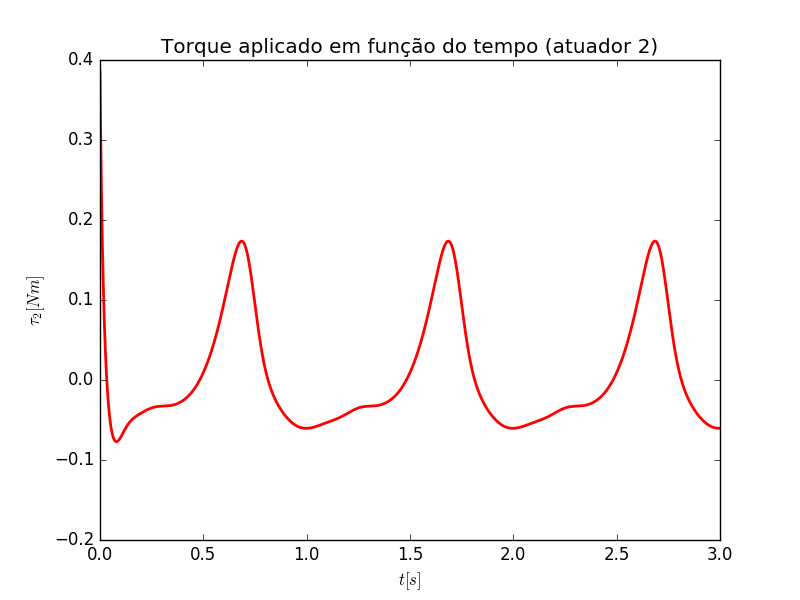
\includegraphics[scale=0.42]{imagens/tau2_0.png}  
	\caption{$\tau_2$: sem incerteza}
	\label{fig:Torque2_0}
\end{figure}
\end{multicols}

\begin{multicols}{2}
\begin{figure}[H]
	\centering
	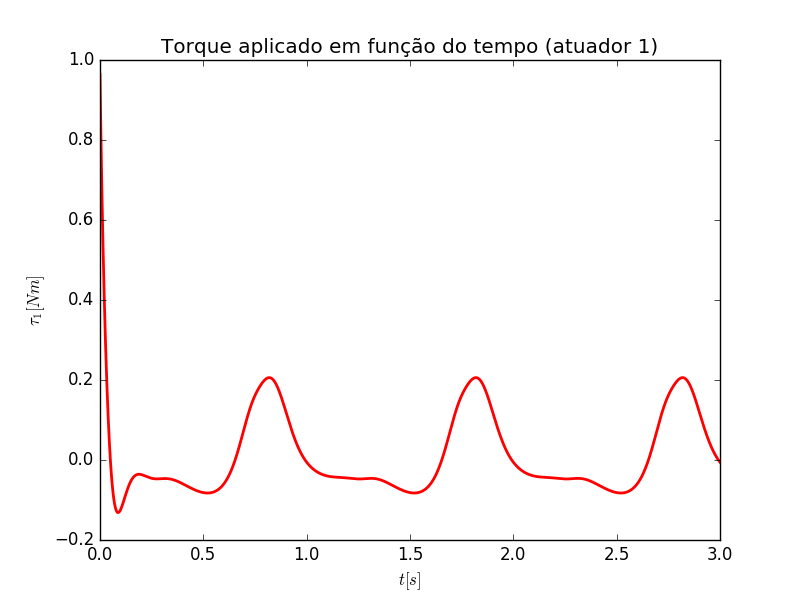
\includegraphics[scale=0.42]{imagens/tau1_20.png}  
	\caption{$\tau_1$: 20\% de incerteza}
	\label{fig:Torque1_20}
\end{figure}
\begin{figure}[H]
	\centering
	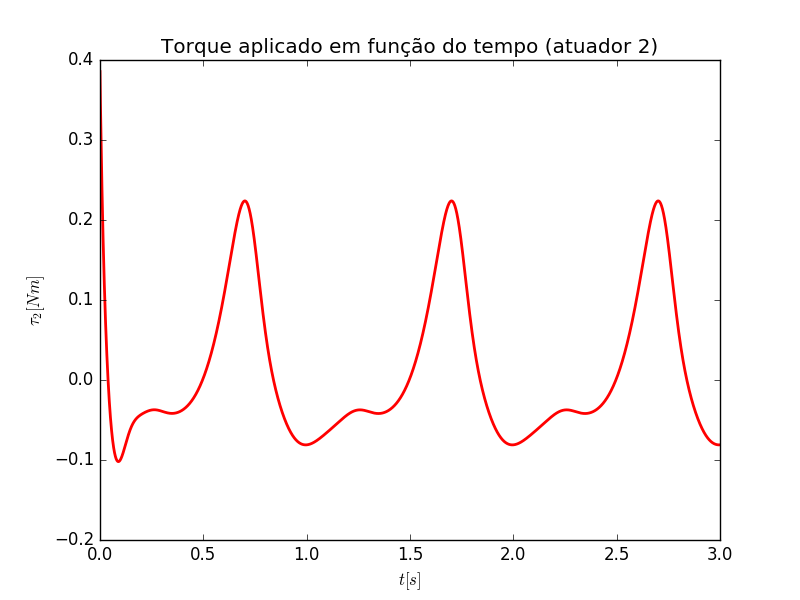
\includegraphics[scale=0.42]{imagens/tau2_20.png}  
	\caption{$\tau_2$: 20\% de incerteza}
	\label{fig:Torque2_20}
\end{figure}
\end{multicols}

\begin{multicols}{2}
\begin{figure}[H]
	\centering
	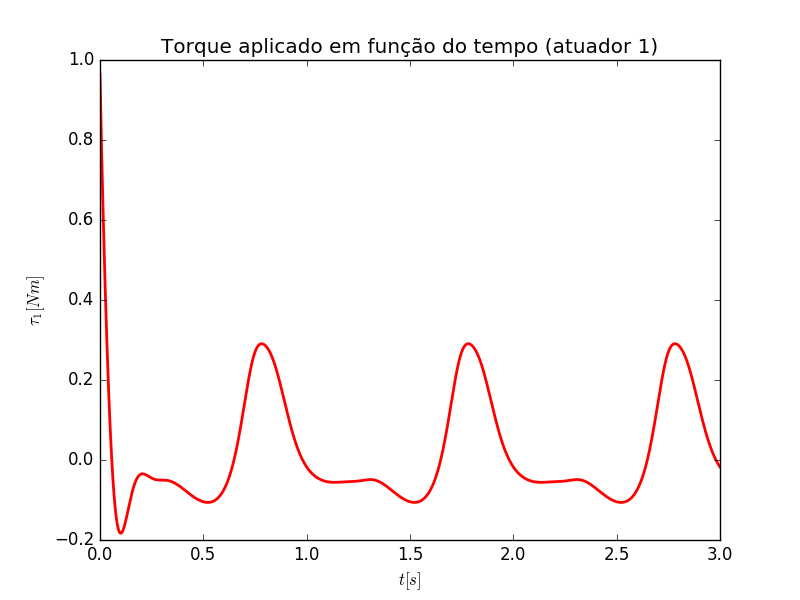
\includegraphics[scale=0.42]{imagens/tau1_40.png}  
	\caption{$\tau_1$: 40\% de incerteza}
	\label{fig:Torque1_40}
\end{figure}
\begin{figure}[H]
	\centering
	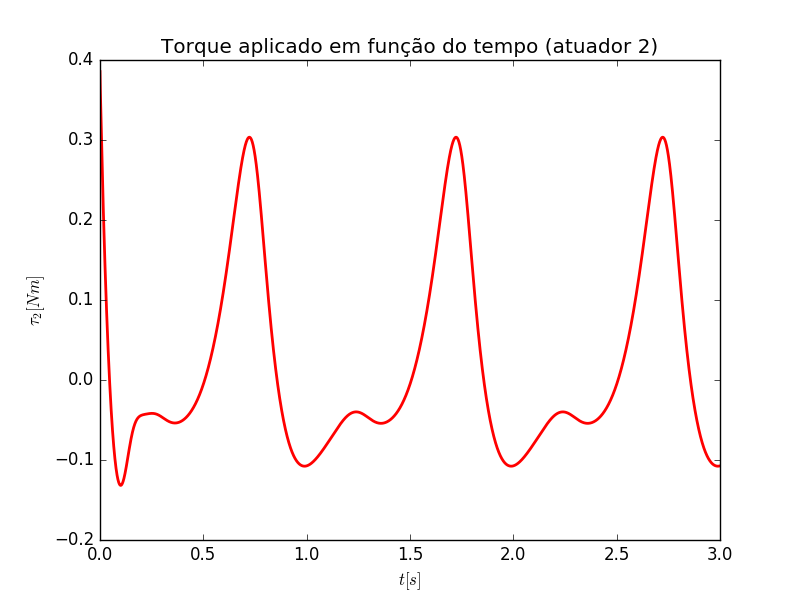
\includegraphics[scale=0.42]{imagens/tau2_40.png}  
	\caption{$\tau_2$: 40\% de incerteza}
	\label{fig:Torque2_40}
\end{figure}
\end{multicols}  

\newpage

\begin{multicols}{2}
\begin{figure}[H]
	\centering
	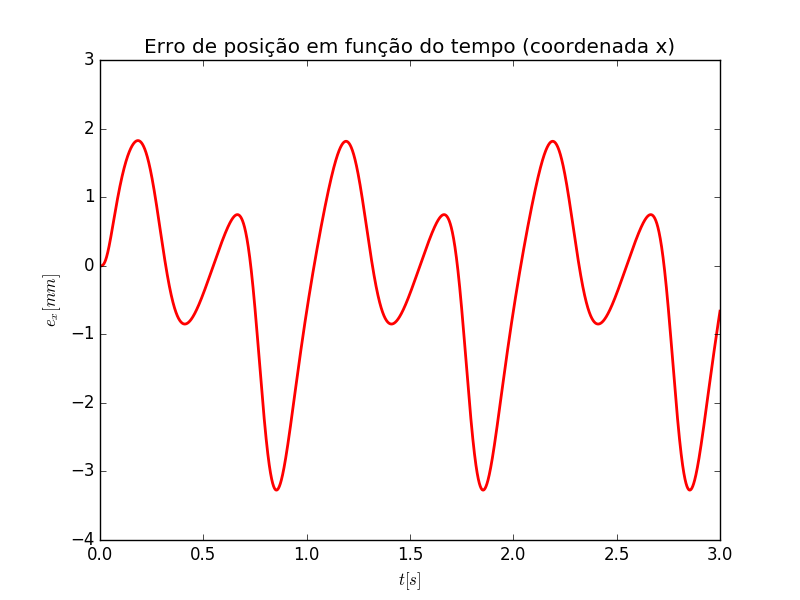
\includegraphics[scale=0.42]{imagens/ex_0.png}  
	\caption{$e_x$: sem incerteza}
	\label{fig:ex_0}
\end{figure}
\begin{figure}[H]
	\centering
	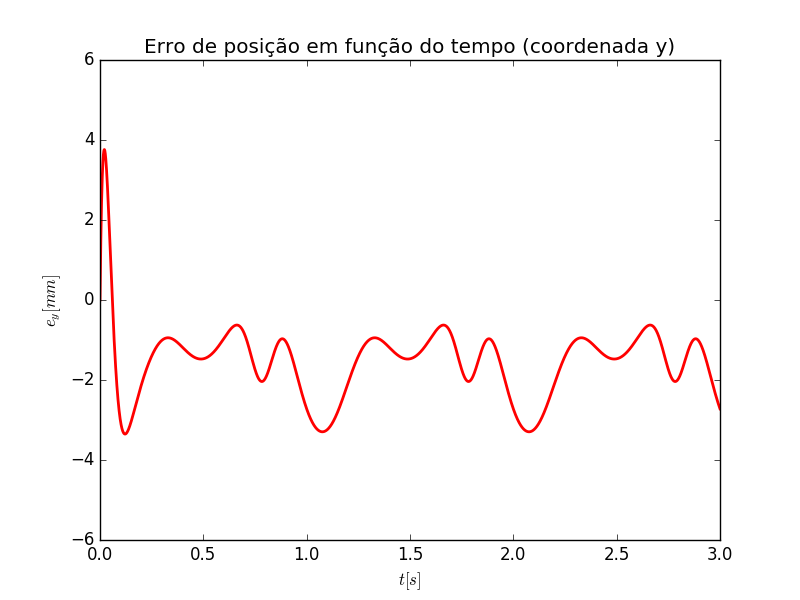
\includegraphics[scale=0.42]{imagens/ey_0.png}  
	\caption{$e_y$: sem incerteza}
	\label{fig:ey_0}
\end{figure}
\end{multicols}

\begin{multicols}{2}
\begin{figure}[H]
	\centering
	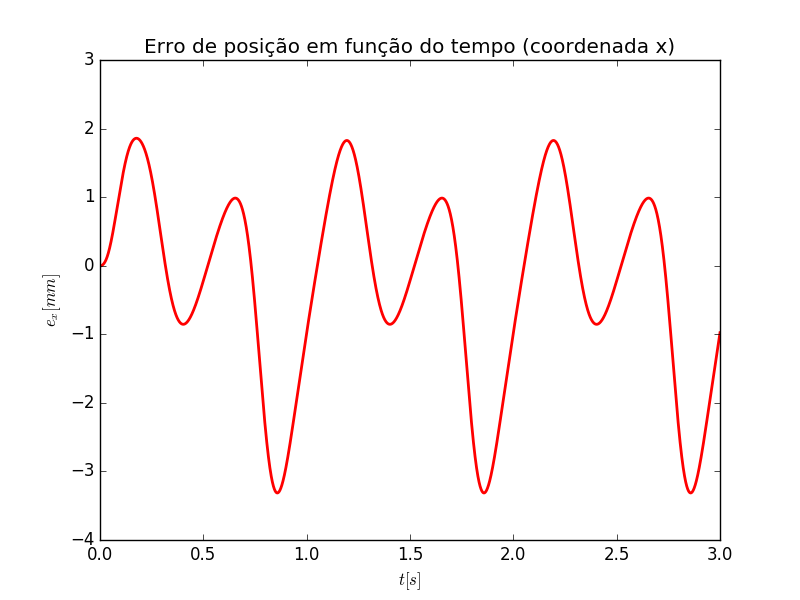
\includegraphics[scale=0.42]{imagens/ex_20.png}  
	\caption{$e_x$: 20\% de incerteza}
	\label{fig:ex_20}
\end{figure}
\begin{figure}[H]
	\centering
	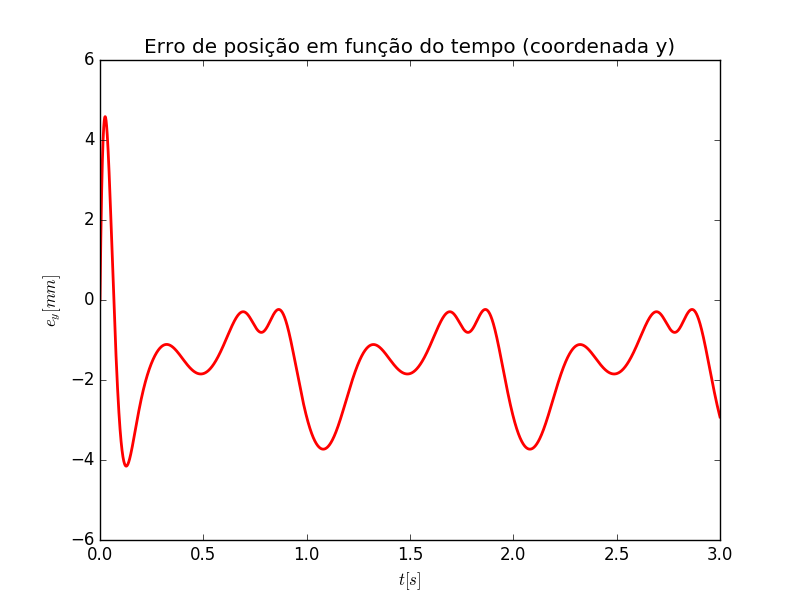
\includegraphics[scale=0.42]{imagens/ey_20.png}  
	\caption{$e_y$: 20\% de incerteza}
	\label{fig:ey_20}
\end{figure}
\end{multicols}

\begin{multicols}{2}
\begin{figure}[H]
	\centering
	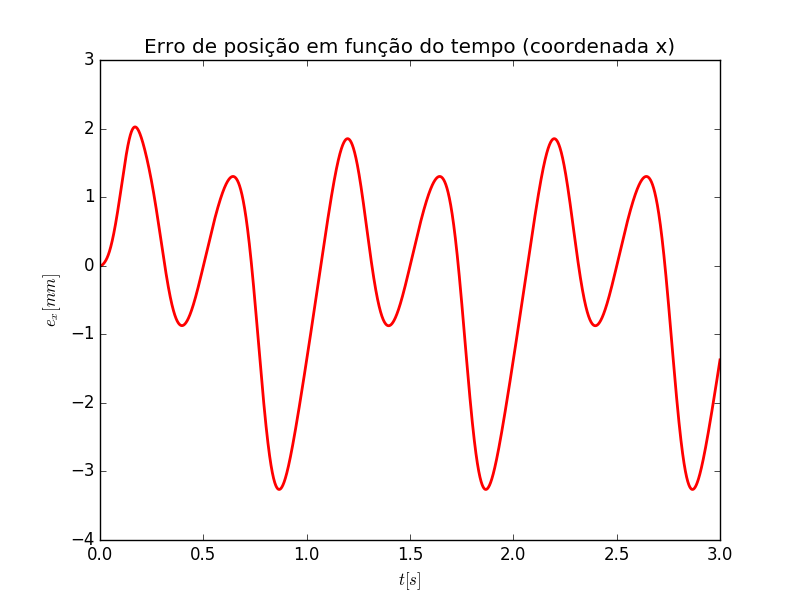
\includegraphics[scale=0.42]{imagens/ex_40.png}  
	\caption{$e_x$: 40\% de incerteza}
	\label{fig:ex_40}
\end{figure}
\begin{figure}[H]
	\centering
	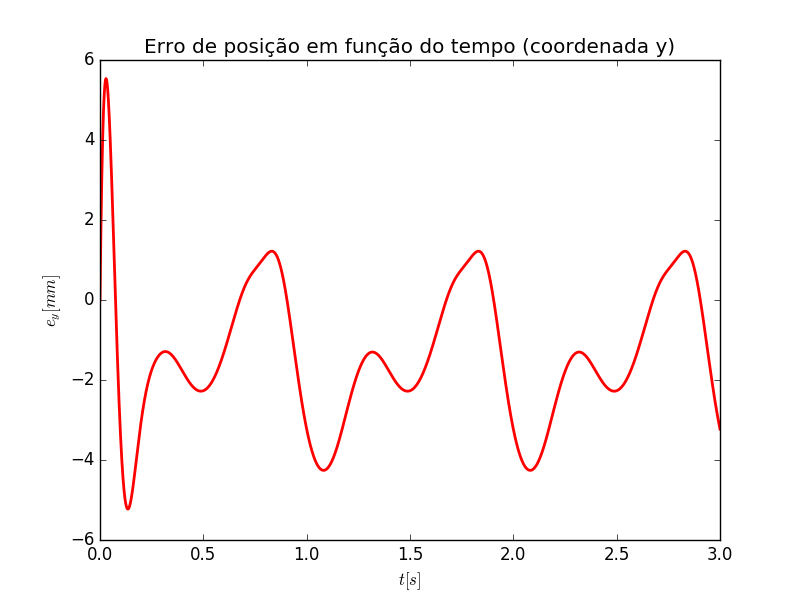
\includegraphics[scale=0.42]{imagens/ey_40.png}  
	\caption{$e_y$: 40\% de incerteza}
	\label{fig:ey_40}
\end{figure}
\end{multicols}

Nos gráficos pode-se claramente observar o aumento do esforço de controle conforme o nível de incerteza cresce. Também é possível observar que o perfil do erro na coordenada $x$ não sofreu muita influência com o aumento do nível de incerteza, enquando o perfil do erro em $y$ muda bastante de formato.

Tendo em vista que o presente trabalho tem caráter experimental, as comparações entre o desempenho de diferentes estratégias de controle serão feitas baseadas nos resultados obtidos experimentalmente.

\section{Ensaios Experimentais}

Nesta sessão, será descrita a bancada experimental e serão apresentados e discutidos os resultados experimentais do controle do mecanismo 5R utilizando 8 diferentes estratégias de controle.

\subsection{Bancada experimental}

A bancada é constituída de:

\begin{itemize}
\item 2 motores DC modelo PM70 da AMETEK com as seguintes características:
\begin{itemize}
\item Corrente nominal de $13A$ 
\item Torque nominal de $0.5Nm$
\item Potência nominal de $250W$
\item Tensão de alimentação de $24V$
\item Rotação nominal de $3600 rpm$
\item Peso de $1.80 kgf$ 
\end{itemize}
\item  2 enconders incrementais do modelo E40S com as seguintes características:
\begin{itemize}
\item Resolução de $5000 pulsos/volta$.
\item Tensão de alimentação de $12V$ a $24V$
\item 3 canais de saída A, B e Z
\end{itemize}
\item 1 driver modelo Pololu Dual VNH5019 Motor Driver Shield com as seguintes características.
\begin{itemize}
\item Tensão de operação: de $5.5V$ a $24V$
\item Corrente de saída: até $12A$ contínuos (30A de pico)
\item Dois canais de saída para motor
\item Entrada de tensão compatível com os padrões $5V$ e $3.3V$
\item Frequência de operação do PWM de até $20kHz$
\end{itemize}
\item 1 Microprocessador responsável pela execução das malhas de controle. O modelo utilizado foi o \textit{Raspberry Pi 2 Model B} com as seguintes características:
\begin{itemize}
\item Processador: quadcore ARMv7
\item 1GB RAM
\item Alimentação de $5V$, $2A$
\end{itemize}
\item 1 Fonte de tensão chaveada com as seguintes características:
\begin{itemize}
\item Tensão nominal de $24V$
\item Corrente saída de até $16.25A$
\end{itemize}
\item 1 Placa de conversão de níveis de tensão de fabricação própria com as seguintes características:
\begin{itemize}
\item Converte os $24V$ gerados pela fonte chaveada para $15V$, para alimentar os encoders
\item Converte os níveis de tensão das saídas dos encoders de $0V-15V$ para $0V-3.3V$, para poder mandar os sinais do encoder para o \textit{Raspberry Pi}
\end{itemize}
\end{itemize}

Boa parte dos elementos da bancada podem ser vistos na figura \ref{fig:BancadaClara1}.

\begin{figure}[H]
    \centering
    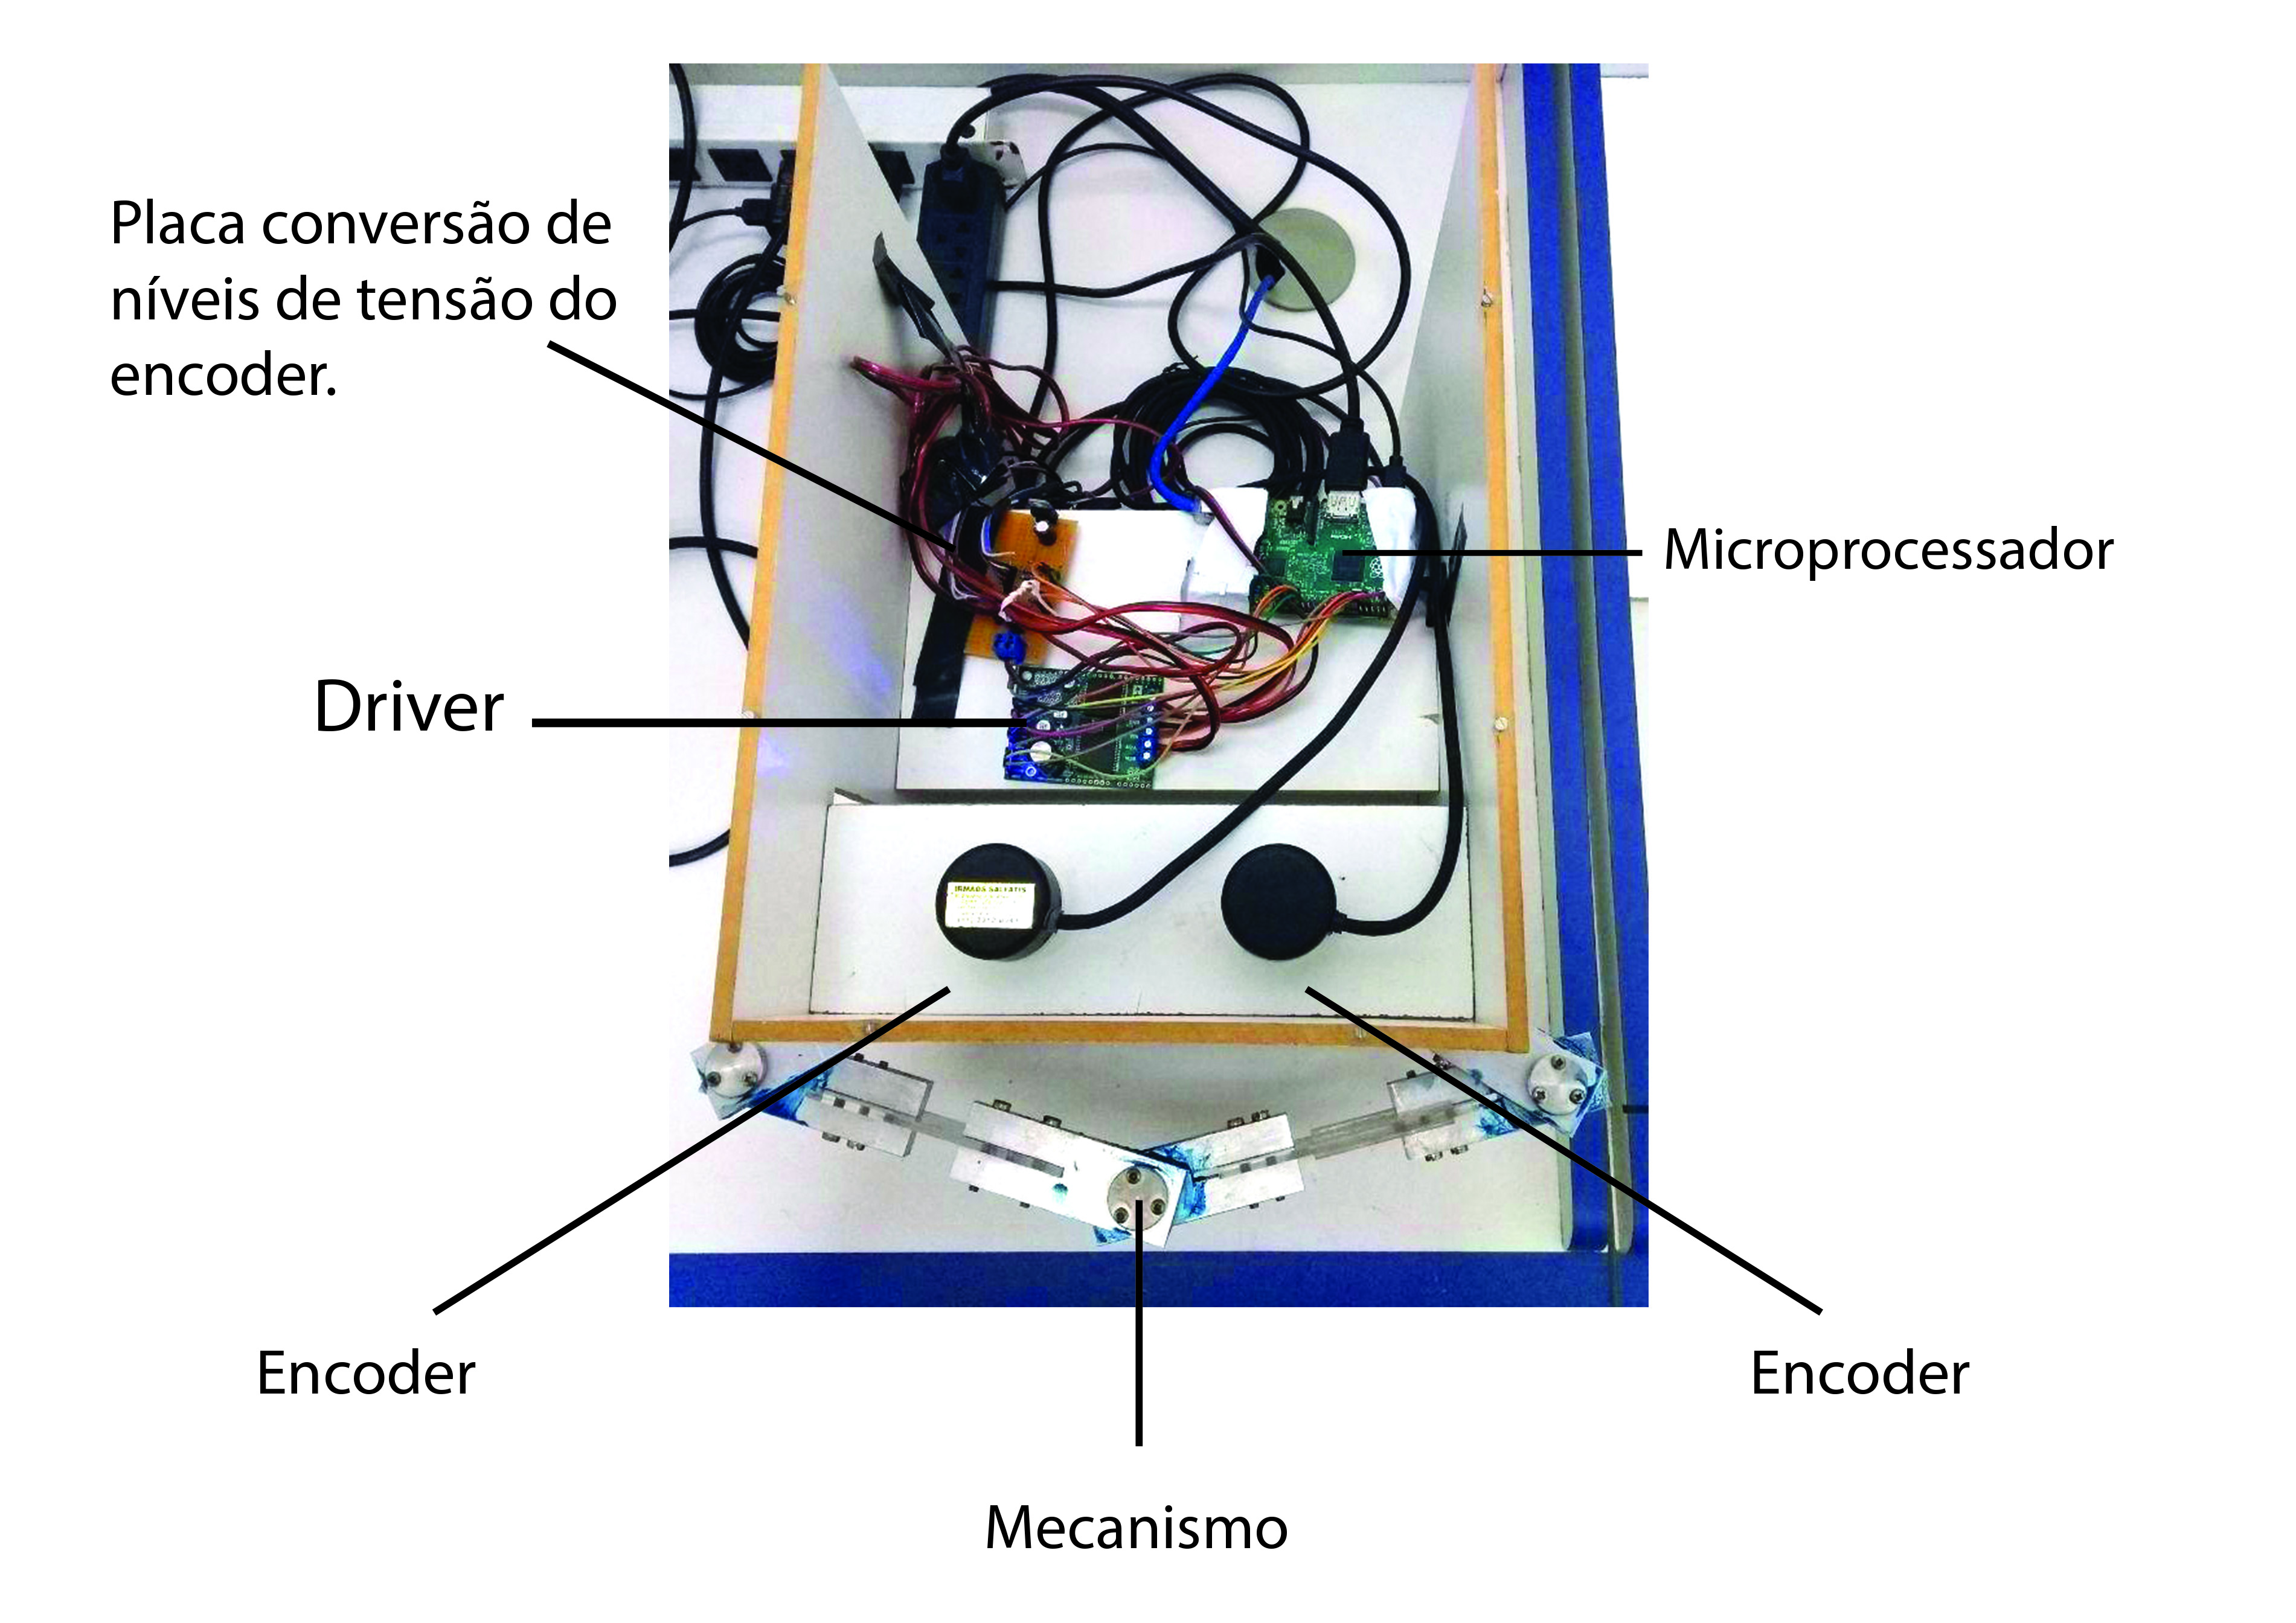
\includegraphics[scale=0.1]{imagens/BancadaClara1.jpg}
    \caption{Bancada experimental}
    \label{fig:BancadaClara1}
\end{figure}

%\begin{figure}[H]
%    \centering
%    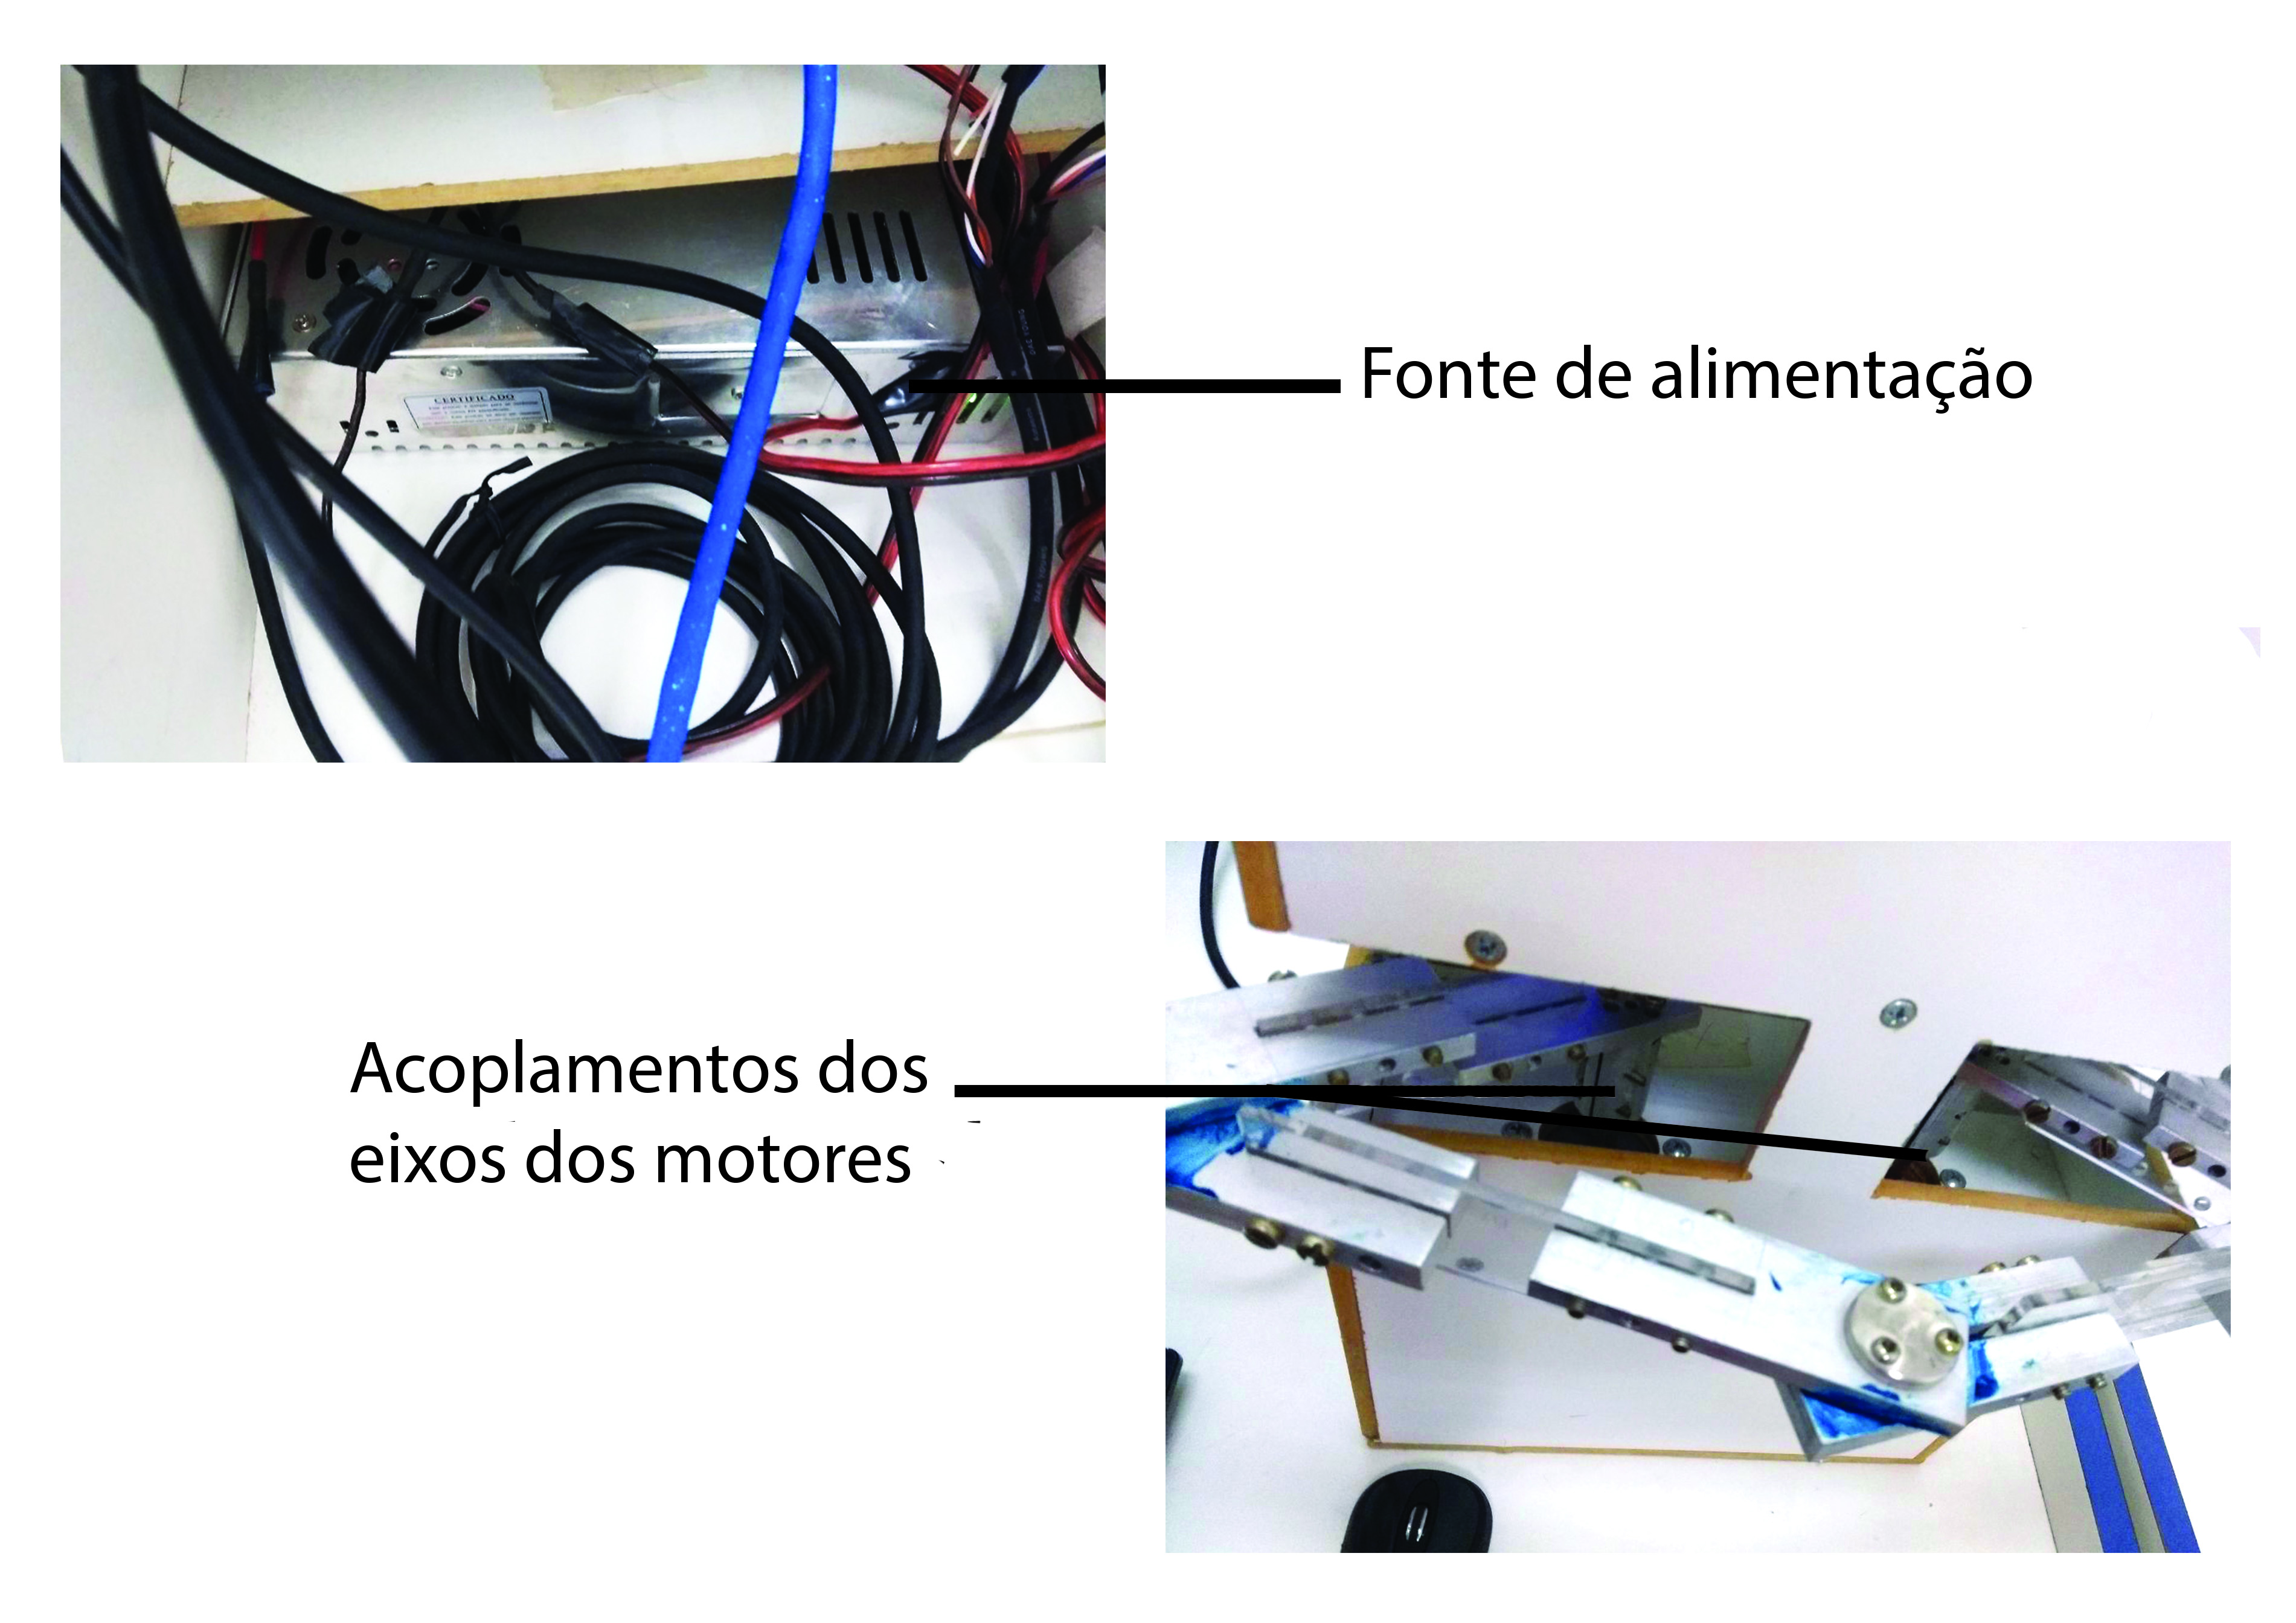
\includegraphics[scale=0.1]{imagens/BancadaClara2.jpg}
%    \caption{Arquitetura do sistema}
%    \label{arquitSistema2}
%\end{figure}

\subsection{Sistema de controle}

O sistema de controle é constituído de: 
\begin{itemize}
\item Derivadores numéricos para a obtencão da velocidade e aceleração dos motores
\item Observadores das correntes que passam pelos motores
\item Malhas de controles (malha de controle de corrente e malha de controle de posição) 
\end{itemize} 

Pelos enconders são obtidos os deslocamentos angulares dos motores, e com os derivadores numéricos são obtidos seus sinais de velocidade e acelaração. Esses três sinais juntos com suas respectivas referências são utilizados na malha de controle de posição. Os sinais de velocidade e de tensão que são enviados aos motores são utilizados para estimar as correntes que passam pelos motores. A partir dos erros entre o valores estimados e as correntes de referência, o controlador calcula, a partir da lei de controle, as tensões a serem enviadas aos motores. Representações das arquiteturas de controle implementadas, controle no espaço das juntas e no espaço da tarefa, podem ser vistas nas figuras \ref{fig:ControleEspacoDasJuntas} e \ref{fig:ControleEspacoDaTarefa}.

\begin{figure}[H]
    \centering
    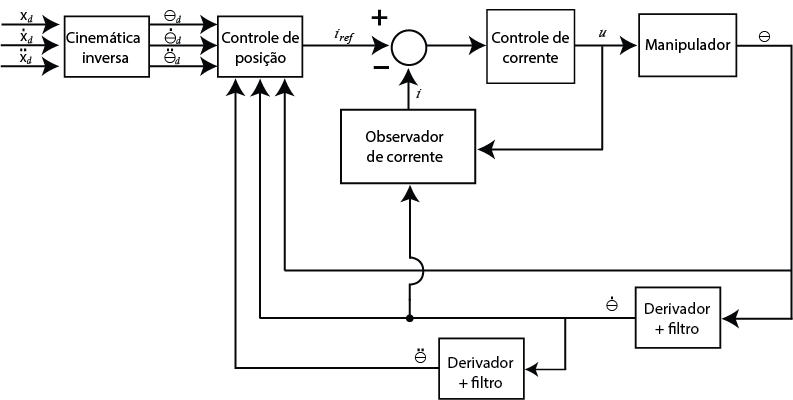
\includegraphics[scale=0.5]{imagens/ControleEspacoDasJuntas.png}
    \caption{Arquitetura de controle: espaço das juntas}
    \label{fig:ControleEspacoDasJuntas}
\end{figure}

\begin{figure}[H]
    \centering
    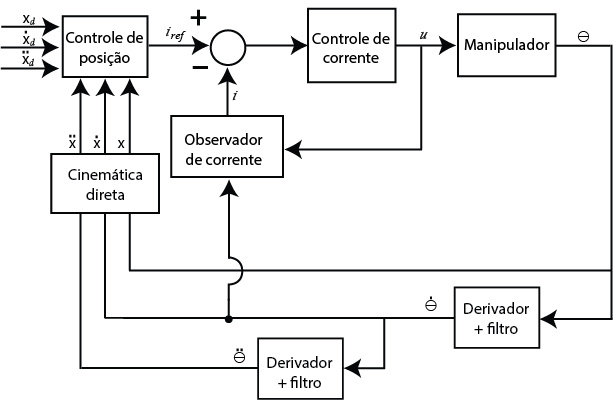
\includegraphics[scale=0.5]{imagens/ControleEspacoDaTarefa.png}
    \caption{Arquitetura de controle: espaço das juntas}
    \label{fig:ControleEspacoDaTarefa}
\end{figure}

\subsection{Derivadores numéricos}
\label{derivador}

A partir das posições angulares obtidas através da leitura dos encoders, é possível estimar as velocidades angulares dos motores utilizando um derivador numérico. Uma das formas de se implementar um derivador numérico é utilizar o método das diferenças finitas:

\begin{equation}
\dot{x}_k = \frac{x_k - x_{k-1}}{T}
\end{equation}

No entanto, como há ruídos nos sinais obtidos, a utilização  do método das diferenças finitas amplifica os ruídos de alta frequência. Diante disso, os derivadores numéricos foram utilizados em série com filtros passa-baixa tipo Bessel de segunda ordem (para a estimação da velocidade a partir da posição) e oitava ordem (para a estimação da aceleração a partir da velocidade).

\subsection{Observador de corrente}

Para a estimação da corrente elétrica foi considerada a equacação da dinâmica elétrica do motor \eqref{eq:DinEletrica_rot}:

\begin{equation}
\tag{\ref{eq:DinEletrica_rot}} \label{eq:DinamicaEletricaMotor}
	   u = L \frac{di}{dt} + R i + k_{e} \omega
\end{equation}

Esta equação pode interpretada como um sistema linear de primeira ordem com entrada $u - k_{e} \omega $ e polo em $s = -R/L$. Sendo assim, o sistema pode ser considerado naturalmente estável e pode ser utilizado um observador em malha aberta para estimar a corrente elétrica.

Tendo em vista que a frequencia do polo deste sistema está em torno de 240Hz, muito acima das frequências em que o sistema mecânico opera, o observador de corrente é implementado simplemente a partir do cálculo da corrente considerando a equação \eqref{eq:DinamicaEletricaMotor} em regime permanente, ou seja, $\frac{di}{dt} = 0$. Com isso, obtemos a seguinte expressão para o observador de corrente:

\begin{equation}
\label{corrente}
\hat{i} = \frac{u - k_e \omega}{R}
\end{equation}

\subsection{Compensadores de não-linearidades}

Para implementar as técnicas de controle baseadas em modelo, é utilizado o algoritmo de modelagem proposto para tabelar os termos do modelo dinâmico que dependem apenas da posição.

Tendo em vista que a matriz de inércia generalizada depende apenas da posição, e que a matriz-coluna de esforços de inérciais giroscópicos pode ser expressa como a soma de matrizes coluna dependentes apenas da posição multiplicados por termos quadráticos das quasi-velocidades independentes, é feita uma discretização da área de trabalho, de modo a calcular o valor destas matrizes em um número finito de pontos e realizar interpolações em tempo real, de modo a obter um valor estimado desses termos da dinâmica em qualquer ponto não singular pertencente à area de trabalho.

A discretização realizada aplica uma malha quadradiculada de lado $5mm$ na área de trabalho do mecanismo, de modo a calcular os termos da dinâmica comentados em cada ponto não singular pertencente à discretização.

\subsection{Estratégias de controle}

Foram realizados ensaios experimentais utilizando as seguintes estratégias de controle:

\begin{itemize}
\item Controle Proporcial-Derivativo com pré-alimentação no espaço das juntas (PDq)
\item Controle Proporcial-Derivativo com pré-alimentação no espaço da tarefa (PDx)
\item Controle por Toque Computado no espaço das juntas (TCq)
\item Controle por Toque Computado no espaço da tarefa (TCx)
\item Controle Proporcial-Derivativo + Modos Deslizantes no espaço das juntas (PDMDq)
\item Controle Proporcial-Derivativo + Modos Deslizantes no espaço da tarefa (PDMDx)
\item Controle por Toque Computado + Modos Deslizantes no espaço das juntas (TCMDq)
\item Controle por Toque Computado + Modos Deslizantes no espaço da tarefa (TCMDx)
\end{itemize}

Todas as leis de controle podem ser obtidas através da seguinte lei de controle, deduzida em \ref{sec:CMD}:
\begin{equation}
\mu' = \hat{\mH} \cdot \Big(\ddot{\mxi}_d + \underline{k}_v \dot{\me} + \underline{k}_p \me + \int_0^t \underline{k} \, \sat(\ms/\phi)\,d \tau \Big) + \hat{\mh}
\end{equation}
Sendo:
\begin{equation}
\ms = \ddot{\me} + \underline{k}_v \dot{\me} + \underline{k}_p \me
\end{equation}

Repare que, para $\underline{k} = \mzr$, temos a lei de Controle por Torque Computado. Para $\underline{k} = \mzr$, $\hat{\mh} = \mzr$ e $\hat{\mH}$ constante e diagonal, temos uma lei de Controle Proporcional-Derivativo com pré-alimentação. Sendo assim, para $\underline{k} \neq \mzr$, podemos obter estas mesmas leis de controle, agora com um termo adicional de controle robusto vindo do Controle por Modos Deslizantes.

Esta lei de controle tem a vantagem de, além de poder ser interpretada como uma estratégia híbrida, praticamente elimina o fenômeno do \emph{chattering}, tendo em vista que o termo descontínuo é suavizado através de uma função de saturação e uma integral.

\subsection{Parâmetros do sistema}

Nas tabelas \ref{tab:parametrosCadeia1} e \ref{tab:parametrosCadeia2} são apresentados os valores estimados dos parâmetros das cadeias seriais do mecanismo. A massa do efetuador é considerada nula. Os comprimentos dos elos e a distância entre os atuadores são os valores de projeto do sistema e estão de acordo com as medições realizadas. Os parâmetros de inércias, ou seja, as massas, momentos de inércia, e posição dos centros de massa, foram obtidos a partir do modelo CAD do mecanismo. 

\begin{table}[H] 
\centering
\caption{Parâmetros da cadeia serial 1}
\label{tab:parametrosCadeia1}
\begin{tabular}{l|l|l}
Parâmetros   & Valores                  & Unidades      \\ \hline
$l_0$        & $0.050$                     & $m$        \\
$l_1$        & $0.120$                     & $m$        \\
$l_2$        & $0.160$                     & $m$        \\
$l_{g1}$     & $0.060$                     & $m$        \\
$l_{g2}$     & $0.078$                    & $m$        \\
$m_1$        & $0.062$                    & $kg$       \\
$m_2$        & $0.124$                    & $kg$       \\
$J_{z1}$     & $1.073 \cdot 10^{-4}$    & $kg.m^{2}$ \\
$J_{z2}$     & $4.380 \cdot 10^{-4}$    & $kg.m^{2}$ \\
\end{tabular}
\end{table} 

\begin{table}[H] 
\centering
\caption{Parâmetros da cadeia 2}
\label{tab:parametrosCadeia2}
\begin{tabular}{l|l|l}
Parâmetros   & Valores                    & Unidades   \\ \hline
$l_0$        & $0.050$                    & $m$        \\
$l_1$        & $0.120$                    & $m$        \\
$l_2$        & $0.160$                    & $m$        \\
$l_{g1}$     & $0.060$                    & $m$        \\
$l_{g2}$     & $0.058$                    & $m$        \\
$m_1$        & $0.062$                    & $kg$       \\
$m_2$        & $0.097$                    & $kg$       \\
$J_{z1}$     & $2.960   \cdot 10^{-4}$    & $kg.m^{2}$ \\
$J_{z2}$     & $9.800   \cdot 10^{-4}$    & $kg.m^{2}$ \\
\end{tabular}
\end{table}

Os valores dos parâmetros estimados dos motores são apresentados nas tabelas \ref{parametrosMotor} e \ref{parametrosMotor2}, as quais estão no apêndice \ref{ap:CurvaDosMotores}, juntamente com o processo de identificação utilizado.



\subsection{Trajetórias de referência}

A primeira trajetória realizada é uma trajetória circular com período de 1 segundo. São realizados 8 ciclos seguidos de uma parada repentina. Sua expressão é dada por:

\begin{equation}
\begin{cases}
x_d(t) = -0.05 \sin(2\pi t) \\
y_d(t) = 0.158 - 0.05 \cos(2\pi t) \\
\end{cases}
\end{equation}

A segunda trajetória a ser realizada é uma trajetória triangular cujas coordenadas dos vértices (em metros) são:

\begin{equation} \label{eq:zeroMaquina}
\mx_1 = \begin{bmatrix}
-0.002 & 0.108 
\end{bmatrix}^\msT
\end{equation}
\begin{equation}
\mx_2 = \begin{bmatrix}
0.050 & 0.258 
\end{bmatrix}^\msT
\end{equation}
\begin{equation}
\mx_3 = \begin{bmatrix}
-0.050 & 0.258 
\end{bmatrix}^\msT
\end{equation}

São realizados 2 ciclos, sendo que cada lado do triângulo é percorrido em $0.75s$, e sendo o trecho I de $\mx_1$ a $\mx_2$, o trecho II de $\mx_2$ a $\mx_3$, e o trecho III de $\mx_3$ a $\mx_1$. Depois de completar os 2 ciclos, é feita uma parada suave. Em cada lado do triângulo, é parametrizada uma trajetória polinomial de sétima ordem, na qual é imposta a posição inicial e final, velocidade nula, aceleração nula e tranco nulo no início e no final da trajetória. A expressão do polinômio é dada por:

\begin{equation}
\mx(\mathfrak{t}) = \mx_0 + (\mx_f - \mx_0) (35 \mathfrak{t}^4 - 84 \mathfrak{t}^5 + 70 \mathfrak{t}^6 - 20 \mathfrak{t}^7)
\end{equation}

Sendo $\mx$ a posição atual, $\mx_0$ a posição inicial, $\mx_f$ a posição final, e $\mathfrak{t}$ a fração do tempo decorrido em relação ao tempo total da trajetória (repare que $\mx(1) = \mx_f$).

\subsection{Condições iniciais}

O mecanismo sempre parte do repouso na posição $\mx_1$, dada pela equação \eqref{eq:zeroMaquina}

\begin{equation} \label{eq:zeroMaquina}
\mx_1 = \begin{bmatrix}
-0.002 & 0.108 
\end{bmatrix}^\msT
\end{equation}

\subsection{Parâmetros dos controladores}

Com o intuito de que o sistema em malha fechada se comporte como um sistema de segunda ordem com amortecimento crítico, $\underline{k}_p$ e $\underline{k}_v$ são parametrizados em função de um parâmetro $\lambda$, da seguinte maneira:
\begin{equation}
\underline{k}_p = \lambda^2 \mone
\end{equation}
\begin{equation}
\underline{k}_v = 2 \lambda \mone
\end{equation}

Os parâmetros dos controladores de posição utilizados nas trajetórias definidas são apresentados nas tabelas \ref{tab:parametrosControleAtuadoresCirculo}, \ref{tab:parametrosControleAtuadoresTriangulo} e \ref{tab:parametrosControleEfetuador}.

\begin{table}[H] 
\centering
\caption{Parâmetros dos controladores: espaço das juntas - trajetória circular}
\label{tab:parametrosControleAtuadoresCirculo}
\begin{tabular}{l|l|l|l|l|l}
Estratégia & $\lambda [rad/s]$  & $m^*[kg.m^2]$ & $\phi[rad/s^2]$   & $k_1[rad/s^2]$ & $k_2[rad/s^2]$ \\ \hline
PDq        & $35$               & $3.58 \cdot 10^{-3}$  & -         & -              & -              \\
PDMDq      & $35$               & $3.58 \cdot 10^{-3}$  & $20$      & $200$          & $200$          \\
TCq        & $60$               & -                     & -         & -              & -              \\
TCMDq      & $60$               & -                     & $20$      & $363$          & $363$          \\
\end{tabular}
\end{table}

\begin{table}[H] 
\centering
\caption{Parâmetros dos controladores: espaço das juntas - trajetória triangular}
\label{tab:parametrosControleAtuadoresTriangulo}
\begin{tabular}{l|l|l|l|l|l}
Estratégia & $\lambda [rad/s]$  & $m^*[kg.m^2]$         & $\phi[rad/s^2]$   & $k_1[rad/s^2]$ & $k_2[rad/s^2]$ \\ \hline
PDq        & $25$               & $3.58 \cdot 10^{-3}$  & -         & -              & -              \\
PDMDq      & $25$               & $3.58 \cdot 10^{-3}$  & $90$      & $200$          & $200$          \\
TCq        & $60$               & -                     & -         & -              & -              \\
TCMDq      & $60$               & -                     & $20$      & $363$          & $363$          \\
\end{tabular}
\end{table}

\begin{table}[H] 
\centering
\caption{Parâmetros dos controladores: espaço da tarefa}
\label{tab:parametrosControleEfetuador}
\begin{tabular}{l|l|l|l|l|l}
Estratégia & $\lambda [rad/s]$  & $m^*[kg]$ & $\phi[m/s^2]$ & $k_1[m/s^2]$ & $k_2[m/s^2]$ \\ \hline
PDx        & $70$               & $0.207$   & -             & -            & -            \\
PDMDx      & $70$               & $0.207$   & $6$           & $70$         & $0$          \\
TCx        & $60$               & -         & -             & -            & -            \\
TCMDx      & $60$               & -         & $6$           & $103$        & $0$          \\
\end{tabular}
\end{table}

Além disso, os controladores de corrente utilizados são controladores lineares de segunda ordem, projetados por alocação de polos. A expressões das funções de transferência de um motor DC são deduzidas e apresentadas no apêndice \ref{ap:FuncoesDeTransferencia}, e o projeto do controlador é apresentado no apêndice \ref{ap:ControladorDeCorrente}. Tendo em vista que o período de amostragem da malha de corrente é de $1ms$, 3 dos pólos 4 polos da malha de corrente são alocados em $z=0$, $z=0.6$, $z=0.7$. O último polo é alocado na mesma posição do zero em malha aberta do sistema.

\subsection{Resultados experimentais}

Nesta subsessão são apresentados os gráficos de seguimento de trajetória, da evolução temporal dos erros de controle em $x$ e $y$, e da evolução temporal dos esforços de controle para todas as 8 estratégias de controle definidas, tanto para a trajetória circular, quanto para a trajetória triangular (figuras de \ref{fig:PIDq_circulo_xy} a \ref{fig:SMCx_triangulo_tau2}). Também são apresentadas tabelas de comparação de desempenho e é feita a discussão dos resultados.

\newpage

\subsubsection{PDq - Trajetória circular}

\begin{figure}[H]
	\centering
	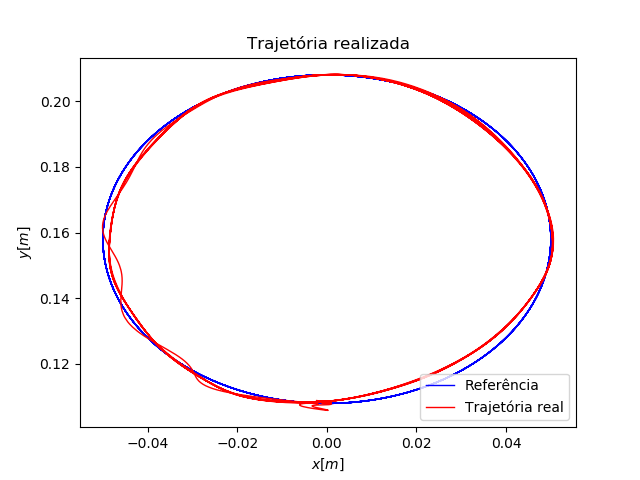
\includegraphics[scale=0.39]{../../../Experimental/Aquisicoes/PIDt_circulo/xy.png}  
	\caption{Trajetória realizada}
	\label{fig:PIDq_circulo_xy}
\end{figure}
\begin{multicols}{2}
\begin{figure}[H]
	\centering
	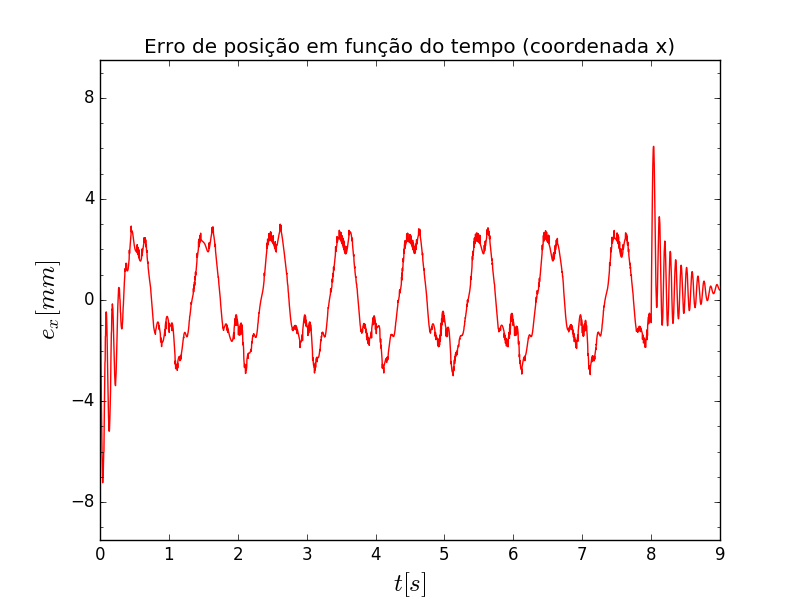
\includegraphics[scale=0.39]{../../../Experimental/Aquisicoes/PIDt_circulo/ex.png}  
	\caption{Erro de controle $e_x$}
	\label{fig:PIDq_circulo_ex}
\end{figure}
\begin{figure}[H]
	\centering
	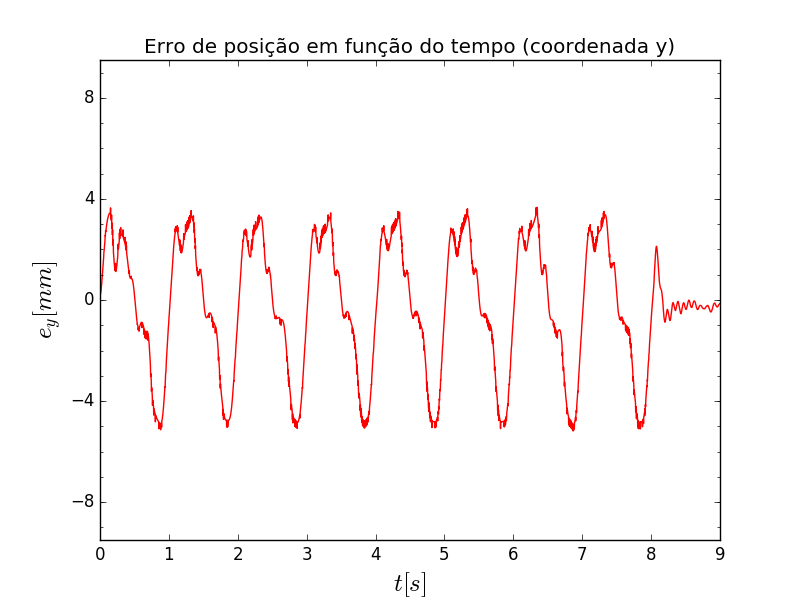
\includegraphics[scale=0.39]{../../../Experimental/Aquisicoes/PIDt_circulo/ey.png}  
	\caption{Erro de controle $e_y$}
	\label{fig:PIDq_circulo_ey}
\end{figure}
\end{multicols}
\begin{multicols}{2}
\begin{figure}[H]
	\centering
	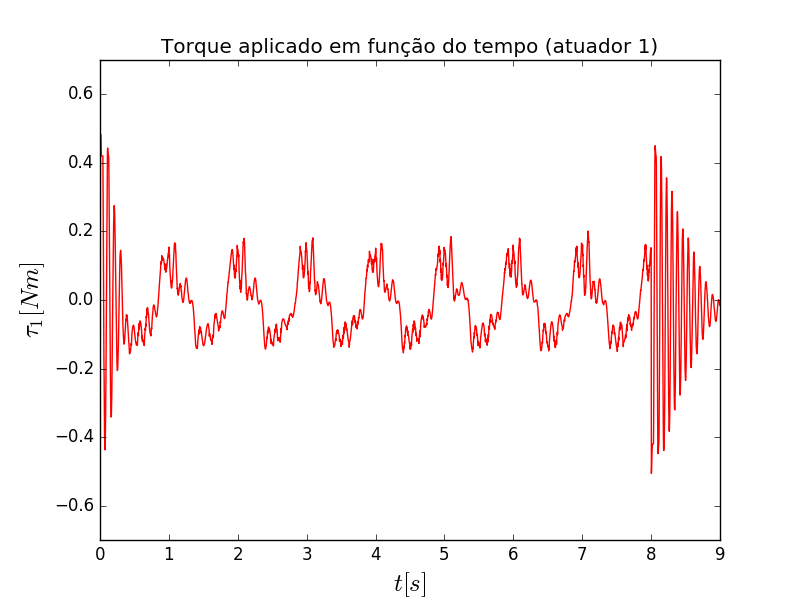
\includegraphics[scale=0.39]{../../../Experimental/Aquisicoes/PIDt_circulo/tau1.png}  
	\caption{Esforço de controle $\tau_1$}
	\label{fig:PIDq_circulo_tau1}
\end{figure}
\begin{figure}[H]
	\centering
	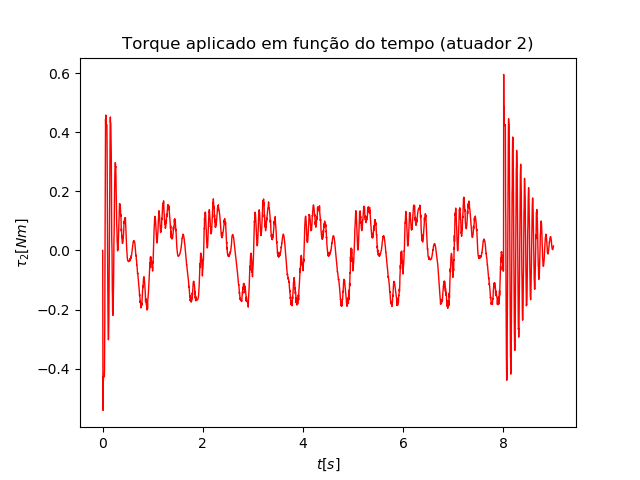
\includegraphics[scale=0.39]{../../../Experimental/Aquisicoes/PIDt_circulo/tau2.png}  
	\caption{Esforço de controle $\tau_2$}
	\label{fig:PIDq_circulo_tau2}
\end{figure}
\end{multicols}

\subsubsection{PDMDq - Trajetória circular}

\begin{figure}[H]
	\centering
	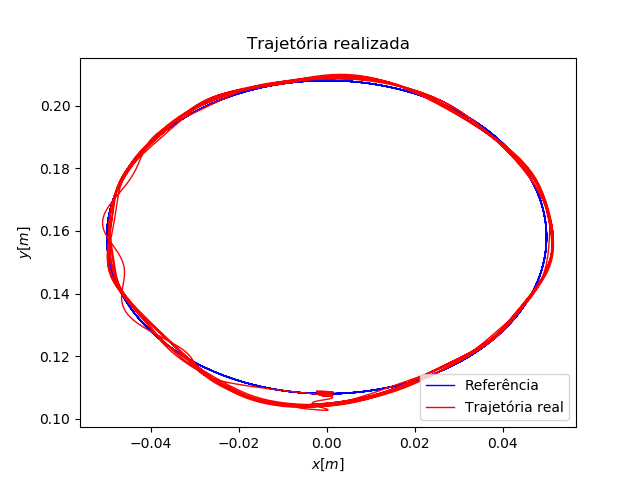
\includegraphics[scale=0.39]{../../../Experimental/Aquisicoes/PIDSMCt_circulo/xy.png}  
	\caption{Trajetória realizada}
	\label{fig:PIDSMCq_circulo_xy}
\end{figure}
\begin{multicols}{2}
\begin{figure}[H]
	\centering
	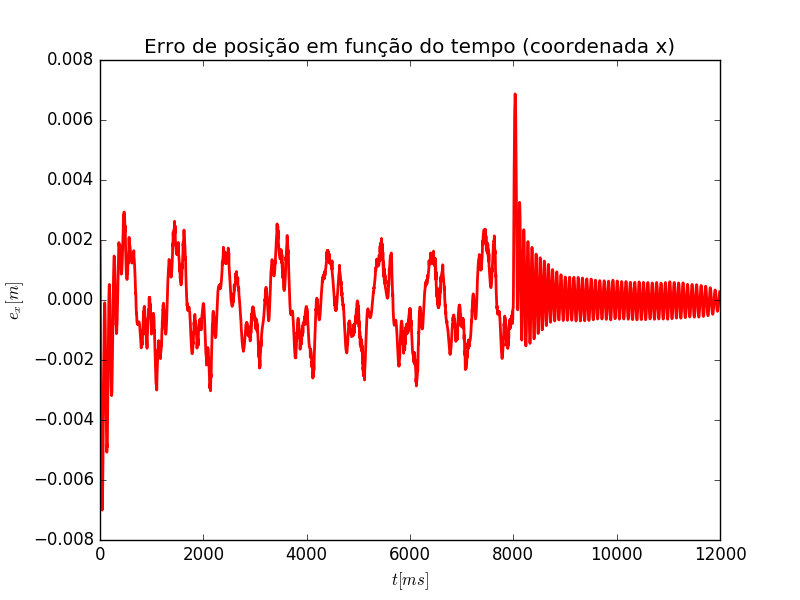
\includegraphics[scale=0.39]{../../../Experimental/Aquisicoes/PIDSMCt_circulo/ex.png}  
	\caption{Erro de controle $e_x$}
	\label{fig:PIDSMCq_circulo_ex}
\end{figure}
\begin{figure}[H]
	\centering
	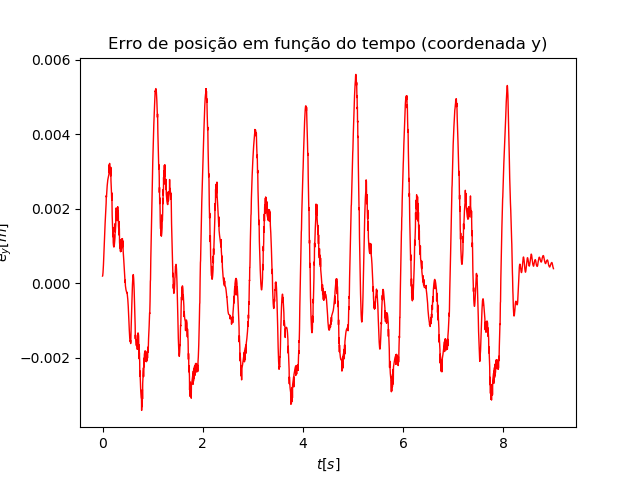
\includegraphics[scale=0.39]{../../../Experimental/Aquisicoes/PIDSMCt_circulo/ey.png}  
	\caption{Erro de controle $e_y$}
	\label{fig:PIDSMCq_circulo_ey}
\end{figure}
\end{multicols}
\begin{multicols}{2}
\begin{figure}[H]
	\centering
	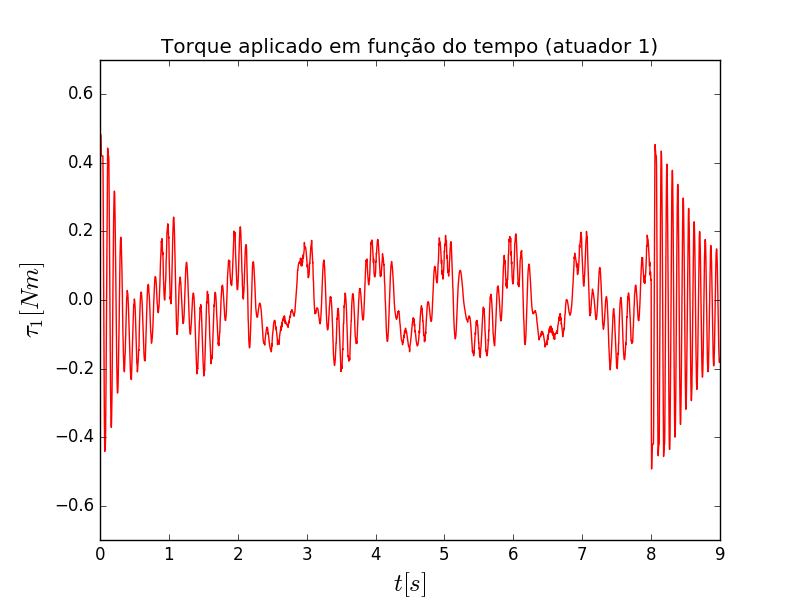
\includegraphics[scale=0.39]{../../../Experimental/Aquisicoes/PIDSMCt_circulo/tau1.png}  
	\caption{Esforço de controle $\tau_1$}
	\label{fig:PIDSMCq_circulo_tau1}
\end{figure}
\begin{figure}[H]
	\centering
	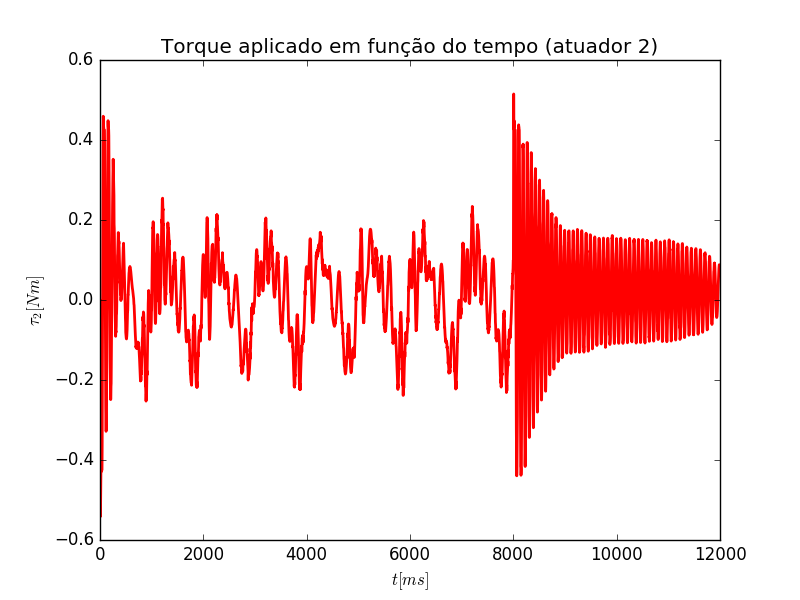
\includegraphics[scale=0.39]{../../../Experimental/Aquisicoes/PIDSMCt_circulo/tau2.png}  
	\caption{Esforço de controle $\tau_2$}
	\label{fig:PIDSMCq_circulo_tau2}
\end{figure}
\end{multicols}

\subsubsection{TCq - Trajetória circular}

\begin{figure}[H]
	\centering
	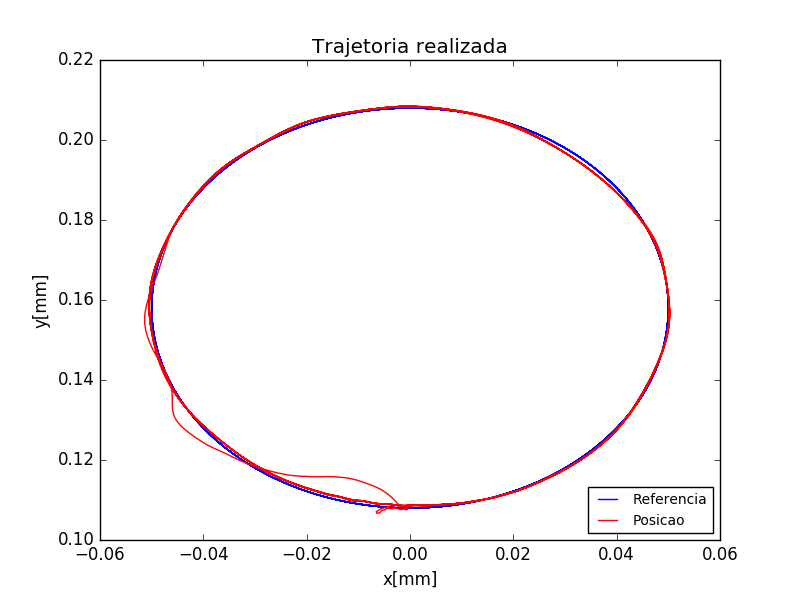
\includegraphics[scale=0.39]{../../../Experimental/Aquisicoes/CTCt_circulo/xy.png}  
	\caption{Trajetória realizada}
	\label{fig:CTCq_circulo_xy}
\end{figure}
\begin{multicols}{2}
\begin{figure}[H]
	\centering
	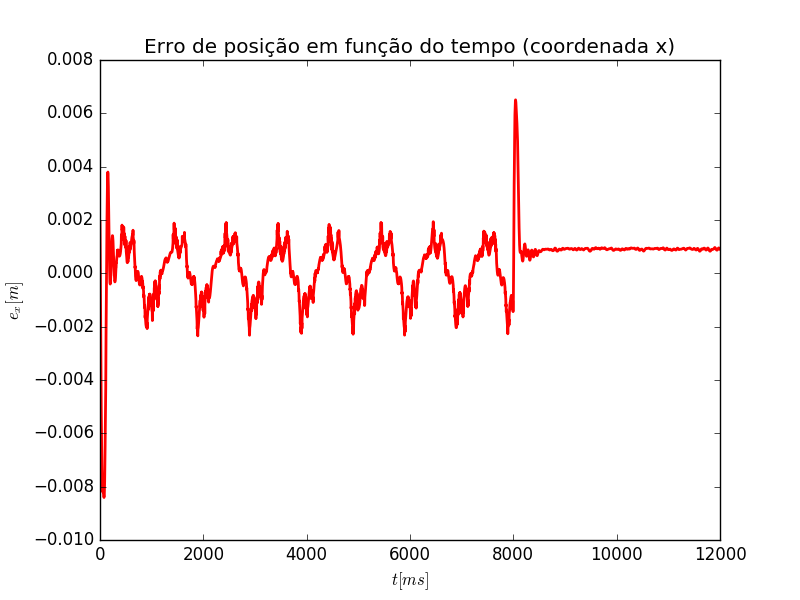
\includegraphics[scale=0.39]{../../../Experimental/Aquisicoes/CTCt_circulo/ex.png}  
	\caption{Erro de controle $e_x$}
	\label{fig:CTCq_circulo_ex}
\end{figure}
\begin{figure}[H]
	\centering
	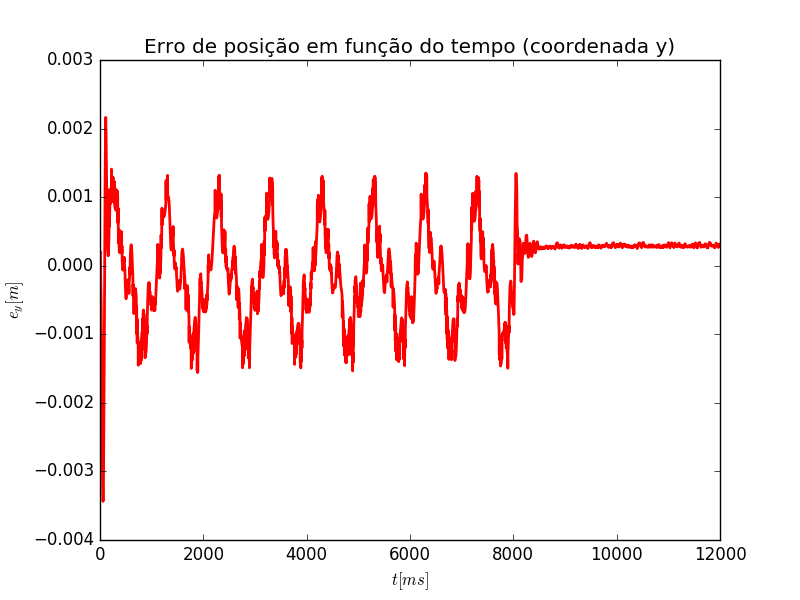
\includegraphics[scale=0.39]{../../../Experimental/Aquisicoes/CTCt_circulo/ey.png}  
	\caption{Erro de controle $e_y$}
	\label{fig:CTCq_circulo_ey}
\end{figure}
\end{multicols}
\begin{multicols}{2}
\begin{figure}[H]
	\centering
	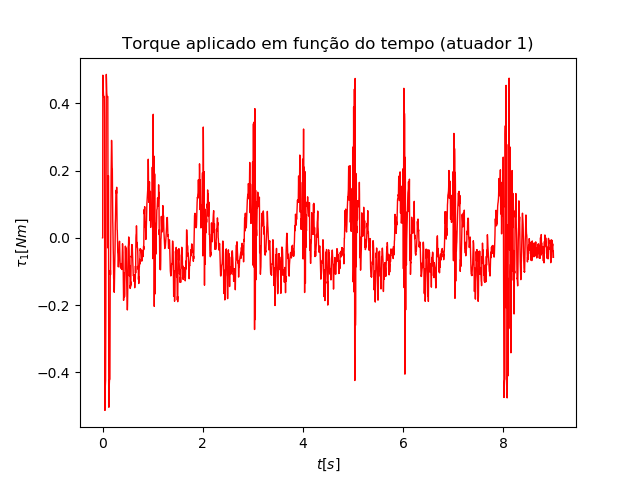
\includegraphics[scale=0.39]{../../../Experimental/Aquisicoes/CTCt_circulo/tau1.png}  
	\caption{Esforço de controle $\tau_1$}
	\label{fig:CTCq_circulo_tau1}
\end{figure}
\begin{figure}[H]
	\centering
	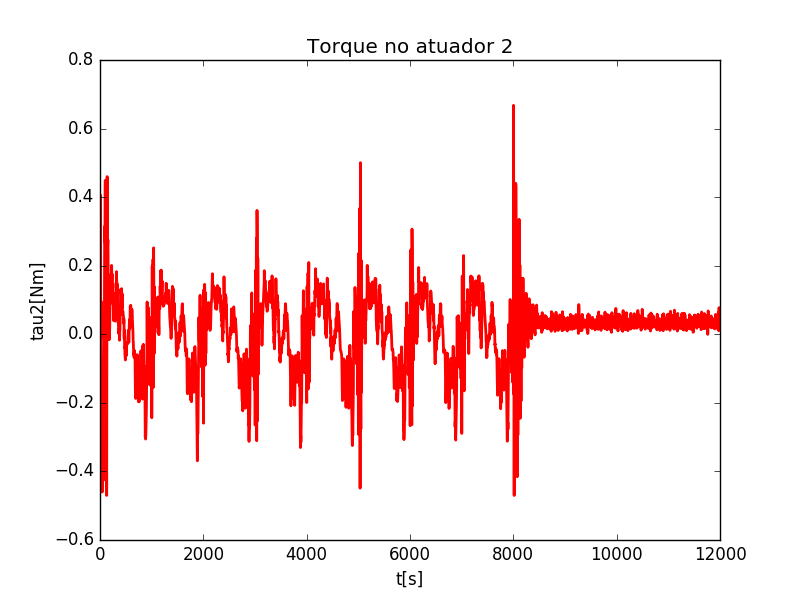
\includegraphics[scale=0.39]{../../../Experimental/Aquisicoes/CTCt_circulo/tau2.png}  
	\caption{Esforço de controle $\tau_2$}
	\label{fig:CTCq_circulo_tau2}
\end{figure}
\end{multicols}

\subsubsection{TCMDq - Trajetória circular}

\begin{figure}[H]
	\centering
	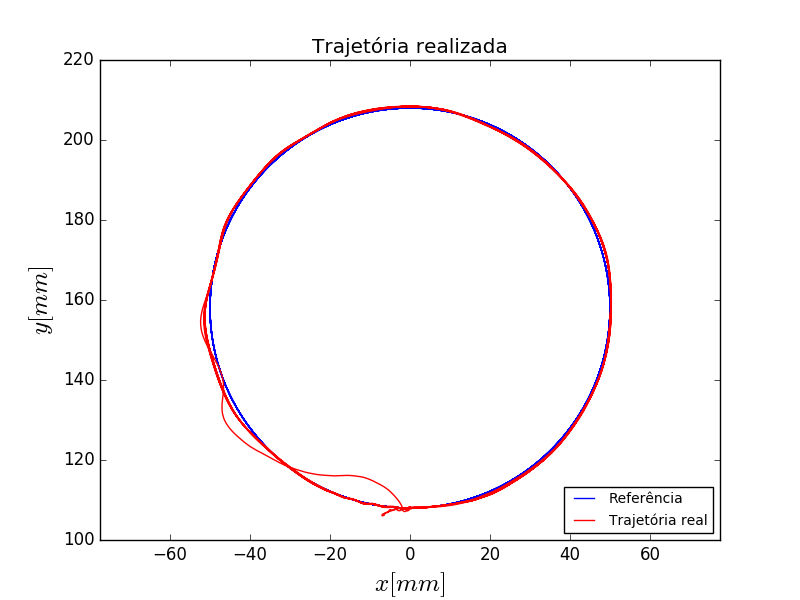
\includegraphics[scale=0.39]{../../../Experimental/Aquisicoes/SMCt_circulo/xy.png}  
	\caption{Trajetória realizada}
	\label{fig:SMCq_circulo_xy}
\end{figure}
\begin{multicols}{2}
\begin{figure}[H]
	\centering
	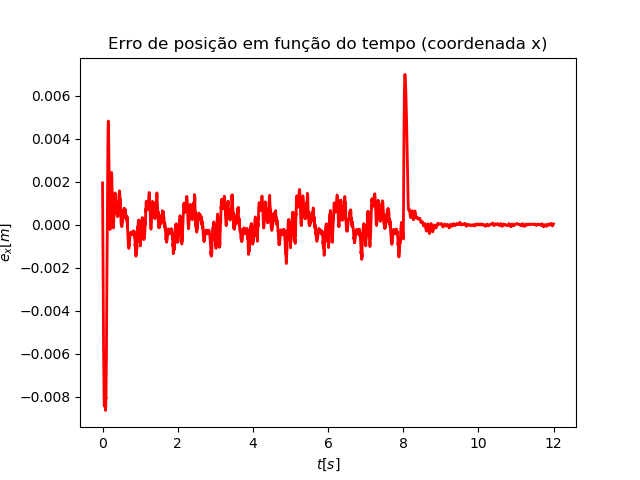
\includegraphics[scale=0.39]{../../../Experimental/Aquisicoes/SMCt_circulo/ex.png}  
	\caption{Erro de controle $e_x$}
	\label{fig:SMCq_circulo_ex}
\end{figure}
\begin{figure}[H]
	\centering
	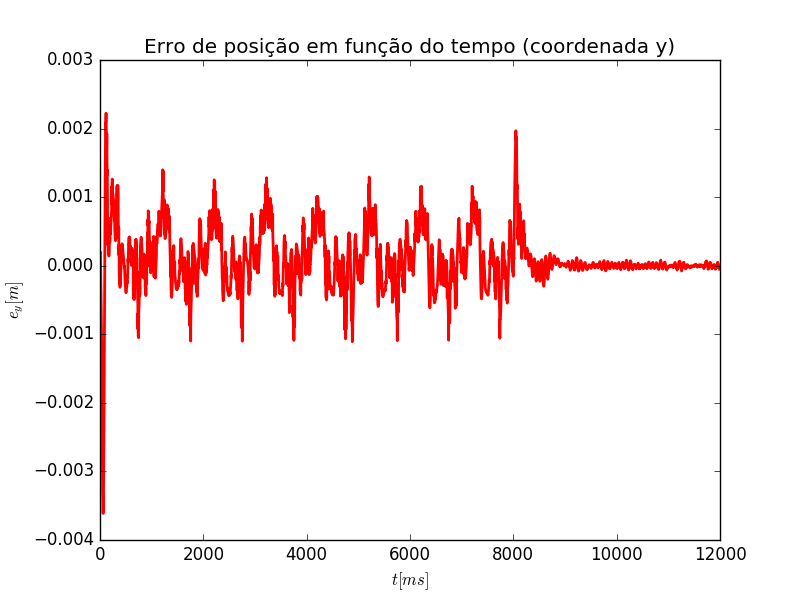
\includegraphics[scale=0.39]{../../../Experimental/Aquisicoes/SMCt_circulo/ey.png}  
	\caption{Erro de controle $e_y$}
	\label{fig:SMCq_circulo_ey}
\end{figure}
\end{multicols}
\begin{multicols}{2}
\begin{figure}[H]
	\centering
	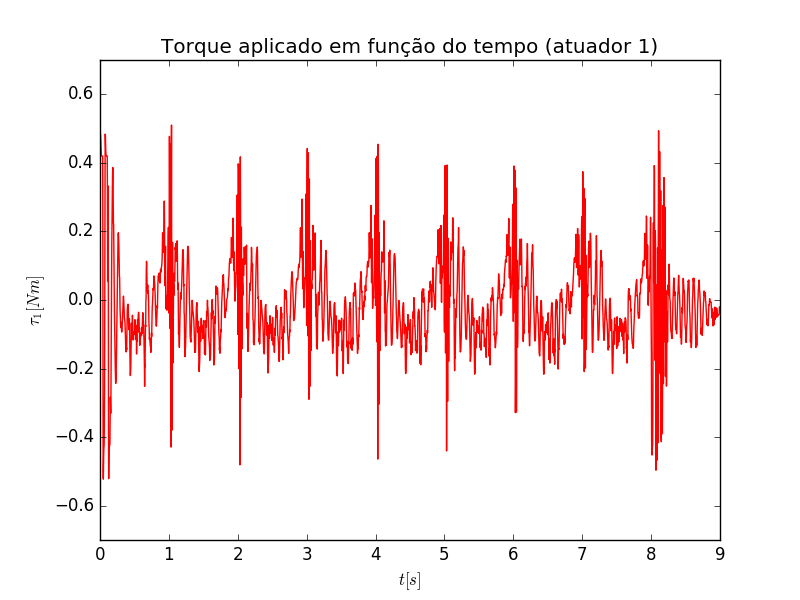
\includegraphics[scale=0.39]{../../../Experimental/Aquisicoes/SMCt_circulo/tau1.png}  
	\caption{Esforço de controle $\tau_1$}
	\label{fig:SMCq_circulo_tau1}
\end{figure}
\begin{figure}[H]
	\centering
	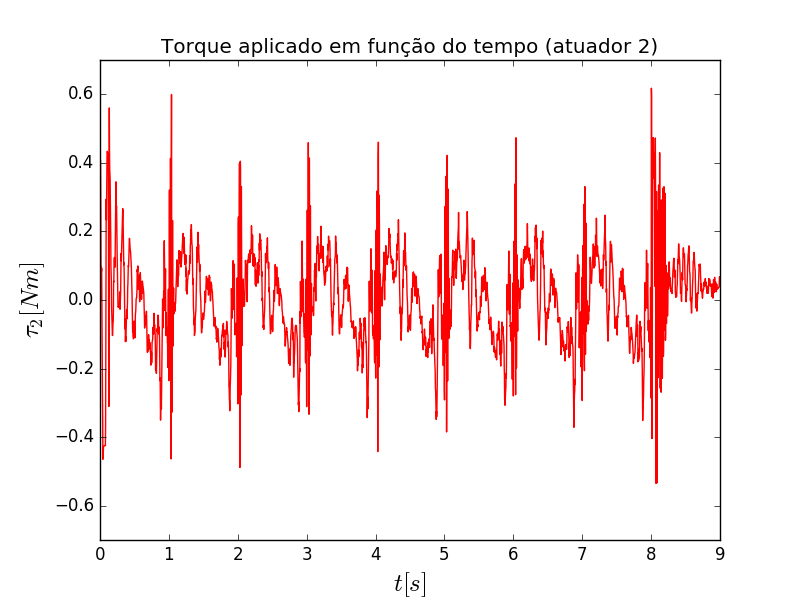
\includegraphics[scale=0.39]{../../../Experimental/Aquisicoes/SMCt_circulo/tau2.png}  
	\caption{Esforço de controle $\tau_2$}
	\label{fig:SMCq_circulo_tau2}
\end{figure}
\end{multicols}


\subsubsection{PDx - Trajetória circular}

\begin{figure}[H]
	\centering
	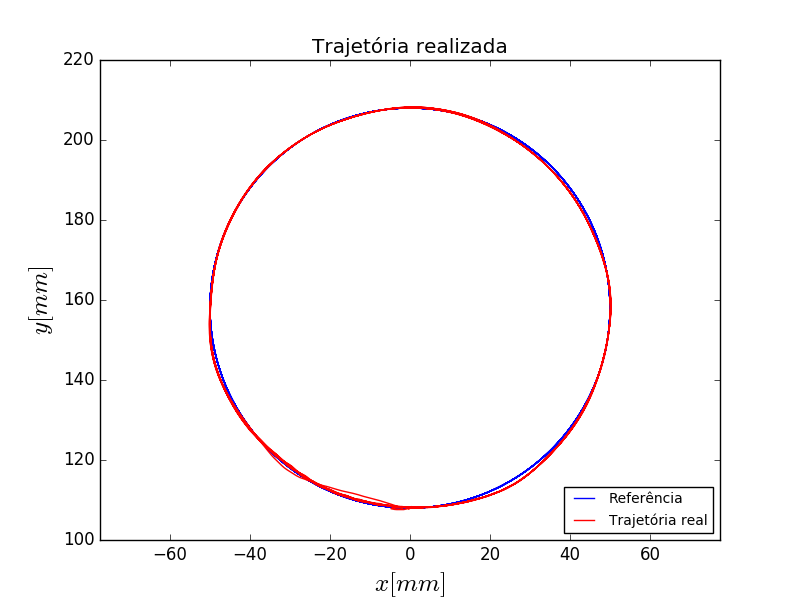
\includegraphics[scale=0.39]{../../../Experimental/Aquisicoes/PIDx_circulo/xy.png}  
	\caption{Trajetória realizada}
	\label{fig:PIDx_circulo_xy}
\end{figure}
\begin{multicols}{2}
\begin{figure}[H]
	\centering
	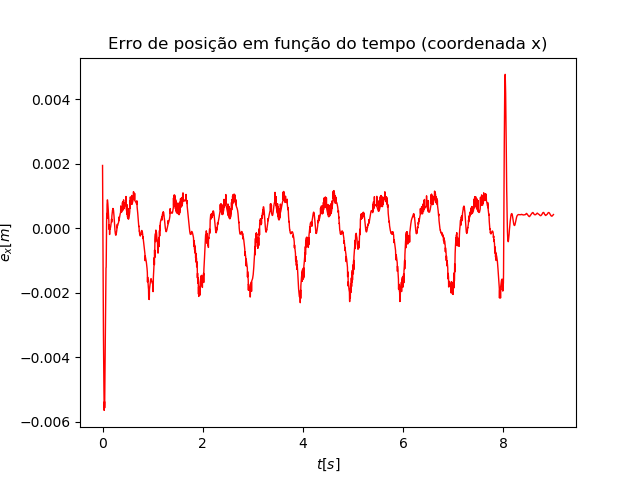
\includegraphics[scale=0.39]{../../../Experimental/Aquisicoes/PIDx_circulo/ex.png}  
	\caption{Erro de controle $e_x$}
	\label{fig:PIDx_circulo_ex}
\end{figure}
\begin{figure}[H]
	\centering
	\includegraphics[scale=0.39]{../../../Experimental/Aquisicoes/PIDx_circulo/ey.png}  
	\caption{Erro de controle $e_y$}
	\label{fig:PIDx_circulo_ey}
\end{figure}
\end{multicols}
\begin{multicols}{2}
\begin{figure}[H]
	\centering
	\includegraphics[scale=0.39]{../../../Experimental/Aquisicoes/PIDx_circulo/tau1.png}  
	\caption{Esforço de controle $\tau_1$}
	\label{fig:PIDx_circulo_tau1}
\end{figure}
\begin{figure}[H]
	\centering
	\includegraphics[scale=0.39]{../../../Experimental/Aquisicoes/PIDx_circulo/tau2.png}  
	\caption{Esforço de controle $\tau_2$}
	\label{fig:PIDx_circulo_tau2}
\end{figure}
\end{multicols}

\subsubsection{PDMDx - Trajetória circular}

\begin{figure}[H]
	\centering
	\includegraphics[scale=0.39]{../../../Experimental/Aquisicoes/PIDSMCx_circulo/xy.png}  
	\caption{Trajetória realizada}
	\label{fig:PIDSMCx_circulo_xy}
\end{figure}
\begin{multicols}{2}
\begin{figure}[H]
	\centering
	\includegraphics[scale=0.39]{../../../Experimental/Aquisicoes/PIDSMCx_circulo/ex.png}  
	\caption{Erro de controle $e_x$}
	\label{fig:PIDSMCx_circulo_ex}
\end{figure}
\begin{figure}[H]
	\centering
	\includegraphics[scale=0.39]{../../../Experimental/Aquisicoes/PIDSMCx_circulo/ey.png}  
	\caption{Erro de controle $e_y$}
	\label{fig:PIDSMCx_circulo_ey}
\end{figure}
\end{multicols}
\begin{multicols}{2}
\begin{figure}[H]
	\centering
	\includegraphics[scale=0.39]{../../../Experimental/Aquisicoes/PIDSMCx_circulo/tau1.png}  
	\caption{Esforço de controle $\tau_1$}
	\label{fig:PIDSMCx_circulo_tau1}
\end{figure}
\begin{figure}[H]
	\centering
	\includegraphics[scale=0.39]{../../../Experimental/Aquisicoes/PIDSMCx_circulo/tau2.png}  
	\caption{Esforço de controle $\tau_2$}
	\label{fig:PIDSMCx_circulo_tau2}
\end{figure}
\end{multicols}

\subsubsection{TCx - Trajetória circular}

\begin{figure}[H]
	\centering
	\includegraphics[scale=0.39]{../../../Experimental/Aquisicoes/CTCx_circulo/xy.png}  
	\caption{Trajetória realizada}
	\label{fig:CTCx_circulo_xy}
\end{figure}
\begin{multicols}{2}
\begin{figure}[H]
	\centering
	\includegraphics[scale=0.39]{../../../Experimental/Aquisicoes/CTCx_circulo/ex.png}  
	\caption{Erro de controle $e_x$}
	\label{fig:CTCx_circulo_ex}
\end{figure}
\begin{figure}[H]
	\centering
	\includegraphics[scale=0.39]{../../../Experimental/Aquisicoes/CTCx_circulo/ey.png}  
	\caption{Erro de controle $e_y$}
	\label{fig:CTCx_circulo_ey}
\end{figure}
\end{multicols}
\begin{multicols}{2}
\begin{figure}[H]
	\centering
	\includegraphics[scale=0.39]{../../../Experimental/Aquisicoes/CTCx_circulo/tau1.png}  
	\caption{Esforço de controle $\tau_1$}
	\label{fig:CTCx_circulo_tau1}
\end{figure}
\begin{figure}[H]
	\centering
	\includegraphics[scale=0.39]{../../../Experimental/Aquisicoes/CTCx_circulo/tau2.png}  
	\caption{Esforço de controle $\tau_2$}
	\label{fig:CTCx_circulo_tau2}
\end{figure}
\end{multicols}

\subsubsection{TCMDx - Trajetória circular}

\begin{figure}[H]
	\centering
	\includegraphics[scale=0.39]{../../../Experimental/Aquisicoes/SMCx_circulo/xy.png}  
	\caption{Trajetória realizada}
	\label{fig:SMCx_circulo_xy}
\end{figure}
\begin{multicols}{2}
\begin{figure}[H]
	\centering
	\includegraphics[scale=0.39]{../../../Experimental/Aquisicoes/SMCx_circulo/ex.png}  
	\caption{Erro de controle $e_x$}
	\label{fig:SMCx_circulo_ex}
\end{figure}
\begin{figure}[H]
	\centering
	\includegraphics[scale=0.39]{../../../Experimental/Aquisicoes/SMCx_circulo/ey.png}  
	\caption{Erro de controle $e_y$}
	\label{fig:SMCx_circulo_ey}
\end{figure}
\end{multicols}
\begin{multicols}{2}
\begin{figure}[H]
	\centering
	\includegraphics[scale=0.39]{../../../Experimental/Aquisicoes/SMCx_circulo/tau1.png}  
	\caption{Esforço de controle $\tau_1$}
	\label{fig:SMCx_circulo_tau1}
\end{figure}
\begin{figure}[H]
	\centering
	\includegraphics[scale=0.39]{../../../Experimental/Aquisicoes/SMCx_circulo/tau2.png}  
	\caption{Esforço de controle $\tau_2$}
	\label{fig:SMCx_circulo_tau2}
\end{figure}
\end{multicols}

\subsubsection{PDq - Trajetória triangular}

\begin{figure}[H]
	\centering
	\includegraphics[scale=0.39]{../../../Experimental/Aquisicoes/PIDt_triangulo/xy.png}  
	\caption{Trajetória realizada}
	\label{fig:PIDq_triangulo_xy}
\end{figure}
\begin{multicols}{2}
\begin{figure}[H]
	\centering
	\includegraphics[scale=0.39]{../../../Experimental/Aquisicoes/PIDt_triangulo/ex.png}  
	\caption{Erro de controle $e_x$}
	\label{fig:PIDq_triangulo_ex}
\end{figure}
\begin{figure}[H]
	\centering
	\includegraphics[scale=0.39]{../../../Experimental/Aquisicoes/PIDt_triangulo/ey.png}  
	\caption{Erro de controle $e_y$}
	\label{fig:PIDq_triangulo_ey}
\end{figure}
\end{multicols}
\begin{multicols}{2}
\begin{figure}[H]
	\centering
	\includegraphics[scale=0.39]{../../../Experimental/Aquisicoes/PIDt_triangulo/tau1.png}  
	\caption{Esforço de controle $\tau_1$}
	\label{fig:PIDq_triangulo_tau1}
\end{figure}
\begin{figure}[H]
	\centering
	\includegraphics[scale=0.39]{../../../Experimental/Aquisicoes/PIDt_triangulo/tau2.png}  
	\caption{Esforço de controle $\tau_2$}
	\label{fig:PIDq_triangulo_tau2}
\end{figure}
\end{multicols}

\subsubsection{PDMDq - Trajetória triangular}

\begin{figure}[H]
	\centering
	\includegraphics[scale=0.39]{../../../Experimental/Aquisicoes/PIDSMCt_triangulo/xy.png}  
	\caption{Trajetória realizada}
	\label{fig:PIDSMCq_triangulo_xy}
\end{figure}
\begin{multicols}{2}
\begin{figure}[H]
	\centering
	\includegraphics[scale=0.39]{../../../Experimental/Aquisicoes/PIDSMCt_triangulo/ex.png}  
	\caption{Erro de controle $e_x$}
	\label{fig:PIDSMCq_triangulo_ex}
\end{figure}
\begin{figure}[H]
	\centering
	\includegraphics[scale=0.39]{../../../Experimental/Aquisicoes/PIDSMCt_triangulo/ey.png}  
	\caption{Erro de controle $e_y$}
	\label{fig:PIDSMCq_triangulo_ey}
\end{figure}
\end{multicols}
\begin{multicols}{2}
\begin{figure}[H]
	\centering
	\includegraphics[scale=0.39]{../../../Experimental/Aquisicoes/PIDSMCt_triangulo/tau1.png}  
	\caption{Esforço de controle $\tau_1$}
	\label{fig:PIDSMCq_triangulo_tau1}
\end{figure}
\begin{figure}[H]
	\centering
	\includegraphics[scale=0.39]{../../../Experimental/Aquisicoes/PIDSMCt_triangulo/tau2.png}  
	\caption{Esforço de controle $\tau_2$}
	\label{fig:PIDSMCq_triangulo_tau2}
\end{figure}
\end{multicols}

\subsubsection{TCq - Trajetória triangular}

\begin{figure}[H]
	\centering
	\includegraphics[scale=0.39]{../../../Experimental/Aquisicoes/CTCt_triangulo/xy.png}  
	\caption{Trajetória realizada}
	\label{fig:CTCq_triangulo_xy}
\end{figure}
\begin{multicols}{2}
\begin{figure}[H]
	\centering
	\includegraphics[scale=0.39]{../../../Experimental/Aquisicoes/CTCt_triangulo/ex.png}  
	\caption{Erro de controle $e_x$}
	\label{fig:CTCq_triangulo_ex}
\end{figure}
\begin{figure}[H]
	\centering
	\includegraphics[scale=0.39]{../../../Experimental/Aquisicoes/CTCt_triangulo/ey.png}  
	\caption{Erro de controle $e_y$}
	\label{fig:CTCq_triangulo_ey}
\end{figure}
\end{multicols}
\begin{multicols}{2}
\begin{figure}[H]
	\centering
	\includegraphics[scale=0.39]{../../../Experimental/Aquisicoes/CTCt_triangulo/tau1.png}  
	\caption{Esforço de controle $\tau_1$}
	\label{fig:CTCq_triangulo_tau1}
\end{figure}
\begin{figure}[H]
	\centering
	\includegraphics[scale=0.39]{../../../Experimental/Aquisicoes/CTCt_triangulo/tau2.png}  
	\caption{Esforço de controle $\tau_2$}
	\label{fig:CTCq_triangulo_tau2}
\end{figure}
\end{multicols}

\subsubsection{TCMDq - Trajetória triangular}

\begin{figure}[H]
	\centering
	\includegraphics[scale=0.39]{../../../Experimental/Aquisicoes/SMCt_triangulo/xy.png}  
	\caption{Trajetória realizada}
	\label{fig:SMCq_triangulo_xy}
\end{figure}
\begin{multicols}{2}
\begin{figure}[H]
	\centering
	\includegraphics[scale=0.39]{../../../Experimental/Aquisicoes/SMCt_triangulo/ex.png}  
	\caption{Erro de controle $e_x$}
	\label{fig:SMCq_triangulo_ex}
\end{figure}
\begin{figure}[H]
	\centering
	\includegraphics[scale=0.39]{../../../Experimental/Aquisicoes/SMCt_triangulo/ey.png}  
	\caption{Erro de controle $e_y$}
	\label{fig:SMCq_triangulo_ey}
\end{figure}
\end{multicols}
\begin{multicols}{2}
\begin{figure}[H]
	\centering
	\includegraphics[scale=0.39]{../../../Experimental/Aquisicoes/SMCt_triangulo/tau1.png}  
	\caption{Esforço de controle $\tau_1$}
	\label{fig:SMCq_triangulo_tau1}
\end{figure}
\begin{figure}[H]
	\centering
	\includegraphics[scale=0.39]{../../../Experimental/Aquisicoes/SMCt_triangulo/tau2.png}  
	\caption{Esforço de controle $\tau_2$}
	\label{fig:SMCq_triangulo_tau2}
\end{figure}
\end{multicols}


\subsubsection{PDx - Trajetória triangular}

\begin{figure}[H]
	\centering
	\includegraphics[scale=0.39]{../../../Experimental/Aquisicoes/PIDx_triangulo/xy.png}  
	\caption{Trajetória realizada}
	\label{fig:PIDx_triangulo_xy}
\end{figure}
\begin{multicols}{2}
\begin{figure}[H]
	\centering
	\includegraphics[scale=0.39]{../../../Experimental/Aquisicoes/PIDx_triangulo/ex.png}  
	\caption{Erro de controle $e_x$}
	\label{fig:PIDx_triangulo_ex}
\end{figure}
\begin{figure}[H]
	\centering
	\includegraphics[scale=0.39]{../../../Experimental/Aquisicoes/PIDx_triangulo/ey.png}  
	\caption{Erro de controle $e_y$}
	\label{fig:PIDx_triangulo_ey}
\end{figure}
\end{multicols}
\begin{multicols}{2}
\begin{figure}[H]
	\centering
	\includegraphics[scale=0.39]{../../../Experimental/Aquisicoes/PIDx_triangulo/tau1.png}  
	\caption{Esforço de controle $\tau_1$}
	\label{fig:PIDx_triangulo_tau1}
\end{figure}
\begin{figure}[H]
	\centering
	\includegraphics[scale=0.39]{../../../Experimental/Aquisicoes/PIDx_triangulo/tau2.png}  
	\caption{Esforço de controle $\tau_2$}
	\label{fig:PIDx_triangulo_tau2}
\end{figure}
\end{multicols}

\subsubsection{PDMDx - Trajetória triangular}

\begin{figure}[H]
	\centering
	\includegraphics[scale=0.39]{../../../Experimental/Aquisicoes/PIDSMCx_triangulo/xy.png}  
	\caption{Trajetória realizada}
	\label{fig:PIDSMCx_triangulo_xy}
\end{figure}
\begin{multicols}{2}
\begin{figure}[H]
	\centering
	\includegraphics[scale=0.39]{../../../Experimental/Aquisicoes/PIDSMCx_triangulo/ex.png}  
	\caption{Erro de controle $e_x$}
	\label{fig:PIDSMCx_triangulo_ex}
\end{figure}
\begin{figure}[H]
	\centering
	\includegraphics[scale=0.39]{../../../Experimental/Aquisicoes/PIDSMCx_triangulo/ey.png}  
	\caption{Erro de controle $e_y$}
	\label{fig:PIDSMCx_triangulo_ey}
\end{figure}
\end{multicols}
\begin{multicols}{2}
\begin{figure}[H]
	\centering
	\includegraphics[scale=0.39]{../../../Experimental/Aquisicoes/PIDSMCx_triangulo/tau1.png}  
	\caption{Esforço de controle $\tau_1$}
	\label{fig:PIDSMCx_triangulo_tau1}
\end{figure}
\begin{figure}[H]
	\centering
	\includegraphics[scale=0.39]{../../../Experimental/Aquisicoes/PIDSMCx_triangulo/tau2.png}  
	\caption{Esforço de controle $\tau_2$}
	\label{fig:PIDSMCx_triangulo_tau2}
\end{figure}
\end{multicols}

\subsubsection{TCx - Trajetória triangular}

\begin{figure}[H]
	\centering
	\includegraphics[scale=0.39]{../../../Experimental/Aquisicoes/CTCx_triangulo/xy.png}  
	\caption{Trajetória realizada}
	\label{fig:CTCx_triangulo_xy}
\end{figure}
\begin{multicols}{2}
\begin{figure}[H]
	\centering
	\includegraphics[scale=0.39]{../../../Experimental/Aquisicoes/CTCx_triangulo/ex.png}  
	\caption{Erro de controle $e_x$}
	\label{fig:CTCx_triangulo_ex}
\end{figure}
\begin{figure}[H]
	\centering
	\includegraphics[scale=0.39]{../../../Experimental/Aquisicoes/CTCx_triangulo/ey.png}  
	\caption{Erro de controle $e_y$}
	\label{fig:CTCx_triangulo_ey}
\end{figure}
\end{multicols}
\begin{multicols}{2}
\begin{figure}[H]
	\centering
	\includegraphics[scale=0.39]{../../../Experimental/Aquisicoes/CTCx_triangulo/tau1.png}  
	\caption{Esforço de controle $\tau_1$}
	\label{fig:CTCx_triangulo_tau1}
\end{figure}
\begin{figure}[H]
	\centering
	\includegraphics[scale=0.39]{../../../Experimental/Aquisicoes/CTCx_triangulo/tau2.png}  
	\caption{Esforço de controle $\tau_2$}
	\label{fig:CTCx_triangulo_tau2}
\end{figure}
\end{multicols}

\subsubsection{TCMDx - Trajetória triangular}

\begin{figure}[H]
	\centering
	\includegraphics[scale=0.39]{../../../Experimental/Aquisicoes/SMCx_triangulo/xy.png}  
	\caption{Trajetória realizada}
	\label{fig:SMCx_triangulo_xy}
\end{figure}
\begin{multicols}{2}
\begin{figure}[H]
	\centering
	\includegraphics[scale=0.39]{../../../Experimental/Aquisicoes/SMCx_triangulo/ex.png}  
	\caption{Erro de controle $e_x$}
	\label{fig:SMCx_triangulo_ex}
\end{figure}
\begin{figure}[H]
	\centering
	\includegraphics[scale=0.39]{../../../Experimental/Aquisicoes/SMCx_triangulo/ey.png}  
	\caption{Erro de controle $e_y$}
	\label{fig:SMCx_triangulo_ey}
\end{figure}
\end{multicols}
\begin{multicols}{2}
\begin{figure}[H]
	\centering
	\includegraphics[scale=0.39]{../../../Experimental/Aquisicoes/SMCx_triangulo/tau1.png}  
	\caption{Esforço de controle $\tau_1$}
	\label{fig:SMCx_triangulo_tau1}
\end{figure}
\begin{figure}[H]
	\centering
	\includegraphics[scale=0.39]{../../../Experimental/Aquisicoes/SMCx_triangulo/tau2.png}  
	\caption{Esforço de controle $\tau_2$}
	\label{fig:SMCx_triangulo_tau2}
\end{figure}
\end{multicols}

\subsubsection{Tabelas comparativas}

As tabelas \ref{tab:valoresEficazesCirculo} e \ref{tab:valoresEficazesTriangulo} apresentam os valores eficazes dos erros de posição e dos esforços de controle nas trajetórias circular e triangular, para cada estratégia de controle, os quais são calculados da seguinte maneira:

\begin{equation}
e_{ef} = \sqrt{ \frac{1}{N}\sum_{k=1}^N e_x^2[k] + e_y^2[k] }
\end{equation}
\begin{equation}
\tau_{ef} = \sqrt{ \frac{1}{N}\sum_{k=1}^N \tau_1^2[k] + \tau_2^2[k] }
\end{equation}

\begin{table}[H] 
\centering
\caption{Valores eficazes de erro e esforço de controle (em regime permanente) - Trajetória circular}
\label{tab:valoresEficazesCirculo}
\begin{tabular}{l|c|c}
Estratégia & $e_{ef} [mm]$  & $\tau_{ef} [N.m] $ \\ \hline
PDq        & $3.15$         & $0.132$               \\
PDMDq      & $2.37$         & $0.141$               \\
TCq        & $1.14$         & $0.143$               \\
TCMDq      & $0.77$         & $0.168$               \\
PDx        & $0.91$         & $0.155$               \\
PDMDx      & $0.65$         & $0.169$               \\
TCx        & $1.16$         & $0.150$               \\
TCMDx      & $0.90$         & $0.185$               \\
\end{tabular}
\end{table}

\begin{table}[H] 
\centering
\caption{Valores eficazes de erro e esforço de controle - Trajetória triangular}
\label{tab:valoresEficazesTriangulo}
\begin{tabular}{l|c|c}
Estratégia & $e_{ef} [mm]$  & $\tau_{ef} [N.m] $ \\ \hline
PDq        & $5.39$         & $0.197$               \\
PDMDq      & $5.16$         & $0.212$               \\
TCq        & $1.85$         & $0.181$               \\
TCMDq      & $1.63$         & $0.191$               \\
PDx        & $1.98$         & $0.191$               \\
PDMDx      & $1.79$         & $0.188$               \\
TCx        & $1.83$         & $0.188$               \\
TCMDx      & $1.36$         & $0.186$               \\
\end{tabular}
\end{table}

As tabelas \ref{tab:valoresEficazesCombCirculo} e \ref{tab:valoresEficazesCombTriangulo} apresentam o aumento ou diminuição percentual dos valores eficazes de erro de posição e esforço de controle das estratégias de controle híbridas em relação às estratégias de controle puras.

\begin{table}[H] 
\centering
\caption{Aumento/diminuição dos valores eficazes de erro e esforço de controle utilizando a associação com o MD - Trajetória circular}
\label{tab:valoresEficazesCombCirculo}
\begin{tabular}{l|c|c}
Estratégia              & $e_{ef}$  & $\tau_{ef} $ \\ \hline
PDq $\rightarrow$ PDMDq & $-24.9\%$ & $6.87\%$               \\
TCq $\rightarrow$ TCMDq & $-32.9\%$ & $17.5\%$               \\
PDx $\rightarrow$ PDMDx & $-28.9\%$ & $8.77\%$               \\
TCx $\rightarrow$ TCMDx & $-22.1\%$ & $23.1\%$               \\
\end{tabular}
\end{table}

\begin{table}[H] 
\centering
\caption{Aumento/diminuição dos valores eficazes de erro e esforço de controle utilizando a associação com o MD - Trajetória triangular}
\label{tab:valoresEficazesCombTriangulo}
\begin{tabular}{l|c|c}
Estratégia              & $e_{ef}$          & $\tau_{ef} $ \\ \hline
PDq $\rightarrow$ PDMDq & $-4.20\%$         & $7.88\%$               \\
TCq $\rightarrow$ TCMDq & $-11.5\%$         & $5.45\%$               \\
PDx $\rightarrow$ PDMDx & $-9.64\%$         & $-1.69\%$               \\
TCx $\rightarrow$ TCMDx & $-25.5\%$         & $-0.68\%$               \\
\end{tabular}
\end{table}

Por fim, as tabelas \ref{tab:valorFinalCirculo} e \ref{tab:valorFinalTriangulo} apresentam os valores de erro estacionário de posição, ou seja, o valor de erro de posição após o manipulador terminar de realizar a trajetória e se estabilizar em um ponto fixo. O valor de erro $e$ da terceira coluna é obtido fazendo $e = \sqrt{e_x^2 + e_y^2}$, ou seja, é a distância entre a posição desejada e a posição real do efetuador.

\begin{table}[H] 
\centering
\caption{Erro estacionário de posição - Trajetória circular}
\label{tab:valorFinalCirculo}
\begin{tabular}{l|r|r|r}
Estratégia & $e_x [mm]$ & $e_y [mm]$ & $e [mm]$ \\ \hline
PDq        & $ 0.444$   & $-0.195$   & $0.484$  \\
PDMDq      & $ 0.116$   & $ 0.481$   & $0.494$  \\
TCq        & $ 0.903$   & $ 0.289$   & $0.949$  \\
TCMDq      & $ 0.039$   & $ 0.012$   & $0.041$  \\
PDx        & $ 0.423$   & $-0.033$   & $0.425$  \\
PDMDx      & $-0.010$   & $ 0.034$   & $0.036$  \\
TCx        & $ 0.748$   & $ 0.182$   & $0.769$  \\
TCMDx      & $ 0.006$   & $ 0.060$   & $0.061$  \\
\end{tabular}
\end{table}

\begin{table}[H] 
\centering
\caption{Erro estacionário de posição - Trajetória triangular}
\label{tab:valorFinalTriangulo}
\begin{tabular}{l|r|r|r}
Estratégia & $e_x [mm]$ & $e_y [mm]$ & $e [mm]$ \\ \hline
PDq        & $ 1.601$   & $-1.152$   & $1.972$  \\
PDMDq      & $ 0.762$   & $ 0.428$   & $0.874$  \\
TCq        & $ 0.099$   & $ 0.264$   & $0.279$  \\
TCMDq      & $ 0.028$   & $ 0.017$   & $0.033$  \\
PDx        & $ 0.368$   & $-0.229$   & $0.434$  \\
PDMDx      & $ 0.017$   & $-0.170$   & $0.171$  \\
TCx        & $ 0.228$   & $-0.210$   & $0.305$  \\
TCMDx      & $ 0.009$   & $ 0.271$   & $0.271$  \\
\end{tabular}
\end{table}

\subsection{Discussão dos resultados}

À partir dos gráficos de seguimento de trajetória, evolução temporal dos erros e esforços de controle, e das tabelas comparativas apresentadas, é possível tirar algumas conclusões sobre as técnicas de controle implementadas.

Primeiramente, analisando as tabelas \ref{tab:valoresEficazesCirculo} e \ref{tab:valoresEficazesTriangulo}, é possível perceber que em todos os casos a associção das técnicas de controle PD e TC com o MD obteve uma diminuição nos valores eficazes do erro de controle. Na trajetória circular, essa associação teve como consequência um aumento perceptível no valor eficaz do esforço de controle, como pode ser visto na tabela \ref{tab:valoresEficazesCombCirculo}, enquanto que, na trajetória triangular, as estratégias de controle no espaço das juntas tiveram um aumento bem mais sutil, e as estratégias no espaço tarefa tiveram até uma pequena diminuição no custo energético, como pode ser visto na tabela \ref{tab:valoresEficazesCombTriangulo}. De qualquer maneira, mesmo nos casos em que houve aumento no custo energértico, a utilização da associação de técnicas pode ser considerada vantajosa, tendo em vista que, como foi constatado experimentalmente, um aumento de $5rad/s$ nos valores utilizados do parâmetro $\lambda$  já seria o suficiente para comprometer a estabilidade do sistema em todas as estratégias de controle utilizadas, então pode-se concluir que a associação com o MD é uma maneira eficiente de diminuir o erro de seguimento de trajetória sem comprometer a estabilidade do sistema.  

Outro resultado interessante que vale a pena ser comentado é a diminuição do erro estacionário de posição obtida com a utilização da associação das técnicas de controle PD e TC com o MD. Como pode ser observado nas tabelas \ref{tab:valorFinalCirculo} e \ref{tab:valorFinalTriangulo}, em todos os casos, com excessão do PDq na trajetória circular e do TCx na trajetória triangular, houve uma diminuição significativa do erro de posição com a utilização da associação de técnicas. No caso do TCx na trajetória triangular, houve uma diminuição significativa do erro de posição na direção $x$, mas não na direção $y$. Isso pode ser explicado pelo simples fato de ter sido utilizado um valor nulo para $k_2$ nessa estratégia de controle, o que significa que o MD teoricamente só estaria atuando na direção $x$. Esse comportamento de atuar no sentido de o erro estacionário de posição praticamente zerar pode ser facilmente observado nas figuras \ref{fig:SMCq_circulo_ex}, \ref{fig:SMCq_circulo_ey}, \ref{fig:PIDSMCx_circulo_ex}, \ref{fig:SMCx_circulo_ex}, \ref{fig:SMCq_triangulo_ex}, \ref{fig:SMCq_triangulo_ey}, \ref{fig:PIDSMCx_triangulo_ex} e \ref{fig:SMCx_triangulo_ex}, e tem características similares às técnicas de controle que utilizam a integral do erro de controle com este intuito, com a vantagem da associação com o MD não degradar o desempenho do sistema durante a trajetória (muito pelo contrário) e de não necessitar da utilização de técnicas de \emph{anti-windup} para garantir a estabilidade do sistema no caso de saturação nos esforços de controle.

Mais uma vez, analisando as tabelas \ref{tab:valoresEficazesCirculo} e \ref{tab:valoresEficazesTriangulo}, pode-se observar que, em relação ao consumo energético, não há uma diferença tão signiticativa entre as estratégias de controle, principalmente na trajetória circular. As estratégias com maior consumo energético são PDMDx e TCMDx na trajetória circular, e PDq e PDMDq na trajetória triangular. As estratégias com menor consumo energético são PDq e PDMDq na trajetória circular, e TCq e TCMDx na trajetória triangular. Além disso, em relação aos valores eficazes dos erros de controle, pode-se observar que há diferenças bem mais significativas. As estratégias com os maiores valores eficazes de erro de controle são PDq e PDMDq em ambas as trajetórias. Já as estratégias com os menores valores eficazes de erro de controle são TCMDx em ambas as trajetórias, PDMDx na trajetória circular, e TCMDq na trajetória na trajetória triangular.

Também vale a pena comentar o comportamento das estratégias de controle na parte do regime transiente na trajetória circular (partida e parada bruscas). Analisando os gráficos de evolução temporal de erro de controle, é bastante nítido que a estrátégia PDx é a que apresenta o menor erro em regime transiente (figuras \ref{fig:PIDx_circulo_ex} e \ref{fig:PIDx_circulo_ey}), seguida da PDMDx (figuras \ref{fig:PIDSMCx_circulo_ex} e \ref{fig:PIDSMCx_circulo_ey}). Além disso, pode-se observar que, nesse quesito, as estratégias de controle híbridas (associadas ao MD) apresentam um desempenho levemente inferior às não híbridas.

Um comportamento interessante foi observado na trajetória circular. Percebe-se que, para as estratégias PDq e PDMDq, o erro de seguimento de trajetória é maior nos trechos I e III (figuras \ref{fig:PIDq_triangulo_xy} e \ref{fig:PIDSMCq_triangulo_xy}), enquanto que para TCq, TCMCq, TCx e TCMDx, o erro está mais concentrado no trecho I (figuras \ref{fig:CTCq_triangulo_xy}, \ref{fig:SMCq_triangulo_xy}, \ref{fig:CTCx_triangulo_xy} e \ref{fig:SMCx_triangulo_xy}), e para PDx e PDMDx o erro está mais concentrado no trecho II (figuras \ref{fig:PIDx_triangulo_xy} e \ref{fig:PIDSMCx_triangulo_xy}).

Outros fenômenos interessantes observados são que a utilização da associção das técnicas de controle com o MD em geral adiciona harmônicos nas respostas temporais dos erros de controle e gera um efeito similar ao efeito de batimento, fazendo com que os os valores de pico dos erros variem como se estivessem seguindo uma envoltória senoidal de baixa frequências. Estes fenômenos podem ser facilmente observados nas figuras \ref{fig:PIDSMCq_circulo_ex}, \ref{fig:PIDSMCq_circulo_ey}, \ref{fig:SMCq_circulo_ex}, \ref{fig:SMCq_circulo_ey}, \ref{fig:PIDSMCx_circulo_ex} e \ref{fig:SMCx_circulo_ex}.

Outro efeito interessante que foi observado foi a diminuição dos valores de pico de erro de controle nas trajetórias triangulares, normalmente seguido de um efeito de \emph{undershoot}, quando foi utilizada a associação com o MD. Isso pode ser facilmente observado nas figuras \ref{fig:SMCq_triangulo_ex}, \ref{fig:SMCq_triangulo_ey}, \ref{fig:PIDSMCx_triangulo_ex} e \ref{fig:SMCx_triangulo_ex}.

Não se pode deixar de mencionar o desempenho surpreendentemente bom das estratégias PDx e PDMDx, muito superior ao desempenho das estratégias PDq e PDMDq. Na trajetória circular, a estratégia PDMDx obteve o menor valor eficaz de erro de controle e o menor valor de erro estacionário, e a estratégia PDx apresentou um menor valor eficaz de erro de controle e um menor valor de erro estacionário que as estratégias TCq e TCx, como pode ser visto nas tabelas \ref{tab:valoresEficazesCirculo} e \ref{tab:valorFinalCirculo}. Já na trajetória triangular, apesar dessas estratégias também apresentarem bom desempenho, a estratégia PDMDx já não mais supera as estratégias TCMDq e TCMDx em relação aos valores eficazes de erro de controle, e a estratégia PDx também já não mais supera as estratégias TCMDq e TCMDx em relação aos valores eficazes de erro de controle nesse mesmo quesito.

O desempenho surpreendentemente bom do PDx e do PDMDx pode ser explicado pelo fato de que o valor de $m^*$ utilizado nas estratégias PDx e PDMDx foi baseado na matriz de inércia generalizada escrita no espaço tarefa calculada no centro da trajetória circular, a qual é praticamente diagonal com as componentes da diagonal muito próximas. Sendo assim, o modelo de inércia equivalente constante é muito mais válido para a trajetória circular do que para a trajetória triangular, a qual se afasta muito mais do centro do círculo. Além disso, como o ponto de partida das trajetórias é relativamente próximo de uma região quase singular, as matrizes de inércia generaliza estimadas possuem valores mais altos nesse ponto, o que limita um pouco o maior valor de $\lambda$ que pode ser escolhido de modo a garantir a estabilidade do sistema nas estratégias TCq, TCx, TCMDq e TCMDx, enquanto que nas estratégias PDx e PDMDx a matriz de inércia generaliza estimada é constante e não possue valores tão altos, o que permitiu a utilização de um maior valor de $\lambda$ sem afetar a estabilidade de sistema, o que contribui imensamente para a obtenção de menores valores de erros de controle. Isso também explica o fenômeno de todas as estratégias de controle terem um erro relativamente grande no trecho I, com excessão de PDx e PDMDx. Se o ponto $\mx_1$ fosse mais afastado das singularidades, muito provavelmente os valores de erro nesse trecho seriam muito inferiores. Além disso, vale comentar que, além de serem competitivas em relação ao erro de controle, as estratégias PDx e PDMDx são competitivas em relação ao consumo energético, tendo em vista que ambas apresentam valores intermediários de consumo energético em ambas as trajetórias.

Por fim, vale fazer a comparação entre o controle no espaço das juntas e o controle no espaço da tarefa. Analisando as tabelas \ref{tab:valoresEficazesCirculo} e \ref{tab:valoresEficazesTriangulo}, pode-se observar que claramente as estratégias PD e PDMD se mostram muito mais eficazes no espaço da tarefa do que no espaço das juntas, tendo em vista a grande diferença nos valores eficazes dos erros de controle e da pequena diferença no custo energético. Já em relação às estratégias TC e TCMD, não há uma diferença de eficiência considerável comparando os dois espaços, tendo em vista que na trajetória circular as estratégias no espaço das juntas se mostram ligeiramente superiores, enquanto na trajetória circular as estratégias no espaço da tarefa se mostram levemente superiores.




%CONCLUSÃO------------------------------------------------------------------------------------------
\chapter{Conclusões e temas para pesquisa futura}

\section{Conclusões}

Esta Tese de Doutorado abordou como tema a modelagem dinâmica e o controle de manipuladores paralelos, tendo por objetivo oferecer contribuições para o aumento do seu desempenho. Especificamente, a busca por este aprimoramento foi realizada mediante o emprego de técnicas de controle baseadas no modelo do manipulador. Com relação ao objeto de estudo, escolheu-se o robô denominado Clara, equipamento desenvolvido no LaMMaR. Sua estrutura mecânica corresponde ao mecanismo pentágono articulado, de dois graus de liberdade, que opera no espaço plano. 

A metodologia seguida na pesquisa compreendeu a execução de seis fases, abrangendo desde o desenvolvimento de algoritmos para as modelagens cinemática e dinâmica ao projeto de controladores e sua validação experimental.

Após o desenvolvimento teórico, a execução das simulações e dos ensaios experimentais, foi possível reunir diversas conclusões quanto à modelagem dinâmica, à técnica de controle mais adequada, bem como a sua implementação.

Em relação à modelagem dinâmica, o algoritmo genérico de modelagem de mecanismos paralelos translacionais desenvolvido se mostrou bastante promissor, tendo em vista que, além de facilitar o processo de modelagem, ele pode ser implementado no próprio microprocessador que realiza o controle do mecanismo, podendo ser utilizado para tabelar previamente os termos seu modelo dinâmico em função da posição do efetuador. Esta estratégia se mostrou muito vantajosa, pois facilita a implementação de técnicas de controle baseadas em modelo e diminui consideravelmente seus custos computacionais.

%Recomendações quanto à modelagem dinâmica ...

%1.  controle robusto híbrido para manipuladores paralelos 
%2.  Comparação entre controle no espaço das juntas e da tarefa
%3.  Modelagem dinâmica e controle de manipuladores paralelos 

%Frases muito longas. Separá-las em mais curtas. Usar parágrafos. Evitar o adjetivo "interessante", prefira "relevante". Você comparou os valores "eficaz" e "estacionário" do erro de controle? O termo "espaço de trabalho" aqui na conclusão foi utilizado no sentido geral: pode ser "espaço das juntas" ou "espaço da tarefa". Na verdade, "espaço de trabalho" se refere à região de alcance do efetuador.

A partir dos resultados experimentais obtidos, algumas conclusões relevantes podem ser tiradas. Quanto à lei de Controle por Modos Deslizantes proposta, esta apresenta uma caraterística bastante interessante e conveniente: pode ser interpretada como a combinação de outras técnicas técnicas de controle, como o Controle por Torque Computado ou o Controle Proporcional Derivativo, com um termo adicional proveniente do Controle por Modos Deslizantes. 

Além disso, tal combinação permitiu que o efetuador do manipulador realizasse as trajetórias programadas, nos regimes permanente e transitório, com menor erro de seguimento, superando as técnicas puras, tanto no espaço das juntas como no da tarefa. Deve-se ressaltar que tal desempenho foi alcançado, sem que houvesse um aumento significativo do consumo energético, mantendo-se a estabilidade do sistema.

Merece também destaque o desempenho do controle Proporcional Derivativo no espaço da tarefa, que mostrou ser bastante competitivo em comparação às técnicas de controle puras baseadas em modelo, nos critérios erro de seguimento e torque dos atuadores, em trajetórias nos regimes permanente e transitório. 

Por fim, pôde-se concluir que a escolha entre o espaço das juntas e o da tarefa pode influenciar muito no desempenho do sistema para as leis de controle não baseadas em modelo, indicando que o espaço da tarefa é o mais adequado. No entanto, para as leis de controle baseadas em modelo, tal escolha não influenciou significativamente o desempenho do sistema.


%A partir dos resultados experimentais obtidos, algumas conclusões interessantes podem ser tiradas. Foi possível observar que a lei de Controle por Modos Deslizantes prosposta se mostrou bastante eficaz quando associada ao Controle por Torque Computado e ao Controle Proporcional Derivativo, tanto no espaço das juntas, quanto no espaço da tarefa, sempre atuando no sentido de, e conseguindo, diminuir o valor eficaz e em regime estacionário do erro de controle quando comparado com as estratégias de controle puras, sem aumentar demasiadamente o consumo energético, e mantendo a estabilidade do sistema. Além disso, observou-se que o Controle Proporcial Derivativo no espaço tarefa pode ser bastante competitivo com técnicas de controle baseadas em modelo, tanto no valor eficaz e no valor estacionário do erro de controle, quanto no consumo energético, e associado ao Controle por Modos Deslizantes pode obter resultados mais competitivos ainda, mesmo sendo uma estratégia não baseada no modelo dinâmico do mecanismo. Por fim, pôde-se concluir que a escolha do espaço de trabalho para a lei de controle pode influenciar muito no desempenho do sistema para as leis de controle não baseadas em modelo, com o espaço da tarefa se mostrando muita mais adequado, ao contrário do que foi observado nas leis de controle baseadas em modelo, nas quais a escolha do espaço de trabalho não apresentou tanta influência no desempenho do sistema. 

\section{Principais contribuições}

Dentre as principais contribuições, destacam-se:

a) O desenvolvimento de um algoritmo genérico para modelagem cinemática e dinâmica de manipuladores seriais e paralelos translacionais. Este algoritmo poderá integrar os sistemas de controle de outros manipuladores paralelos do LaMMaR, como os robôs Laila e Dora.

b) A síntese de uma nova lei de controle não linear robusto, a qual pode ser interpretada como a combinação das técnicas de Controle por Torque Computado ou Controle Proporcional-Derivativo ao Controle por Modos Deslizantes, e a constatação de seu caráter promissor no que tange à minimização do erro de seguimento de trajetória, sem aumentar demasiadamente o consumo energético do manipulador.

c) A comparação do desempenho de técnicas combinadas e puras, mediante a execução de ensaios experimentais, com controle da trajetória do efetuador, permitindo a avaliação do comportamento do manipulador, tanto em regime permanente como em regime transitório.

Outras contribuições referem-se às seguintes publicações realizadas durante o desenvolvimento da Tese:

A partir dos resultados obtidos no trabalho de formatura realizado na gradua\c{c}\~ao, foi publicado um artigo intitulado ``Development of a controller for a 3-DOF robotic platform for user interaction in rehabilitation therapies'' \cite{Biorob}, o qual foi escrito em coautoria com Eng. Guilherme Martinho Dobrianskyj e o Prof. Dr. Tarcisio Antonio Hess Coelho. Este trabalho foi apresentado no BioRob 2014 (IEEE International Conference on Biomedical Robotics and Biomechatronics) na se\c{c}\~ao de posters, no dia 15 de agosto de 2014. O artigo pode ser acessado por \url{http://dx.doi.org/10.1109/BIOROB.2014.6913880}.

Um cap\' itulo de livro, intitulado ``Dynamic modelling
and control of balanced parallel mechanisms'' \cite{22orsino}, foi escrito em coautoria com o Dr. Renato M. M. Orsino e com o Prof. Dr. Tarcisio Antonio Hess Coelho, para o livro {\em Dynamic balancing of mechanisms and synthesizing of parallel
robots}  (editado pelo Prof. Dr. Dan Zhang da Universidade do Instituto de Tecnologia
de Ontario e publicado pela editora Springer).
Este cap\'itulo de livro trata do uso de uma metodologia de modelagem modular para o
balanceamento adaptativo e desenvolvimento de algoritmos de controle para mecanismos
rob\'oticos paralelos. O capítulo pode ser acessado por \url{http://dx.doi.org/10.1007/978-3-319-17683-3_16}.

Um artigo, publicado no peri\'odico {\em International Journal of Mechanisms and Robotic Systems}, intitulado ``A new approach for obtaining the dynamic balancing conditions in serial mechanisms'' \cite{Coutinho}, foi escrito em coautoria com o Prof. Dr. Tarcisio Antonio Hess Coelho. O artigo pode ser acessado por \url{http://dx.doi.org/10.1504/IJMRS.2016.077036}.

Um artigo, publicado no {\em Congresso Brasileira de Automática - 2018}, intitulado ``H-Infinity Control of a 3-DOF RRR Spatial Serial Mechanism'' \cite{CBA}. Foi escrito em coautoria com a Eng. Isabella Stevani, o Prof. Dr. Diego Colón, e o Prof. Dr. Tarcisio Antonio Hess Coelho. O artigo pode ser acessado por \url{https://ssl4799.websiteseguro.com/swge5/PROCEEDINGS/} (doi:10.20906/CPS/CBA2018-0458).

Um artigo, publicado no COBEM-2019 ({\em 25$^{th}$ International Congress of Mechanical Engineering - 2019}), intitulado ``Design And Control Of A 2-DOF Parallel Mechanism'' \cite{COBEM}. Foi escrito em coautoria com o Eng. Victor Pacheco Bartholomeu, a Eng. Isabella Stevani, a Eng. Juliana Martins de Oliveira Fuess, o Prof. Dr. Tarcisio Antonio Hess Coelho, e o Prof. Dr. Diego Colón.

\section{Sugestão de temas para pesquisa futura}

Investigar a eficácia do emprego de técnicas de controle combinadas para manipuladores paralelos, redundantes e não-redundantes, que operem no espaço tridimensional.

\vspace{0.3cm}

Investigar as condições para a eficácia do uso de técnicas de controle para manipuladores paralelos, não-baseadas em modelo e que atuem no espaço da tarefa.

\vspace{0.3cm}

Generalizar o algoritmo de modelagem proposto para englobar mecanismos paralelos de até 6 graus de liberdade.


%\blinddocument


% ========== Referências ==========
% --- IEEE ---
%	http://www.ctan.org/tex-archive/macros/latex/contrib/IEEEtran
%\bibliographystyle{IEEEbib}

% --- ABNT (requer ABNTeX 2) ---
%	http://www.ctan.org/tex-archive/macros/latex/contrib/abntex2
\bibliographystyle{abntex2-num}

\bibliography{bibliografia}


% ========== Apêndices (opcional) ==========
\apendice

\chapter{Cinemática de corpos rígidos} \label{ap:CinCorposRig}

\section{Conceitos básicos}

Este apêndice tem o intuito de apresentar os conceitos de derivada temporal de vetores em relação a um referencial e as definições velocidade e aceleração. \\

Sejam $\llA$ e $\llB$ dois referenciais, e $\ttp$ e $\tto$ pontos no espaço. Primeiramente, fazemos as seguintes definições:

\begin{itemize}
\item $\vr_{\tto \rl \ttp}$: vetor que liga o ponto $\tto$ ao ponto $\ttp$, orientado no sentido de $\tto$ até $\ttp$.
\item $\vv_{\ttp}^{\lllA}$: vetor velocidade do ponto $\ttp$ em relação a $\llA$.
\item $\va_{\ttp}^{\lllA}$: vetor acelera\c{c}\~ao do ponto $\ttp$ em relação a $\llA$.
\item $\vomega_{\lllB}^{\lllA}$: vetor velocidade angular de $\llB$ em relação a $\llA$.
\item $\valpha_{\lllB}^{\lllA}$: vetor aceleração angular de $\llB$ em relação a $\llA$.
\item $\displaystyle\frac{\dd^{[\lllA]}}{\dd t}$: Operador derivada temporal em relação ao referencial $\llA$.
\end{itemize}

\subsection{Produto vetorial}

Para a realização do cálculo de derivadas vetoriais, frequentemente é necessário o uso do produto vetorial. A notação para o operador produto vetorial utilizada será o "$\wedge$". Com o intuito de deixar as equações mais legíveis, iremos adotar as seguintes convenções:

\begin{equation}
\va \wedge (\vb \wedge \vc) \equiv \va \wedge \vb \wedge \vc
\end{equation}
\begin{equation}
\va \wedge \big( \vb \wedge ( \vc \wedge \vd) \big) \equiv \va \wedge \vb \wedge \vc \wedge \vd
\end{equation}

Além disso, vale destacar algumas propriedades básicas do produto vetorial que serão utilizadas durante o texto:
\begin{equation}
\va \wedge \va = \vzr
\end{equation}
\begin{equation}
\va \wedge \vb = -\vb \wedge \va
\end{equation}
\begin{equation}
\va \wedge (\vb + \vc) = \va \wedge \vb + \va \wedge \vc
\end{equation}
\begin{equation}
(\lambda \va) \wedge \vb =  \va \wedge (\lambda \vb) = \lambda (\va \wedge \vb)
\end{equation}

Também é possível definir o produto vetorial para matrizes-coluna de ordem 3. 
Sejam $\va$ e $\vb$ dois vetores e $\ttA$ um sistema de coordenadas.
%e $\ma$ e $\mb$ duas matrizes-coluna tais que $\ma = \vct{\va}_{\ttA}$ e $\mb = \vct{\vb}_{\ttA}$.

Definindo:
\begin{empheq}[box=\almondbox]{equation}
\mS(\ma) = \begin{bmatrix}
0 & -a_3 & a_2 \\
a_3 & 0 & -a_1 \\
-a_2 & a_1 & 0
\end{bmatrix}
\end{empheq}

Sendo
\begin{equation}
\ma = \begin{bmatrix}
a_1 &
a_2 &
a_3
\end{bmatrix}^\msT
\end{equation}

Temos que
\begin{empheq}[box=\mybluebox]{equation}
\vct{\va \wedge \vb}_{\ttA} = \mS(\vct{\va}_{\ttA}) \cdot \vct{\vb}_{\ttA} = -\mS(\vct{\vb}_{\ttA}) \cdot \vct{\va}_{\ttA}
\end{empheq}

\subsection{Derivada temporal de versores}

Seja %m $\llA$ e $\llB$ dois referenciais referenciais e 
$\hat{\vx}_{\lllB}$ um versor fixo ao referencial $\llB$. A derivada temporal de $\hat{\vx}_{\lllB}$ em relação ao referencial $\llA$ é definida como:
\begin{empheq}[box=\mybluebox]{equation} \label{eq:derivada_versor}
\frac{\dd^{[{\lllA}]} \hat{\vx}_{\lllB} }{\dd t} = \dot{\hat{\vx}}_{\lllB}^{[\lllA]} = \vomega_{\lllB}^{\lllA} \wedge \hat{\vx}_{\lllB}
\end{empheq}

\subsection{Derivada temporal de vetores}

Seja $\ttB$ um sistema de coordenadas fixo ao referencial $\llB$ e $\vx$ um vetor cuja decomposição na base de $\ttB$ é conhecida e dada por $\vx = x \vi_{\ttB} + y \vj_{\ttB} + z \vk_{\ttB} $. A derivada temporal de $\vx$ em relação ao referencial $\llA$ é definida como:
\begin{equation}
\begin{split}
\frac{\dd^{[{\lllA}]} \vx }{\dd t} &= \dot{\vx}^{[\lllA]} = \dot{x} \vi_{\ttB} + \dot{y} \vj_{\ttB} + \dot{z} \vk_{\ttB} + x \dot{\vi}_{\ttB}^{[\lllA]} + y \dot{\vj}_{\ttB}^{[\lllA]} + z \dot{\vk}_{\ttB}^{[\lllA]} \\
 &= \dot{x} \vi_{\ttB} + \dot{y} \vj_{\ttB} + \dot{z} \vk_{\ttB} +  \vomega_{\lllB}^{\lllA} \wedge x \vi_{\ttB} +  \vomega_{\lllB}^{\lllA} \wedge y \vj_{\ttB} + \vomega_{\lllB}^{\lllA} \wedge z \vk_{\ttB} \\
 &= \dot{x} \vi_{\ttB} + \dot{y} \vj_{\ttB} + \dot{z} \vk_{\ttB} + \vomega_{\lllB}^{\lllA} \wedge (x \vi_{\ttB} + y \vj_{\ttB} + z \vk_{\ttB})
\end{split}
\end{equation}

Repare que o termo $\dot{x} \vi_{\ttB} + \dot{y} \vj_{\ttB} + \dot{z} \vk_{\ttB}$ é a derivada temporal do vetor $\vx$ no referencial $\llB$. Sendo assim, temos:
\begin{empheq}[box=\mybluebox]{equation} \label{eq:derivada_vetor}
\frac{\dd^{[{\lllA}]} \vx }{\dd t} = \dot{\vx}^{[\lllA]} = \dot{\vx}^{[\lllB]}  + \vomega_{\lllB}^{\lllA} \wedge \vx
\end{empheq}

\subsection{Derivada temporal de matrizes de rotação}

Sejam $\llA$ e $\llB$ dois referenciais, e $\ttA$ e $\ttB$ dois sistemas de referência fixos a $\llA$ e $\llB$, respectivamente. Sendo assim, a matriz de rotação $\vct{\vone}_{\ttA \rl \ttB}$ é dada por:
\begin{equation} \label{eq:MatrizDeRotacao}
\vct{\vone}_{\ttA \rl \ttB} =
\begin{bmatrix}
\vct{\vi_\ttB}_\ttA & \vct{\vj_\ttB}_\ttA & [\vk_\ttB]_\ttA
\end{bmatrix}
\end{equation}

Derivando \eqref{eq:MatrizDeRotacao}, temos:
\begin{equation}
\begin{split}
\frac{\dd \vct{\vone}_{\ttA \rl \ttB}}{\dd t}  &= \begin{bmatrix}
\vct{\frac{\dd^{[\lllA]} \vi_\ttB}{\dd t}}_\ttA & \vct{\frac{\dd^{[\lllA]} \vj_\ttB}{\dd t}}_\ttA & \vct{\frac{\dd^{[\lllA]} \vk_\ttB}{\dd t}}_\ttA
\end{bmatrix} \\
&= \begin{bmatrix}
\vct{\vomega_{\lllB}^{\lllA} \wedge \vi_\ttB}_\ttA & \vct{\vomega_{\lllB}^{\lllA} \wedge \vj_\ttB}_\ttA & [\vomega_{\lllB}^{\lllA} \wedge \vk_\ttB]_\ttA
\end{bmatrix} \\
&= \begin{bmatrix}
\mS( \vct{\vomega_{\lllB}^{\lllA}}_\ttA ) \cdot \vct{\vi_\ttB}_\ttA & \mS( \vct{\vomega_{\lllB}^{\lllA}}_\ttA ) \cdot \vct{\vj_\ttB}_\ttA & \mS( \vct{\vomega_{\lllB}^{\lllA}}_\ttA ) \cdot [\vk_\ttB]_\ttA
\end{bmatrix} \\
&= \mS( \vct{\vomega_{\lllB}^{\lllA}}_\ttA ) \cdot \begin{bmatrix}
\vct{\vi_\ttB}_\ttA & \vct{\vj_\ttB}_\ttA & [\vk_\ttB]_\ttA
\end{bmatrix}
\end{split}
\end{equation}

Portanto:
\begin{empheq}[box=\mybluebox]{equation}
\frac{\dd \vct{\vone}_{\ttA \rl \ttB}}{\dd t} = \mS( \vct{\vomega_{\lllB}^{\lllA}}_\ttA ) \cdot \vct{\vone}_{\ttA \rl \ttB}
\end{empheq}

\subsection{Definição de vetor velocidade}

%Seja $\vr_{\tto \rl \ttp}$ o vetor que liga do ponto $\tto$ até o ponto $\ttp$, sendo $\tto$ um ponto fixo ao referencial $\llA$. 
Supondo que o ponto $\tto$ esteja fixo a $\llA$, a velocidade do ponto $\ttp$ em relação ao referencial $\llA$ é definida como:
\begin{empheq}[box=\mybluebox]{equation}
\vv_\ttp^{\lllA} = \frac{\dd^{[\lllA]} \vr_{\tto \rl \ttp}}{\dd t} = \dot{\vr}_{\tto \rl \ttp}^{[\lllA]}
\end{empheq}

Caso $\tto$ não esteja fixo a $\llA$, temos que:
\begin{empheq}[box=\almondbox]{equation}
\frac{\dd^{[\lllA]} \vr_{\tto \rl \ttp}}{\dd t} = \dot{\vr}_{\tto \rl \ttp}^{[\lllA]} = \vv_\ttp^{\lllA} - \vv_\tto^{\lllA}
\end{empheq}

\subsection{Definição de vetor aceleração}

A aceleração do ponto $\ttp$ em relação ao referencial $\llA$ é definida como:
\begin{empheq}[box=\mybluebox]{equation}
\va_\ttp^{\lllA} = \frac{\dd^{[\lllA]} \vv_\ttp^{\lllA} }{\dd t}
\end{empheq}

\subsection{Definição de vetor aceleração angular}

A aceleração angular do corpo $\llB$ em relação ao referencial $\llA$ é definida como:
\begin{empheq}[box=\mybluebox]{equation}
\valpha_{\lllB}^{\lllA} = \frac{\dd^{[\lllA]} \vomega_{\lllB}^{\lllA} }{\dd t}
\end{empheq}


\section{Equações de campos de velocidades e acelerações}

Esta subseção tem o intuito de apresentar as equações básicos da cinemática de corpos rígidos,  as equações de campos de velocidades e acelerações.

\subsection{Equação do campo de velocidades}

Sejam $\ttp$ e $\tto$ dois pontos pertencentes a um corpo rígido $\llB$, e $\llA$ um referencial. Podemos relacionar a velocidades dos ponto $\ttp$ e $\tto$ em relação a $\llA$ através da equação do campo de velocidades:
\begin{empheq}[box=\mybluebox]{equation}\label{eq:Poisson_v}
\vv_\ttp^{\lllA} = \vv_\tto^{\lllA} + \vomega_{\lllB}^{\lllA} \wedge \vr_{\tto \rl \ttp}
\end{empheq}

\subsection{Equação do campo de acelerações}

Derivando \eqref{eq:Poisson_v} no tempo em relação a $\llA$, temos:
\begin{equation}\label{eq:Poisson_a_aux}
\va_\ttp^{\lllA} = \va_\tto^{\lllA} + \valpha_{\lllB}^{\lllA} \wedge \vr_{\tto \rl \ttp} + \vomega_{\lllB}^{\lllA} \wedge (\vv_\ttp^{\lllA} - \vv_\tto^{\lllA})
\end{equation}

Substituindo \eqref{eq:Poisson_v} em \eqref{eq:Poisson_a_aux}, obtemos a equação do campo de acelerações:
\begin{empheq}[box=\mybluebox]{equation} \label{eq:Poisson_a}
\va_\ttp^{\lllA} = \va_\tto^{\lllA} + \valpha_{\lllB}^{\lllA} \wedge \vr_{\tto \rl \ttp} + \vomega_{\lllB}^{\lllA} \wedge \vomega_{\lllB}^{\lllA} \wedge \vr_{\tto \rl \ttp}
\end{empheq}

\section{Composição de movimentos}

Esta subseção tem o intuito de apresentar um dos princípios básicos da cinemática de corpos rígidos, a composição de movimentos.

\subsection{Composição de velocidades lineares}

Sejam $\llA$ um referencial, e $\ttA$ um sistema de coordenadas fixo a $\llA$, definido pela origem $\tto_\ttA$ e pelos versores $\vi_\ttA$, $\vj_\ttA$ e $\vk_\ttA$. Sejam também $\llB$ um referencial, $\ttB$ um sistema de coordenadas fixo a $\llB$, definido pela origem $\tto_\ttB$ e pelos versores $\vi_\ttB$, $\vj_\ttB$ e $\vk_\ttB$, e $\ttp$ um ponto no espaço. Definindo os vetores $\vr_{\tto_\ttA \rl \tto_\ttB}$, $\vr_{\tto_\ttB \rl \ttp}$ e $\vr_{\tto_\ttA \rl \ttp}$ tem-se que:
\begin{equation} \label{eq:r_rho}
\vr_{\tto_\ttA \rl \ttp} = \vr_{\tto_\ttA \rl \tto_\ttB} + \vr_{\tto_\ttB \rl \ttp}
\end{equation}

Derivando \eqref{eq:r_rho} no tempo em relação a $\llA$, temos:
\begin{equation} \label{eq:dr_rho_aux}
\vv_\ttp^{\lllA} = \vv_{\tto_\ttB}^{\lllA} + \dot{\vr}_{\tto_\ttB \rl \ttp}^{[\lllA]}
\end{equation}

Utilizando a equação \eqref{eq:derivada_vetor}, temos que:
\begin{equation} 
\dot{\vr}_{\tto_\ttB \rl \ttp}^{[\lllA]} = \dot{\vr}_{\tto_\ttB \rl \ttp}^{[\lllB]} + \vomega_{\lllB}^{\lllA}  \wedge  \vr_{\tto_\ttB \rl \ttp} 
\end{equation}


Ou seja:
\begin{equation} \label{eq:drho}
\dot{\vr}_{\tto_\ttB \rl \ttp}^{[\lllA]} =   \vv_\ttp^{\lllB} + \vomega_{\lllB}^{\lllA} \wedge \vr_{\tto_\ttB \rl \ttp} 
\end{equation}

Substituindo \eqref{eq:drho} em \eqref{eq:dr_rho_aux}, temos:
\begin{equation} \label{eq:dr_rho}
\vv_\ttp^{\lllA} = \vv_{\tto_\ttB}^{\lllA}  + \vomega_{\lllB}^{\lllA} \wedge \vr_{\tto_\ttB \rl \ttp}  + \vv_\ttp^{\lllB}
\end{equation}

Definindo:
\begin{empheq}[box=\almondbox]{equation} \label{eq:v_arr}
\vv_{\ttp \rl \lllB}^{\lllA} = \vv_{\tto_\ttB}^{\lllA}  + \vomega_{\lllB}^{\lllA} \wedge \vr_{\tto_\ttB \rl \ttp}
\end{empheq}

Temos princípio da composição de movimento para velocidades lineares:
\begin{empheq}[box=\mybluebox]{equation} \label{eq:Composicao_vel}
\vv_\ttp^{\lllA} = \vv_{\ttp \rl \lllB}^{\lllA} + \vv_\ttp^{\lllB}
\end{empheq}

Ou seja, $\vv_\ttp^{\lllA}$ é composto pela soma de $\vv_{\ttp \rl \lllB}^{\lllA}$, que seria a velocidade de $\ttp$ se $\ttp$ estivesse fixo a $\llB$ (movimento de arrastamento), e $\vv_\ttp^{\lllB}$, que é a velocidade de $\ttp$ em relação a $\llB$ (movimento relativo).

\subsection{Composição de acelerações lineares}

Derivando \eqref{eq:dr_rho} no tempo em relação a $\llA$, temos:
\begin{equation} \label{eq:d2r_rho_aux}
\va_\ttp^{\lllA} = \va_{\tto_\ttB}^{\lllA}  + \valpha_{\lllB}^{\lllA} \wedge \vr_{\tto_\ttB \rl \ttp}  + \vomega_{\lllB}^{\lllA} \wedge \dot{\vr}_{\tto_\ttB \rl \ttp}^{[\lllA]} + \vomega_{\lllB}^{\lllA} \wedge \vv_\ttp^{\lllB} + \va_\ttp^{\lllB}
\end{equation}

Substituindo \eqref{eq:drho} em \eqref{eq:d2r_rho_aux}, temos:
\begin{equation} \label{eq:d2r_rho}
\va_\ttp^{\lllA} = \va_{\tto_\ttB}^{\lllA}  + \valpha_{\lllB}^{\lllA} \wedge \vr_{\tto_\ttB \rl \ttp} + \vomega_{\lllB}^{\lllA} \wedge \vomega_{\lllB}^{\lllA} \wedge \vr_{\tto_\ttB \rl \ttp}  + 2 \vomega_{\lllB}^{\lllA} \wedge \vv_\ttp^{\lllB} + \va_\ttp^{\lllB}
\end{equation}

Definindo:
\begin{empheq}[box=\almondbox]{equation}
\va_{\ttp \rl \lllB}^{\lllA} = \va_{\tto_\ttB}^{\lllA}  + \valpha_{\lllB}^{\lllA} \wedge \vr_{\tto_\ttB \rl \ttp} + \vomega_{\lllB}^{\lllA} \wedge \vomega_{\lllB}^{\lllA} \wedge \vr_{\tto_\ttB \rl \ttp}
\end{empheq}

Temos princípio da composição de movimento para acelerações lineares:
\begin{empheq}[box=\mybluebox]{equation} \label{eq:Composicao_ace}
\va_\ttp^{\lllA} = \va_{\ttp \rl \lllB}^{\lllA} + \va_\ttp^{\lllB} + 2\vomega_{\lllB}^{\lllA} \wedge \vv_\ttp^{\lllB}
\end{empheq}

Ou seja, $\va_\ttp^{\lllA}$ é composto pela soma de $\va_{\ttp \rl \lllB}^{\lllA}$, que seria a aceleração de $\ttp$ se $\ttp$ estivesse fixo a $\llB$ (aceleração de arrastamento), $\va_\ttp^{\lllB}$, que é a aceleração de $\ttp$ em relação a $\llB$ (aceleração relativa), e da parcela $2\vomega_{\lllB}^{\lllA} \wedge \vv_\ttp^{\lllB}$ (aceleralção complementar).

\subsection{Composição de velocidades angulares}

Sejam $\llA$ e $\llB$ dois referenciais e $\llC$ um corpo rígido. Sejam também os pontos $\ttp_1$ e $\ttp_2$, ambos fixos a $\llC$.

Aplicando o princípio da composição de movimento para velocidades lineras, temos que:

\begin{equation}
\vv_{\ttp_1}^{\lllA} = \vv_{\ttp_1 \rl \lllB}^{\lllA} + \vv_{\ttp_1}^{\lllB}
\end{equation}
\begin{equation}
\vv_{\ttp_2}^{\lllA} = \vv_{\ttp_2 \rl \lllB}^{\lllA} + \vv_{\ttp_2}^{\lllB}
\end{equation}

A partir da equação \eqref{eq:v_arr}, temos que:
\begin{equation}
\vv_{\ttp_1 \rl \lllB}^{\lllA} = \vv_{\tto_\ttB}^{\lllA} + \vomega_{\lllB}^{\lllA} \wedge \vr_{\tto_\ttB  \rl \ttp_1} 
\end{equation}
\begin{equation}
\vv_{\ttp_2 \rl \lllB}^{\lllA} = \vv_{\tto_\ttB}^{\lllA} + \vomega_{\lllB}^{\lllA} \wedge \vr_{\tto_\ttB  \rl \ttp_2}
\end{equation}

Sendo assim, temos:
\begin{equation} \label{eq:v_p1}
\vv_{\ttp_1}^{\lllA} = \vv_{\tto_\ttB}^{\lllA} + \vomega_{\lllB}^{\lllA} \wedge \vr_{\tto_\ttB  \rl \ttp_1}  + \vv_{\ttp_1}^{\lllB}
\end{equation}
\begin{equation} \label{eq:v_p2}
\vv_{\ttp_2}^{\lllA} = \vv_{\tto_\ttB}^{\lllA} + \vomega_{\lllB}^{\lllA} \wedge \vr_{\tto_\ttB  \rl \ttp_2} + \vv_{\ttp_2}^{\lllB}
\end{equation}

Subtraindo \eqref{eq:v_p2} de \eqref{eq:v_p1}, temos:
\begin{equation} \label{eq:v_p1p2}
\vv_{\ttp_1}^{\lllA} - \vv_{\ttp_2}^{\lllA} =  \vomega_{\lllB}^{\lllA} \wedge \vr_{\ttp_2  \rl \ttp_1}  + \vv_{\ttp_1}^{\lllB} - \vv_{\ttp_2}^{\lllB}
\end{equation}

Como $\ttp_1$ e $\ttp_2$ pertencem a um mesmo corpo rígido, temos que:
\begin{equation} \label{eq:vA_poisson_p1p2}
\vv_{\ttp_1}^{\lllA} =  \vv_{\ttp_2}^{\lllA} + \vomega_{\lllC}^{\lllA} \wedge \vr_{\ttp_2 \rl \ttp_1}
\end{equation}
\begin{equation} \label{eq:vB_poisson_p1p2}
\vv_{\ttp_1}^{\lllB} =  \vv_{\ttp_2}^{\lllB} + \vomega_{\lllC}^{\lllB} \wedge \vr_{\ttp_2 \rl \ttp_1}
\end{equation}

Substituindo \eqref{eq:vA_poisson_p1p2} e \eqref{eq:vB_poisson_p1p2} em \eqref{eq:v_p1p2}:
\begin{equation}
\vomega_{\lllC}^{\lllA} \wedge \vr_{\ttp_2 \rl \ttp_1} =  \vomega_{\lllB}^{\lllA} \wedge \vr_{\ttp_2  \rl \ttp_1}  + \vomega_{\lllC}^{\lllB} \wedge \vr_{\ttp_2 \rl \ttp_1}
\end{equation}

Temos princípio da composição de movimento para velocidades angulares:
\begin{empheq}[box=\mybluebox]{equation} \label{eq:composicao_w}
\vomega_{\lllC}^{\lllA}  =  \vomega_{\lllB}^{\lllA}   + \vomega_{\lllC}^{\lllB}
\end{empheq}

Ou seja, $\vomega_{\lllC}^{\lllA}$ é composta pela soma de $\vomega_{\lllB}^{\lllA}$, que seria velocidade angular de  de $\llC$ se $\llC$ estivesse fixo a $\llB$ (velocidade angular de arrastamento), e $\vomega_{\lllC}^{\lllB}$, que é a velocidade angular de $\llC$ em relação a $\llB$ (velocidade angular relativa).

Repare que, fazendo $\llC \equiv \llA$, temos que:
\begin{equation}
\vzr  =  \vomega_{\lllB}^{\lllA}   + \vomega_{\lllA}^{\lllB}
\end{equation}
\begin{empheq}[box=\almondbox]{equation} \label{eq:composicao_wCA}
\therefore \vomega_{\lllA}^{\lllB}  =   - \vomega_{\lllB}^{\lllA}
\end{empheq}

\subsection{Composição de acelerações angulares}

Derivando \eqref{eq:composicao_w} no tempo em relação a $\llA$, temos princípio da composição de movimento para acelerações angulares:
\begin{empheq}[box=\mybluebox]{equation} \label{eq:composicao_dw}
\valpha_{\lllC}^{\lllA}  =  \valpha_{\lllB}^{\lllA}   + \valpha_{\lllC}^{\lllB} + \vomega_{\lllB}^{\lllA} \wedge \vomega_{\lllC}^{\lllB}
\end{empheq}

Ou seja, $\valpha_{\lllC}^{\lllA}$ é composta pela soma de $\valpha_{\lllB}^{\lllA}$, que seria a aceleração angular  de $\llC$ se $\llC$ estivesse fixo a $\llB$ (aceleração angular de arrastamento), $\valpha_{\lllC}^{\lllB}$, que é a aceleração angular de $\llC$ em relação a $\llB$ (aceleração angular relativa), e da parcela $\vomega_{\lllB}^{\lllA} \wedge \vomega_{\lllC}^{\lllB}$ (aceleralção angular complementar).

Repare que, fazendo $\llC \equiv \llA$ e utilizando \eqref{eq:composicao_wCA}, temos que:
\begin{equation}
\vzr =  \valpha_{\lllB}^{\lllA}   + \valpha_{\lllA}^{\lllB} - \vomega_{\lllB}^{\lllA} \wedge \vomega_{\lllB}^{\lllA}
\end{equation}
\begin{empheq}[box=\almondbox]{equation} \label{eq:composicao_dwCA}
\therefore \valpha_{\lllA}^{\lllB} = - \valpha_{\lllB}^{\lllA}
\end{empheq}

\chapter{Cinemática de Orientação via Quaternions} \label{ap:Quat}
Este apêndice tem o intuito apresentar alguns conceitos básicos relativos à utilização de quaternions unitários para descrever a orientação de um corpo rígido no espaço.
\section{Motivação}
Existem várias maneiras de representar a orientação de um corpo rígido no espaço, como a utilização de matrizes de rotação, angulos de Euler e quaternions unitários.

Como foi visto no capítulo \ref{cap:Seriais}, utilizando a convenção de Denavit-Hartemberg é possível obter a orientação do efetuador de um mecanismo serial na representação de matriz de rotação. Esta representação possui o inconveniente de possuir um grande número de parâmetros para representar a orientação (9 parâmetros para representar 3 graus de liberdade de rotação). Além disso, a composição de rotações consecutivas através da multiplicação de matrizes de rotação leva ao acúmulo de erros numéricos, o que pode fazer com que a matriz perca as condições necessárias para ser uma matriz de rotação.

A representação por ângulos de Euler possui a vantagem de ter o mínimo número de parâmetros possível (3 parâmetros para representar 3 graus de liberdade de rotação). Porém, este tipo de representação perde um grau de liberdade quando o ângulo intermediário alinha os eixos de rotação do primeiro e do terceiro ângulo, o que pode ser bastante inconveniente. Além disso, este tipo de representação não possui uma maneira de compor rotações consecutivas.

A representação por quaternions unitários possui um número não tão grande de parâmetros (4 parâmetros para representar 3 graus de liberdade de rotação), permite compor rotações consecutivas, pode ser facilmente renormalizada (de modo a evitar o acúmulo de erros numéricos) e não possui o problema de perder graus de liberdade dependendo da configuração. Sendo assim, pode-se dizer que esta é uma forma bastante conveniênte de representar a orientação de um corpo rígido no espaço.

\section{Definições, propriedades e fórmulas de conversão}

\subsection{Quaternion unitário}
Um quaternion pode ser representado pela seguinte matriz-coluna:
\begin{equation}
\breve{\mq} = \begin{bmatrix}
q_i & q_j & q_k & q_r 
\end{bmatrix}^\msT
\end{equation}

A matriz-coluna $\breve{\mq}^\mathsf{v} = \begin{bmatrix} q_i & q_j & q_k \end{bmatrix}^\msT$ é conhecida como parte vetorial e o escalar $q_r$ como a parte real do quaternion.

Um quaternion é dito unitário quando respeita a seguinte propriedade:
\begin{equation}
\breve{\mq}^\msT \breve{\mq} = 
q_i^2 + q_j^2 + q_k^2 + q_r^2 = 1
\end{equation}

%Como foi dito anteriormente, quaternions unitários são utilizados para representar rotações. Além disso, os quaternions $\breve{\mq}$ e $-\breve{\mq}$ representam a mesma rotação.

\subsection{Produto de quaternions}

Da mesma maneira que a composição de rotações consecutivas pode ser feita através da multiplicação de matrizes de rotação, ela também pode ser feita através da multiplicação de quaternions unitários, seguindo a mesma lógica. O produto de dois quaternions pode ser definido da seguinte maneira:
\begin{equation} \label{eq:ProdQuat}
\breve{\ma} \otimes \breve{\mb} = \breve{\mQ}_{\mathsf{I}} (\breve{\ma}) \cdot \breve{\mb} = \breve{\mQ}_{\mathsf{I}\mathsf{I}} (\breve{\mb}) \cdot \breve{\ma}
\end{equation}

Sendo:
\begin{equation} \label{eq:ProdQuat1}
\breve{\mQ}_{\mathsf{I}} (\breve{\mq}) =
\begin{bmatrix}
\begin{array}{rrrr}
q_r & -q_k & q_j & \;\; q_i \\
q_k & q_r & -q_i & \;\; q_j \\
-q_j & q_i & q_r & \;\; q_k \\
-q_i & -q_j & - q_k & \;\; q_r
\end{array}
\end{bmatrix}
\end{equation}

\begin{equation} \label{eq:ProdQuat2}
\breve{\mQ}_{\mathsf{I}\mathsf{I}} (\breve{\mq}) =
\begin{bmatrix}
\begin{array}{rrrr}
q_r & q_k & -q_j & \;\; q_i \\
-q_k & q_r & q_i & \;\; q_j \\
q_j & -q_i & q_r & \;\; q_k \\
-q_i & -q_j & - q_k  & \;\; q_r
\end{array}
\end{bmatrix}
\end{equation}

\subsection{Quaternion inverso/conjugado}
Da mesma maneira que é possível definir a multiplicação de quaternions, também é possível definir o quaternion inverso $\breve{\mq}^\msI$, o qual apresenta a seguinte propriedade:
\begin{equation}
\breve{\mq} \otimes \breve{\mq}^\msI = \breve{\mq}^\msI \otimes \breve{\mq} = \begin{bmatrix}
0 & 0 & 0 & 1
\end{bmatrix}^\msT
\end{equation}

Também é possível definir o quaternion conjugado $\breve{\mq}^*$ como o quaternion com a parte vetorial com sinal invertido e a parte real com o mesmo sinal, ou seja:
\begin{equation}
\breve{\mq}^* = \begin{bmatrix}
-q_i & -q_j & -q_k & q_r &
\end{bmatrix}^\msT
\end{equation}

Para o caso de quaternions unitários, temos que o quaternion inverso é igual ao quaternion conjugado, ou seja:
\begin{equation}
\breve{\mq}^\msI = \breve{\mq}^*
\end{equation}

\subsection{Rotações elementares}
As rotações de um angulo $\theta$ em torno dos eixo $x$, $y$ e $z$ podem ser representadas pelos seguintes quaternions unitários, respectivamente:
\begin{equation}
\breve{\mq}_x (\theta) = \begin{bmatrix}
\sign(\sin\theta) \sqrt{\frac{1-\cos\theta}{2}} & 0 & 0 & \sqrt{\frac{1+\cos\theta}{2}}
\end{bmatrix}^\msT
\end{equation}

\begin{equation}
\breve{\mq}_y (\theta) = \begin{bmatrix}
0 & \sign(\sin\theta) \sqrt{\frac{1-\cos\theta}{2}} & 0 & \sqrt{\frac{1+\cos\theta}{2}}
\end{bmatrix}^\msT
\end{equation}

\begin{equation}
\breve{\mq}_z (\theta) = \begin{bmatrix}
0 & 0 & \sign(\sin\theta) \sqrt{\frac{1-\cos\theta}{2}} & \sqrt{\frac{1+\cos\theta}{2}}
\end{bmatrix}^\msT
\end{equation}

\subsection{Conversão Matriz de Rotação $\rightarrow$ Quaternion}

Serão apresentadas 4 fórmulas de conversão da representação de orientação por matrizes de rotação para representação por quaternions. Seja uma matriz de rotação $\mR$ dada por:
\begin{equation}
\mR = \begin{bmatrix}
R_{11} & R_{12} & R_{13} \\
R_{21} & R_{22} & R_{33} \\
R_{31} & R_{32} & R_{33} \\
\end{bmatrix}
\end{equation}

Assim, as expressões das fórmulas de conversão são dadas por:
\begin{equation}
\begin{cases} \label{eq:Matriz2Quat0}
S = 2 \sqrt{1 + R_{11} + R_{22} + R_{33}} \\
q_i = (R_{32} - R_{23})/S \\
q_j = (R_{13} - R_{31})/S \\
q_k = (R_{21} - R_{12})/S \\
q_r = S/4
\end{cases}
\end{equation}

\begin{equation}
\begin{cases} \label{eq:Matriz2Quat1}
S = 2 \sqrt{1 + R_{11} - R_{22} - R_{33}} \\
q_i = S/4 \\
q_j = (R_{12} + R_{21})/S \\
q_k = (R_{13} + R_{31})/S \\
q_r = (R_{32} - R_{23})/S
\end{cases}
\end{equation}

\begin{equation} \label{eq:Matriz2Quat2}
\begin{cases}
S = 2 \sqrt{1 - R_{11} + R_{22} - R_{33}} \\
q_i = (R_{12} + R_{12})/S \\
q_j = S/4 \\
q_k = (R_{23} + R_{32})/S \\
q_r = (R_{13} - R_{31})/S
\end{cases}
\end{equation}

\begin{equation} \label{eq:Matriz2Quat3}
\begin{cases} 
S = 2 \sqrt{1 - R_{11} - R_{22} + R_{33}} \\
q_i = (R_{13} + R_{31})/S \\
q_j = (R_{23} + R_{32})/S \\
q_k = S/4 \\
q_r = (R_{21} - R_{12})/S
\end{cases}
\end{equation}

Com o intuito de evitar raízes de números negativos, divisões por zero, e problemas numéricos relacionados a raízes e divisões por números próximos a zero, recomenda-se utilizar a seguinte estratégia: caso o traço de $\mR$ seja maior que zero, utilize a expressão \eqref{eq:Matriz2Quat0}. Caso contrário, utilize as expressões \eqref{eq:Matriz2Quat1}, \eqref{eq:Matriz2Quat2} ou \eqref{eq:Matriz2Quat3}, dependendo de qual for o maior elemento da diagonal principal de $\mR$. Caso  seja $R_{11}$, utilize a expressão \eqref{eq:Matriz2Quat1}; caso seja $R_{22}$, utilize a expressão \eqref{eq:Matriz2Quat2}; caso seja $R_{33}$, utilize a expressão \eqref{eq:Matriz2Quat3}.

\subsection{Conversão Quaternion $\rightarrow$ Matriz de Rotação}

A conversão da representação de orientação por quatertions para a representação por matrizes de rotação é dada pela seguinte expressão:

\begin{equation} \label{eq:Quat2Matriz}
\mR = \underline{\mR}(\breve{\mq}) = \begin{bmatrix}
1 - 2 q_j^2 - 2 q_k^2 & 2(q_i q_j - q_k q_r) & 2(q_i q_k + q_j q_r) \\
2(q_i q_j + q_k q_r) & 1 - 2 q_i^2 - 2q_k^2 & 2(q_j q_k - q_i q_r) \\
2(q_i q_k - q_j q_r) & 2(q_i q_r + q_j q_k) & 1 - 2 q_i^2 - 2 q_j^2
\end{bmatrix}
\end{equation}

Repare que esta expressão não está sujeita a instabilidades numéricas, dado que há apenas multiplicações, somas e subtrações. Além disso, repare que invertendo o sinal de cada componente do quaternion, a expressão \eqref{eq:Quat2Matriz} contínua a mesma, ou seja, $\breve{\mq}$ e $-\breve{\mq}$ representam a mesma rotação. 

\subsection{Conversão Derivada de Quaternion $\leftrightarrow$ Velocidade Angular} \label{subsec:DerivadaQuat}

Sejam $\llA$ e $\llB$ dois referenciais, e $\ttA$ e $\ttB$ dois sistemas de referênciais fixos a $\llA$ e $\llB$, respectivamente. Sejam também $\breve{\mq}$ um quaternion unitário que representa a mesma rotação que a matriz $\vct{\vone}_{\ttA \rl \ttB}$, e $\momega$ uma matriz-coluna tal que $\momega = \vct{\vomega_{\lllB}^{\lllA}}_{\ttA}$.

Definindo a seguinte matriz:

\begin{equation}
\breve{\mC}(\breve{\mq}) =
\frac{1}{2}
\begin{bmatrix}
\begin{array}{rrr}
q_r & q_k & -q_j \\
-q_k & q_r & q_i\\
q_j & -q_i & q_r\\
-q_i & -q_j & - q_k
\end{array}
\end{bmatrix}
\end{equation}

Pode-se relacionar a derivada temporal de $\breve{\mq}$ e $\momega$ das seguintes maneiras:

\begin{equation} \label{eq:dQuat2w}
\dot{\breve{\mq}} = \breve{\mC}(\breve{\mq}) \cdot \momega
\end{equation}
\begin{equation}
\momega = 4 \breve{\mC}^\msT (\breve{\mq})\cdot \dot{\breve{\mq}}
\end{equation}

Além disso, repare que 
\begin{equation} \label{eq:CQuatZero}
\breve{\mC}^\msT (\breve{\mq})\cdot \breve{\mq} = \mzr
\end{equation}

\begin{equation}
\breve{\mC}^\msT (\breve{\ma})\cdot \breve{\mb} = -\breve{\mC}^\msT (\breve{\mb})\cdot \breve{\ma}
\end{equation}

\chapter{Funções de transferência de motores DC} \label{ap:FuncoesDeTransferencia}

Este apêndice tem o intuito de mostrar a dedução e apresentar as funções de transferência de um motor de corrente contínua. \\

Para realizar a modelagem dos motores, será considerado o seguinte circuito equivalente apresentado na figura \ref{fig:CEM1}.

%-------------------------------------

\begin{figure}[!h]
     \centering
     \includegraphics[width=0.7\textwidth]{imagens/DCMotor.png}
     \caption{Circuito elétrico equivalente e modelo mecânico do motor}
     \label{fig:CEM1}
\end{figure}

%-------------------------------------

Pela lei de Ohm, temos que:

\begin{equation}
\label{eletricaMotor}
	   u = L \frac{di}{dt} + R i + k_{e} \omega
\end{equation}

Sendo $J$ a inércia do rotor, $b$ o coeficiente de atrito viscoso, e $\gmu$ o coeficiente de atrito seco do mancal do eixo do motor. Sendo assim, obtemos pelo teorema do momento angular:

\begin{equation}
\label{torqueDist}
    J \dot{\omega} = T - b\omega - \gmu \sign(\omega) - \tau_{d}
\end{equation}

Sendo $\tau_{d} $ o torque que o mecanismo aplica no motor, o qual será considerado um sinal de distúrbio de controle.

Como hipótese, será considerado que o torque fornecido pelo motor é proporcional à corrente de armadura:

\begin{equation}
\label{torqueMotor}
	T = k_{t} i
\end{equation}

Substituindo \eqref{torqueMotor} em \eqref{torqueDist}, 


\begin{empheq}[left=\empheqlbrace]{gather}
\label{TLM1}
	 L \frac{di}{dt} + R i + k_{e} = u 	\\ \label{TLM2}
     J \dot{\omega} + b\omega + \gmu \sign(\omega) = k_{t} i - \tau_{d} 
\end{empheq}

Considerando $\gmu = 0$  e aplicando a Transformada de Laplace para condições iniciais nulas nas equações \eqref{TLM1} e \eqref{TLM2}, obtemos:

\begin{empheq}[left=\empheqlbrace]{gather}
\label{TLM3}	(L s + R) I(s) +  k_{e} W(s) = U(s)
	\\
    ( J s + b s) W(s)  = k_{t} I(s) - \tau_{d}(s)
    \label{TLM4}
\end{empheq}


  Isolando $ W(s) $ da equação \eqref{TLM4},

  \begin{equation}
  \label{TLM5}
  W(s) = \frac{k_t I(s) -  \tau_{d}(s)}{J s +b}
  \end{equation}

\section{Funções de tranferência de corrente}

    Substituindo \eqref{TLM5} na equação \eqref{TLM3} temos,

    \begin{equation}
    \label{TLM6}
    I(s) = \frac{J s + b}{(L s + R) ( J s + b s) +  k_{t} k_{e}} U(s) + \frac{k_{e}}{(L s + R) ( J s + b s) +  k_{t} k_{e}} \tau_{d}(s)
    \end{equation}

    Assim, as funções de transferência do sistema são dadas por:

    \begin{equation}
    \label{functionTransferMotor}
        G_{I}(s) = \frac{I(s)}{U(s)} = \frac{J s+b}{(L s + R) (J s+b)+k_{t}k_{e}}
    \end{equation}

    \begin{equation}
    \label{functionTransferDist}
        G_{Id}(s) = \frac{I(s)}{\tau_{d}(s)} = \frac{k_{e}}{(L s + R)( J s+b)+k_{t}k_{e}}
    \end{equation}

\section{Funções de transferência de velocidade}

Substituindo as equações \eqref{TLM6} na equação \eqref{TLM5} encontramos,

    \begin{equation}
     W(s) = \frac{k_{t}}{(J s + b)(L s + R) + k_{e} k_{t}} U(s) - \frac{(L s + R)}{(J s + b)(L s + R) + k_{e} k_{t}} \tau_d(s)
    \end{equation}

    Logo, temos as funções de transferência do motor na forma:
    
    \begin{equation}
    \label{FunctionMotorVel}
     G_v(s) = \frac{W(s)}{U(s)} = \frac{k_{t}}{(J s + b)(L s + R) + k_{e} k_{t}} 
    \end{equation}
    
    \begin{equation}
    \label{FunctionMotorVeld}
     G_{vd}(s) = \frac{W(s)}{\tau_{d}(s)} = - \frac{(L s + R)}{(J s + b)(L s + R) + k_{e} k_{t}}
    \end{equation}
    
\section{Funções de transferência de posição}

Tendo que vista que a velocidade angular é a derivada temporal da posição angular, baste dividir por $s$ as funções de transferência \eqref{FunctionMotorVel} e \eqref{FunctionMotorVeld} para obtermos as função de transferência de posição do motor.
    \begin{equation}
    \label{FunctionMotor}
     G_p(s) = \frac{k_{t}}{s((J s + b)(L s + R) + k_{e} k_{t})}
    \end{equation}
    
    \begin{equation}
    \label{FunctionMotord}
     G_{pd}(s) = - \frac{(L s + R)}{s((J s + b)(L s + R) + k_{e} k_{t})}
    \end{equation}


\chapter{Controlador de Corrente} \label{ap:ControladorDeCorrente}

Este apêndice tem o intuito de mostrar o projeto do controlador de corrente utilizado na implementação experimental das leis de controle de posição. \\

Como foi visto no apêndice \ref{ap:FuncoesDeTransferencia}, a função de transferência de corrente de um motor DC é dada por:

\begin{equation} \label{functionTransferMotorCorrente}
G_{I}(s) = \frac{A s+B}{s^2 + C s + D}
\end{equation}

Sendo:
\begin{equation}
\begin{cases}
A = 1/L \\
B = b/LJ \\
C = b/J + R/L \\
D = \frac{Rb + k_t k_e}{LJ}
\end{cases}
\end{equation}

Discretizado pela técnica do segurador de ordem zero, considerando um período de amostragem $T$, obtemos:
\begin{equation}
Gd_{I}(z) = \frac{\mathcal{A} z + \mathcal{B}}{z^2 + \mathcal{C} z + \mathcal{D}}
\end{equation}

Sendo:
\begin{equation}
\begin{cases}
\mathcal{A} = -  \Big( (BC - 2AD)(e^{T \Delta} -1) + B \Delta (1 + e^{T \Delta} - 2 e^{\frac{T}{2}(\Delta+C)} ) \Big) / \mathcal{E}\\
\mathcal{B} =   \Big( (BC - 2AD)(e^{T \Delta} -1) - B \Delta (1 + e^{T \Delta} - 2 e^{\frac{T}{2}(\Delta-C)} ) \Big) / \mathcal{E} \\
\mathcal{C} = 2 D  e^{\frac{T}{2}  (\Delta - C )} \Delta / \mathcal{E} \\
\mathcal{D} = -2 D  \left(e^{T \Delta}+1\right) / \mathcal{E} \\
\mathcal{E} = 2 D  e^{\frac{T}{2}(\Delta + C)} \Delta \\
\Delta = \sqrt{C^2 - 4D}
\end{cases}
\end{equation}

Como o sistema é de segunda ordem e não possui integrador, é proposto o seguinte controlador:
\begin{equation}
K(z) = \frac{\alpha z^2 + \beta z + \gamma}{(z-1)(z-\dl)}
\end{equation}

Como o controlador proposto possui 4 parâmetros, é possível alocar 4 pólos. Tendo em vista que a planta e o controlador são de segunda ordem, o sistema em malha fechada será de quarta ordem. Sendo assim, o controlador proposto é capaz de alocar todos os pólos do sistema. \\

A função de transferência do sistema em malha fechada é dada por:
\begin{equation}
G_{mf}(z) = \frac{(\mathcal{A} z+\mathcal{B}) \left(\gamma +\alpha  z^2+\beta  z\right)}{z^4 + a_3 z^3 + a_2 z^2 + a_1 z + a_0}
\end{equation}

Sendo:
\begin{equation}
\begin{cases}
a_0 &=  \mathcal{B} \gamma  + \mathcal{D} \dl\\
a_1 &= \mathcal{B} \beta + \mathcal{A} \gamma +(\mathcal{C}  -  \mathcal{D}) \dl -\mathcal{D}   \\
a_2 &= \mathcal{B} \alpha + \mathcal{A} \beta + (1 -\mathcal{C}) \dl -\mathcal{C} +\mathcal{D}  \\
a_3 &=   \mathcal{A} \alpha -\dl +\mathcal{C} -1
\end{cases}
\end{equation}

%(\mathcal{A} z+\mathcal{B}) \left(\gamma +\alpha  z^2+\beta  z\right)+(z-1) (z-\dl ) \left(\mathcal{D}+z^2+\mathcal{C} z\right)


Sendo assim, o polinômio característico do sistema em malha fechada é dada por:
\begin{equation}
P(z) = z^4 + a_3 z^3 + a_2 z^2 + a_1 z + a_0
\end{equation}

Para alocar os pólos do sistema em malha fechada em $p_1$, $p_2$, $p_3$, $p_4$, é necessário que:
\begin{equation}
P(z) = z^4 + c_3 z^3 + c_2 z^2 + c_1 z + c_0
\end{equation}

Sendo:
\begin{equation}
\begin{cases}
c_0 &= p_1 p_2 p_3 p_4 \\
c_1 &= -p_1 p_2 p_3-p_1 p_4 p_3-p_2 p_4 p_3-p_1 p_2 p_4 \\
c_2 &= p_1 p_2+p_3 p_2+p_4 p_2+p_1 p_3+p_1 p_4+p_3 p_4 \\
c_3 &= -p_1-p_2-p_3-p_4
\end{cases}
\end{equation}

Portanto, os parâmetros de $K(z)$ podem ser obtidos resolvendo o seguinte sistema de equações algébricas:
\begin{equation}
\begin{cases}
\mathcal{B} \gamma  + \mathcal{D} \dl &= c_0 \\
\mathcal{B} \beta + \mathcal{A} \gamma +(\mathcal{C}  -  \mathcal{D}) \dl -\mathcal{D} &= c_1  \\
\mathcal{B} \alpha + \mathcal{A} \beta + (1 -\mathcal{C}) \dl -\mathcal{C} +\mathcal{D} &= c_2 \\
\mathcal{A} \alpha -\dl +\mathcal{C} -1 &= c_3
\end{cases}
\end{equation}

O qual é um sistema linear. Representando de forma matricial:
\begin{equation}
\begin{bmatrix}
0 & 0 & \mathcal{B} & \mathcal{D} \\
0 & \mathcal{B} & \mathcal{A} & \mathcal{C} - \mathcal{D} \\
\mathcal{B} & \mathcal{A} & 0 & 1 - \mathcal{C} \\
\mathcal{A} & 0 & 0 & -1
\end{bmatrix}
\begin{bmatrix}
\alpha \\
\beta \\
\gamma \\
\dl
\end{bmatrix}
=
\begin{bmatrix}
c_0 \\
c_1 + \mathcal{D} \\
c_2 + \mathcal{C} - \mathcal{D} \\
c_3 + 1 - \mathcal{C}
\end{bmatrix}
\end{equation}

Sua solução é dada por:
\begin{equation}
\begin{cases}
\alpha = \frac{\mathcal{A}^2 c_1+\mathcal{B} \left(-\mathcal{D} (\mathcal{A}+\mathcal{B})-\mathcal{A} c_2+ \mathcal{B} (\mathcal{C}+ c_3) \right)-\left(\mathcal{C} -c_4 - 1 \right) (\mathcal{B} (\mathcal{B}-\mathcal{C} (\mathcal{A}+\mathcal{B}))+\mathcal{A} \mathcal{D} (\mathcal{A}+\mathcal{B}))}{(\mathcal{A}+\mathcal{B}) \left(\mathcal{A}^2 \mathcal{D}-\mathcal{A} \mathcal{B} \mathcal{C}+\mathcal{B}^2\right)} \\
\beta = \frac{\mathcal{C} \left( \mathcal{D} (\mathcal{A}+\mathcal{B})^2+ \mathcal{B} (\mathcal{B}-\mathcal{C} (\mathcal{A}+\mathcal{B})) \right)-\mathcal{A} \mathcal{D}^2 (\mathcal{A}+\mathcal{B})+\left(\mathcal{A} c_3- \mathcal{B} c_4 \right) (\mathcal{D} (\mathcal{A}+\mathcal{B})-\mathcal{C} \mathcal{B})+ (\mathcal{A} (\mathcal{C}-1)-\mathcal{B})(\mathcal{A} c_1 - \mathcal{B} c_2)}{(\mathcal{A}+\mathcal{B}) \left(\mathcal{A}^2 \mathcal{D}-\mathcal{A} \mathcal{B} \mathcal{C}+\mathcal{B}^2\right)} \\
\gamma = \frac{ \left(\mathcal{A}^2 \mathcal{D}-(\mathcal{A}+\mathcal{B}) (\mathcal{A} \mathcal{C}-\mathcal{B})\right)c_1 +\mathcal{D} \left(\mathcal{B} \left( \mathcal{B} (1-\mathcal{C} + c_4) - \mathcal{A} (\mathcal{C} - \mathcal{D} + c_3) \right)+\mathcal{A}^2( \mathcal{D}+ c_2) \right)}{(\mathcal{A}+\mathcal{B}) \left(\mathcal{A}^2 \mathcal{D}-\mathcal{A} \mathcal{B} \mathcal{C}+\mathcal{B}^2\right)} \\
\dl = \frac{\mathcal{A}^3 c_1+\mathcal{B} \left(\mathcal{B} (\mathcal{C} (\mathcal{A}+\mathcal{B})-\mathcal{B})-\mathcal{A} \mathcal{D} (\mathcal{A}+\mathcal{B})-\mathcal{A}^2 c_2 +\mathcal{B} \left(\mathcal{A} c_3- \mathcal{B} c_4 \right)\right)}{(\mathcal{A}+\mathcal{B}) \left(\mathcal{A}^2 \mathcal{D}-\mathcal{A} \mathcal{B} \mathcal{C}+\mathcal{B}^2\right)} \\
\end{cases}
\end{equation}



\chapter{Curvas e identificação dos parâmetros dos motores} \label{ap:CurvaDosMotores}

Este apêndice tem o intuito de mostrar como foi feita a identificação dos parâmetros dos motores através das curvas de velocidades obtidadas e das equações de seu modelo dinâmico. \\

As curvas de velocidades dos motores foram obtidas aplicando o derivador numérico citado na seção \ref{derivador} no sinal de posição fornecido pelo encoders. Foi utilizada uma entrada degrau de tensão $6.5V$. As curvas dos motores 1 e 2 podem ser observadas nas figuras \ref{CM2} e \ref{CM3} respectivamente.

 \begin{figure}[H]
     \centering
     \includegraphics[width=0.6\textwidth]{imagens/velMotor1.png}
     \caption{Curva de velocidade do motor 1}
     \label{CM2}
 \end{figure}

 \begin{figure}[H]
     \centering
     \includegraphics[width=0.6\textwidth]{imagens/velMotor2.png}
     \caption{Curva de velocidade do motor 2}
     \label{CM3}
 \end{figure}

Para obtenção dos parâmetros do motor, foram realizados os seguintes procedimentos: 

\begin{itemize}
\item O valor de indutância (L) foi medido através de um multímetro e considerado constante independentemente da velocidade do motor.

\item O valor da constante de força contra-eletromotriz ($k_{e}$) e da resistência ($R$) foram obtidos através do método dos mínimos quadrados implementado sobre os valores medidos da tensão, corrente e velocidade apresentados na tabela \ref{MMQke}. Utilizando a equação do circuito elétrico equivalente do motor \eqref{eletricaMotor} em regime permanente ($\frac{di}{dt} = 0$): 

\begin{equation}
	   u =  R i + k_{e} \omega
\end{equation}

\begin{table}[H]
\centering
\caption{Medições para obtenção de $k_{e}$ do motor 1}
\label{MMQke}
\begin{tabular}{l|l|l}
$u(V)$     & $i(A)$    & $\omega (rad/s)$        \\ \hline
1.524 & 0.79 & 12.272  \\
2.52  & 0.84 & 31.390  \\
3.51  & 0.89 & 49.755  \\
4.6   & 0.94 & 68.079  \\
5.49  & 0.98 & 86.322  \\
6.51  & 1.02 & 105.736 \\
7.49  & 1.05 & 123.683 \\
8.5   & 1.09 & 140.924 \\
9.49  & 1.11 & 161.111
\end{tabular}
\end{table}

Aplicando o método dos mínimos quadrados, temos:

\begin{equation}
\begin{bmatrix}
<\omega, \omega> & <\omega, i>\\
<\omega, i>      & <i, i>
\end{bmatrix}
\begin{bmatrix}
k_{e}\\
R
\end{bmatrix}= 
\begin{bmatrix}
<\omega, u>\\
<i, u>
\end{bmatrix}
\end{equation}

Sendo o produto interno definido como $ <f,g> = \displaystyle\sum_{i=1}^n f_i \cdot g_i $ obtemos o seguinte sistema linear:

\begin{equation}
\begin{bmatrix}
87991.6 & 799.092\\
799.092 & 8.5289
\end{bmatrix}
\begin{bmatrix}
k_{e}\\
R
\end{bmatrix}= 
\begin{bmatrix}
5400.99\\
50.4493
\end{bmatrix}
\end{equation}

Sendo assim, obtemos como resultado:
\begin{equation}
R = 1.10098 \, \Omega 
\end{equation}
\begin{equation}
k_e = 0.0513822 \, V s/rad
\end{equation}

\item $k_{t}$ é obtido utilizando a seguinte proporção:

\begin{equation}
\label{prop}
k_{t} = \frac{k_{t}'}{k_{e}'} k_{e}
\end{equation}
Sendo $k_{t}'$ e $k_{e}'$ valores obtidos da curva fornecida no datasheet do motor, dados por:
\begin{equation}
k_{t}' = 0.0467188 \, N m/A
\end{equation}

\begin{equation}
k_{e}' = 0.0428786 \, V s/rad
\end{equation}

Substituindo os valores na equação \eqref{prop}, temos que:

\begin{equation}
k_t = 0.055984 \, N m/A
\end{equation}

\item As constantes de atrito viscoso ($b$) e seco ($\gmu$) são obtidas a partir da equação dinâmica mecânica do motor \eqref{torqueDist} em regime permanente ($\dot{\omega}=0$) com $\omega > 0$, ou seja: 

\begin{equation}
\label{dimMec}
b \, \omega+\gmu \ = k_{t} i
\end{equation}

Aplicando novamente o método dos mínimos quadrados, temos:

\begin{equation}
\begin{bmatrix}
<1, 1> & <\omega, 1>\\
<\omega, 1> & <\omega, \omega>
\end{bmatrix}
\begin{bmatrix}
\gmu\\
b
\end{bmatrix}= 
\begin{bmatrix}
<1, k_{t} i >\\
<\omega, k_{t} i >
\end{bmatrix}
\end{equation}

Assim, obtemos o seguinte sistema linear:

\begin{equation}
\begin{bmatrix}
9 & 779.272\\
779.272 & 87991.6
\end{bmatrix}
\begin{bmatrix}
\gmu\\
b
\end{bmatrix}= 
\begin{bmatrix}
0.487621\\
44.7364
\end{bmatrix}
\end{equation}

Logo, temos que: 
\begin{equation}
\gmu = 0.0435651 \, Nm
\end{equation}

\begin{equation}
b = 0.000122595 \, Nm s/rad
\end{equation}

\item $J$ foi obtido a partir da curva de velocidades do motor (figura \ref{CM2}). Como não houve sobressinal, o tempo de assentamento obtido foi de $0.207 s$.

\begin{equation}
\label{4sigma}
 t_{98\%} =\frac{4}{\sigma}
\end{equation}

Da equação \eqref{4sigma} temos que $p= -19.3237  \, rad/s$.
Então, igualando o denominador da função de transferência do motor \eqref{functionTransferMotor}  a zero e substituindo o valor do pólo:
\begin{equation}
[(L s + R) (J s + b) + k_t k_e]_{s = p} = 0
\end{equation}

Obtemos $J = 1.469 \, 10^{-4} kg \, m^2 $

\end{itemize}

Os valores dos parâmetros obtidos são apresentados na tabela \ref{parametrosMotor}

\begin{table}[H] 
\centering
\caption{Parâmetros do Motor 1}
\label{parametrosMotor}
\begin{tabular}{l|l|l}
Parâmetros  & Valores               & Unidades   \\ \hline
$R$         & $1.101$               & $\Omega$   \\
$L$         & $0.667$               & $mH$       \\
$b$         & $1.226 \cdot 10^{-4}$ & $N s$      \\
$k_{t}$     & $5.598 \cdot 10^{-2}$ & $Nm/A$     \\
$\gmu$      & $4.357 \cdot 10^{-2}$ & $Nm$       \\
$k_{e}$     & $5.138 \cdot 10^{-2}$ & $V s/rad$  \\
$J$         & $1.469 \cdot 10^{-4}$ & $kg.m^{2}$
\end{tabular}
\end{table} 

Analogamente, foram determinamos os parâmetros do motor 2, os quais estão apresentados na tabela \ref{parametrosMotor2}, sendo que foi considerado um tempo de assentamento de $0.198 s$. A tabela de medições correspondente a esse motor pode ser observada na tabela \ref{MMQke2}.

\begin{table}[H]
\centering
\caption{Medições para obtenção de $k_{e}$ do motor 2}
\label{MMQke2}
\begin{tabular}{l|l|l}
$u(V)$     & $i(A)$    & $\omega(rad/s)$       \\ \hline
1.49  & 0.92 & 13.696  \\
2.48  & 0.99 & 31.747  \\
3.47  & 1.06 & 49.909  \\
4.47  & 1.14 & 67.889  \\
5.46  & 1.20 & 86.067  \\
6.47  & 1.27 & 104.681 \\
7.47  & 1.32 & 122.742 \\
8.48  & 1.37 & 140.553
\end{tabular}
\end{table}

\begin{table}[H] 
\centering
\caption{Parâmetros do Motor 2}
\label{parametrosMotor2}
\begin{tabular}{l|l|l}
Parâmetros & Valores               & Unidades   \\ \hline
$R$        & $0.829$               & $\Omega$   \\
$L$        & $0.667$               & $mH$       \\
$b$        & $2.039 \cdot 10^{-4}$ & $N s$      \\
$k_{t}$    & $5.666 \cdot 10^{-2}$ & $Nm/A$     \\
$\gmu$     & $4.992 \cdot 10^{-2}$ & $Nm$        \\
$k_{e}$    & $5.200 \cdot 10^{-2}$ & $V s/rad$  \\
$J$        & $1.887 \cdot10^{-4}$  & $kg.m^{2}$
\end{tabular}
\end{table}



% ========== Anexos (opcional) ==========
%\anexo
%\chapter{Alpha}
%\includepdf[pages=1]{pdfs/salfatis_ametek_motoredutorpm70_054101.pdf}

%\chapter{}



\end{document}
